\documentclass[11pt,openany]{book}

%% -------------------- Input and Microtypography --------------------
\usepackage[utf8]{inputenc}          % Unicode input
\usepackage{microtype}               % Improved typography

%% -------------------- Page Layout and Hyperlinks --------------------
\usepackage{geometry}
\geometry{a4paper, left=20mm, right=20mm, top=25mm, bottom=30mm}
\usepackage{hyperref}                % For clickable links
\usepackage{tocbibind}               % Include bibliography in TOC
\usepackage{titlesec}
%% -------------------- Math, Fonts, and Symbols --------------------
\usepackage{amsmath, amsfonts, amssymb, amsthm}
\usepackage{bm}

%% -------------------- Lists, Colors, and Graphics --------------------
\usepackage{enumitem}
\usepackage[table]{xcolor}
\usepackage{graphicx}
\usepackage{tikz}
\usetikzlibrary{circuits.logic.US,arrows.meta,positioning,calc,fit,decorations.markings,math}

%% -------------------- Tables, Code Listings, and Miscellaneous --------------------
\usepackage{booktabs}
\usepackage{listings}
\usepackage{adjustbox}
\usepackage{multirow}
\usepackage{fancyhdr}
\usepackage[normalem]{ulem}
\usepackage[document]{ragged2e}
\usepackage{venndiagram}
\usepackage{multicol}
\usepackage{algorithm}
\usepackage{algpseudocode}
\usepackage{wrapfig}
\usepackage{circuitikz}
\usepackage{caption}
\usepackage{media9}

%% -------------------- Page Headers and Footers --------------------
\pagestyle{fancy}
\fancyhf{} % clear all header/footer fields
\fancyhead[RE]{\leftmark}             % Left header on even pages: chapter info
\fancyhead[RO]{Notes by Ali EL AZDI}   % Right header on odd pages: custom text
\fancyfoot[CE,CO]{\thepage}            % Center page number on all pages
\renewcommand{\headrulewidth}{0pt}
\renewcommand{\footrulewidth}{0pt}

%% -------------------- Custom Commands --------------------
\newcommand*\xor{\oplus}
\newcommand{\minidash}{\text{-}}

% A custom vertical spacing command
\usepackage{etoolbox}
\makeatletter
\newcommand{\vspacer}[1]{%
  \ifvmode
    \vskip#1\relax
  \else
    \@bsphack
    \vadjust{\vskip#1\relax}
    \@esphack
  \fi
}
\makeatother
%%%%%%%%%%%%%%%%%%% Verilog CODE STYLING %%%%%%%%%%%%%%%%%%%%%%%%%%%%%
\definecolor{keywordcolor}{rgb}{0.5,0.0,0.33}
\definecolor{backgroundcolor}{rgb}{0.95,0.95,1.0}
\definecolor{commentcolor}{rgb}{0.129,0.384,0.529}
\definecolor{stringcolor}{rgb}{0.16,0.00,1.00}
\definecolor{rulecolor}{rgb}{0.46,0.43,0.5}
\definecolor{codegray}{rgb}{0.5,0.5,0.5}

\lstdefinestyle{verilogstyle}{
  language=Verilog,
  basicstyle=\ttfamily\footnotesize,
  backgroundcolor=\color{backgroundcolor},
  commentstyle=\color{commentcolor}\ttfamily, % Add \ttfamily to ensure comments are in typewriter font
  morecomment=[l][\color{commentcolor}\ttfamily]{//}, % Line comment in Verilog
  morecomment=[s][\color{commentcolor}\ttfamily]{/*}{*/}, % Block comments in Verilog
  morekeywords={module, input, output, wire, endmodule, endcase, default, tri, assign, always, if, else, begin, end, case, endcase, parameter}, % Add Verilog keywords
  keywordstyle=\color{keywordcolor},
  stringstyle=\color{stringcolor},
  showstringspaces=false,
  frame=single,
  rulecolor=\color{rulecolor}, % Frame color
  breaklines=true,
  numbers=left,
  numberstyle=\tiny\color{codegray},
  tabsize=2
}

\lstnewenvironment{verilog}
  {\lstset{style=verilogstyle}}
  {}


%%%%%%%%%%%%%%%%%%% C CODE STYLING %%%%%%%%%%%%%%%%%%%%%%%%%%%%%
\usepackage{xcolor}
\usepackage{listings}

% Define custom colors for C syntax highlighting
\definecolor{CKeyWord}{rgb}{0.8,0.1,0.1}      % For C keywords (e.g., int, return)
\definecolor{CBackground}{rgb}{0.95,0.95,0.95} % Background color for code blocks
\definecolor{CComment}{rgb}{0.0,0.5,0.0}        % Comment color
\definecolor{CString}{rgb}{0.1,0.1,0.8}         % String literal color
\definecolor{CRule}{rgb}{0.5,0.5,0.5}           % Frame rule color
\definecolor{CNumber}{rgb}{0.6,0.6,0.6}         % Line number color

% Define a custom listing style for C code
\lstdefinestyle{CStyle}{
  language=C,
  basicstyle=\footnotesize\ttfamily,
  backgroundcolor=\color{CBackground},
  commentstyle=\color{CComment}\itshape,
  keywordstyle=\color{CKeyWord}\bfseries,
  stringstyle=\color{CString},
  numbers=left,
  numberstyle=\tiny\color{CNumber},
  stepnumber=1,
  numbersep=10pt,
  showspaces=false,
  showstringspaces=false,
  breaklines=true,
  frame=single,
  rulecolor=\color{CRule},
  tabsize=2,
  captionpos=b,
  columns=fullflexible,
  keepspaces=true,
}

% Define a new environment for C code blocks using the custom style.
% Optional arguments can be passed to adjust settings further.
\lstnewenvironment{cc}[1][]{
  \lstset{style=CStyle, #1}
}{}
%%%%%%%%%%%%%%%%%%% Assembly CODE STYLING %%%%%%%%%%%%%%%%%%%%%%%%%%%%%
\definecolor{akeywordcolor}{rgb}{0.0, 0.2, 0.4}
\definecolor{abackgroundcolor}{rgb}{0.98, 0.99, 1.0}
\definecolor{acommentcolor}{rgb}{0.0, 0.4, 0.6}
\definecolor{astringcolor}{rgb}{0.2, 0.4, 0.8}
\definecolor{arulecolor}{rgb}{0.6, 0.7, 0.8}
\definecolor{acodegray}{rgb}{0.3, 0.4, 0.5}

\lstdefinestyle{assembly}{
  language=[x86masm]Assembler,
  basicstyle=\ttfamily\footnotesize,
  backgroundcolor=\color{abackgroundcolor},
  commentstyle=\color{acommentcolor}\ttfamily,
  keywordstyle=\color{akeywordcolor},
  stringstyle=\color{astringcolor},
  showstringspaces=false,
  frame=single,
  rulecolor=\color{arulecolor},
  breaklines=true,
  numbers=left,
  numberstyle=\tiny\color{acodegray},
  tabsize=2,
  morekeywords={li, and, add, addi, srli, bne}
}

\lstnewenvironment{assembly}
  {\lstset{style=assembly}}
  {}

%%%%%%%%%%%%%%%%%%% JAVA CODE STYLING %%%%%%%%%%%%%%%%%%%%%%%%%%%%%
\definecolor{javakeywordcolor}{rgb}{0.0, 0.0, 0.5}
\definecolor{javabackgroundcolor}{rgb}{0.95, 0.95, 0.95}
\definecolor{javacommentcolor}{rgb}{0.0, 0.5, 0.0}
\definecolor{javastringcolor}{rgb}{0.6, 0.0, 0.0}
\definecolor{javarulecolor}{rgb}{0.5, 0.5, 0.5}
\definecolor{javagray}{rgb}{0.6, 0.6, 0.6}

\lstdefinestyle{javastyle}{
  language=Java,
  basicstyle=\ttfamily\footnotesize,
  backgroundcolor=\color{javabackgroundcolor},
  commentstyle=\color{javacommentcolor}\ttfamily,
  keywordstyle=\color{javakeywordcolor},
  stringstyle=\color{javastringcolor},
  showstringspaces=false,
  frame=single,
  rulecolor=\color{javarulecolor},
  breaklines=true,
  numbers=left,
  numberstyle=\tiny\color{javagray},
  tabsize=2,
  morekeywords={class, public, private, protected, extends, implements, interface, import, package, new, return, void, static}
}

\lstnewenvironment{java}
  {\lstset{style=javastyle}}
  {}




%% -------------------- Custom Definition Environment --------------------
\makeatletter
\newenvironment{definition}[1][]{%
  % Add an entry to the TOC: if a title is provided, include it.
  \ifstrempty{#1}%
    {\addcontentsline{toc}{subsection}{Definition}}%
    {\addcontentsline{toc}{subsection}{Definition: #1}}%
  % Print the heading: include the title if given.
  \par\noindent\textbf{Definition\ifstrempty{#1}{}{ (#1)}.}\quad\itshape%
}{\par}
\makeatother
% Other theorem-like environments
\newtheorem{example}{Example}[subsection]
\newtheorem{theorem}{Theorem}[subsection]
\titlespacing{\section}{0pt}{10pt}{5pt} % {left}{before}{after}
%% -------------------- Document Begins --------------------
\begin{document}
\flushbottom

% Title Page
\begin{titlepage}
    \centering
    \vspace*{1cm}
    \Huge
    Computer Systems \newline
    \vspace{10px}
    \LARGE IN BA4
    \vspace*{10px}
    \newline
    \Large Notes by Ali EL AZDI

    \vfill
    \large
    September 11, 2024
\end{titlepage}

\begin{center}
    \vspace*{1cm}
    \textbf{Introduction}
    \newline
    \paragraph[short]{}{This document is designed to offer a LaTeX-styled overview of the Computer Systems course, emphasizing brevity and clarity. Should there be any inaccuracies or areas for improvement, please reach out at ali.elazdi@epfl.ch for corrections. For the latest version of the PDF, you can check the following link: 
    \url{https://elazdi-al.github.io/compsys/index.html}. Feel free to send a pull request to propose any changes you think might be a useful addition to the course content or a modification.}
    \newline
   \url{
        https://github.com/elazdi-al/compsys/blob/main/main.pdf
    }
    \newline
\end{center}


% Table of Contents
\tableofcontents

 

\chapter{Lecture 01: Introduction}

In this lecture we explore the journey of a YouTube video—from its storage as a file to its transformation into bytes, its transmission over networks, and finally, its display on your device. We will introduce key concepts such as processes, threads, distributed applications, system calls, and the role of the operating system in managing hardware resources.
\vfill
%%%%%%%%%%%%%%%%%%%%%%%%%%%%%%%%%%%%%%%%%%%%%%%%%%%%%%%%%%%%%%%%%%%%%%
\section{The Journey of a YouTube Video}
To illustrate these ideas, consider the journey of a YouTube video. The video begins its existence as a file stored on a storage device, is loaded into memory as bytes, transmitted as packets over the Internet, and finally rendered on your screen.

\begin{center}
  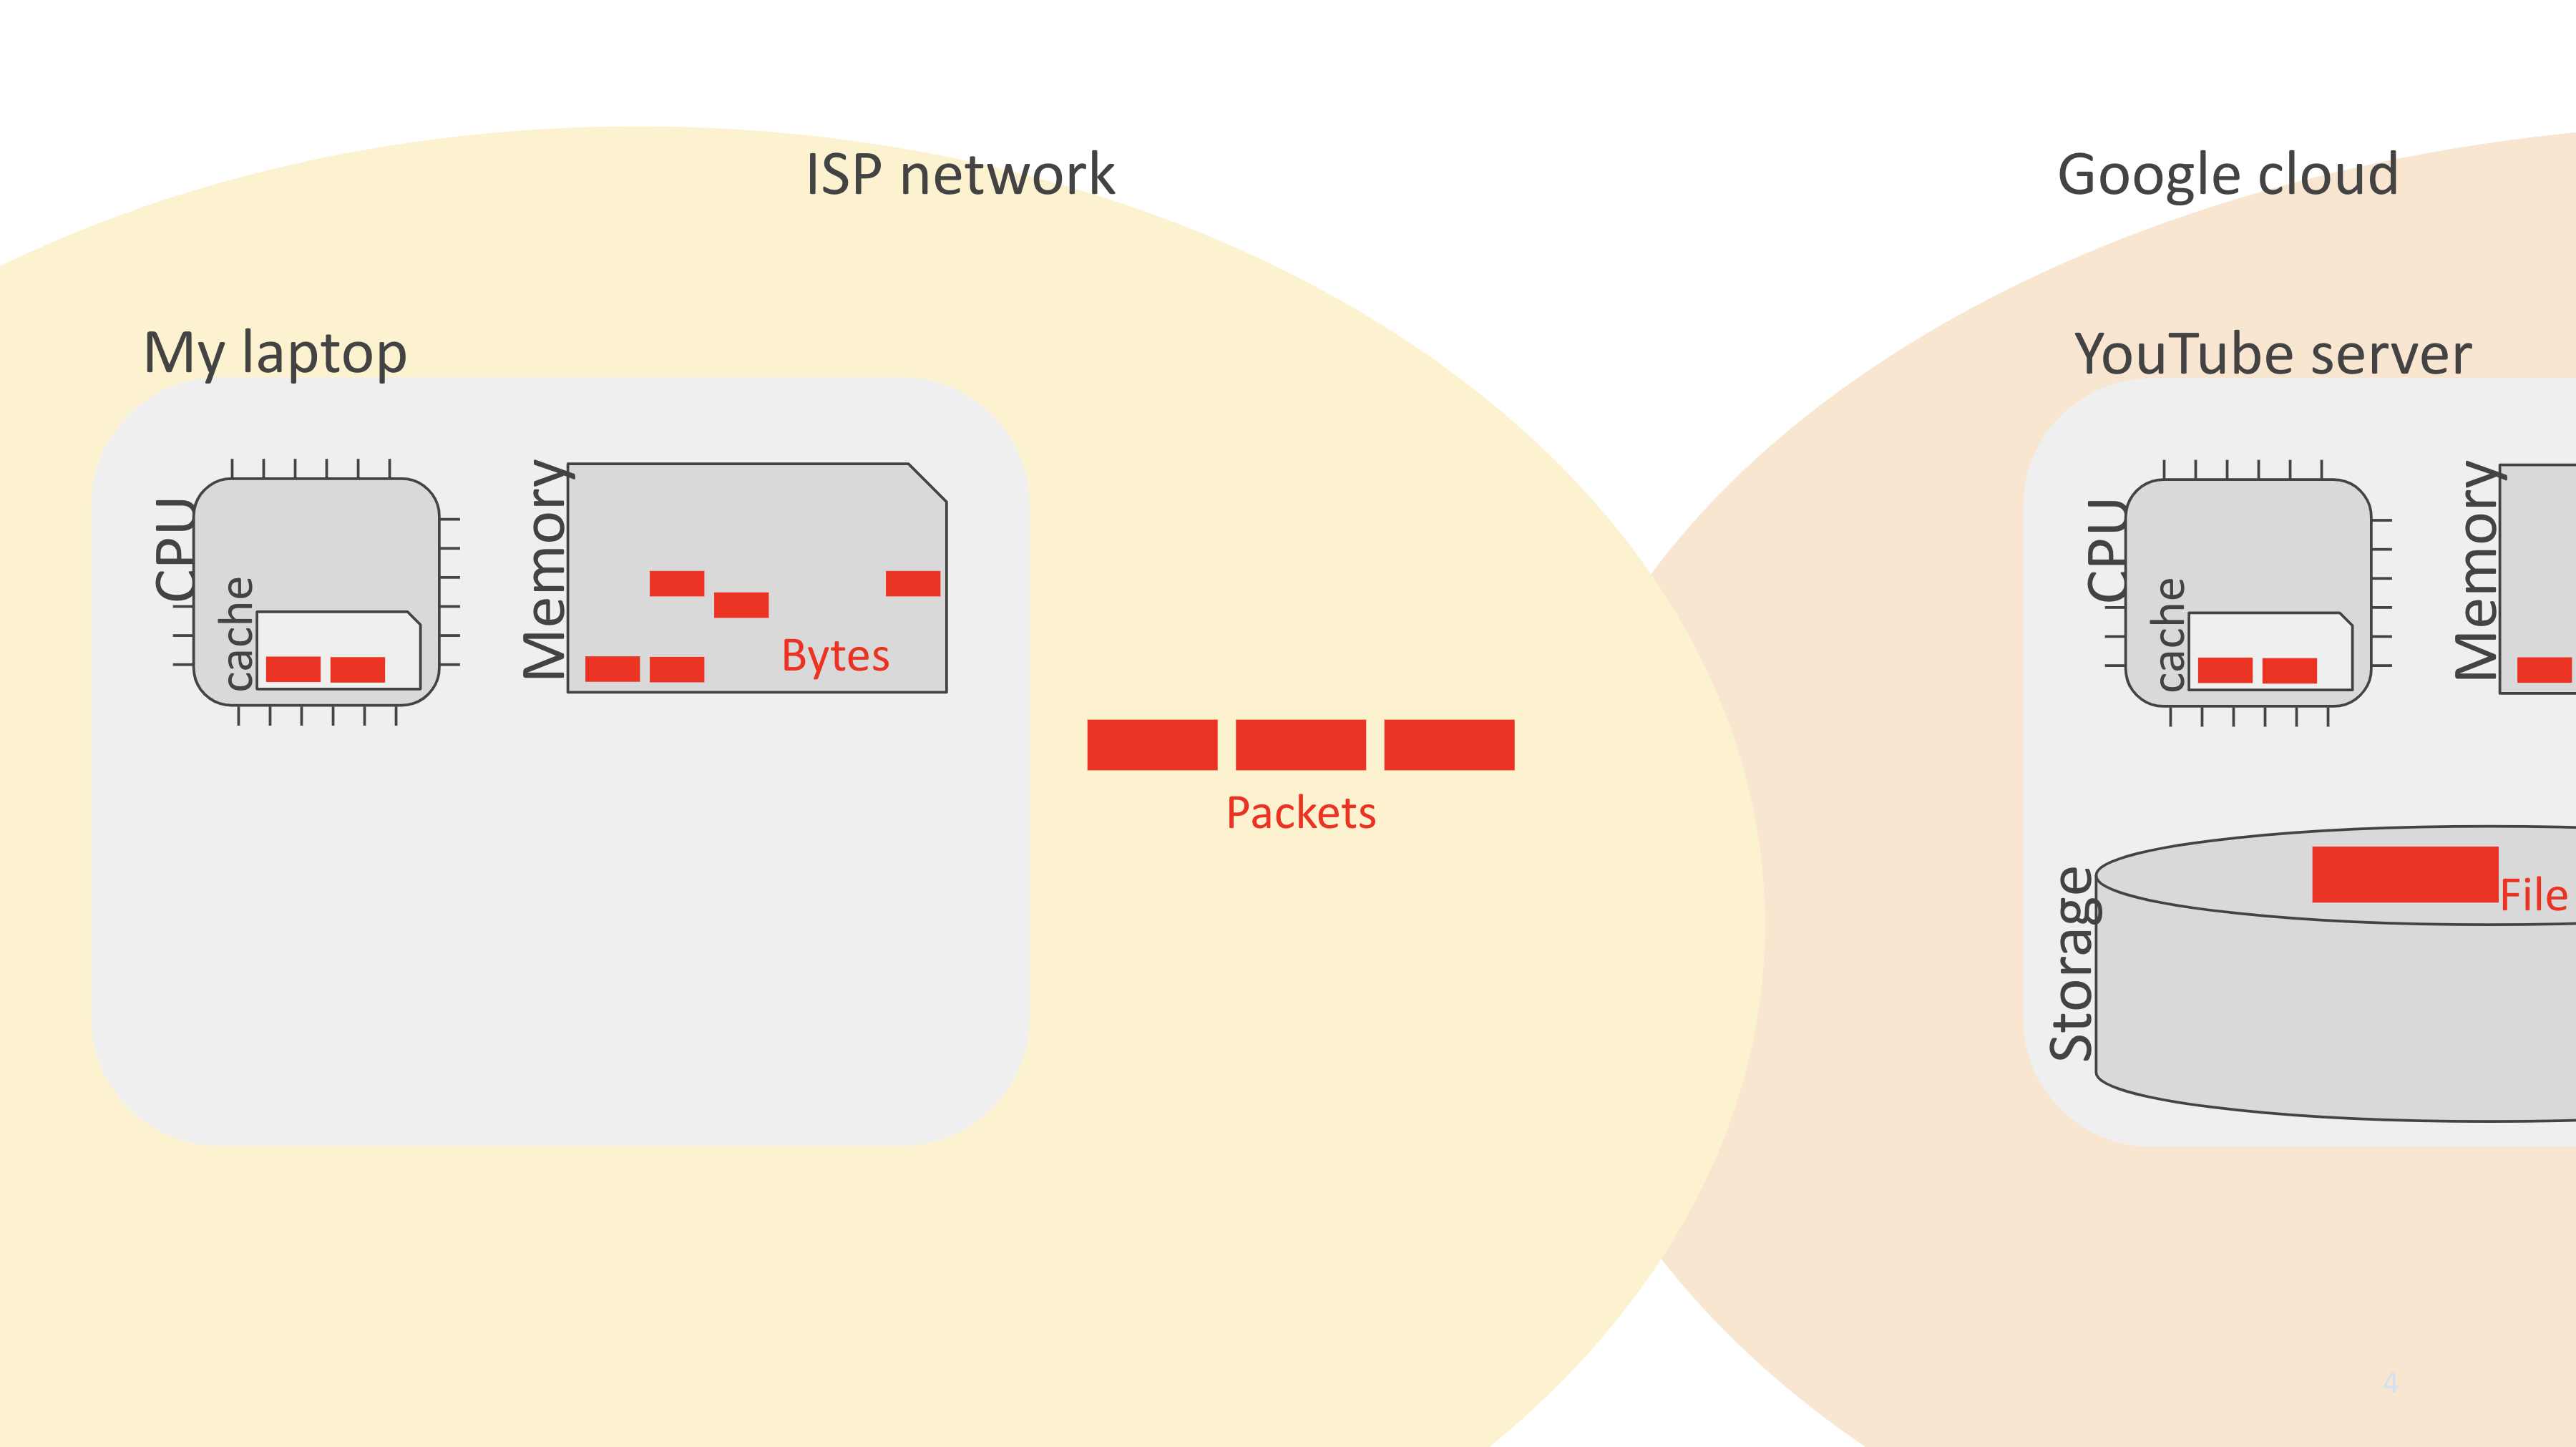
\includegraphics[width=0.85\textwidth]{chapters/L1/images/youtube.png}
\end{center}
\newpage
%%%%%%%%%%%%%%%%%%%%%%%%%%%%%%%%%%%%%%%%%%%%%%%%%%%%%%%%%%%%%%%%%%%%%%
\subsection{Start of the Journey: Inside the Laptop}
The journey begins on your laptop.\\[5px] 
\begin{minipage}{0.45\textwidth}
  \begin{justify}
    A computer hosts many different programs (e.g., a web browser, a ping utility, a git client). These programs, stored as files on disk, are invoked by user actions such as clicking an icon or typing a command. When a program is invoked, the computer creates a new \emph{process} in main memory. A process represents a running instance of a program and may consist of one or more \emph{threads}—individual units of execution within the process.
  \end{justify}
\end{minipage}
\hfill
\vline
\hfill
\begin{minipage}{0.45\textwidth}
  \begin{center}
  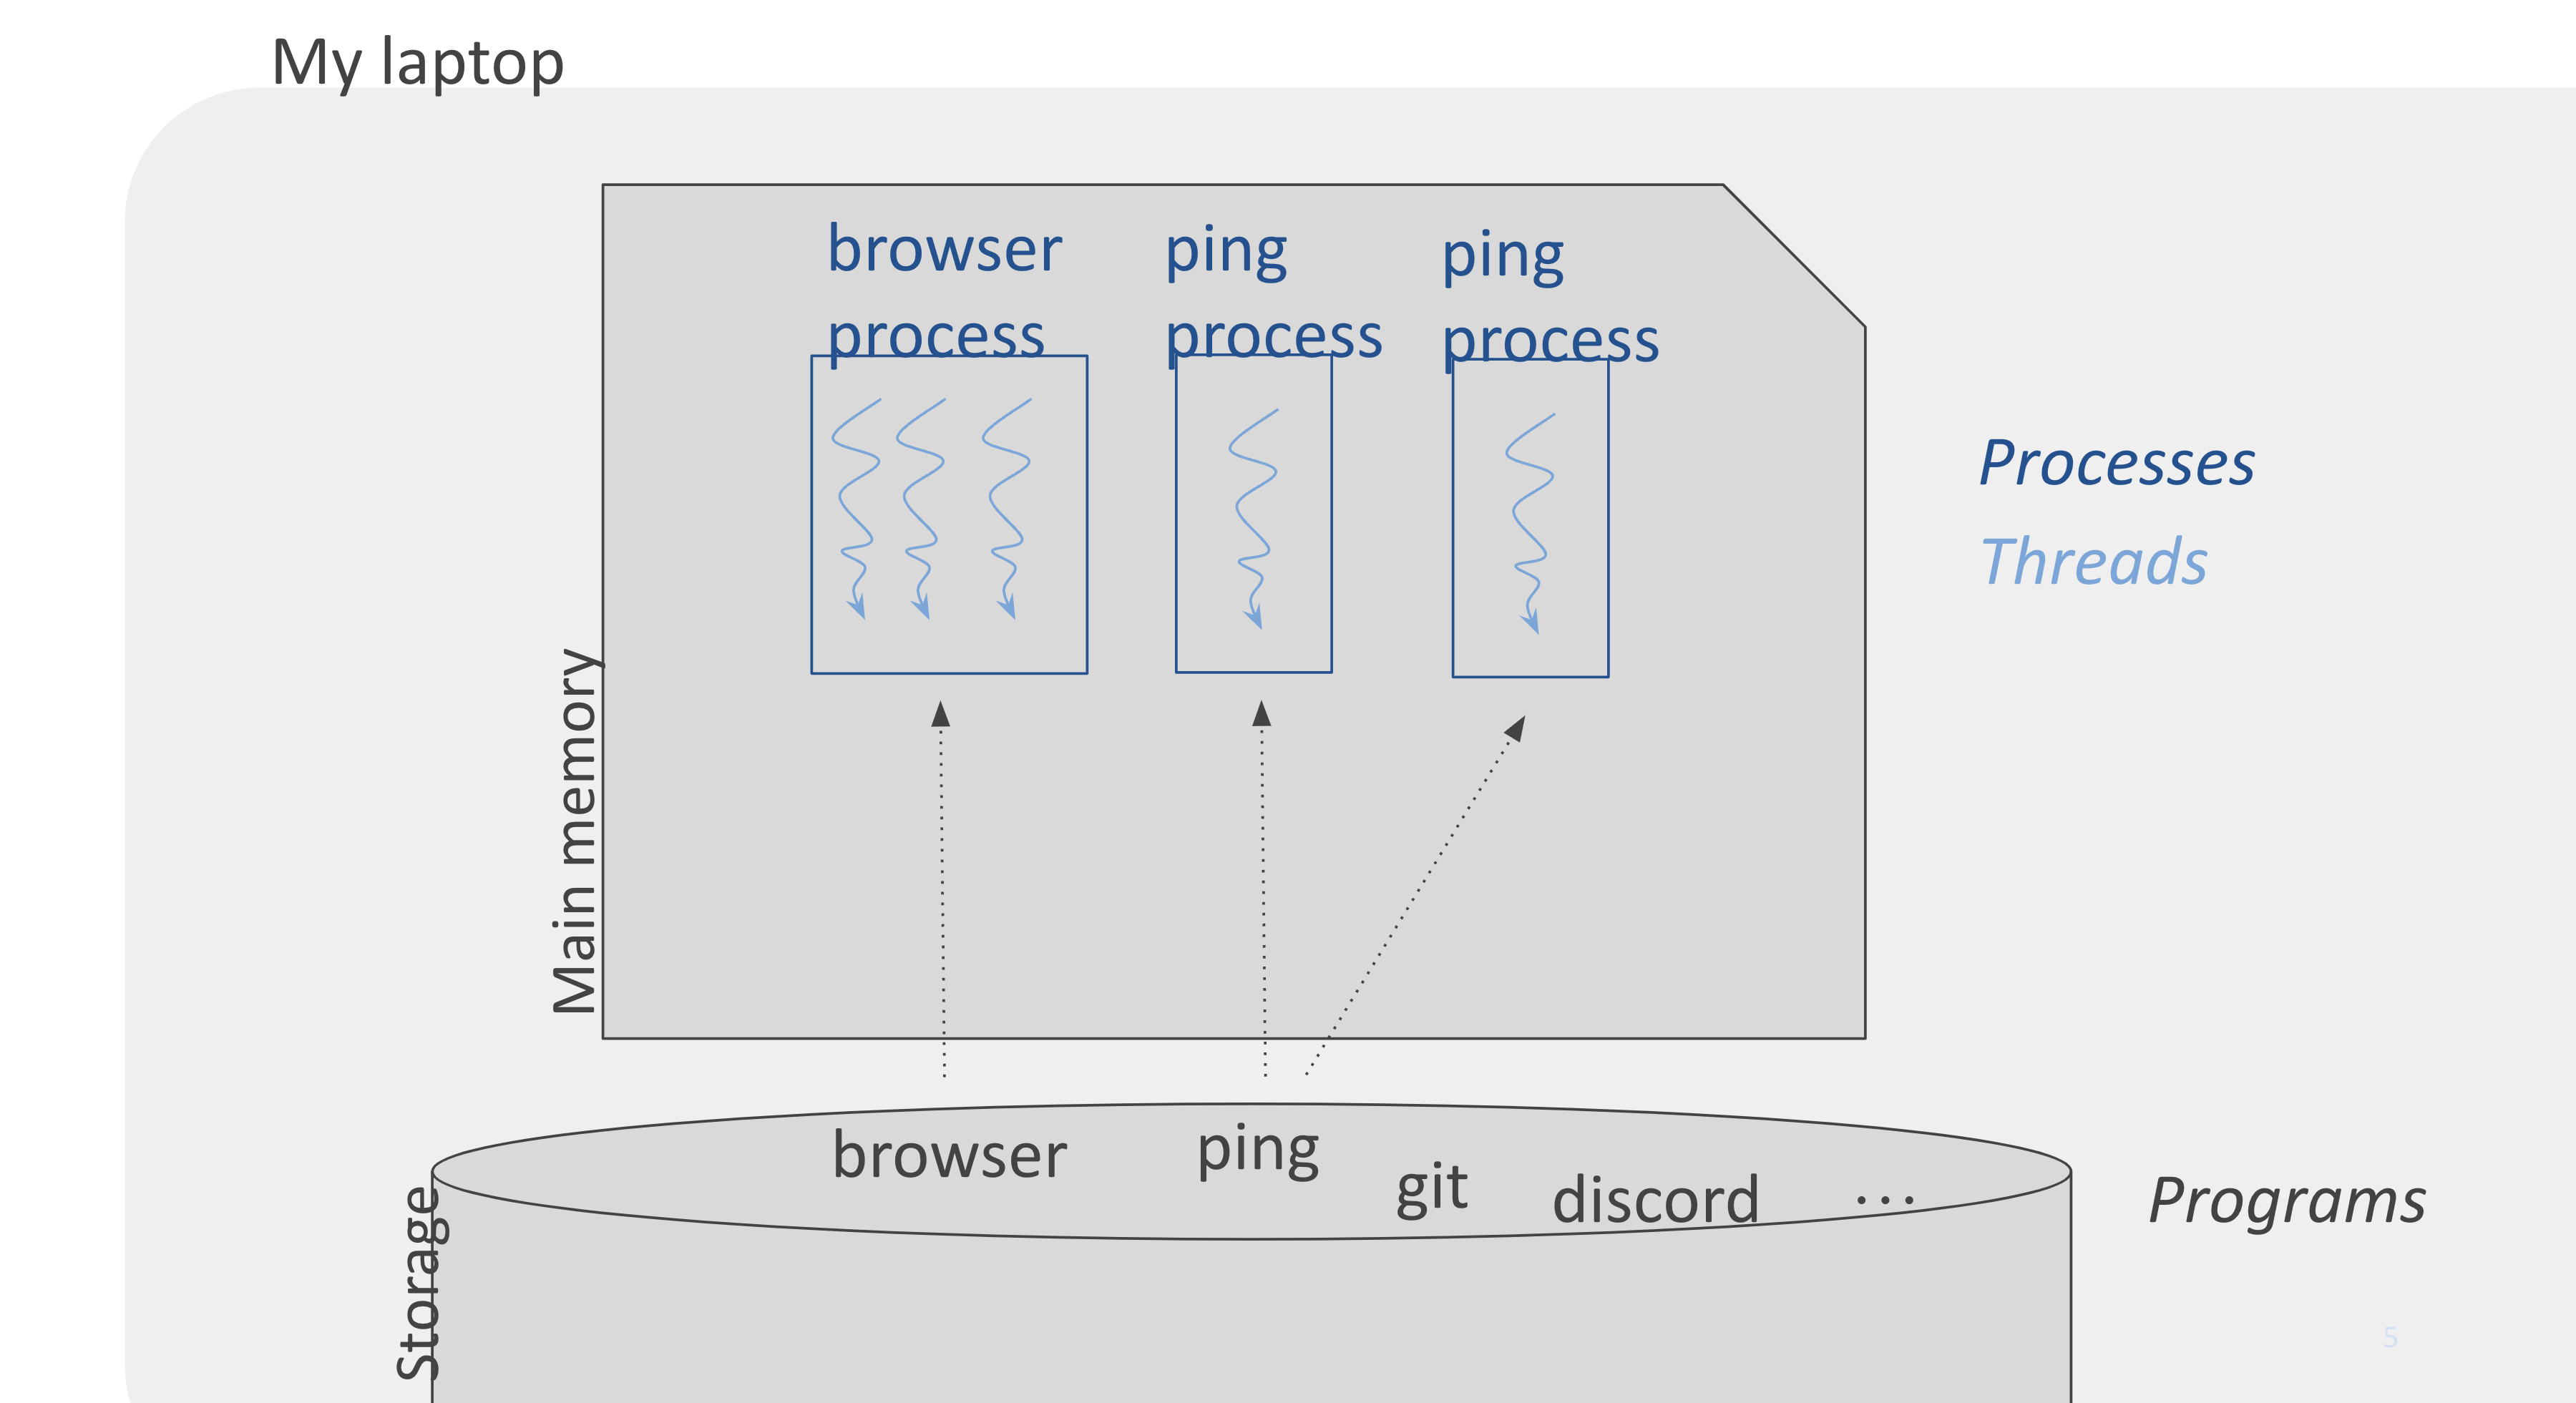
\includegraphics[width=1.2\textwidth]{chapters/L1/images/threads.png}
\end{center}
\end{minipage}\vfill
\vfill
\begin{definition}[Program, Process, Thread]
A \textbf{program} is a set of instructions stored as a file on disk. When a program is invoked, the computer creates a \textbf{process}—a running instance of that program in main memory. A process may consist of one or more \textbf{threads}, which are the individual sequences of execution within the process.
\end{definition}

%%%%%%%%%%%%%%%%%%%%%%%%%%%%%%%%%%%%%%%%%%%%%%%%%%%%%%%%%%%%%%%%%%%%%jjjj%
\vfill
\subsection{Accessing a Video: A Distributed Application}

When you use your web browser to access a video, the browser sends a message (or request) to a remote YouTube server. The browser process (running on your laptop) and the server process (running on a different computer) work together as parts of a \emph{distributed application}. 
\begin{center}
  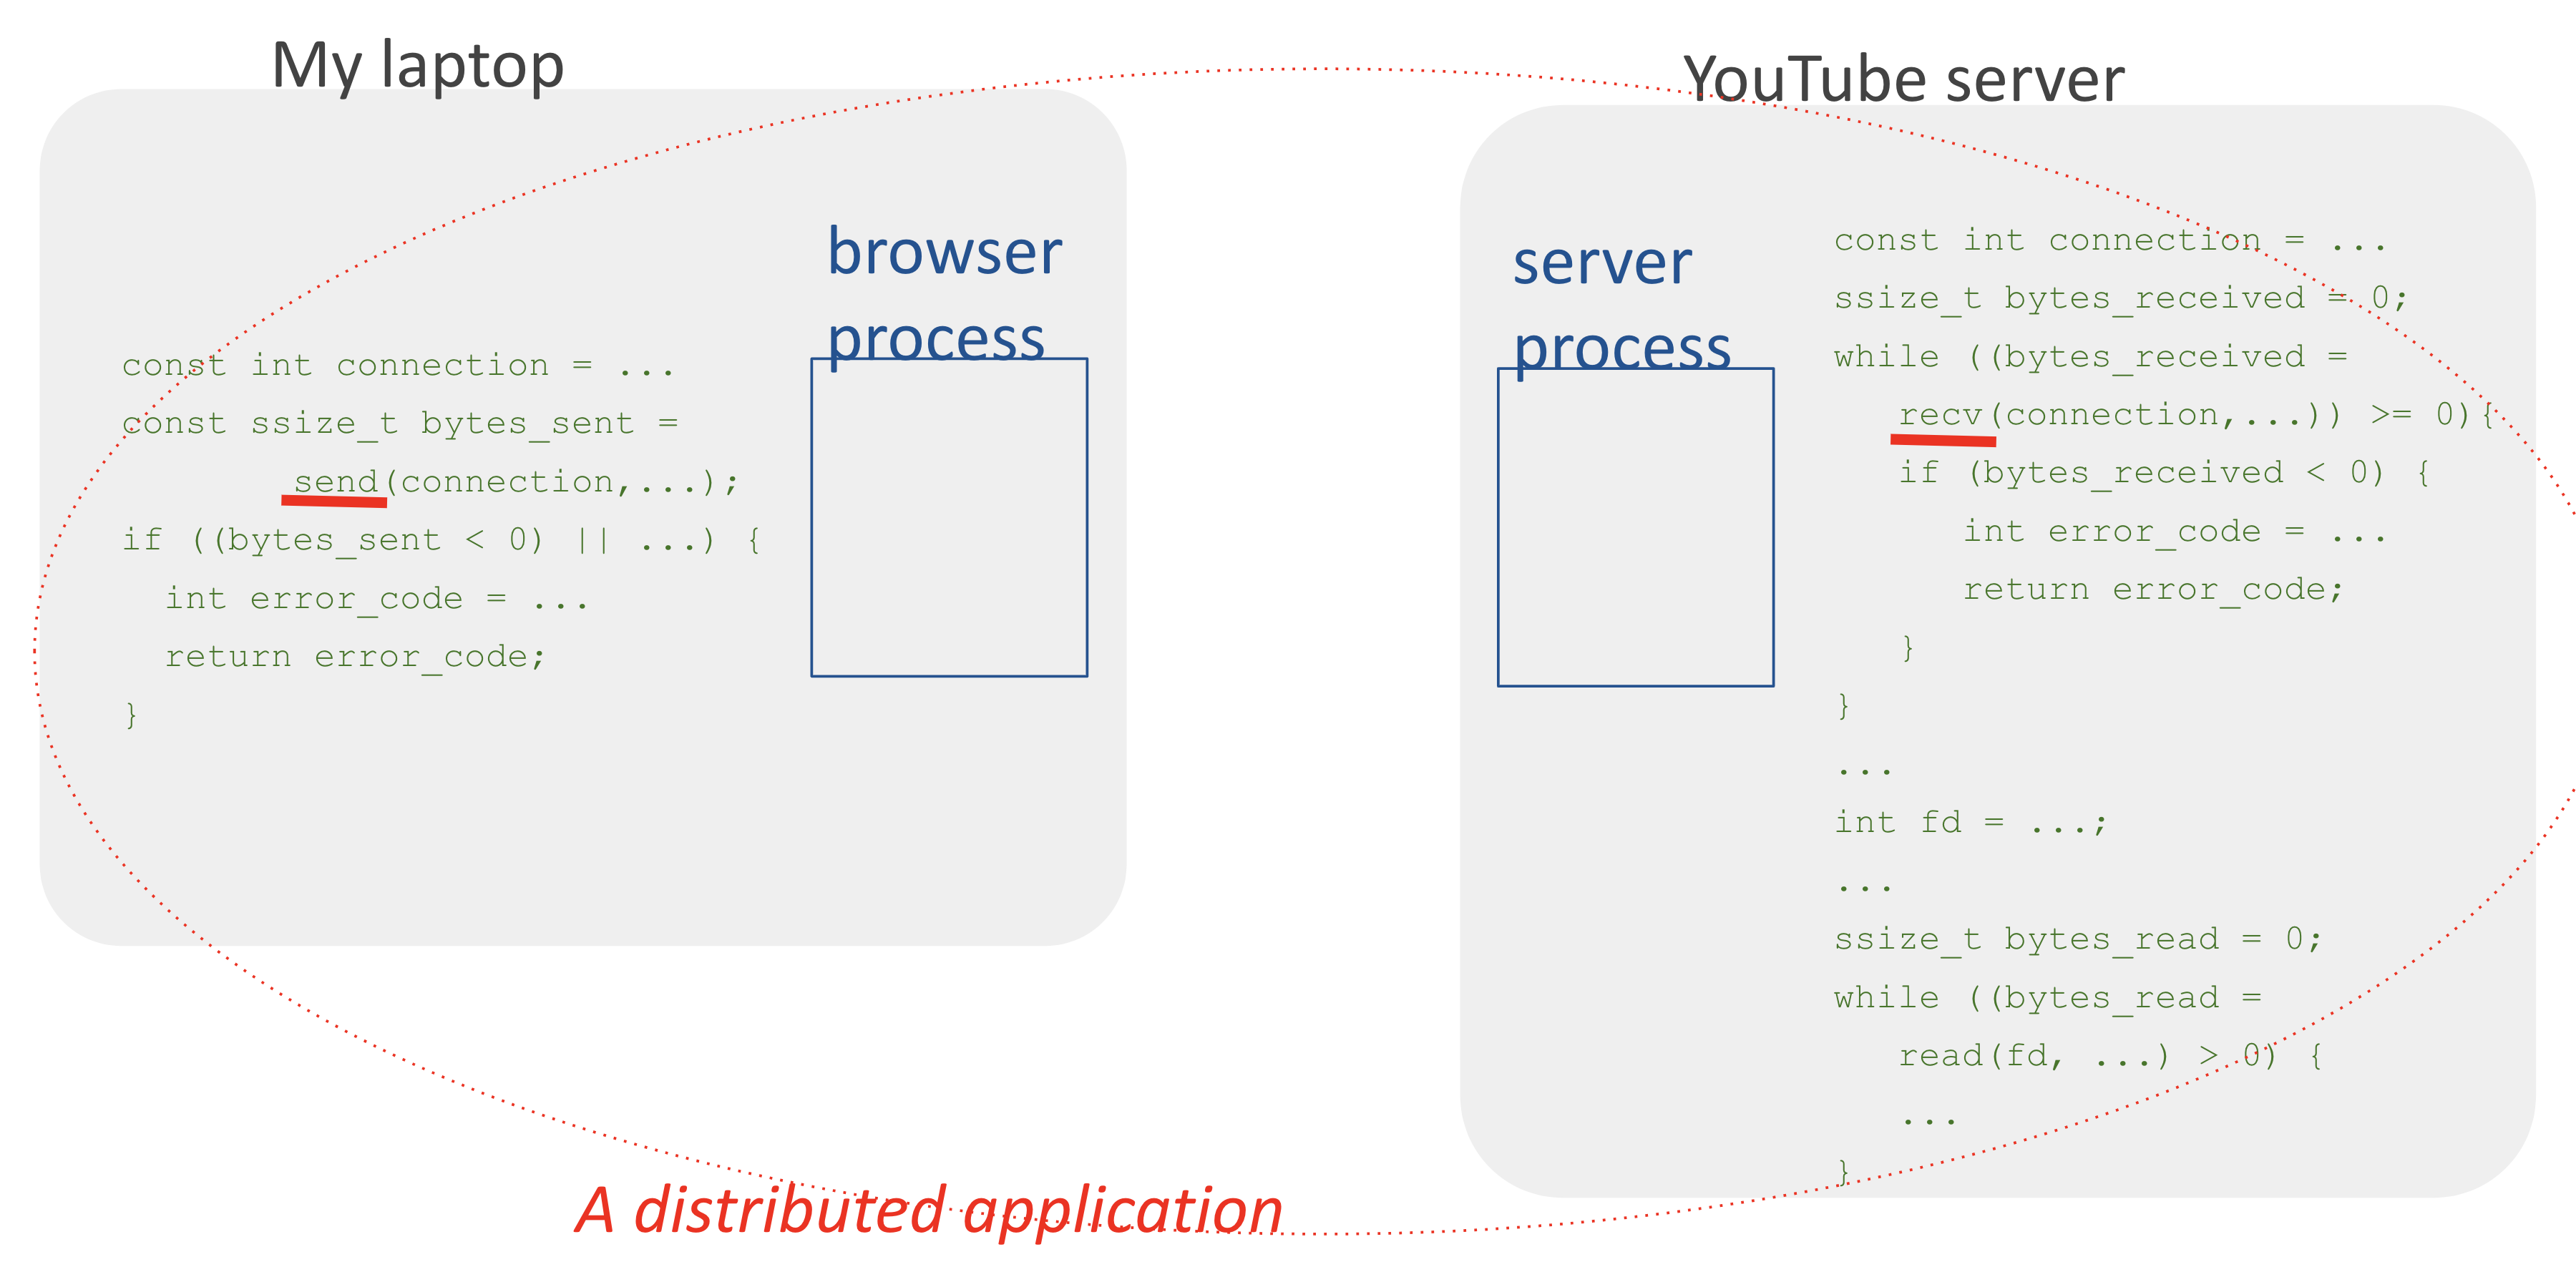
\includegraphics[width=0.95\textwidth]{chapters/L1/images/distributed.png}
\end{center}

%%%%%%%%%%%%%%%%%%%%%%%%%%%%%%%%%%%%%%%%%%%%%%%%%%%%%%%%%%%%%%%%%%%%%%
\newpage
\subsection{Communication Protocols}
For two processes running on different devices to work together, they must follow a predetermined set of rules known as a \textbf{communication protocol}. For example, a simple protocol might involve:
\begin{itemize}
  \item[-] One process sending “hello” and waiting for a “hello back.”
  \item[-] A subsequent request for a specific file (e.g., \texttt{xyz}) with the server responding with the file or an error message.
\end{itemize}
Much like human communication, these protocols ensure that both parties know what to expect, enabling effective interaction.

\begin{center}
  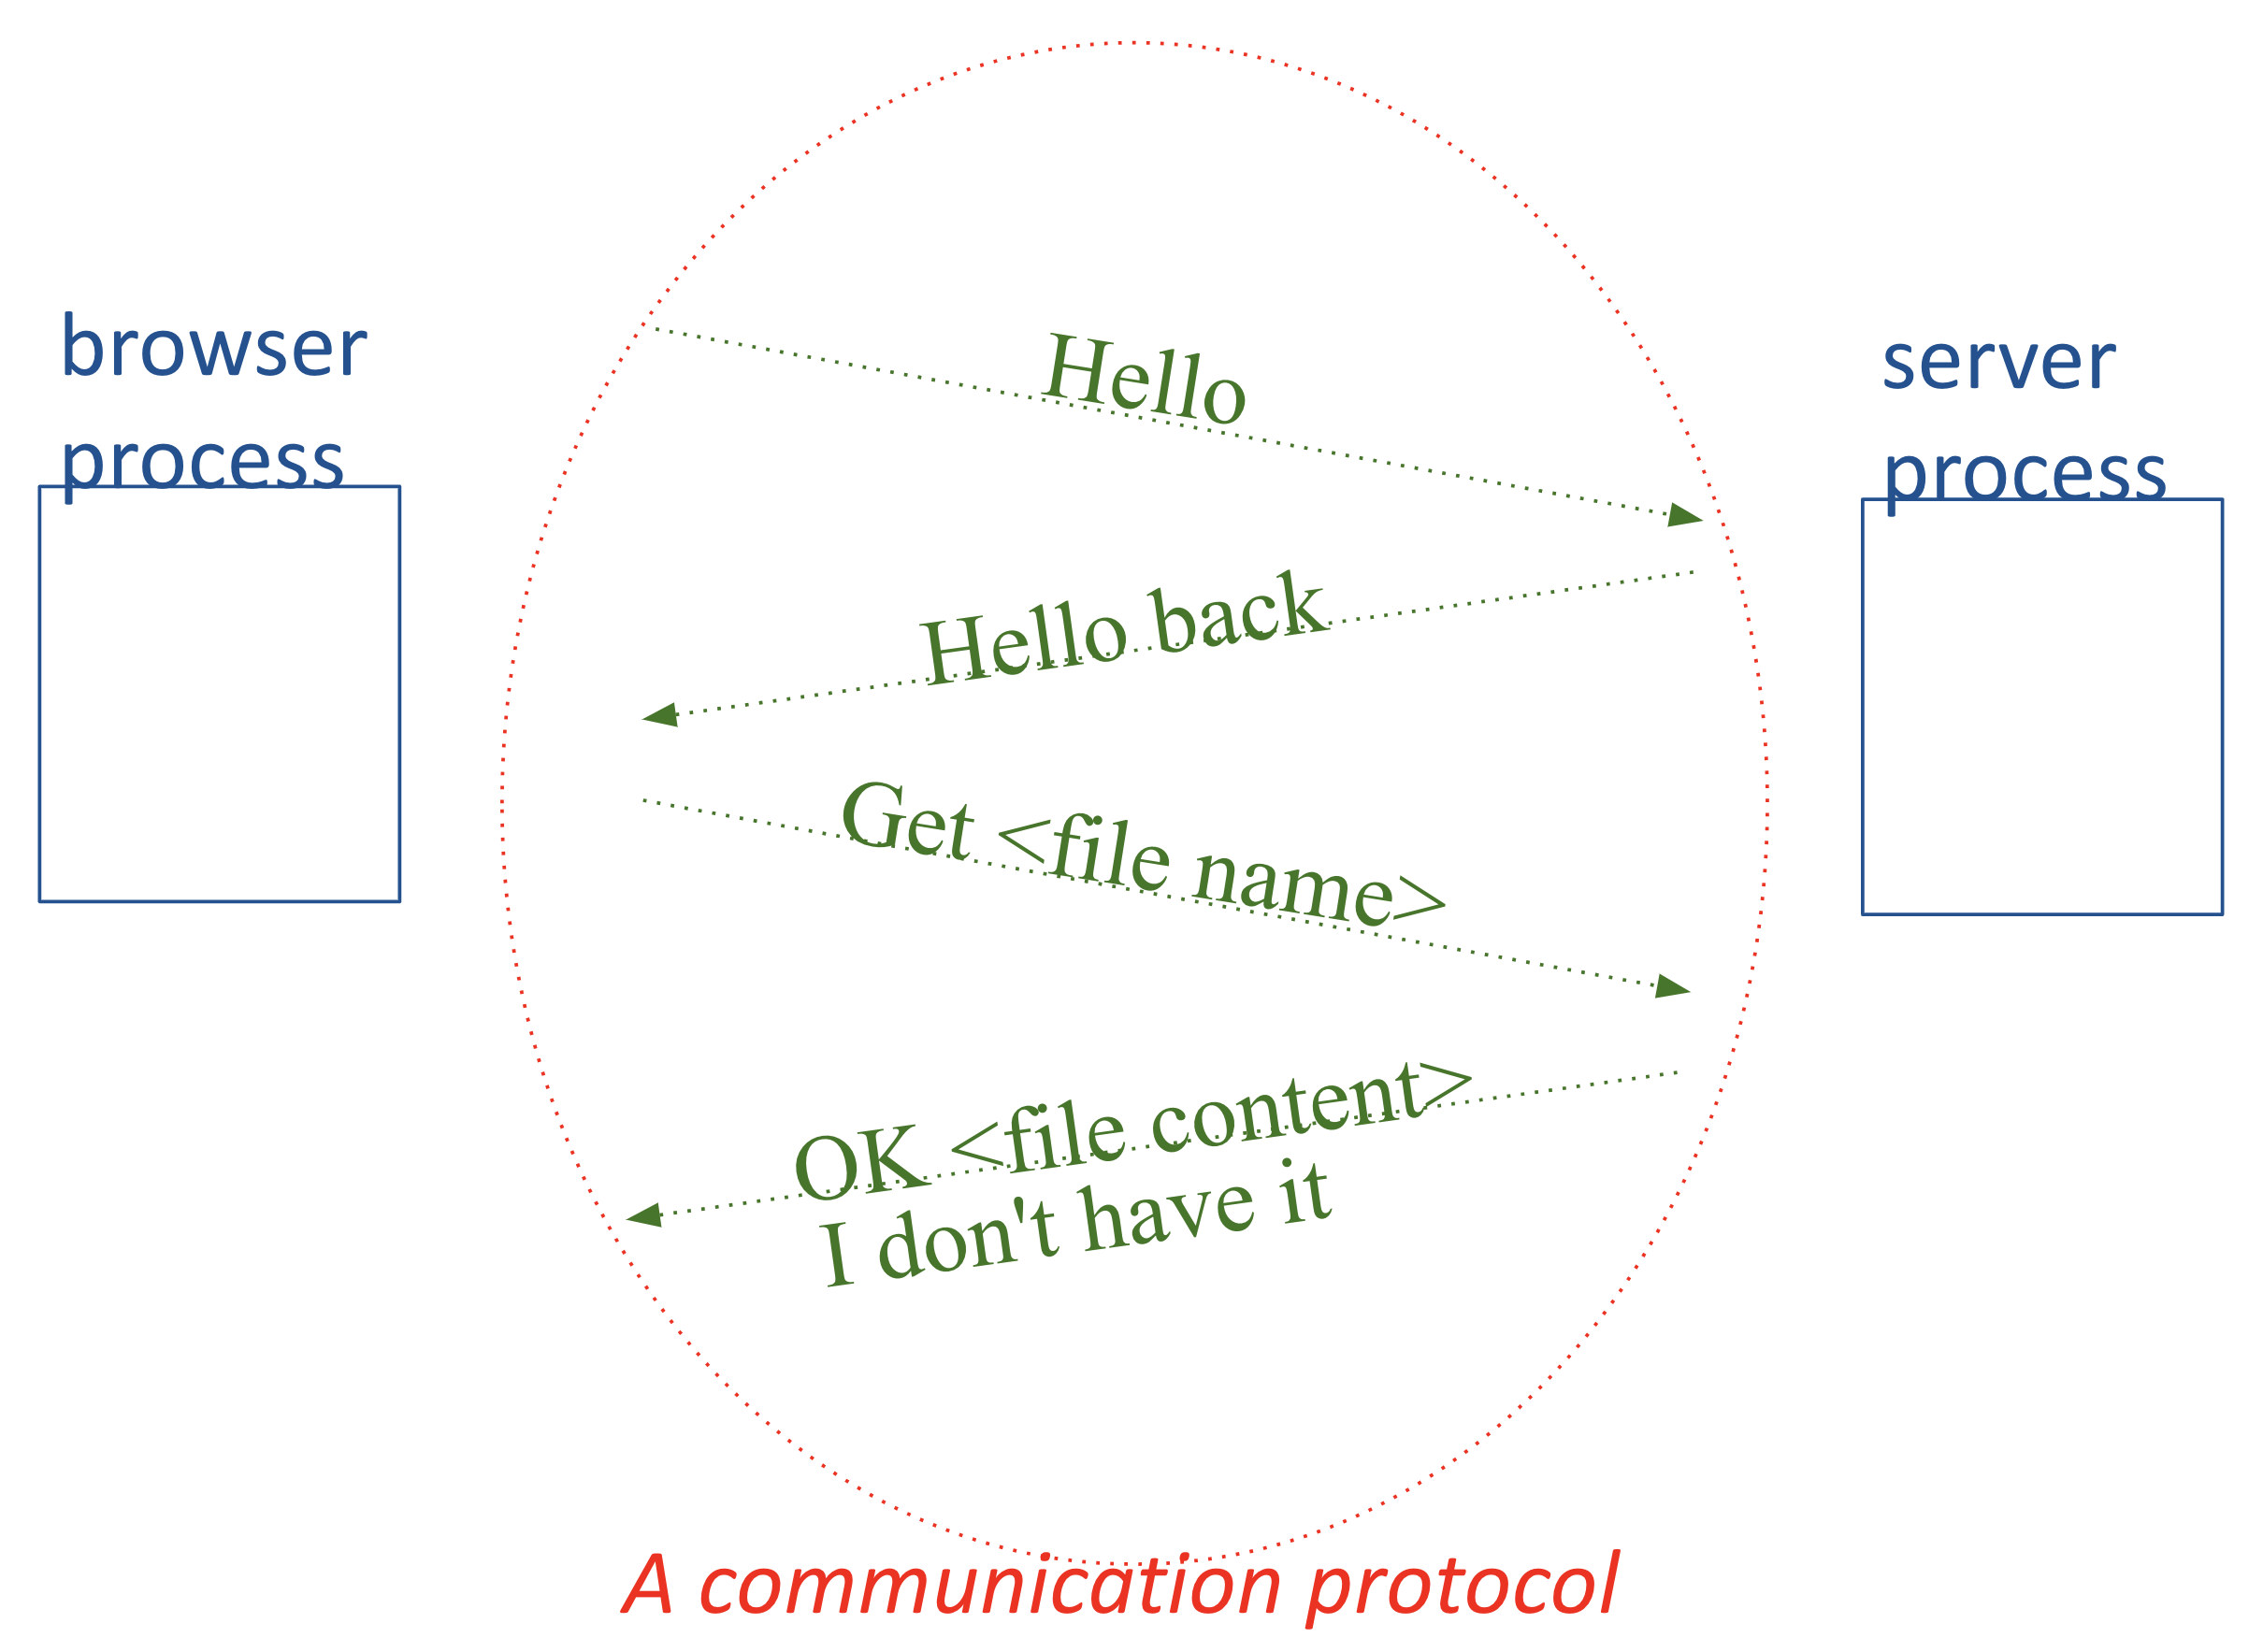
\includegraphics[width=0.45\textwidth]{chapters/L1/images/comm_prot.png}
\end{center}

%%%%%%%%%%%%%%%%%%%%%%%%%%%%%%%%%%%%%%%%%%%%%%%%%%%%%%%%%%%%%%%%%%%%%%
\subsection{Distributed Applications and APIs}

Distributed applications consist of separate pieces of code running as processes on different machines but working toward a common goal. These processes exchange messages over the Internet by following communication protocols.  
To simplify the development of these applications, developers use \emph{system calls} (or \textbf{syscalls}). Syscalls are special functions provided by the operating system that allow processes to access resources (e.g., network and storage) without needing to know the low-level details.

The set of syscalls available to an application forms its \textbf{Application Programming Interface} (API), abstracting away the complexities of resource management.

\begin{center}
  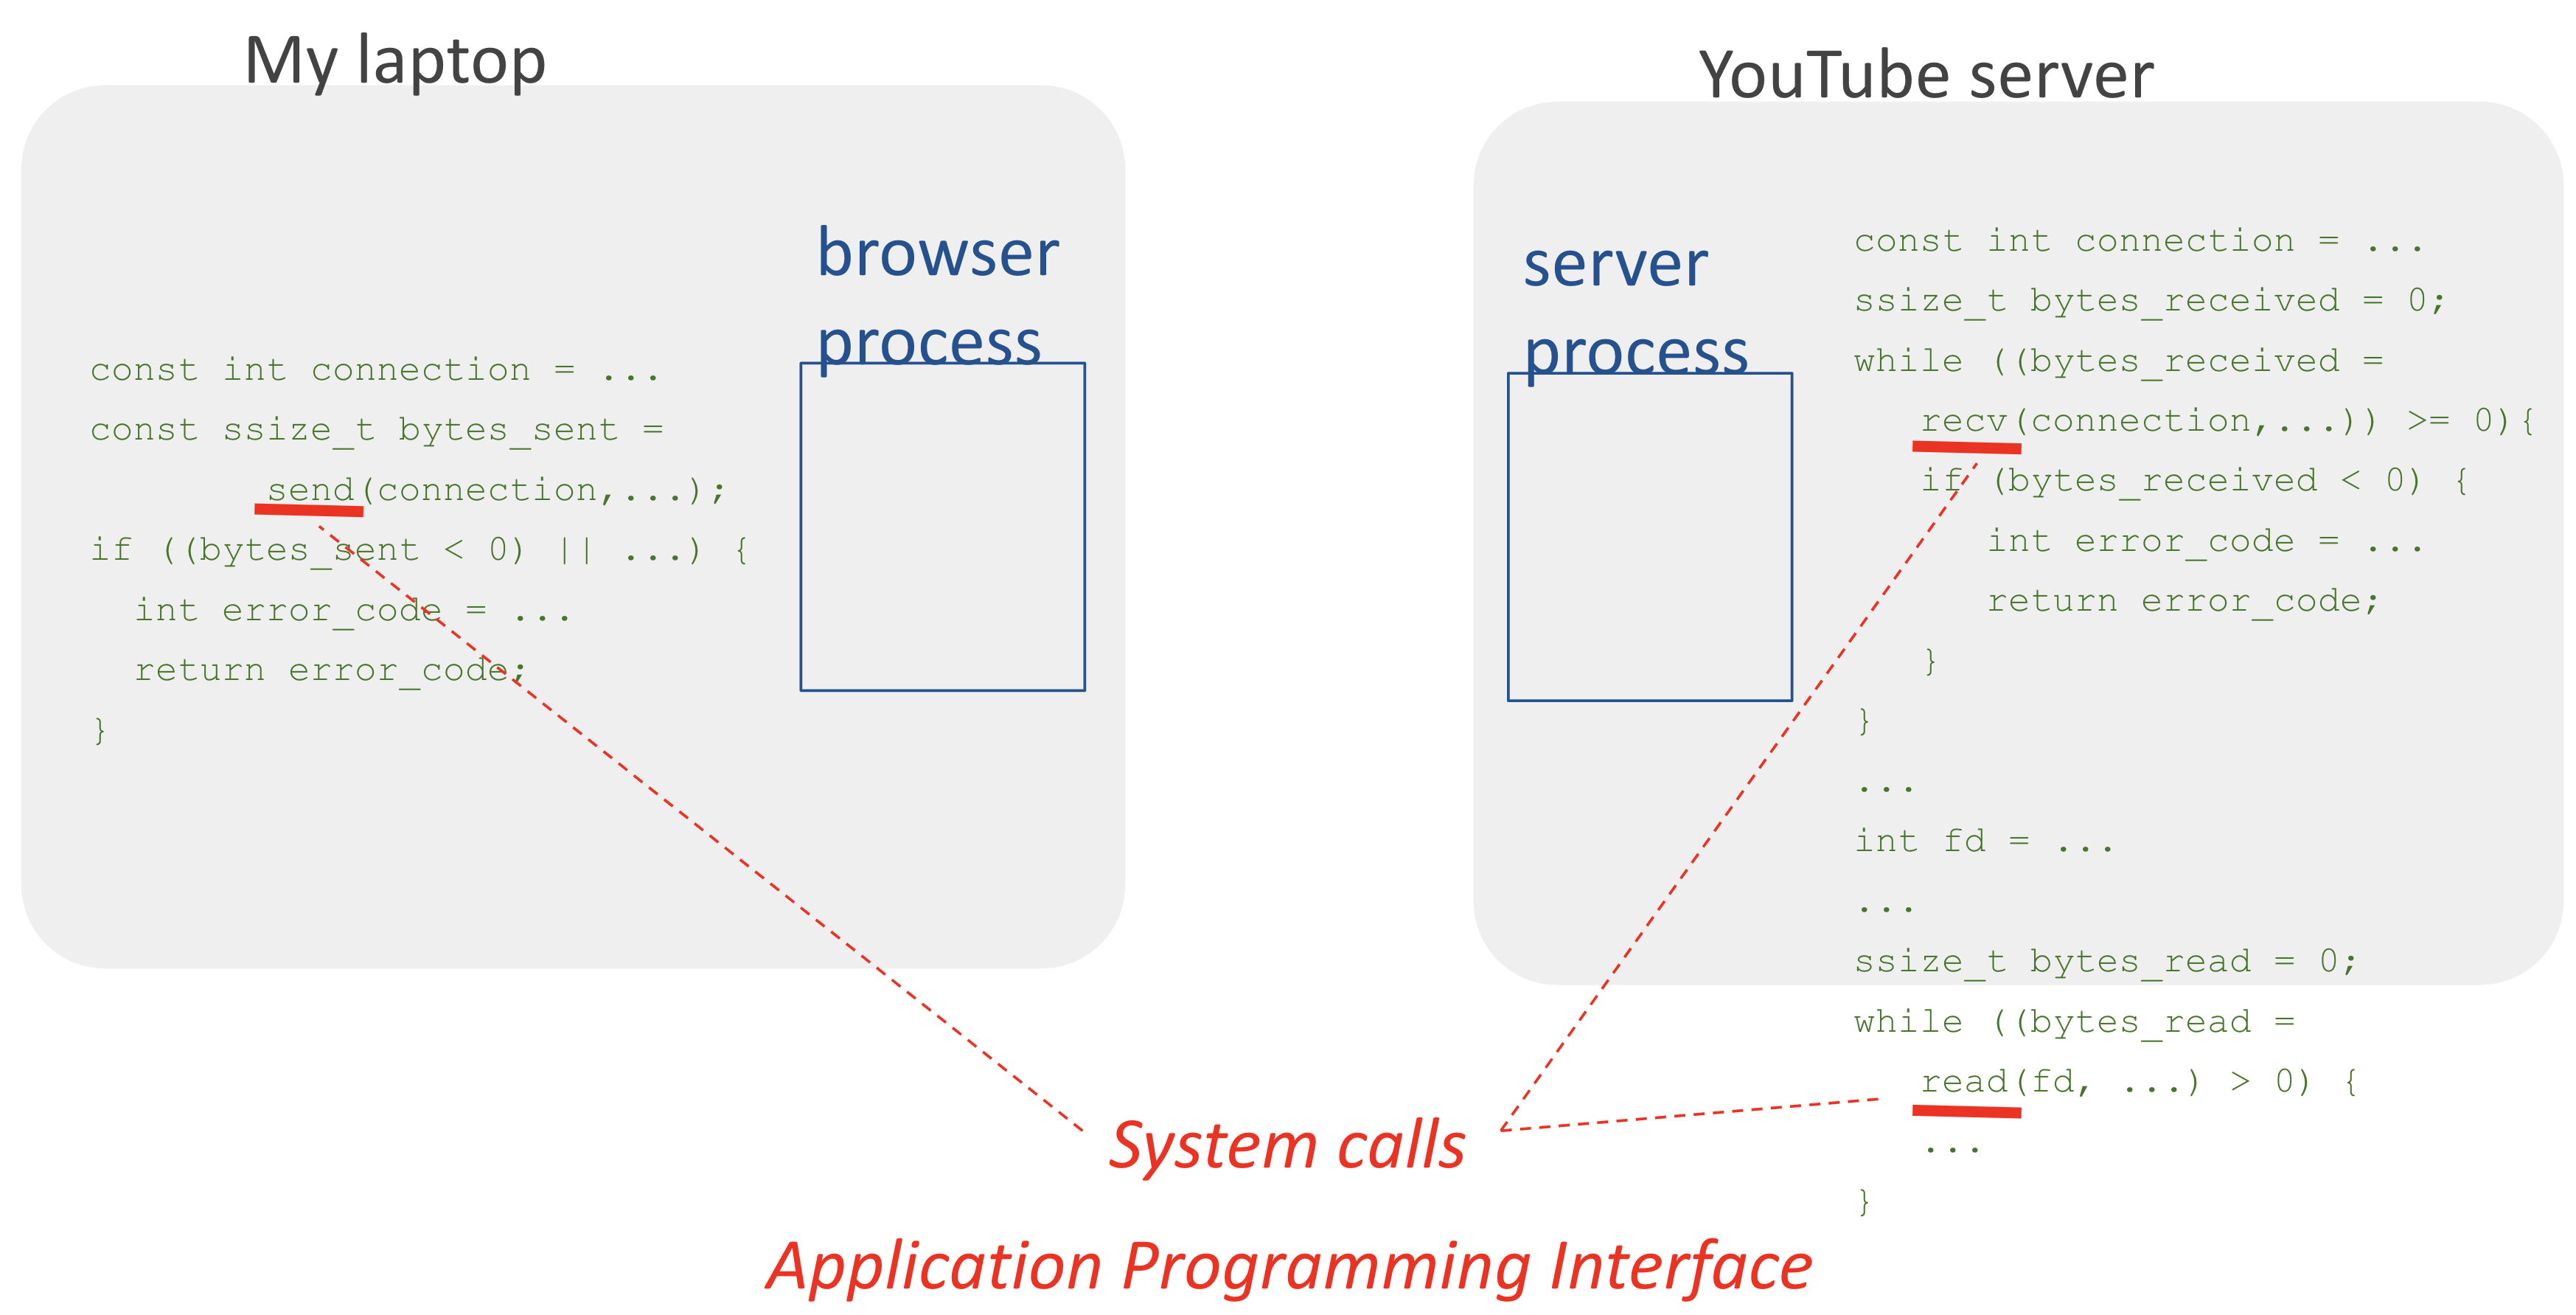
\includegraphics[width=0.85\textwidth]{chapters/L1/images/api.png}
\end{center}

%%%%%%%%%%%%%%%%%%%%%%%%%%%%%%%%%%%%%%%%%%%%%%%%%%%%%%%%%%%%%%%%%%%%%%
\vfill
\begin{definition}[Interface]
An \textbf{interface} is a set of rules that defines how different components communicate. For instance, when sending a letter via the postal system, one must follow specific rules (e.g., write the address and affix a stamp). This interface abstracts the complexities of the postal system so that users do not need to understand its internal operations.
\end{definition}

\begin{center}
  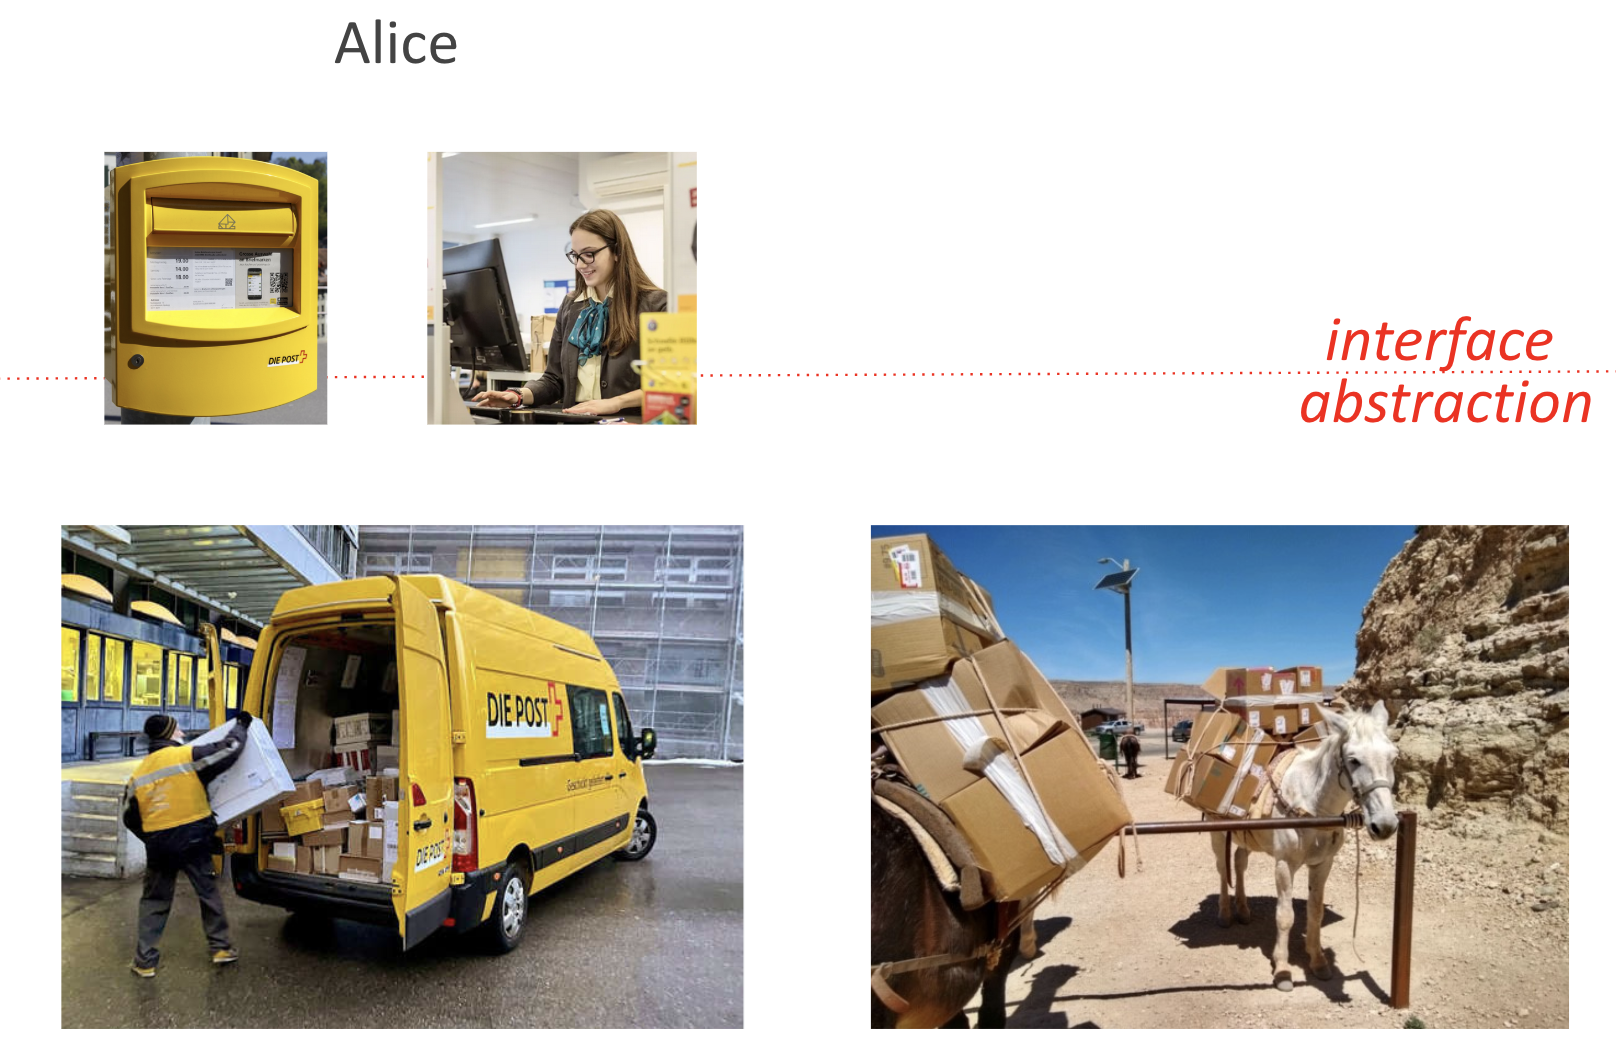
\includegraphics[width=0.65\textwidth]{chapters/L1/images/postal.png}
\end{center}
\vfill
%%%%%%%%%%%%%%%%%%%%%%%%%%%%%%%%%%%%%%%%%%%%%%%%%%%%%%%%%%%%%%%%%%%%%%
\subsection{System Calls (Syscalls)}

Syscalls form the interface between a process and external resources (like network and storage). They provide an abstraction of these resources, allowing a process to use them without knowing their intricate details. For example, when a process makes a syscall such as \texttt{send} or \texttt{recv}, the operating system’s network stack handles the details of the communication.

\begin{center}
  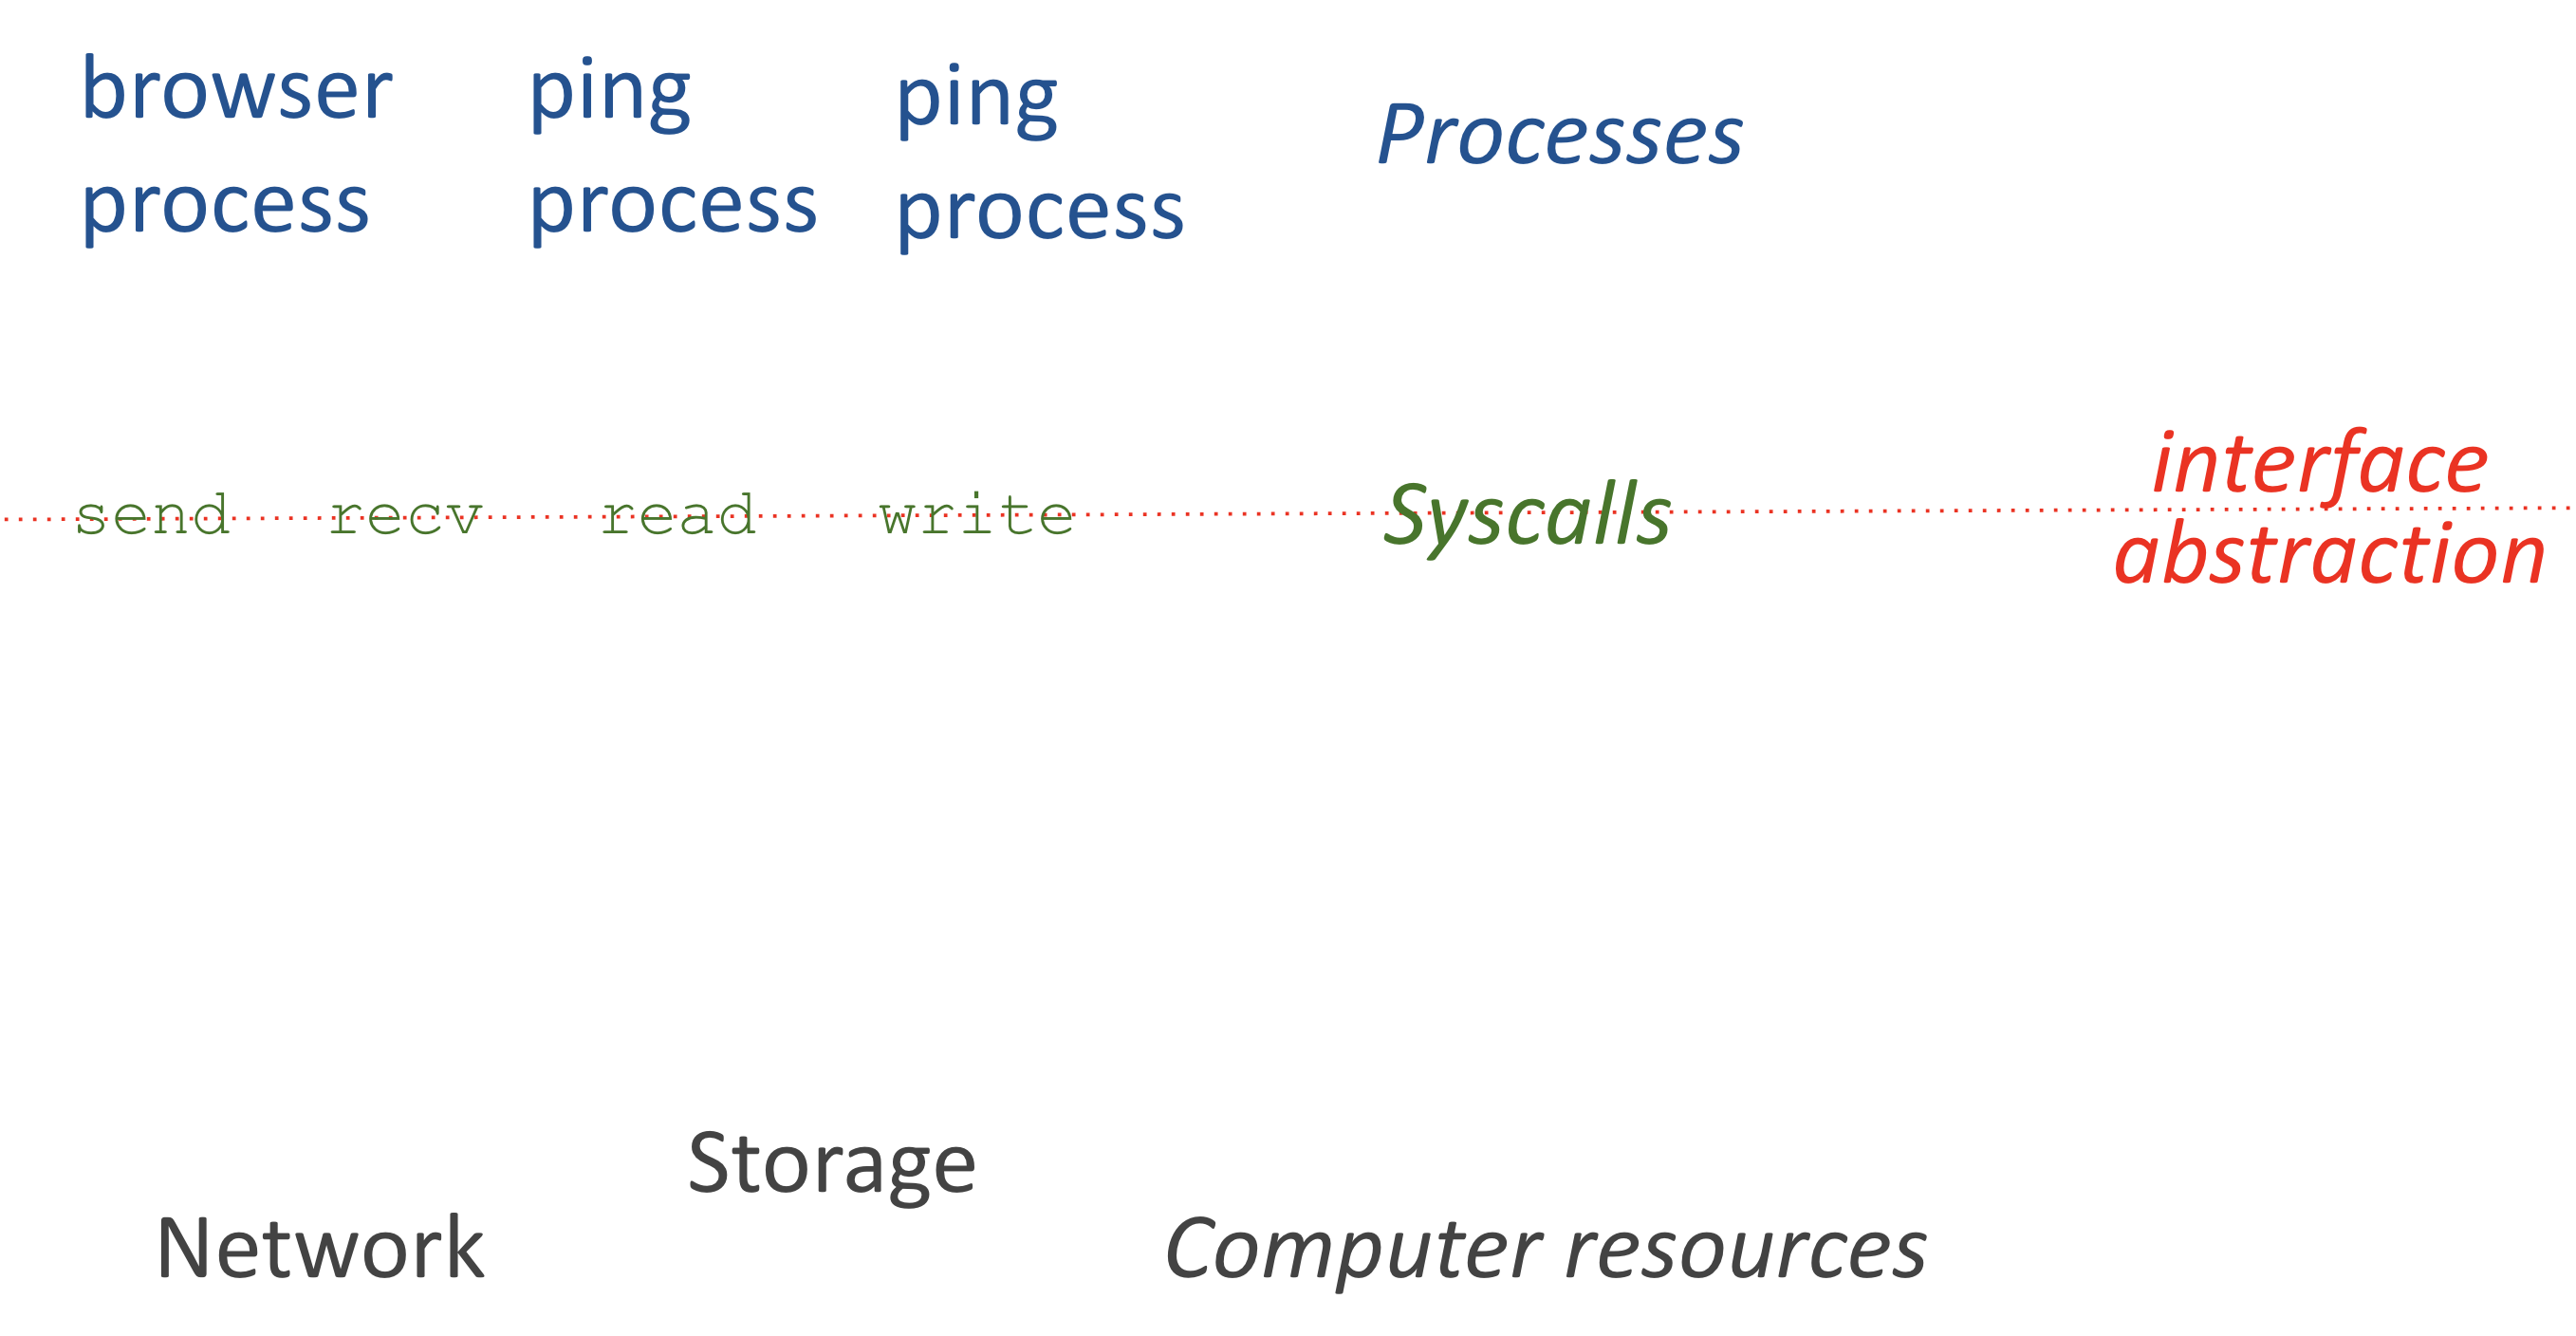
\includegraphics[width=0.65\textwidth]{chapters/L1/images/syscalls.png}
\end{center}
\vfill
\newpage
%%%%%%%%%%%%%%%%%%%%%%%%%%%%%%%%%%%%%%%%%%%%%%%%%%%%%%%%%%%%%%%%%%%%%%
\section{The Operating System}
Conceptually, the OS sits between running processes and the underlying hardware resources. It provides the syscall interface and handles tasks such as file system management and network communication. \\
\begin{minipage}{0.45\textwidth}
\begin{center}
  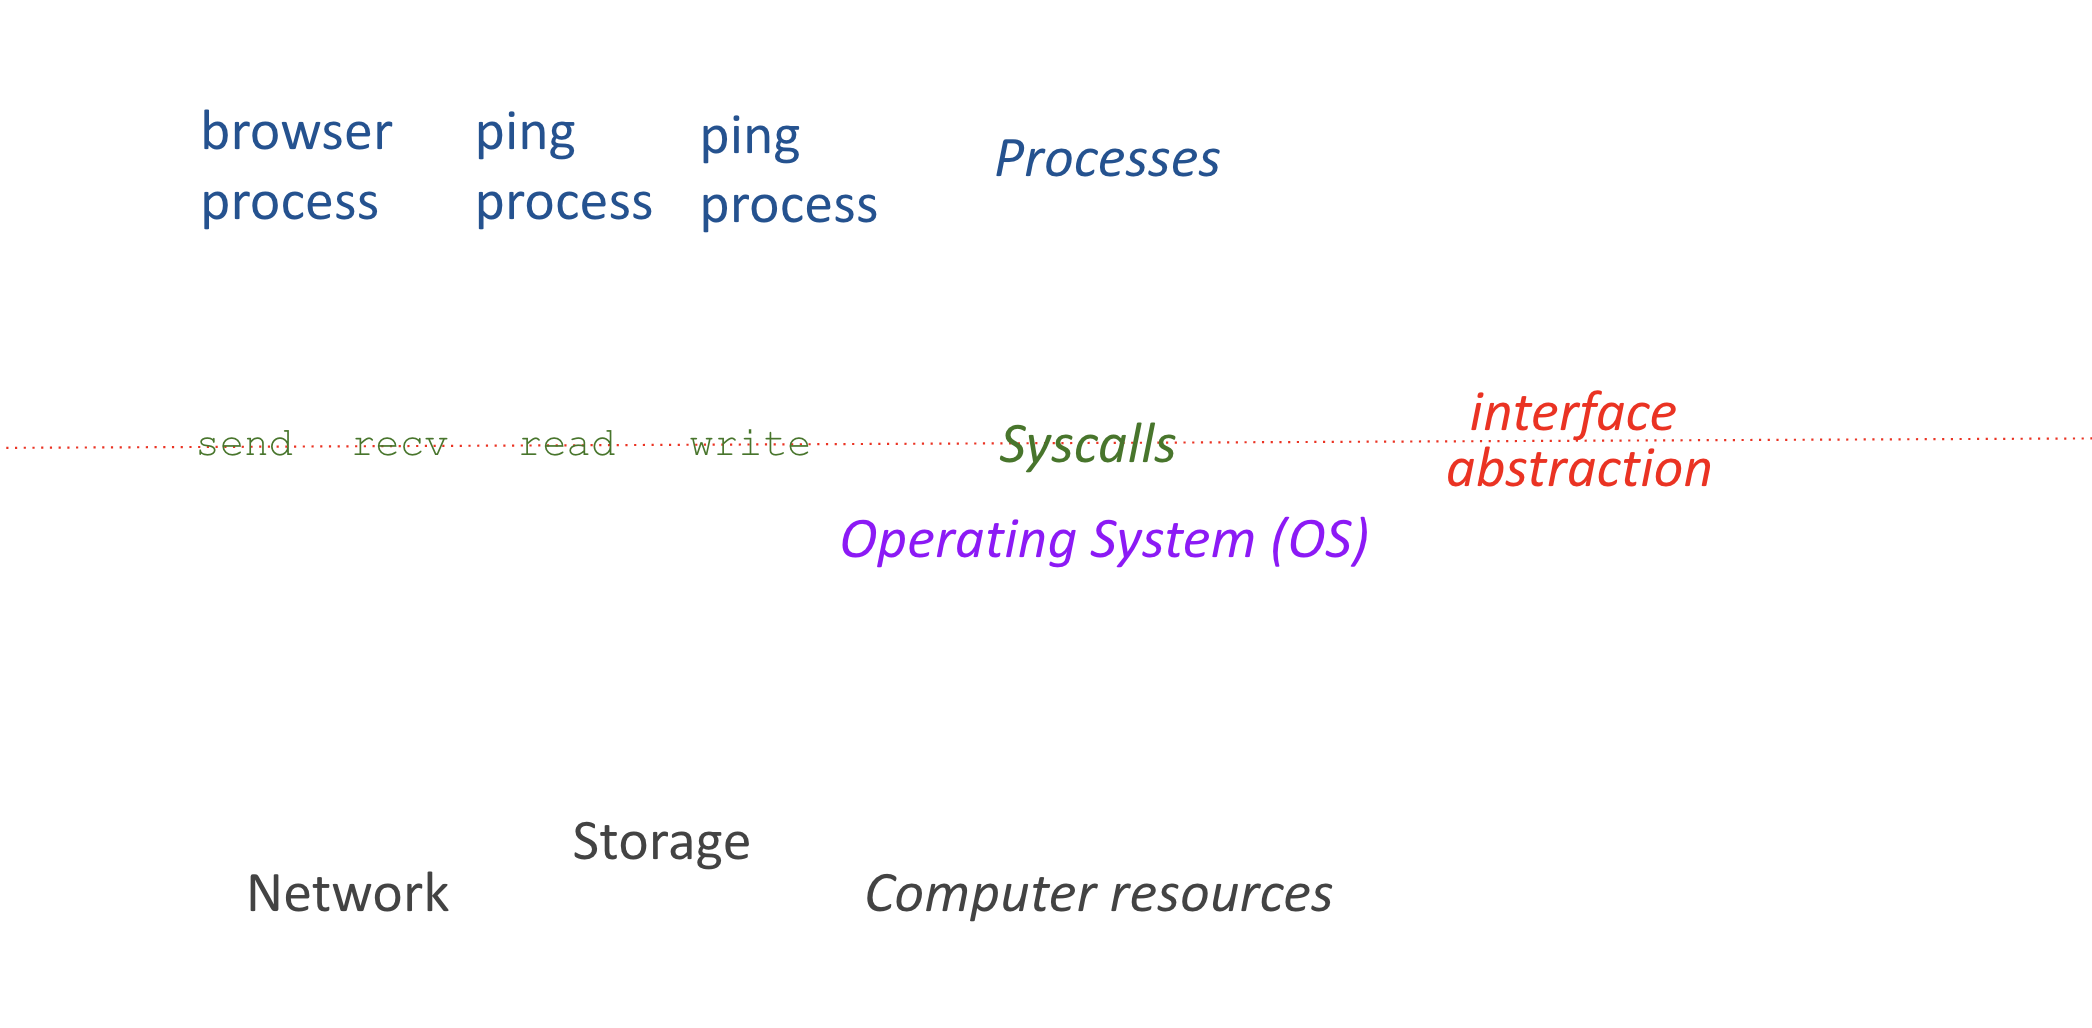
\includegraphics[width=1.15\textwidth]{chapters/L1/images/isa_os.png}
\end{center}
\end{minipage}
\hfill
\vline
\hfill
\begin{minipage}{0.45\textwidth}
\begin{center}
  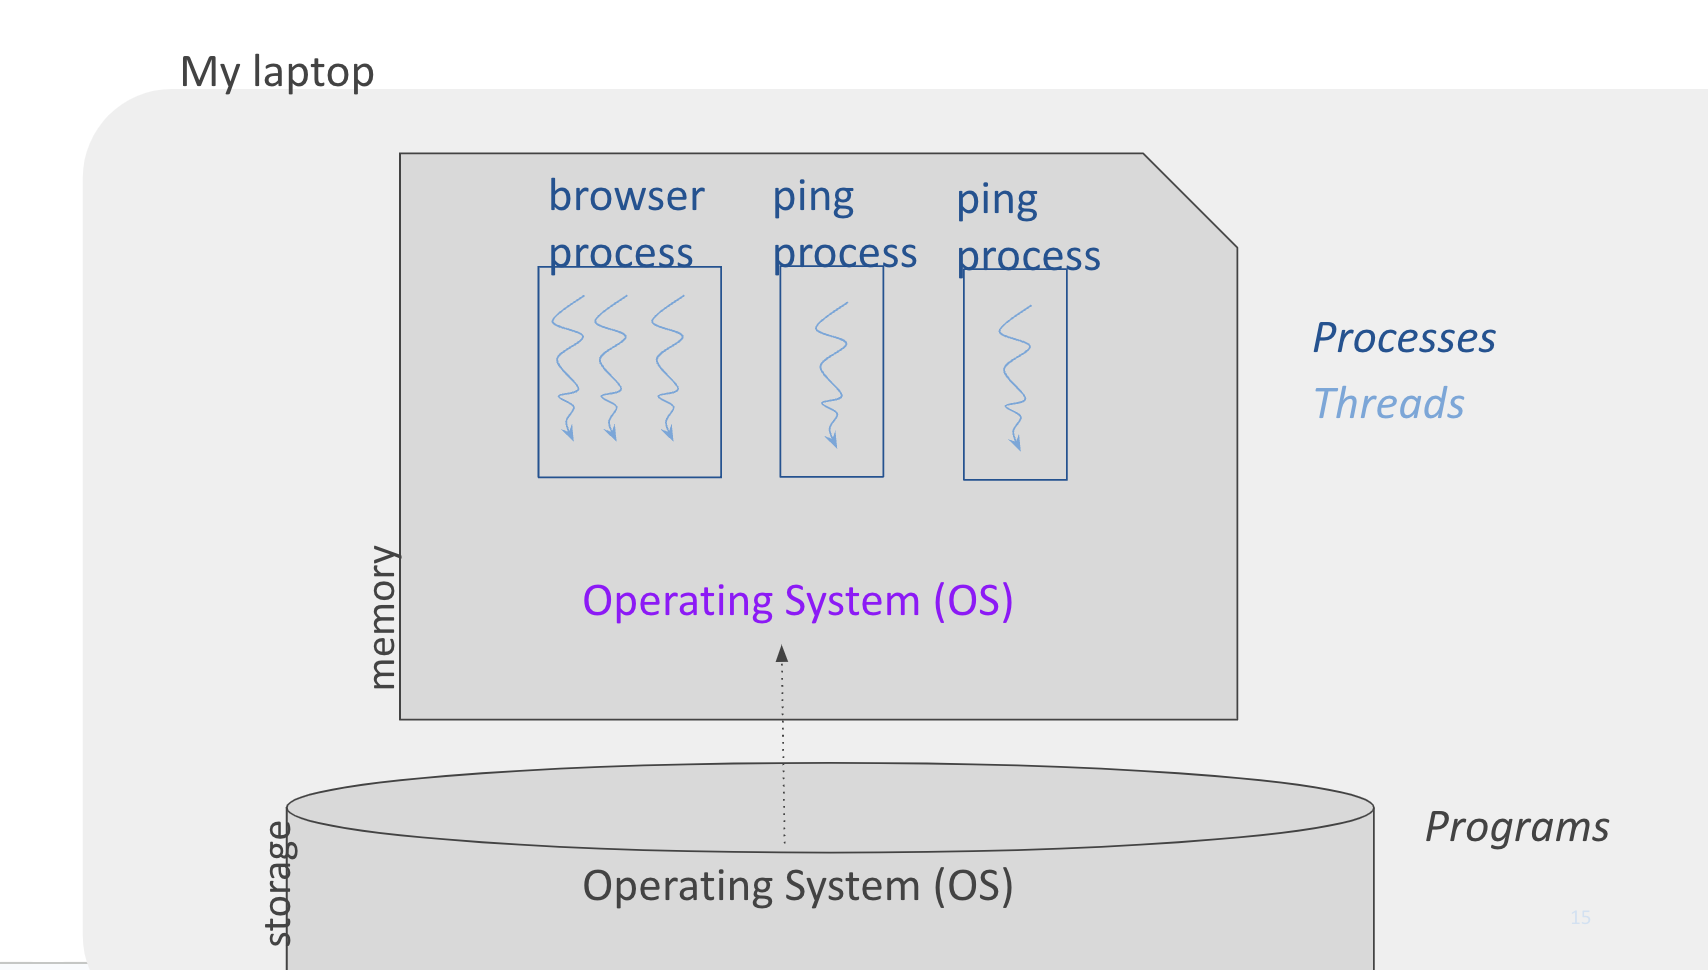
\includegraphics[width=1.15\textwidth]{chapters/L1/images/os.png}
\end{center}
\end{minipage}

\subsection{Example: Execution When Fetching a Video from YouTube}
When you click a YouTube link, the following sequence of events occurs:
\begin{enumerate}
  \item Your trackpad detects the click and notifies the OS.
  \item The OS identifies that the click occurred within the web browser window and alerts the corresponding process.
  \item The browser process initiates a chain of events that eventually fetches and displays the video.
\end{enumerate}

\begin{center}
  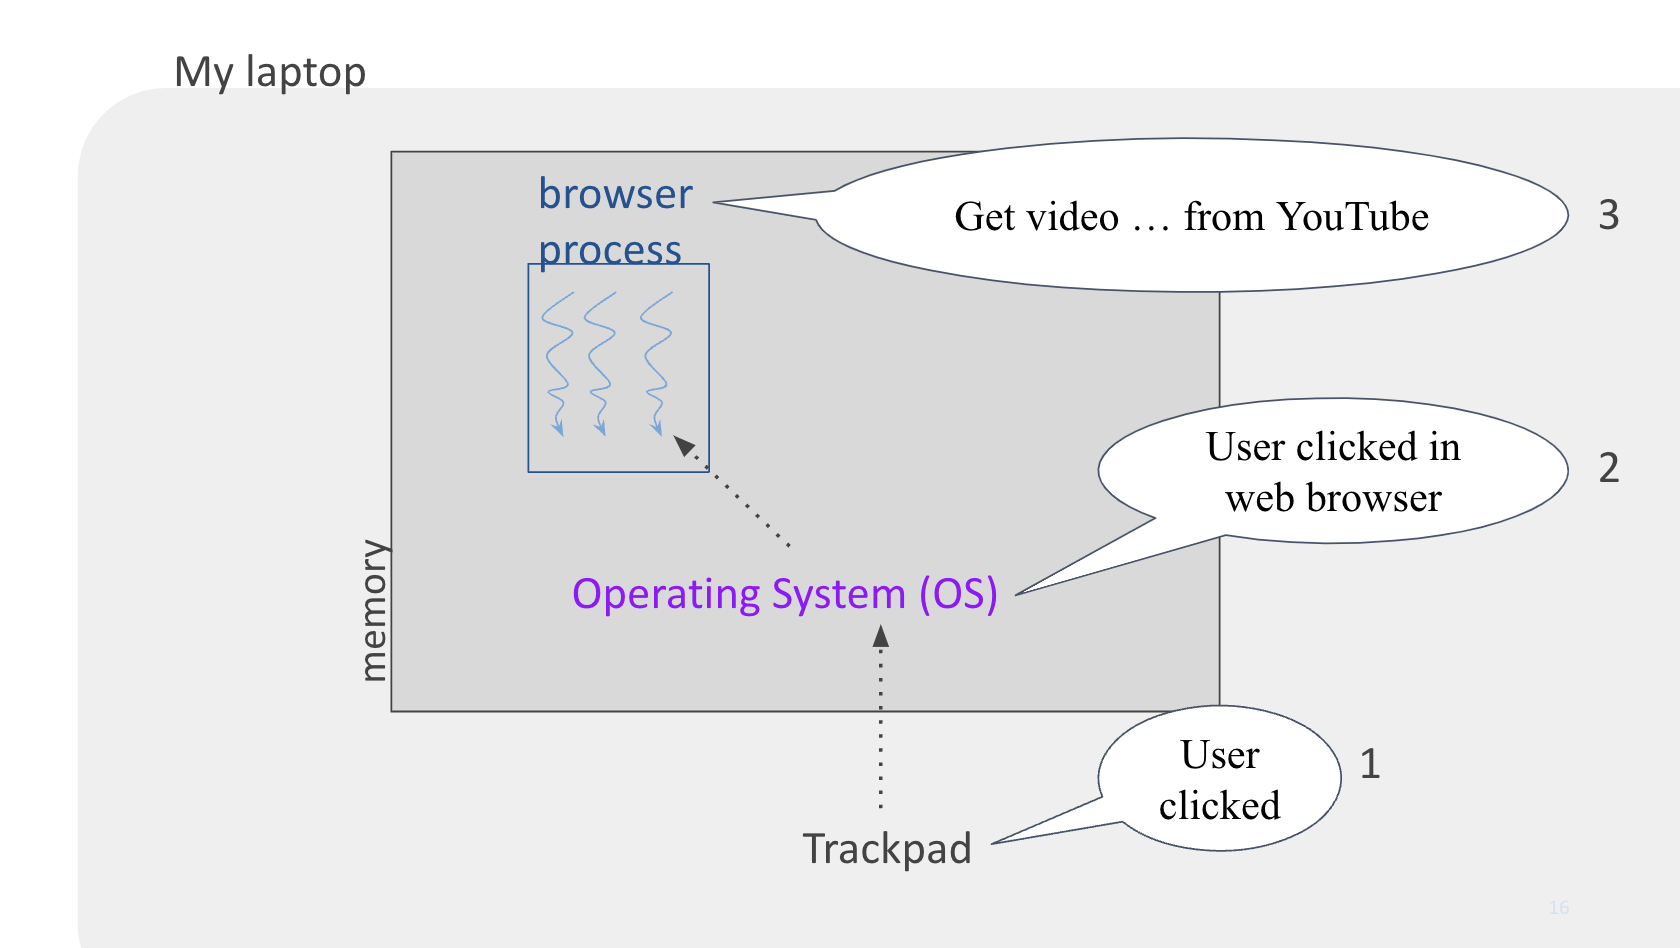
\includegraphics[width=0.85\textwidth]{chapters/L1/images/os_youtube.png}
\end{center}

\newpage
%%%%%%%%%%%%%%%%%%%%%%%%%%%%%%%%%%%%%%%%%%%%%%%%%%%%%%%%%%%%%%%%%%%%%%
\section{Program and ISA}
\subsection{Program}
A \textbf{program} is a set of instructions written by a human in a high-level programming language (such as C, Java, or Python) that implements an algorithm. When compiled, a program is translated into an \emph{executable} (or binary) that the CPU can run. The executable is expressed in the language defined by the computer's \textbf{Instruction Set Architecture} (ISA).

\begin{center}
  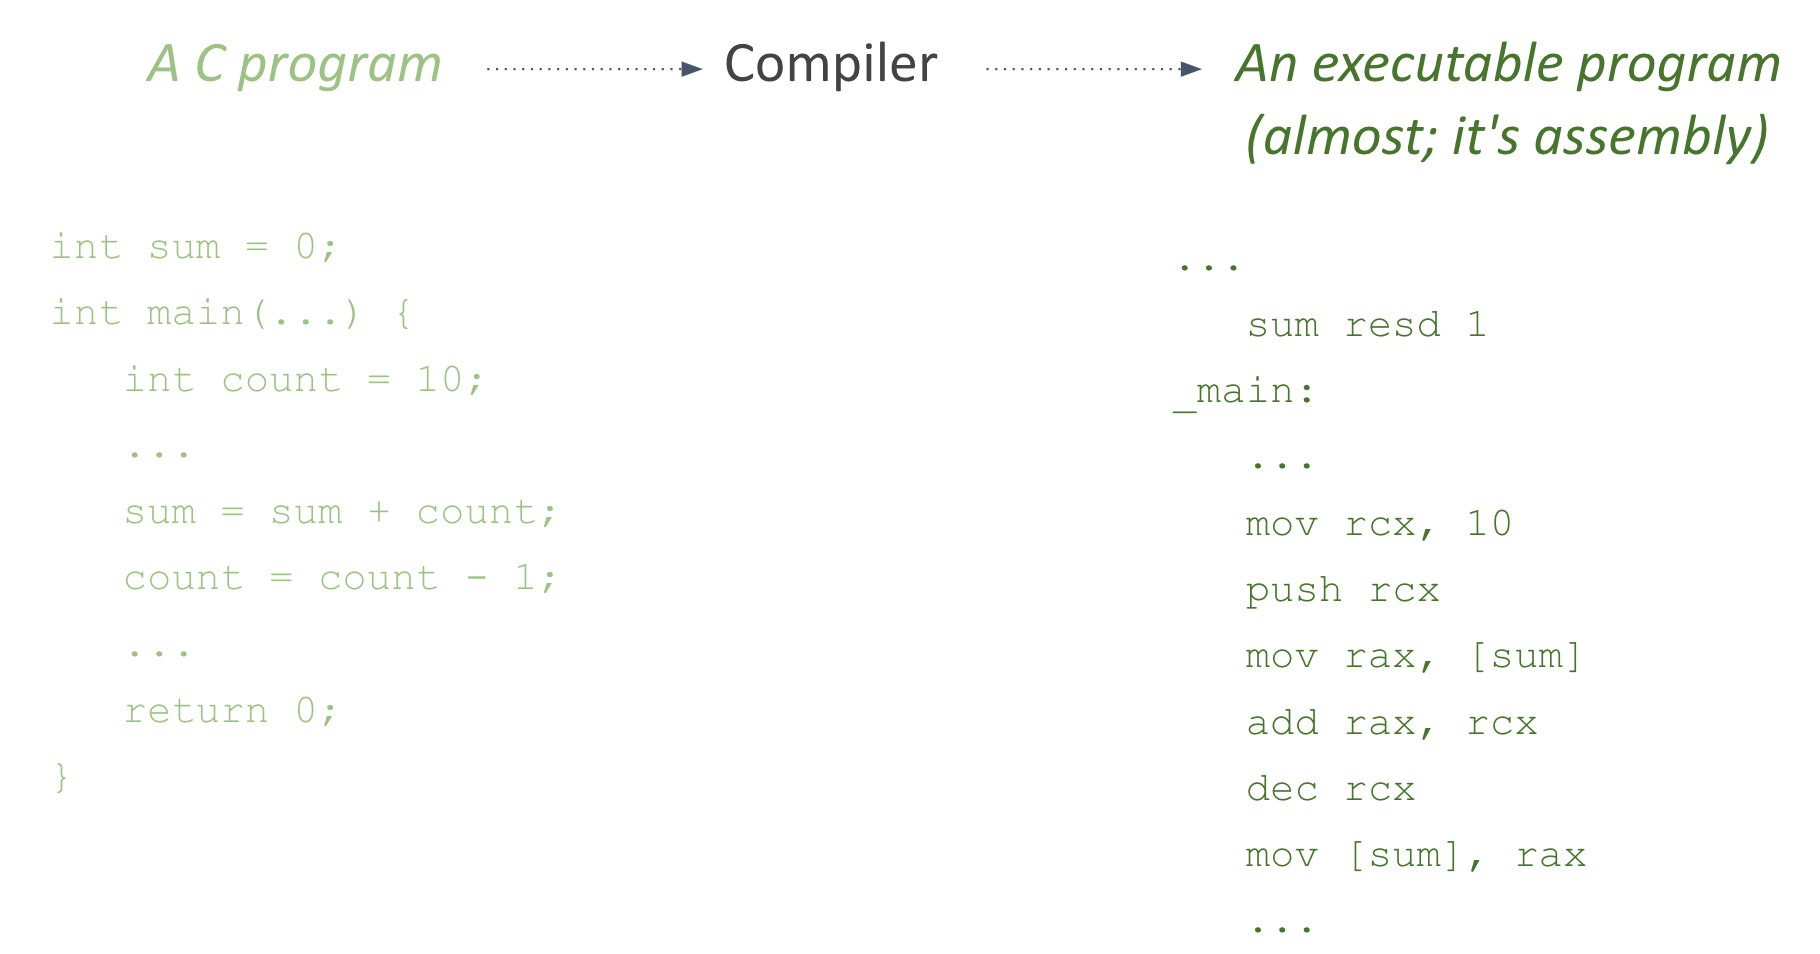
\includegraphics[width=0.75\textwidth]{chapters/L1/images/program.png}
\end{center}

\begin{minipage}{0.45\textwidth}
\begin{definition}[ISA]
The \textbf{Instruction Set Architecture} (ISA) is the set of all instructions that a CPU can understand and execute. It forms an interface between the compiler (which translates high-level code into machine code) and the CPU.
\end{definition}
\end{minipage}
\hfill
\vline
\hfill
\begin{minipage}{0.45\textwidth}
\begin{center}
  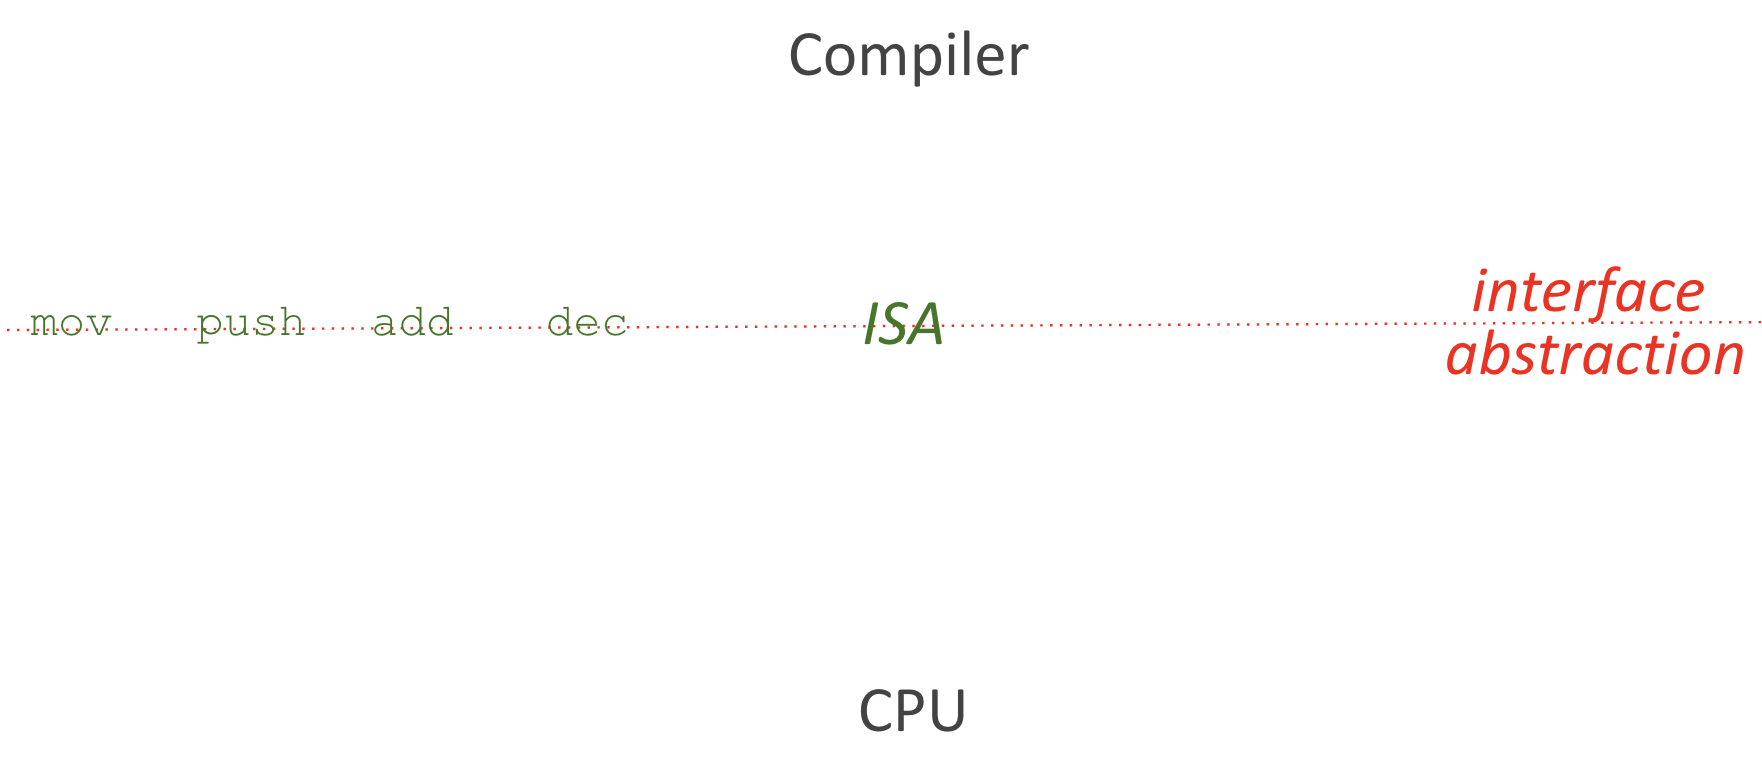
\includegraphics[width=1.25\textwidth]{chapters/L1/images/isa.png}
\end{center}
\end{minipage}\\
\vfill
\begin{definition}[Von Neumann Architecture]
The vast majority of computers today follow the \textbf{Von Neumann architecture}, which is characterized by a single main memory that holds both data and instructions.

\begin{center}
  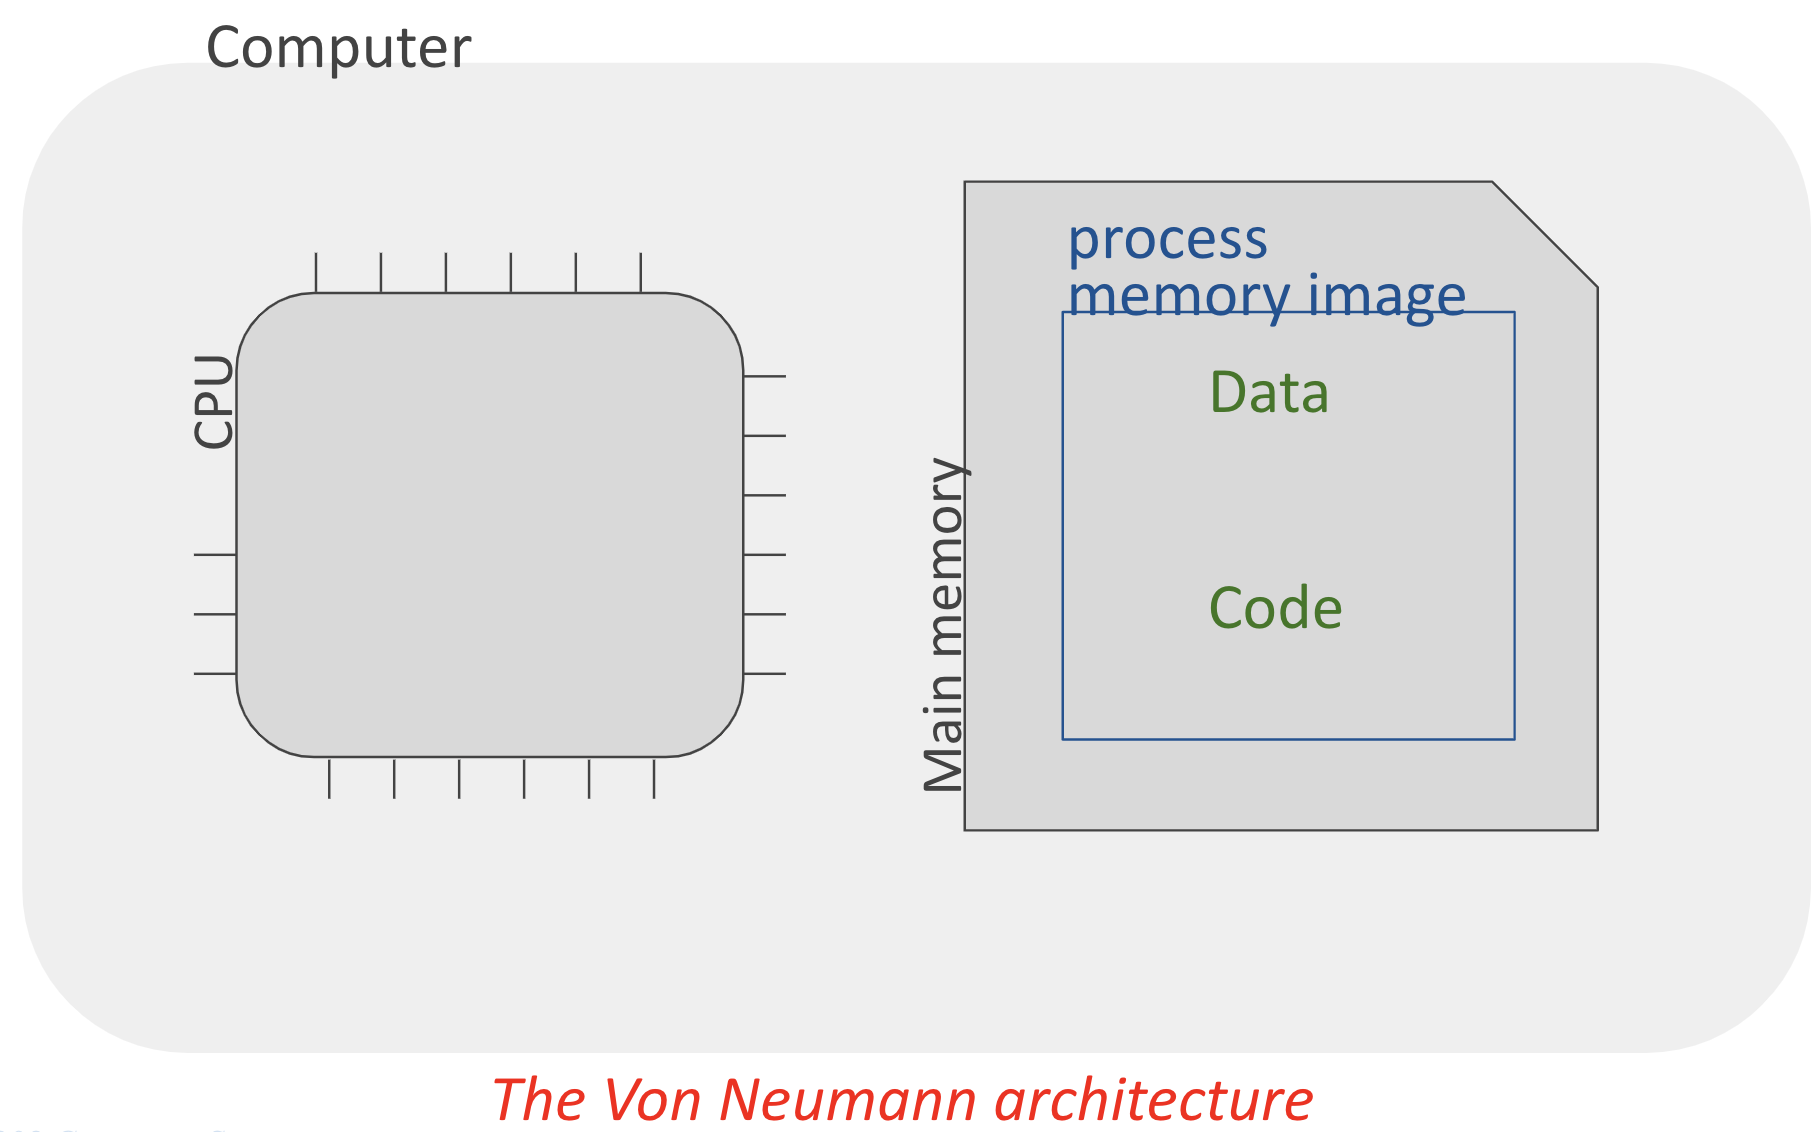
\includegraphics[width=0.55\textwidth]{chapters/L1/images/von.png}
\end{center}
\end{definition}

%%%%%%%%%%%%%%%%%%%%%%%%%%%%%%%%%%%%%%%%%%%%%%%%%%%%%%%%%%%%%%%%%%%%%%
\begin{definition}[CPU Frequency]
A CPU’s frequency indicates how many cycles it can perform in one second. For example, a 4.05~GHz CPU performs 4.05 billion cycles per second. In this context, a \textbf{cycle} is the minimum time needed for the CPU to complete an operation or for a result to become ready.\\
\vspace{0.5em}
{\textbf{Question:} What is the meaning of the Hz metric?}\\[0.5em]
\textbf{Answer:} Hertz (Hz) measures the number of cycles per second.
\vspace{0.5em}
{\textbf{Question:} In the context of a CPU, what is a cycle?}\\[0.5em]
\textbf{Answer:} A cycle is the minimum unit of time required for the CPU to produce a result from executing an instruction.
\end{definition}


%%%%%%%%%%%%%%%%%%%%%%%%%%%%%%%%%%%%%%%%%%%%%%%%%%%%%%%%%%%%%%%%%%%%%%
\section{Frequency Imbalance and CPU Caching}

Modern systems exhibit a \emph{frequency imbalance} between the CPU and main memory. While the CPU might complete an instruction in approximately 1~nsec, accessing data from DRAM typically takes 50–150~nsec. As a result, the CPU can spend a significant amount of time idle, waiting for data.

\begin{center}
  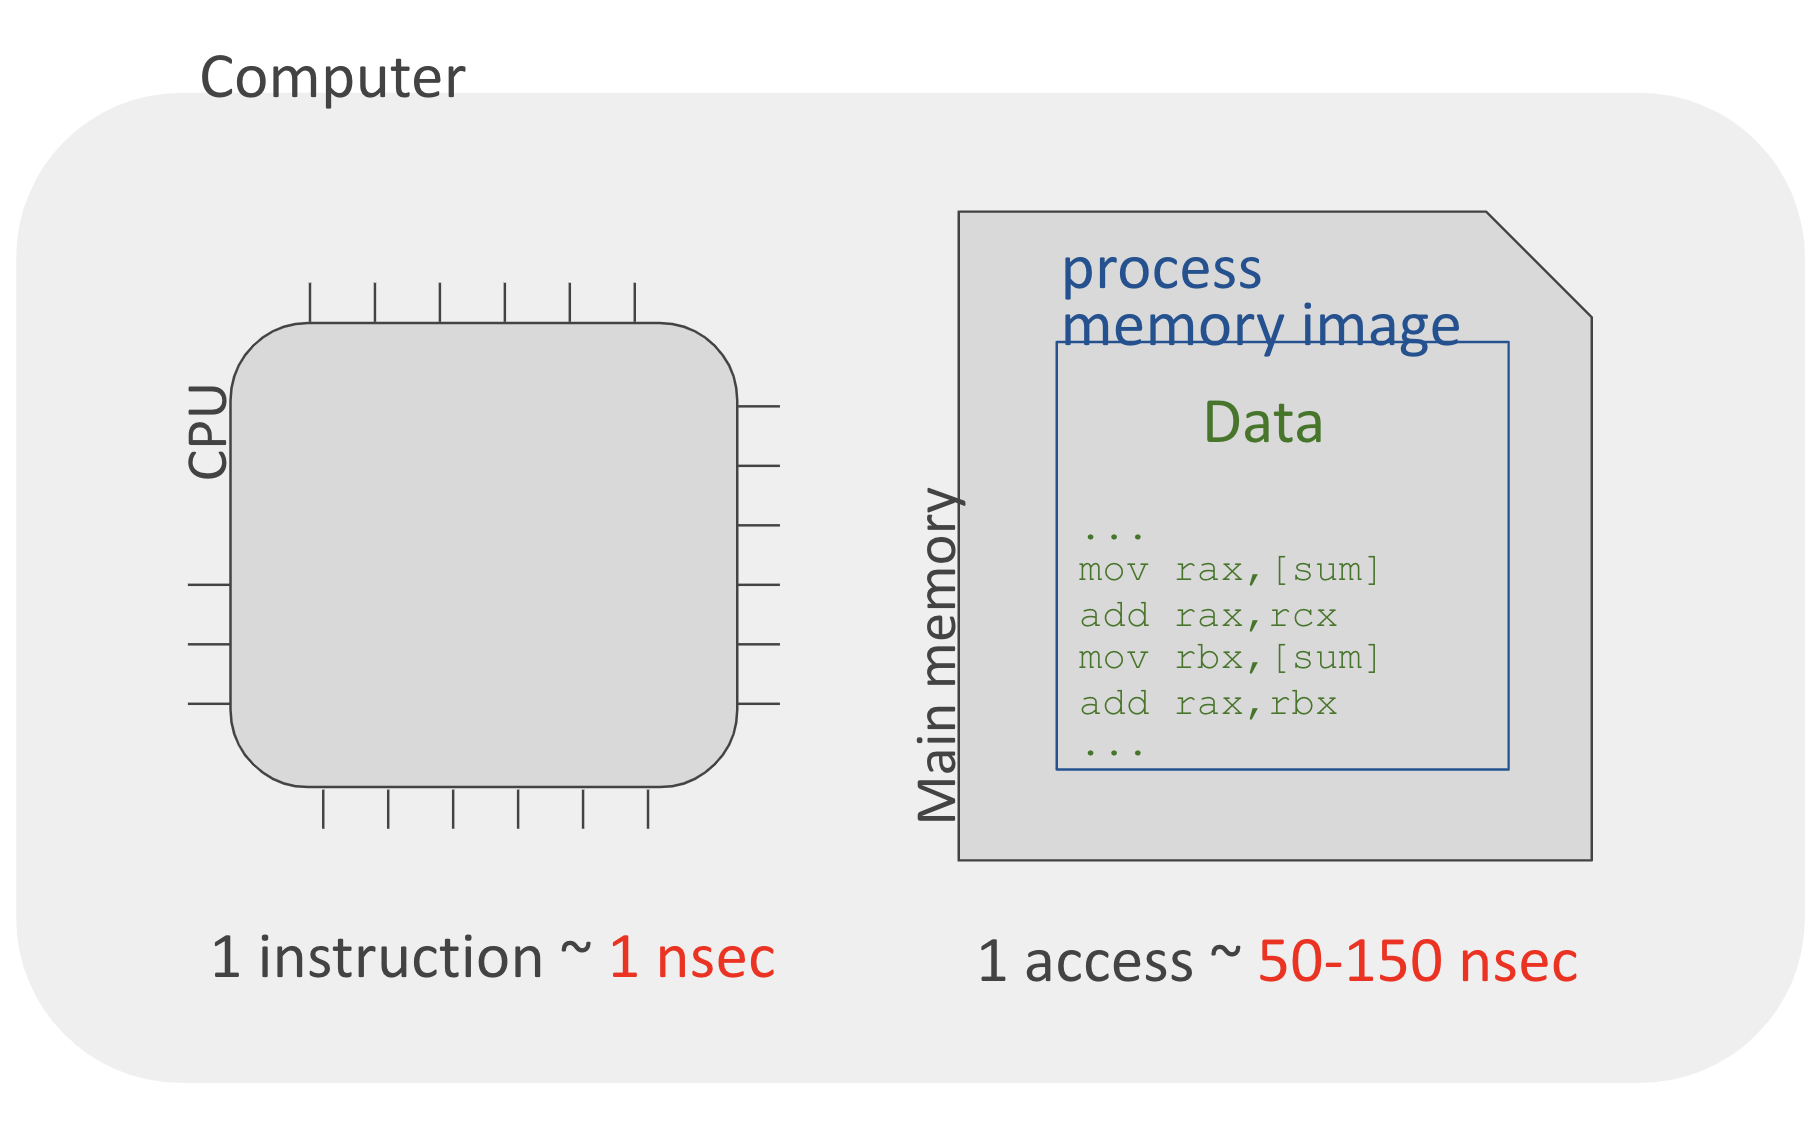
\includegraphics[width=0.65\textwidth]{chapters/L1/images/imbalance.png}
\end{center}

\vspace{0.5em}
{\textbf{Question:} How can we improve the efficiency of a system with such a frequency imbalance?}\\[0.5em]
\textbf{Answer:} We can improve efficiency by using caching. A small, fast memory (the CPU cache) stores recently accessed data so that subsequent accesses are much faster.
\newpage
\subsection{CPU Caching}
CPU caching adds a small amount of high-speed memory inside the CPU. When data is requested, the cache is checked first. If the data is already in the cache (a cache hit), the CPU retrieves it quickly. Otherwise (a cache miss), the data is fetched from the slower main memory and stored in the cache for future accesses.

\begin{center}
  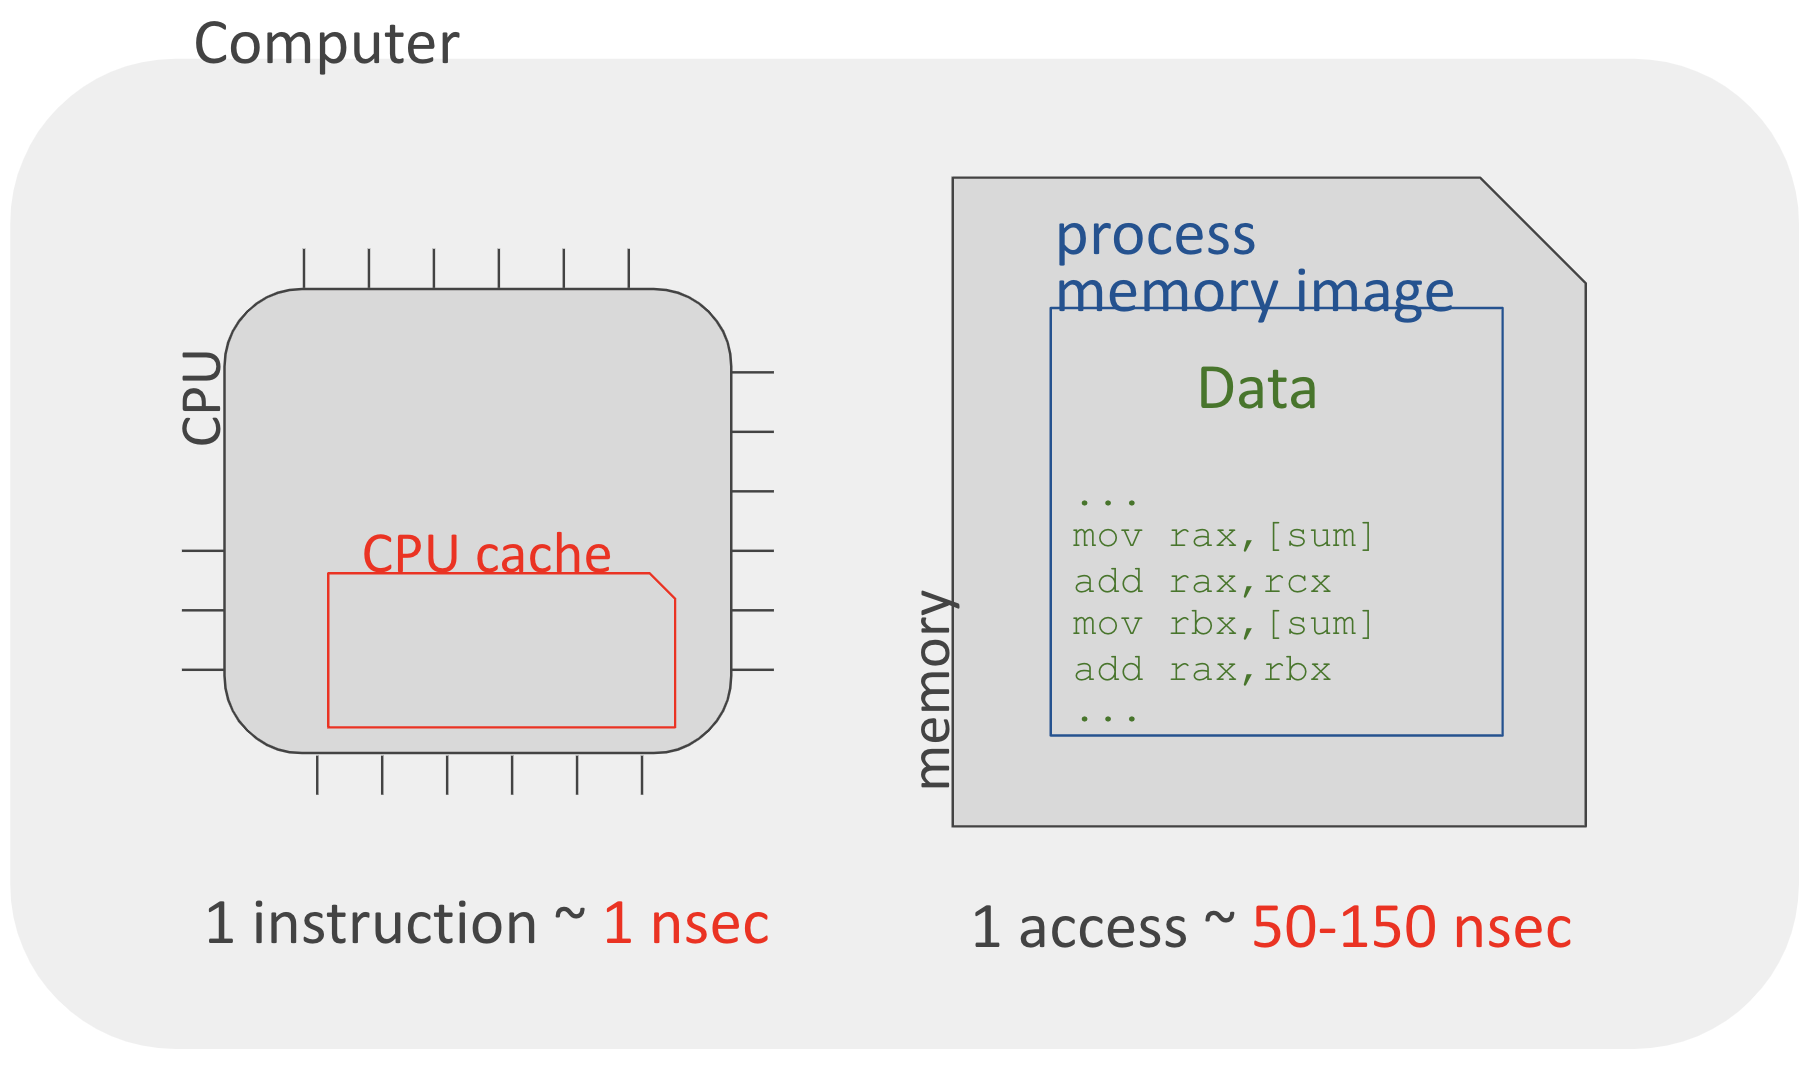
\includegraphics[width=0.65\textwidth]{chapters/L1/images/cache.png}
\end{center}

%%%%%%%%%%%%%%%%%%%%%%%%%%%%%%%%%%%%%%%%%%%%%%%%%%%%%%%%%%%%%%%%%%%%%%
\section{Memory Accesses vs. I/O}

\subsection{Memory Accesses}
When a process reads or writes data in main memory, it uses fast CPU instructions (load/store). These operations are efficient and do not interrupt the normal flow of the process.

\subsection{Back to YouTube Fetching: System Calls in Action}

Returning to our YouTube example, when the browser process calls a \texttt{send} syscall to request a video, the CPU stops executing the browser’s code and switches to executing the more privileged code in the OS. This is because accessing external resources (network or storage) requires a syscall.

\begin{center}
  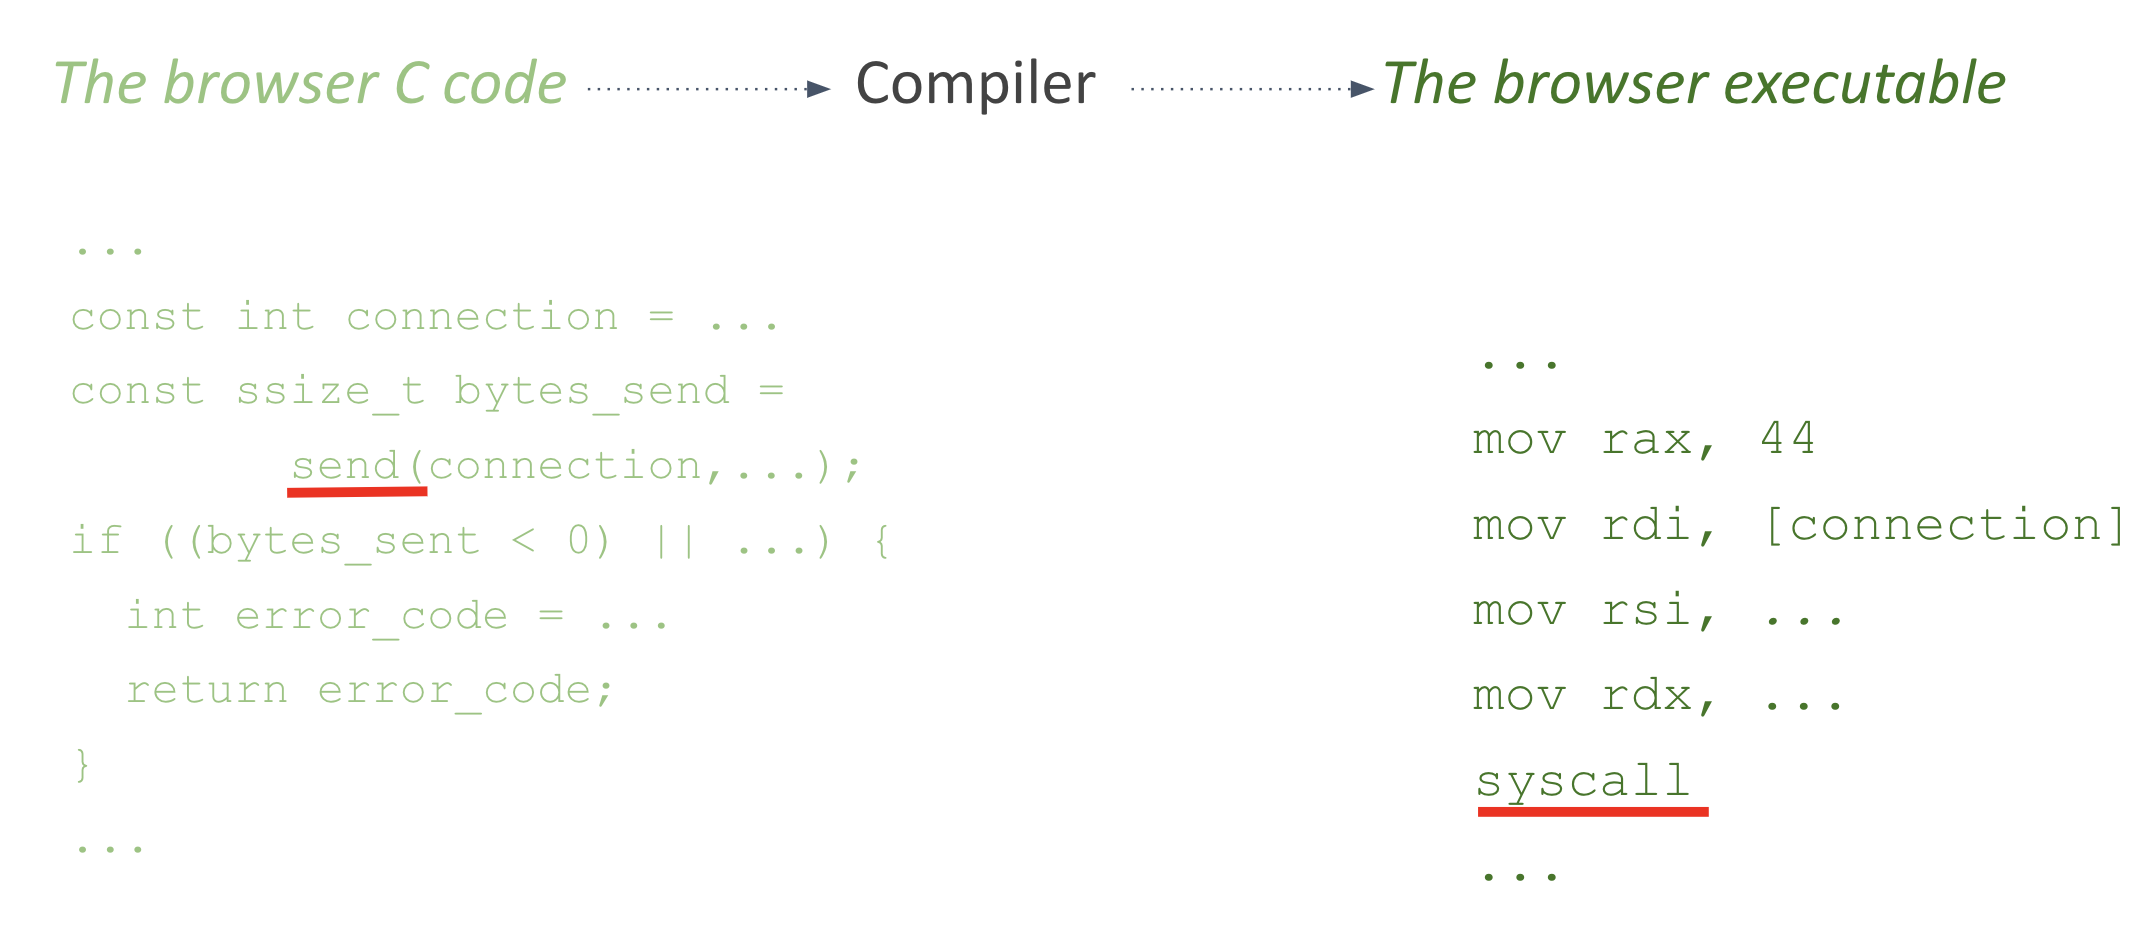
\includegraphics[width=0.85\textwidth]{chapters/L1/images/syscalls2.png}
\end{center}
\newpage
\subsection{Mixing Interfaces}
When a process makes a syscall for network communication (such as \texttt{send} or \texttt{recv}), the CPU transitions from running the process’s code to running the OS code associated with the network stack. This is an example of mixing different interfaces: the process interface (its own code) and the OS interface (syscalls).
\begin{center}
  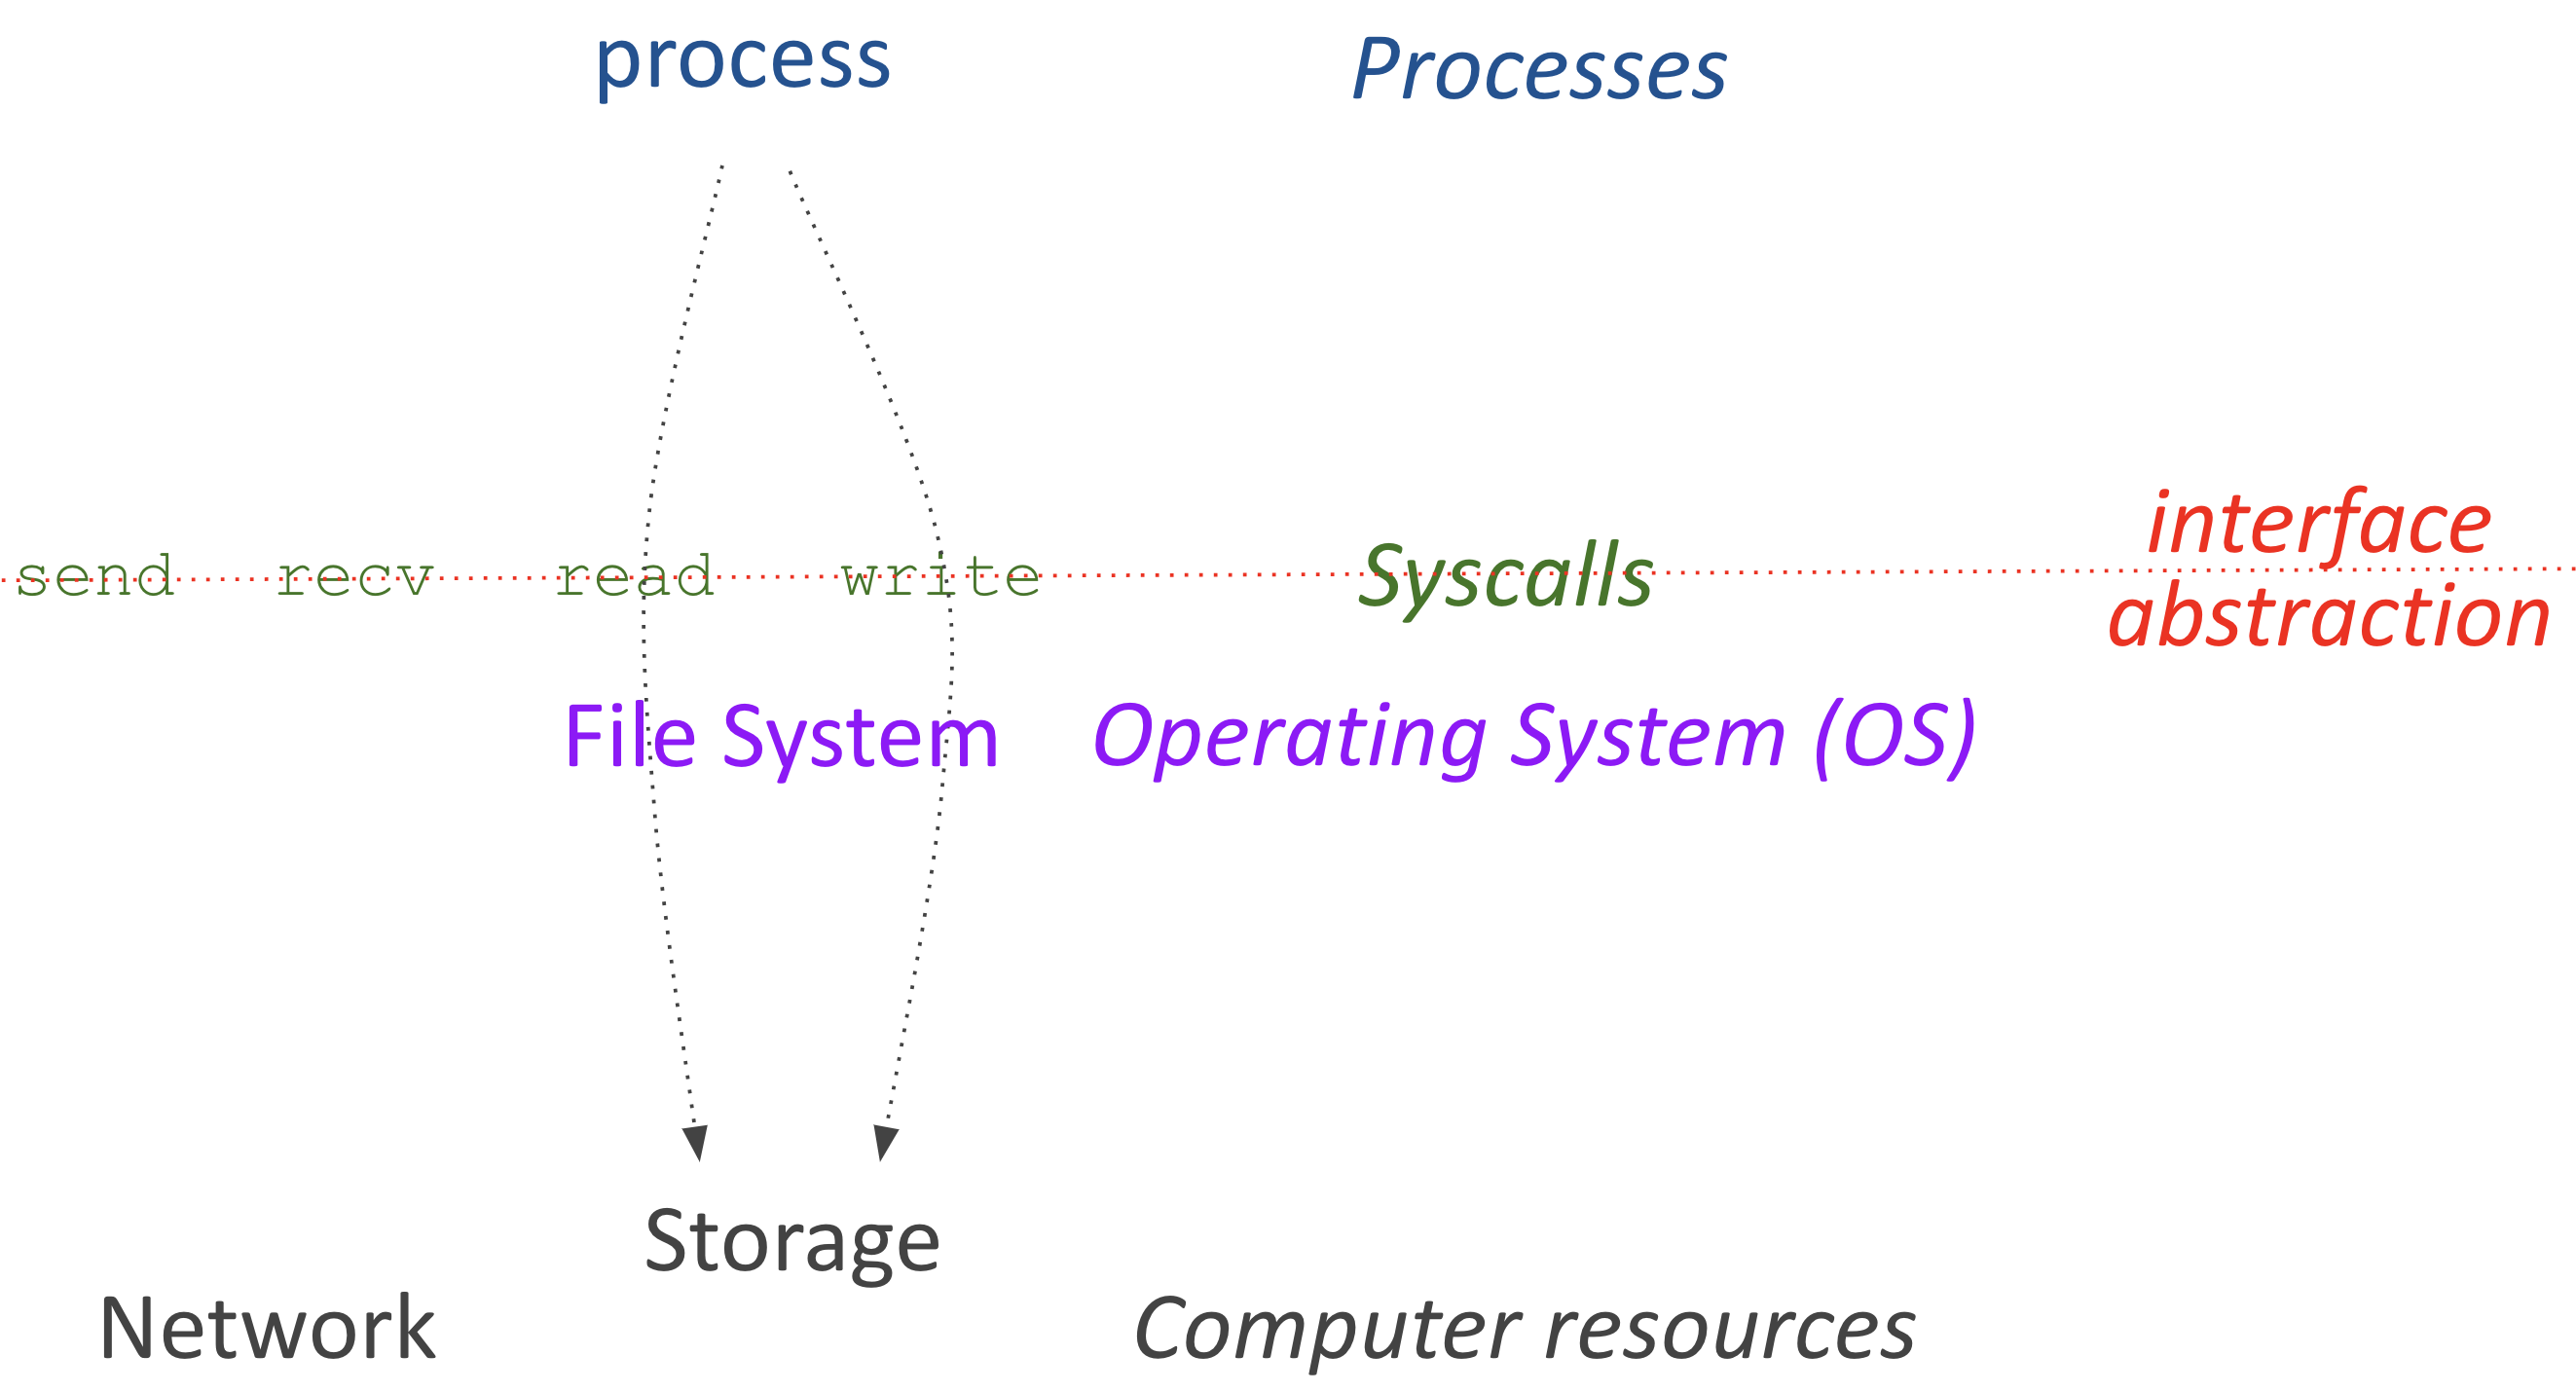
\includegraphics[width=0.65\textwidth]{chapters/L1/images/mix_int.png}
\end{center}
\vfill
\begin{definition}[Memory Access and I/O]
\textbf{Memory Access} refers to the CPU’s direct read/write operations using load/store instructions in main memory. In contrast, \textbf{I/O (Input/Output)} involves accessing external devices (such as storage or network) via system calls. I/O operations are generally more expensive because they require the CPU to switch context to execute privileged OS code.
\end{definition}
\vspace{0.5em}
\textbf{Exam Question:} How is reading from main memory different from reading from storage or the network? \\[0.5em]
\textbf{Answer:} Reading from main memory uses direct CPU instructions (load/store) and is very fast (tens to hundreds of nanoseconds), whereas reading from storage or the network requires a syscall, which interrupts the process and involves additional overhead (microseconds to milliseconds).
\vfill
\begin{definition}[I/O]
\textbf{I/O} (Input/Output) refers to operations that allow a process to access resources outside of its immediate control, such as storage devices or the network, via system calls. I/O operations are generally slower than direct memory accesses.
\end{definition}
\vspace{0.5em}
\textbf{Exam Question:} If a program does not create or manipulate any data, will executing this program require reading anything from memory?\\[0.5em]
\textbf{Answer:} Yes, executing the program will still require reading something from memory. Even if the program does not create or manipulate any data, the CPU must at least fetch the instructions of the program itself from memory

\newpage
%%%%%%%%%%%%%%%%%%%%%%%%%%%%%%%%%%%%%%%%%%%%%%%%%%%%%%%%%%%%%%%%%%%%%%
\vfill
\section{Communication Over the Internet}
Internet communication involves transferring data over a network where different latencies are encountered: \\
\begin{minipage}{0.45\textwidth}
  \begin{itemize}
    \item[-] Simple CPU instructions: \(\sim\)1~nsec.
    \item[-] Main memory accesses: tens to hundreds of nanoseconds.
    \item[-] Reading 1~KB from an SSD: tens to hundreds of microseconds.
    \item[-] Requesting data over the Internet: several to hundreds of milliseconds.
\end{itemize}
\end{minipage}
\hfill
\vline
\hfill
\begin{minipage}{0.45\textwidth}
\begin{center}
  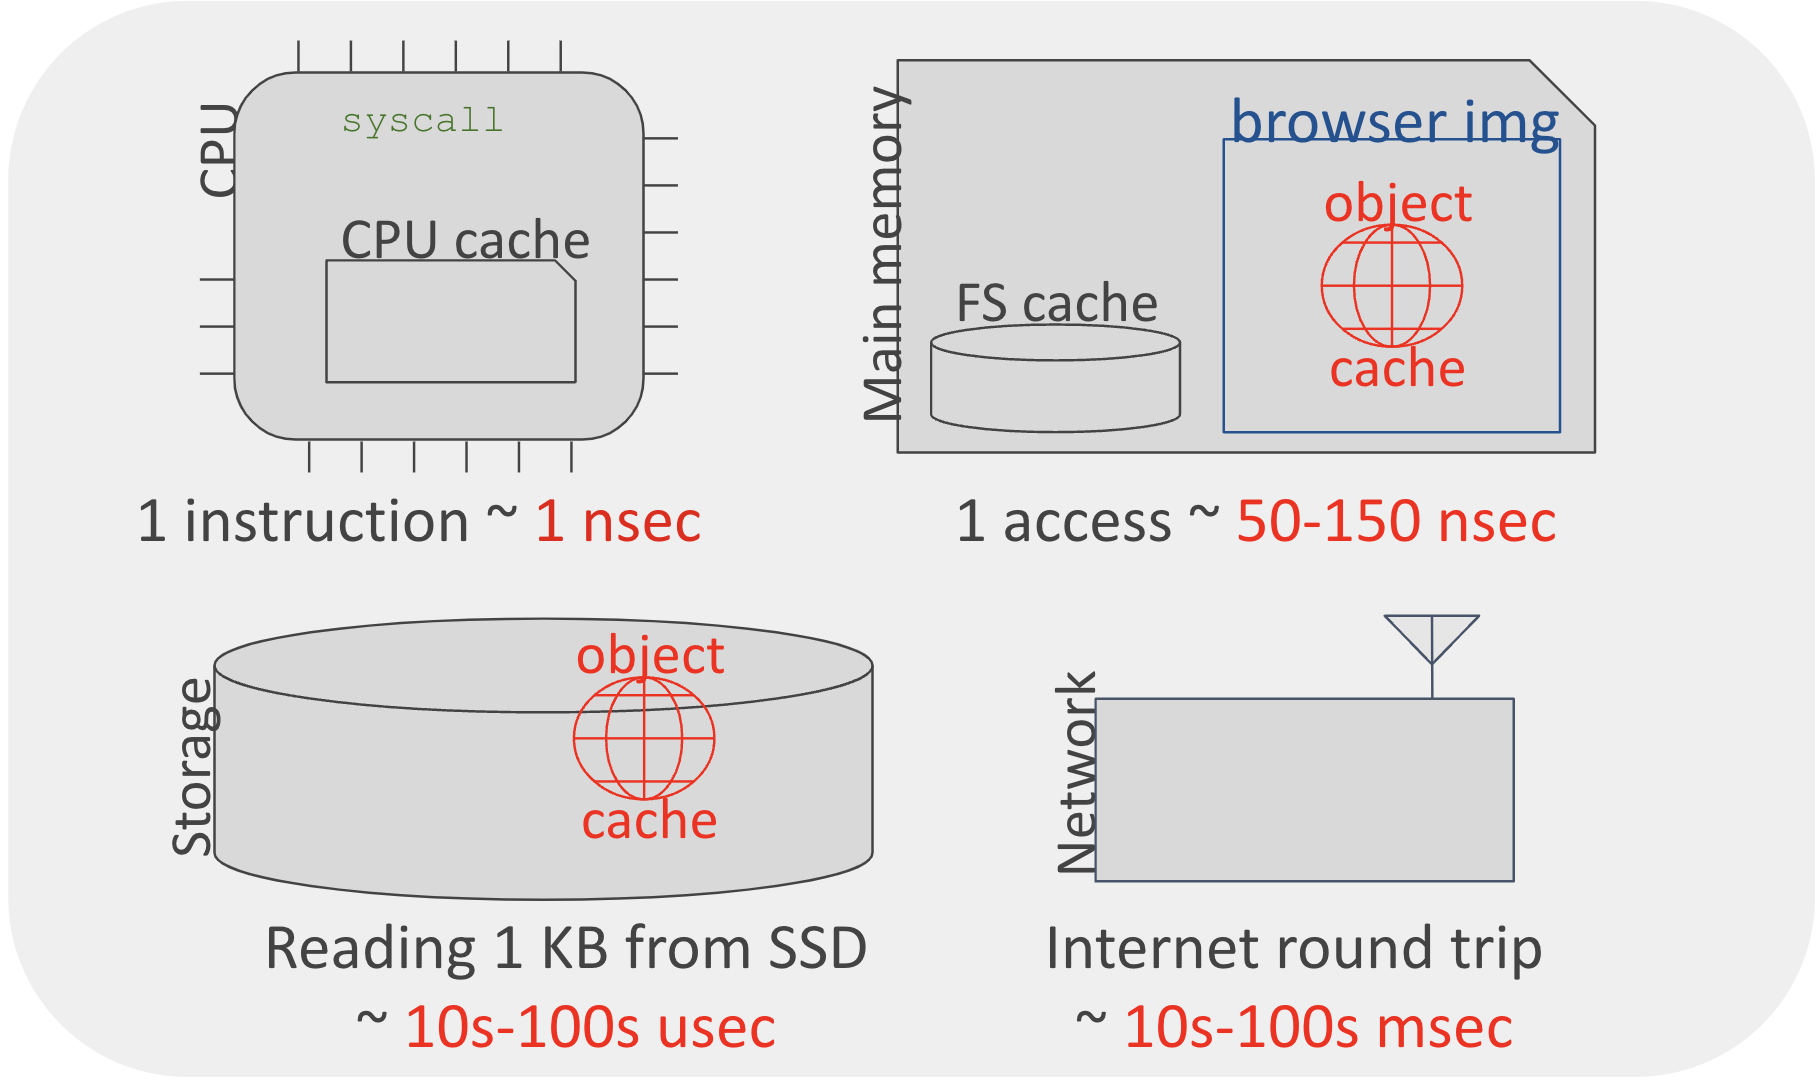
\includegraphics[width=1.15\textwidth]{chapters/L1/images/internet.png}
\end{center}
\end{minipage}\\[5px]
These delays make network communication expensive in terms of time, which is why caching is critical.
\vfill
%%%%%%%%%%%%%%%%%%%%%%%%%%%%%%%%%%%%%%%%%%%%%%%%%%%%%%%%%%%%%%%%%%%%%%
\subsection{End Systems}

The Internet is composed of \textbf{end systems}—devices that use the network for communication. These include laptops, smartphones, household appliances, connected cars, and even medical devices, as well as large cloud servers.

\begin{center}
  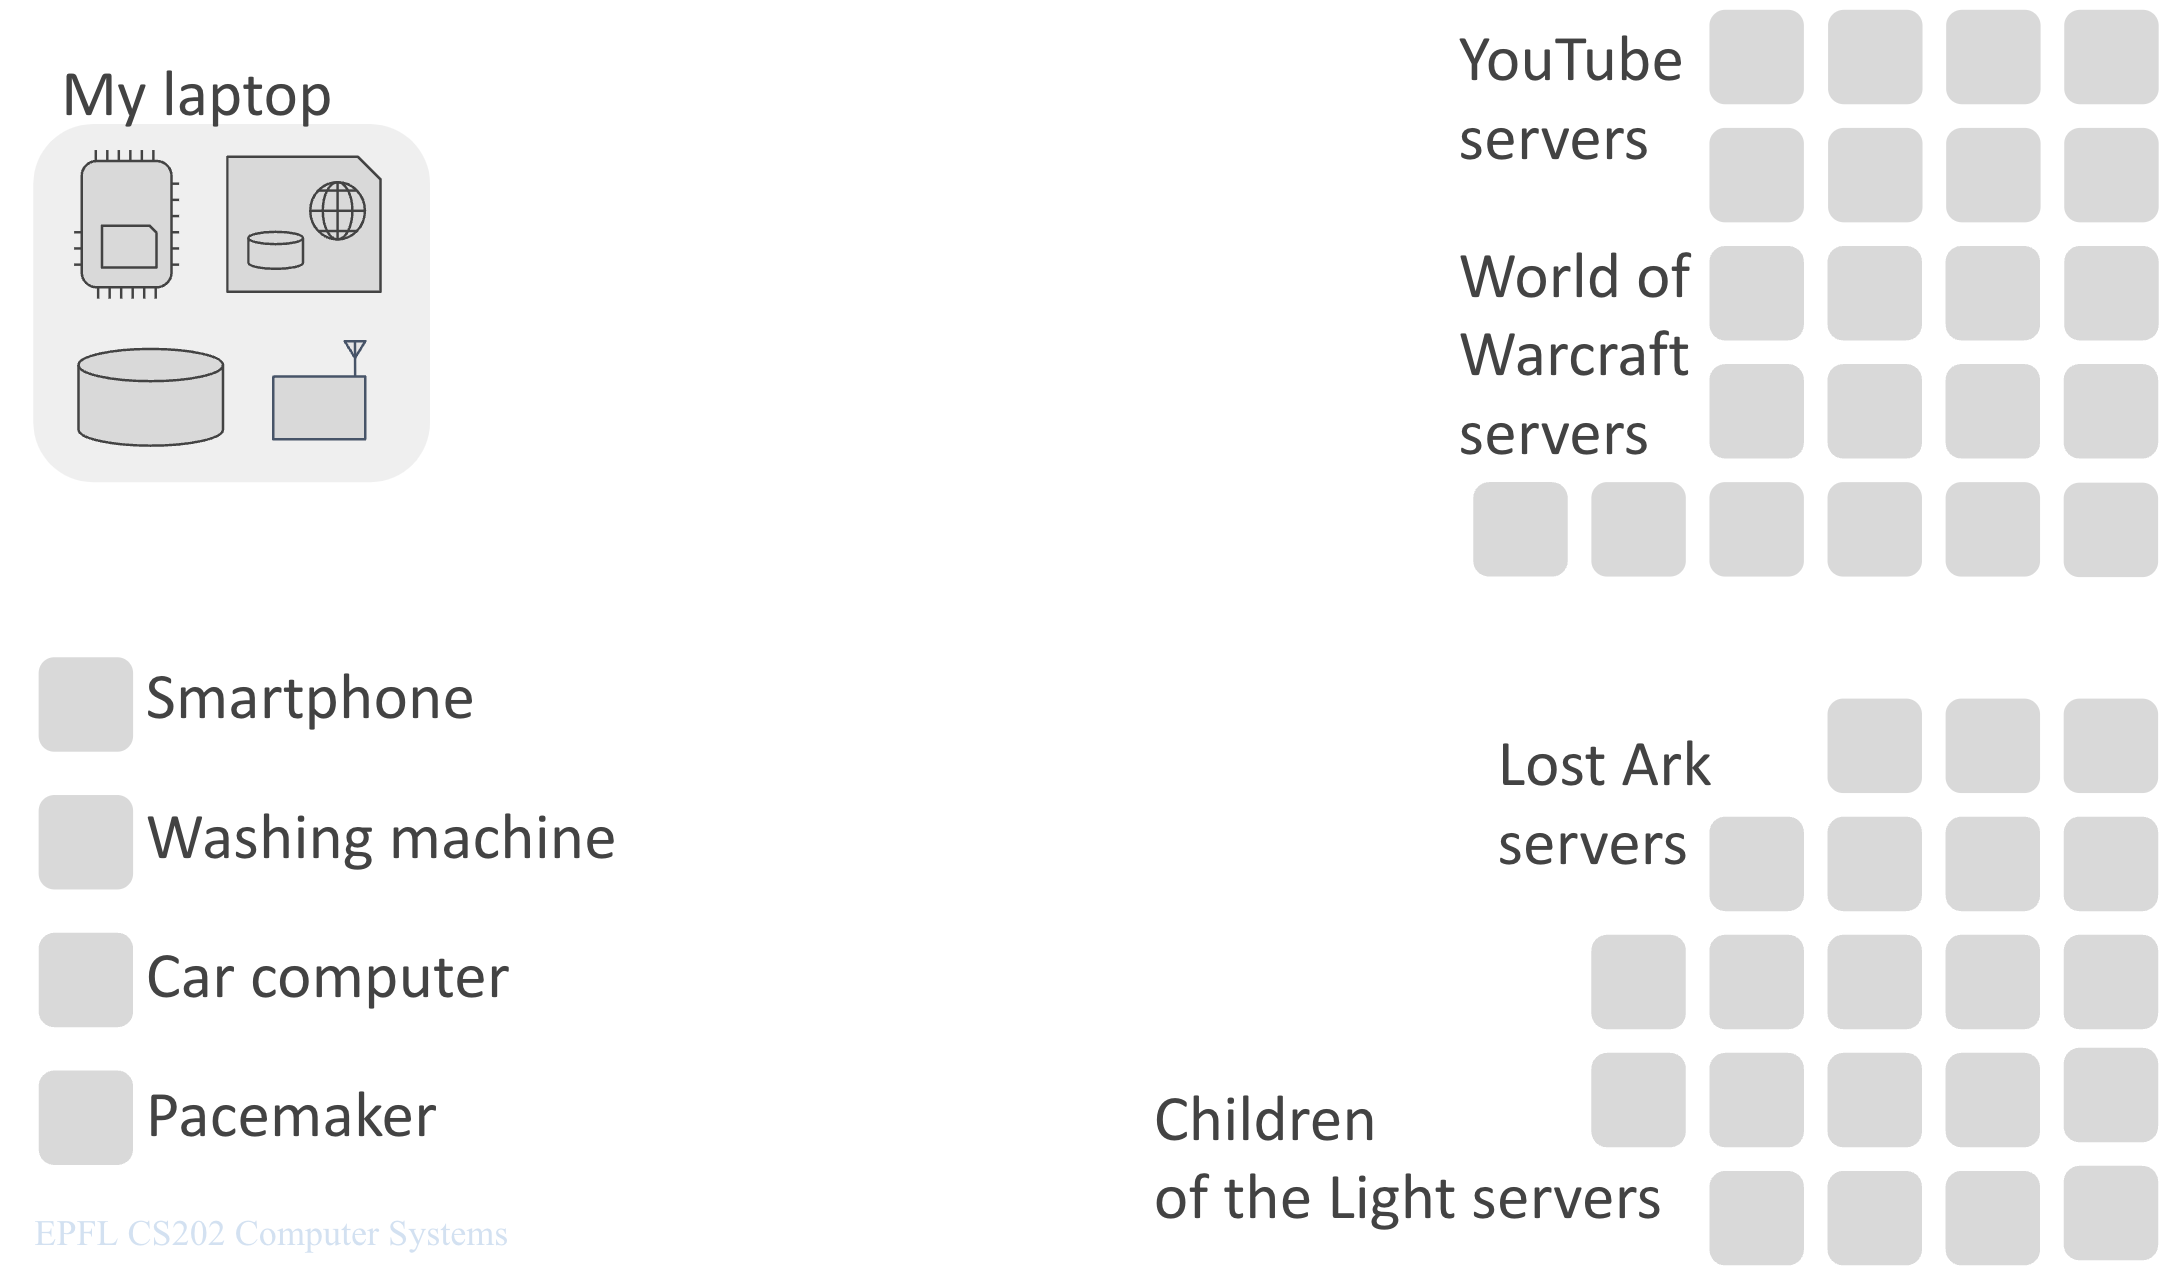
\includegraphics[width=0.65\textwidth]{chapters/L1/images/endsys.png}
\end{center}
\vfill
\newpage
%%%%%%%%%%%%%%%%%%%%%%%%%%%%%%%%%%%%%%%%%%%%%%%%%%%%%%%%%%%%%%%%%%%%%%
\subsection{Packet Switches and Network Links}

In addition to end systems, the Internet relies on:
\begin{itemize}
  \item[-] \textbf{Packet Switches}: Devices that route data between end systems.
  \item[-] \textbf{Network Links}: Physical connections that interconnect packet switches and end systems.
\end{itemize}

These components are managed by Internet Service Providers (ISPs) as well as major cloud providers.

\begin{center}
  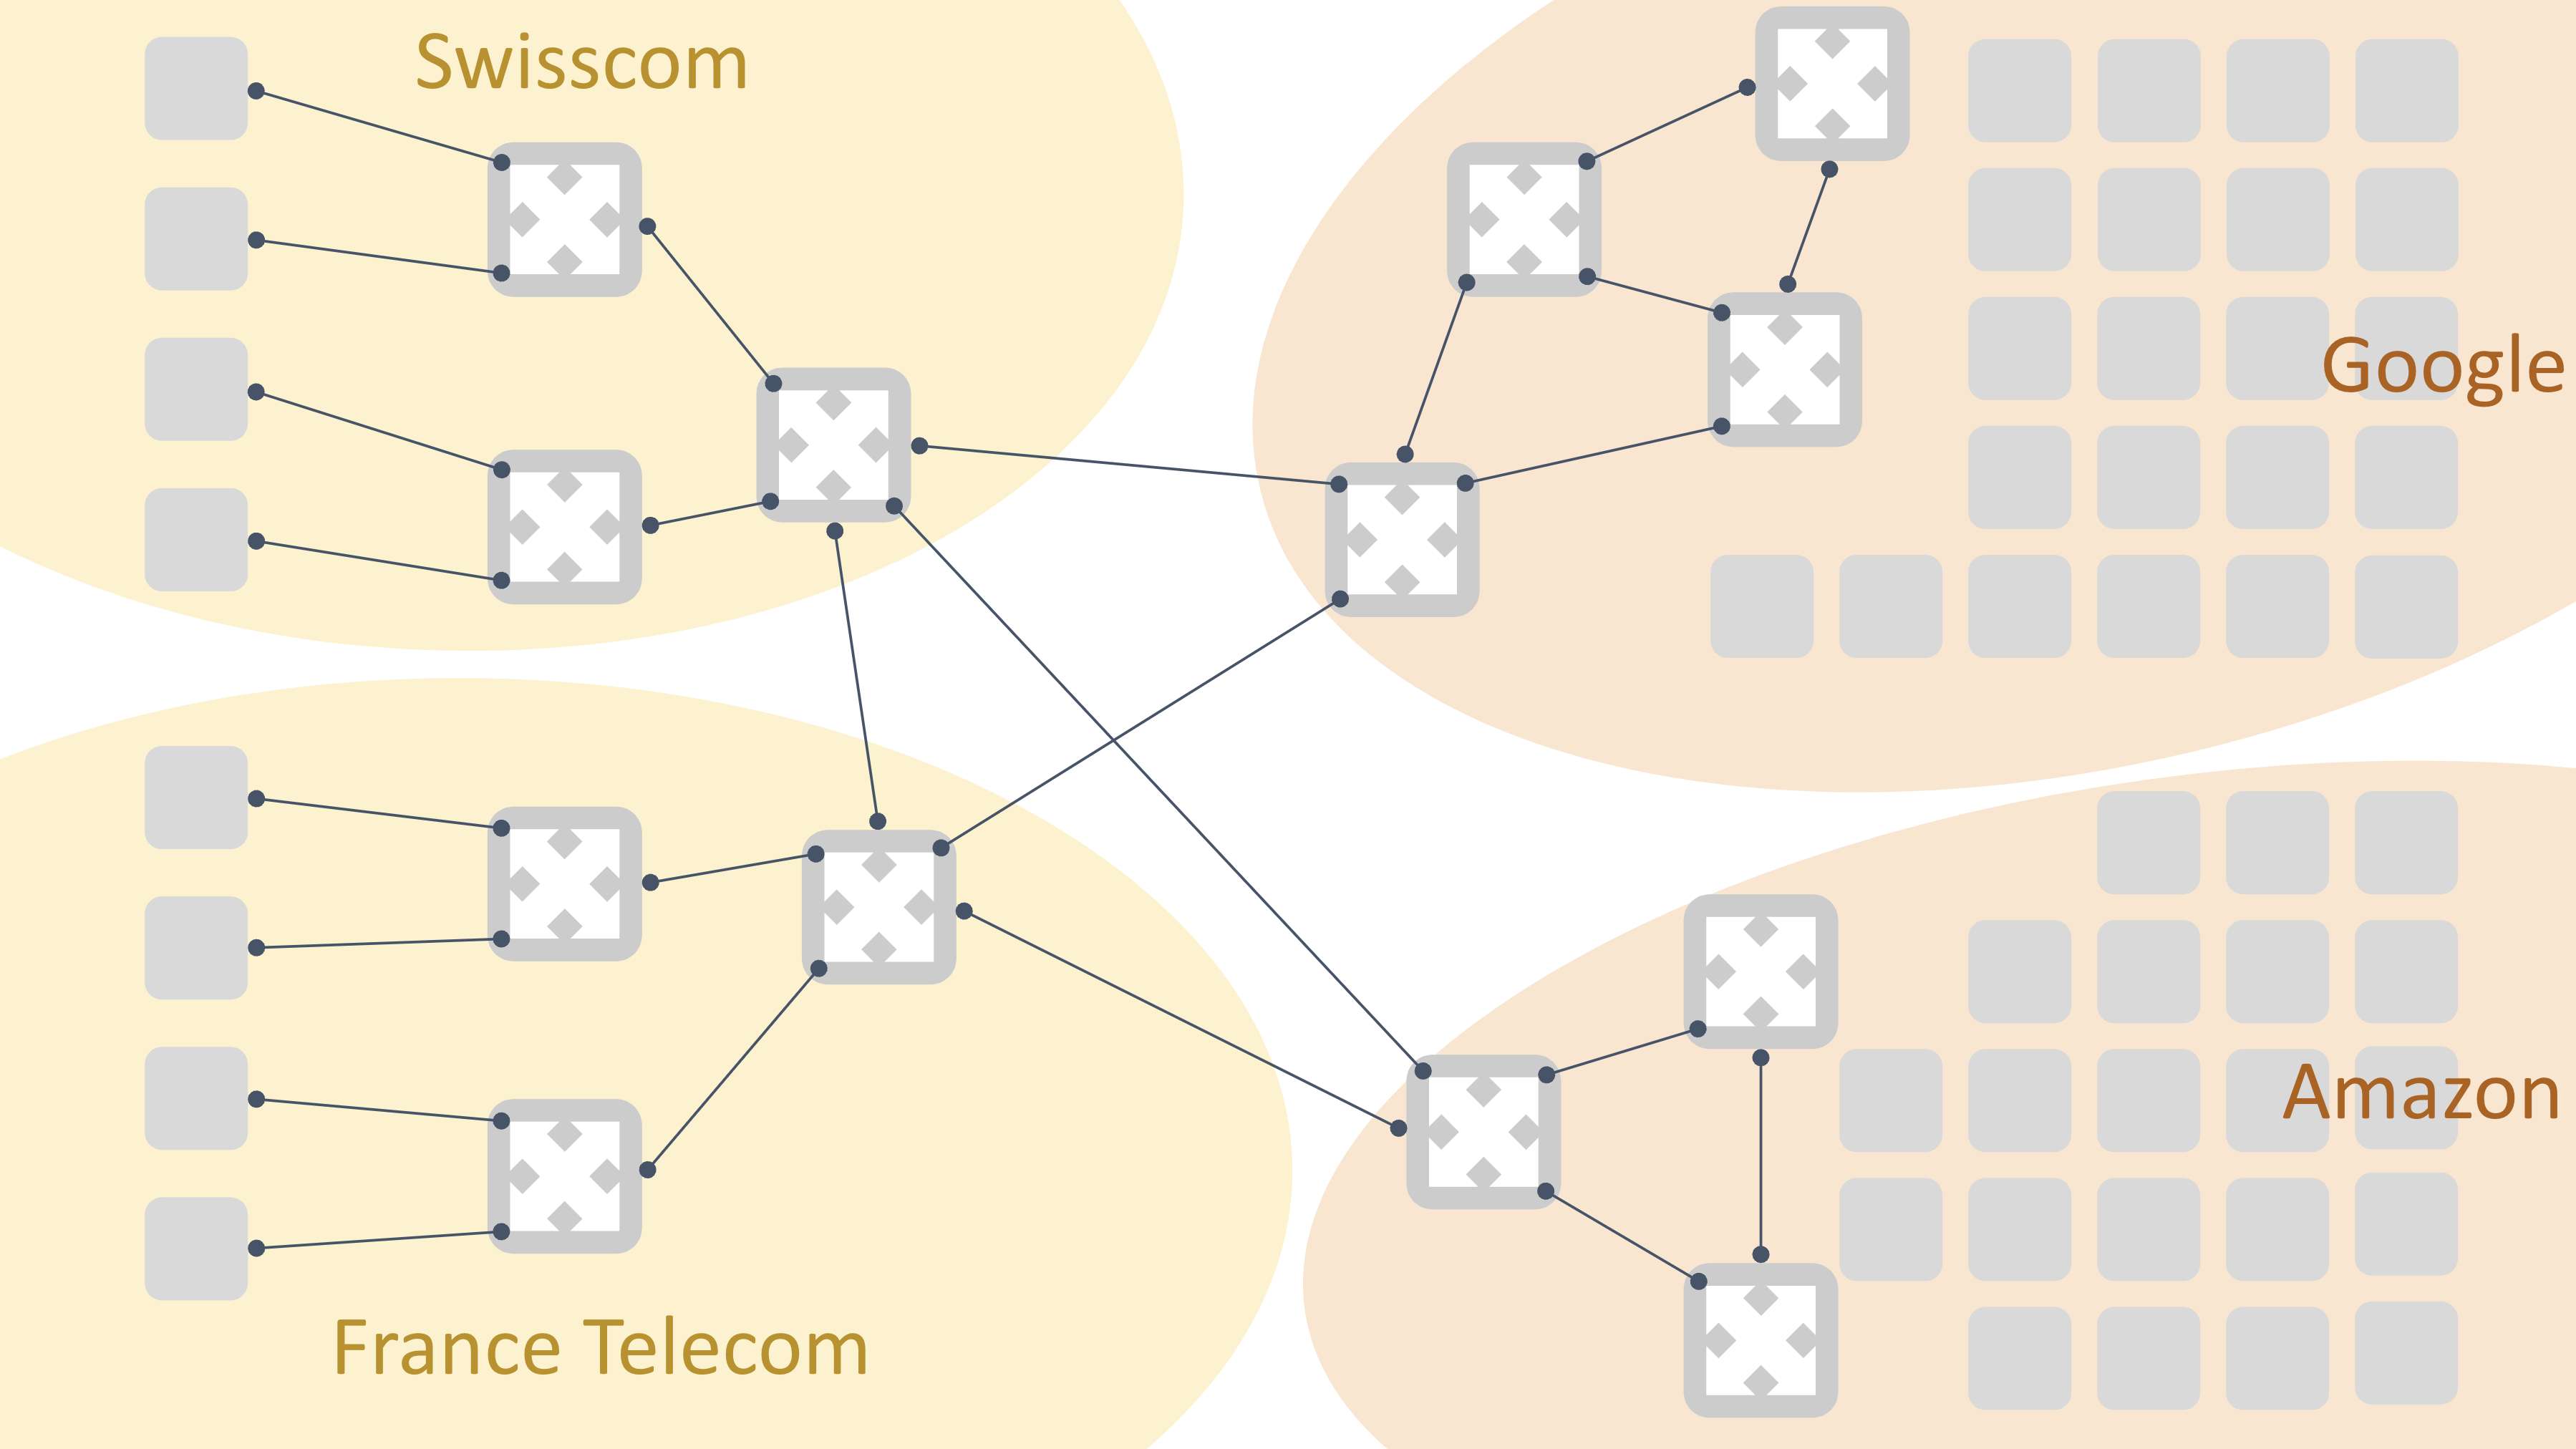
\includegraphics[width=0.65\textwidth]{chapters/L1/images/internet_schema.png}
\end{center}

%%%%%%%%%%%%%%%%%%%%%%%%%%%%%%%%%%%%%%%%%%%%%%%%%%%%%%%%%%%%%%%%%%%%%%
\subsection{Edge Caches}
To reduce the load on cloud data centers and improve user performance, large cloud providers often deploy \textbf{edge caches} within ISP networks. These caches store frequently accessed content closer to the end-users, reducing latency and network traffic.
\begin{center}
  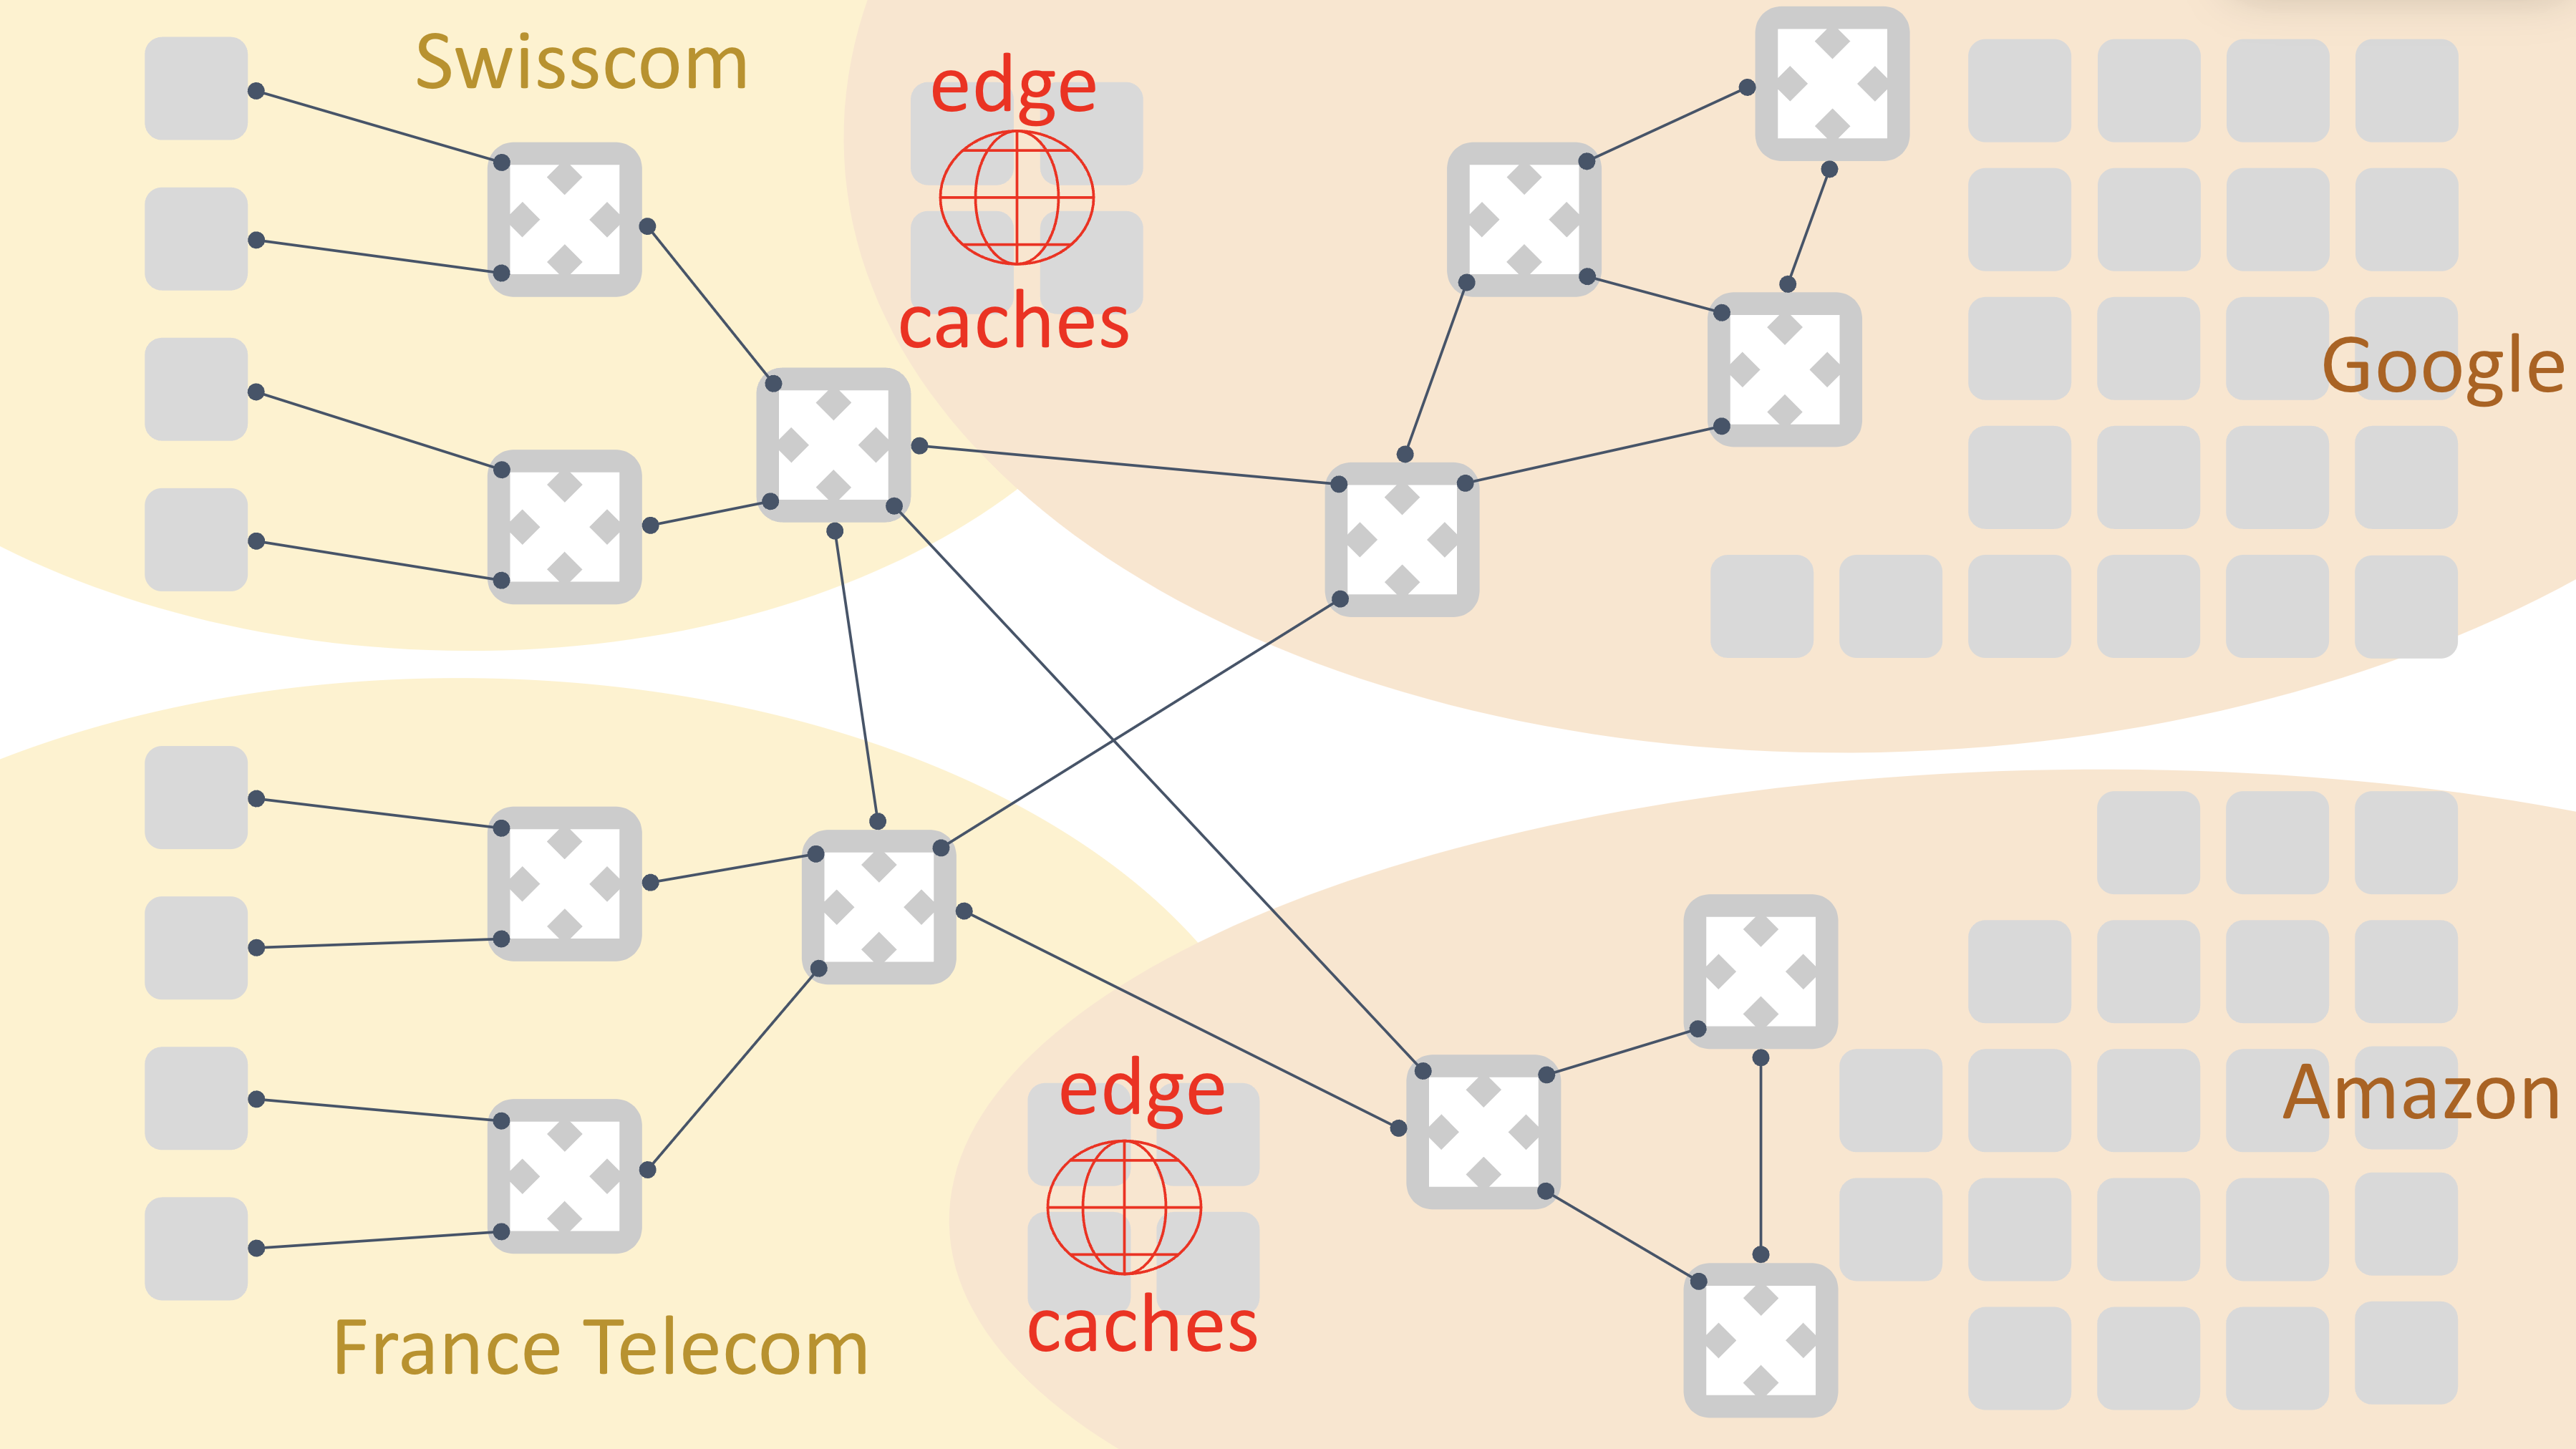
\includegraphics[width=0.65\textwidth]{chapters/L1/images/edge_caches.png}
\end{center}
%%%%%%%%%%%%%%%%%%%%%%%%%%%%%%%%%%%%%%%%%%%%%%%%%%%%%%%%%%%%%%%%%%%%%%
\section{Summary}
In this lecture, we traced the journey of a YouTube video and introduced several fundamental concepts:
\begin{itemize}
  \item \textbf{Programs, Processes, and Threads:} Programs stored on disk become processes (and threads) when executed.
  \item \textbf{Distributed Applications:} Different processes communicate over networks using well-defined communication protocols.
  \item \textbf{Interfaces and Abstractions:} System calls, APIs, and caching abstract the complexity of hardware resources.
  \item \textbf{The Operating System:} Acts as an intermediary between processes and hardware resources.
  \item \textbf{Performance Considerations:} Frequency imbalances between the CPU and memory are mitigated by caching at various levels (CPU cache, file system cache, object caches).
\end{itemize}

\begin{center}
  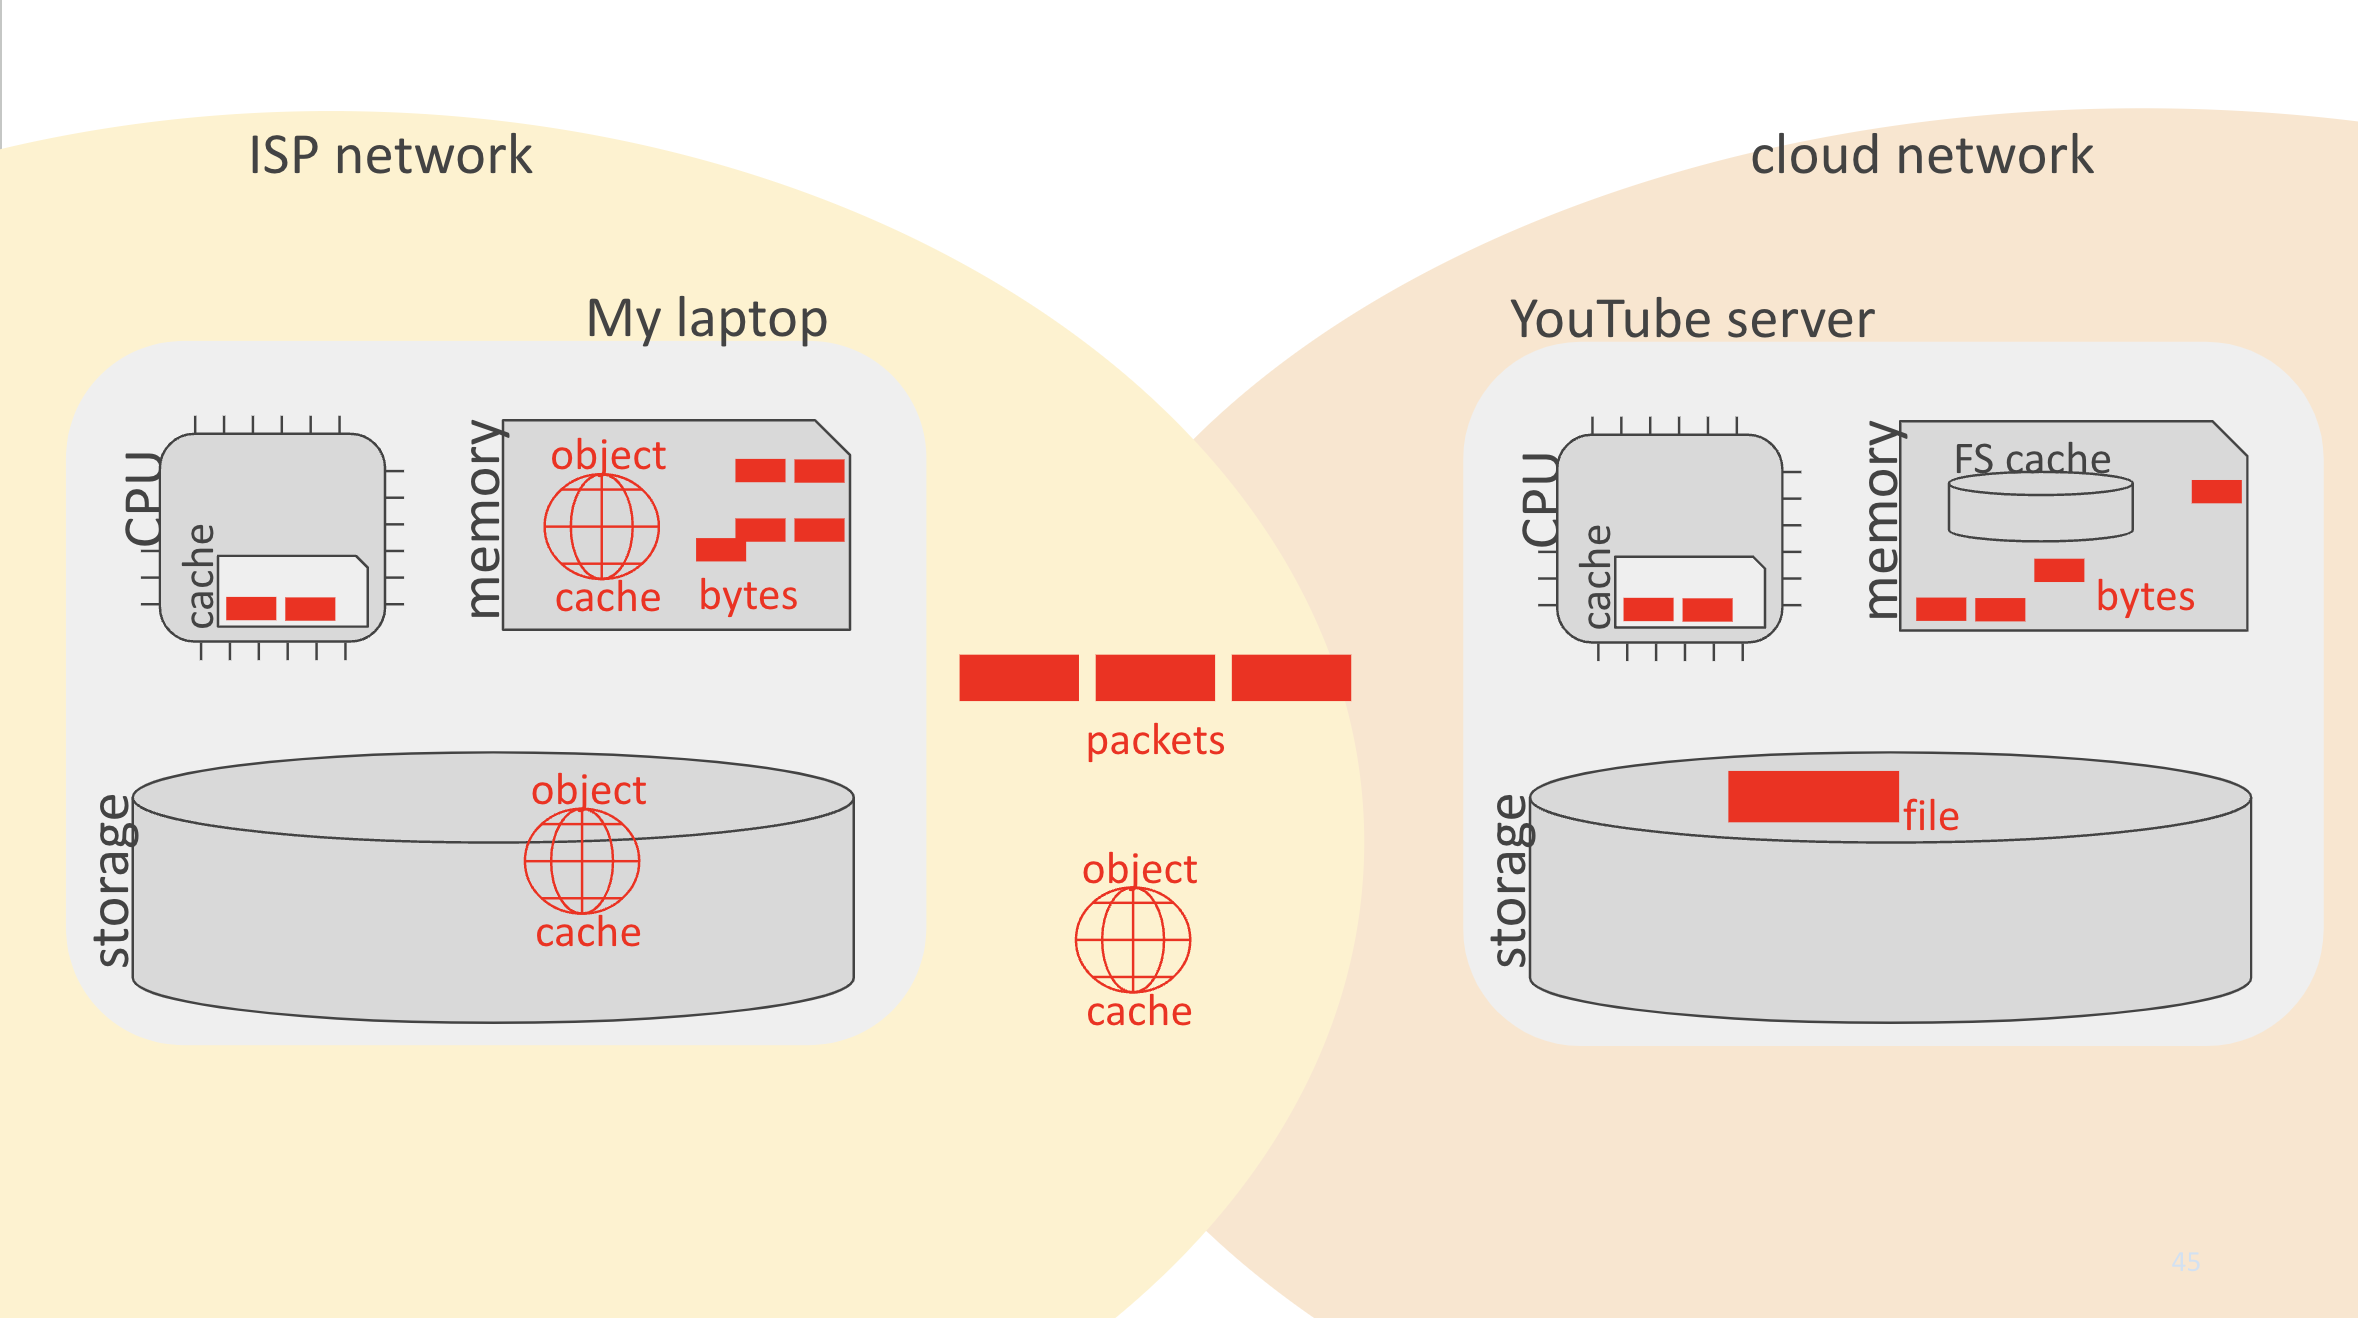
\includegraphics[width=0.65\textwidth]{chapters/L1/images/conclusion_youtube.png}
\end{center}

 

\chapter{L2 - All About Processes}
This chapter provides an overview of the fundamental concepts underlying modern process management and memory organization in computer systems. We discuss multithreading, CPU registers, the role of compilers, and memory organization—including both stack and heap memory—as well as virtualization techniques that allow multiple processes to coexist seamlessly.
\small
\section{Multithreading}
When a program runs, the processor loads it into main memory and creates a thread. In a multithreaded program, there is typically one \emph{manager} thread that delegates work to several \emph{worker} threads. For instance, when computing the sum of a large set of numbers, the workload can be divided into subsets, with each worker thread processing a portion of the data while the manager coordinates the overall computation.

\begin{center}
    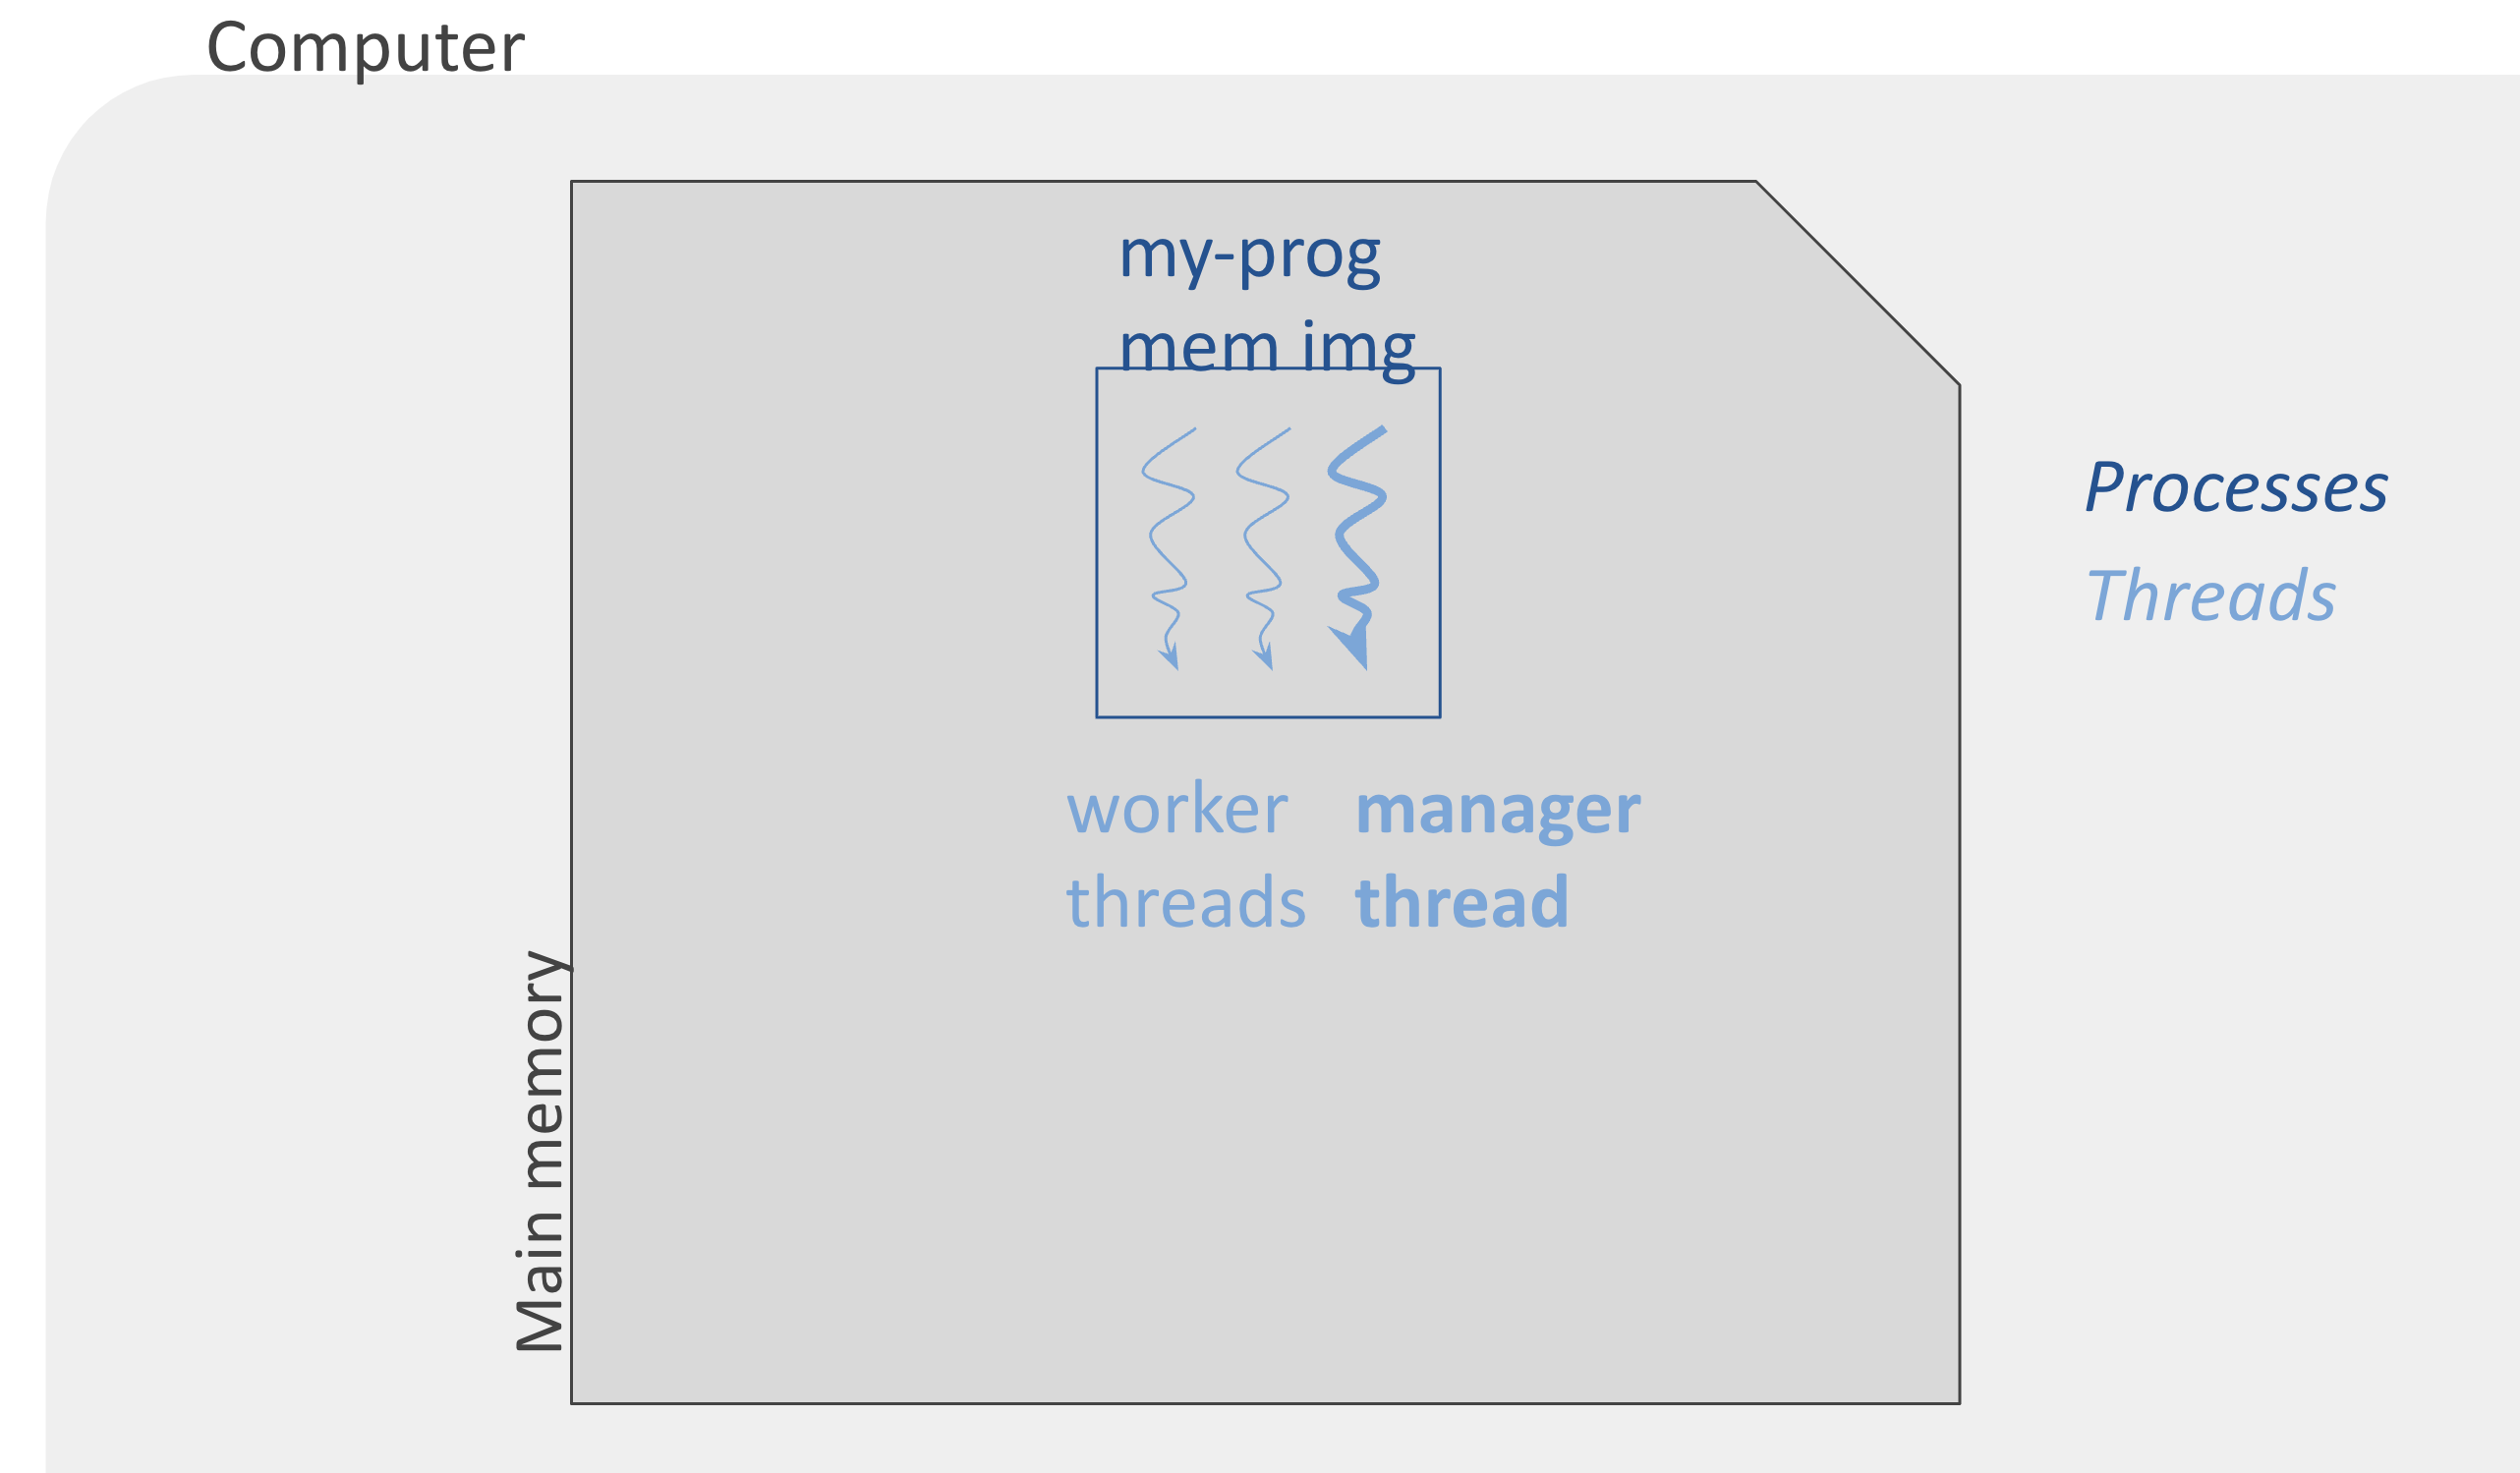
\includegraphics[width=0.55\textwidth]{chapters/L2/images/multi_threads.png}
\end{center}

\section{Registers}
\begin{minipage}{0.45\textwidth}
CPU registers are small storage locations within the processor that hold data and instructions needed during execution. For example, the \texttt{mov} instruction might transfer data from one register (or memory location) to another. Key registers include:
\begin{itemize}
  \item[-] \textbf{Instruction Pointer (IP):} Keeps track of the next instruction to be executed.
  \item[-] \textbf{Stack Pointer (SP):} Points to the current top of the stack in main memory.
\end{itemize}
\end{minipage}
\hfill
\vline
\hfill
\begin{minipage}{0.45\textwidth} 
\begin{center}
    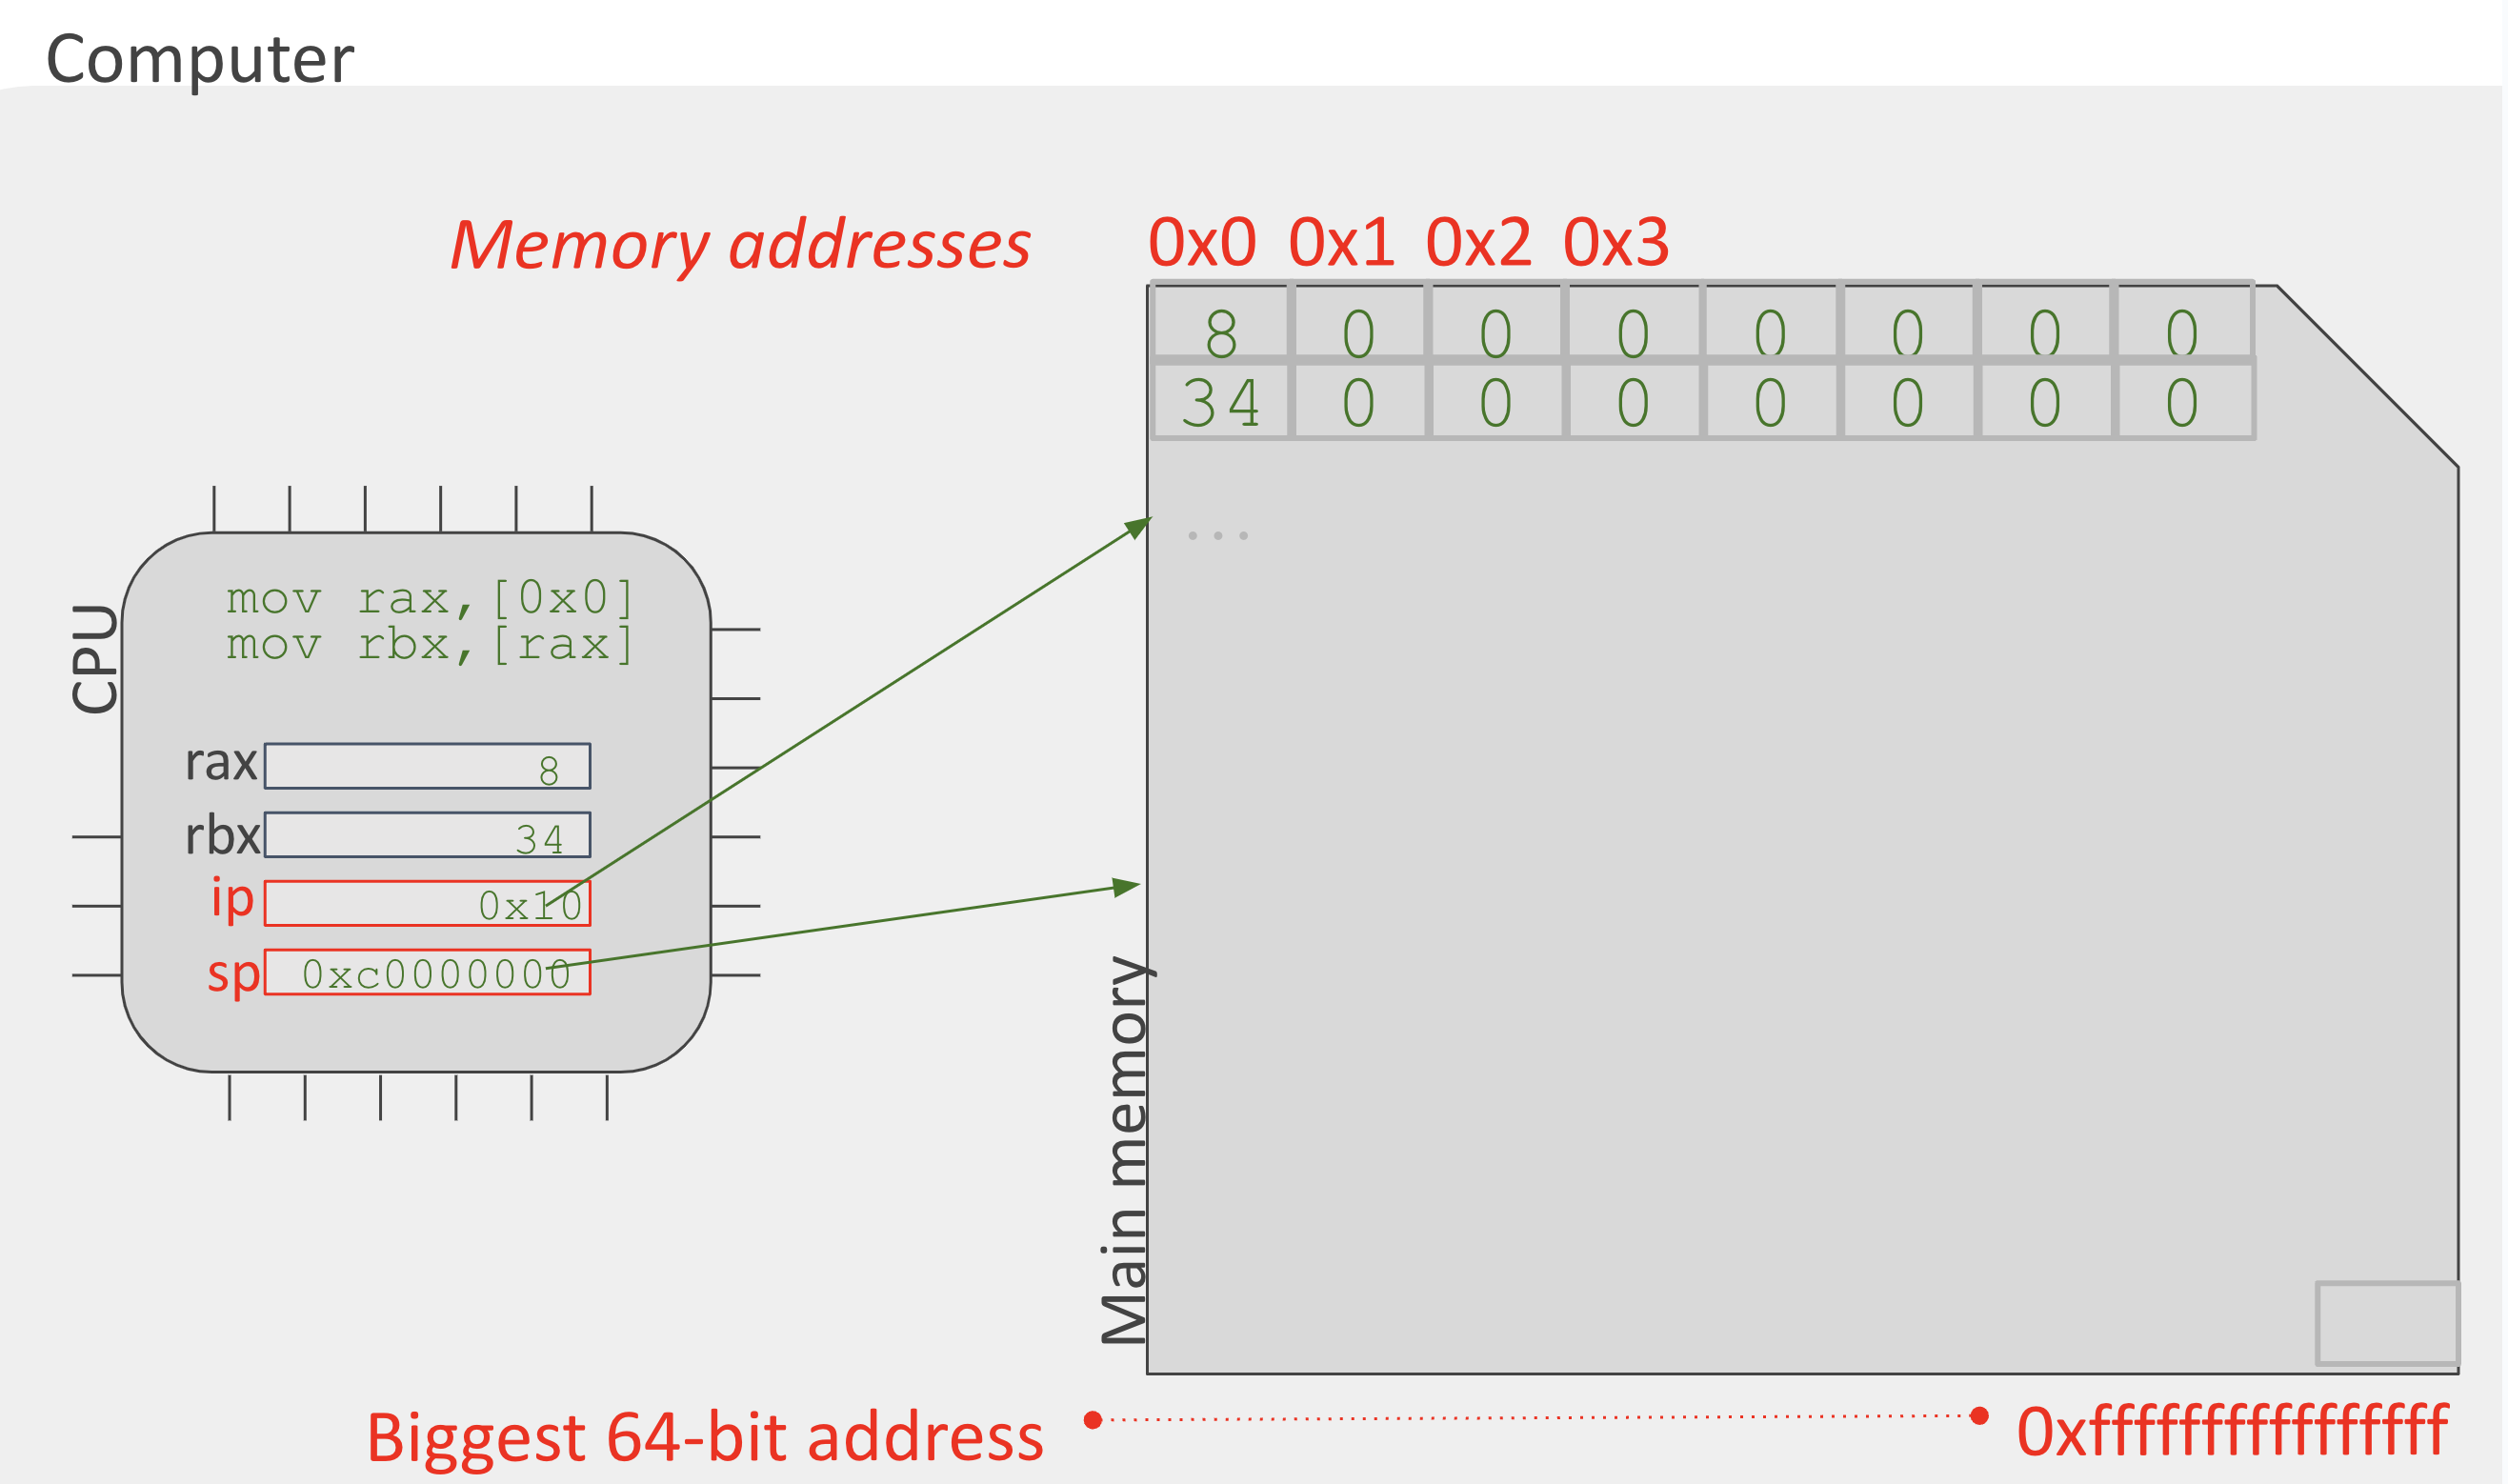
\includegraphics[width=1.1\textwidth]{chapters/L2/images/registers.png}
\end{center}
\end{minipage}
\newpage
\begin{definition}[Compiler]
A compiler translates high-level source code (such as C) into low-level executable code (often Assembly language). This translation involves parsing, optimization, and the generation of machine-specific instructions.
\end{definition}

\section{Memory Organization}
\textit{I'll go a little bit deeper for our fellow syscoms, I also recommend understanding how LIFO works before reading this, if you're too lazy for that, it's basically in the name Last In First Out, means that the last item pushed onto the stack is the first one to be removed, just like stacking plates— you take the top plate first before reaching the ones below. } \\
In modern computer architectures, a process's memory is divided into several distinct segments, each serving a specific role during program execution. Understanding these segments is fundamental for effective programming and debugging. \\[10px]

\begin{definition}[Memory Segments]
A process's memory image is typically divided into the following segments:
\begin{itemize}
    \item \textbf{Text Segment:} Contains the executable code and embedded constants. It is usually marked as read-only to prevent accidental modification.
    \item \textbf{Data Segment:} Stores global and static variables. This segment is often subdivided into:
        \begin{itemize}
            \item \textbf{Initialized Data:} Variables explicitly initialized by the programmer.
            \item \textbf{Uninitialized Data (BSS):} Variables that are declared but not explicitly initialized, and are set to zero by default.
        \end{itemize}
    \item \textbf{Heap Segment:} Used for dynamic memory allocation. Memory here is allocated and deallocated during runtime by the programmer (or automatically via garbage collection in some languages). The heap typically grows upward (from lower to higher memory addresses).
    \item \textbf{Stack:} Manages function calls, local variables, and function parameters. The stack is automatically managed by the CPU, growing downward (from higher to lower memory addresses) as functions are called.
\end{itemize}
\end{definition}

\subsection{The Stack}

The stack is a dedicated region of memory that the CPU uses to manage function calls and local variables. When a function is invoked:
\begin{enumerate}
    \item The CPU executes a \texttt{call} instruction, which pushes the return address onto the stack.
    \item A new \emph{stack frame} is created to store local variables and function-specific data.
    \item Upon function return, the stack frame is removed (or "unwound"), and control returns to the calling function.
\end{enumerate}

\begin{minipage}{0.45\textwidth}
\textbf{Key Characteristics of the Stack:}
\begin{itemize}
    \item \textbf{Automatic Management:} The CPU automatically handles pushing and popping of data.
    \item \textbf{Growth Direction:} Grows downward, from higher to lower memory addresses.
    \item \textbf{Contents:} Stores return addresses, local variables, and sometimes function arguments.
\end{itemize}
\end{minipage}
\hfill
\begin{minipage}{0.45\textwidth}
\begin{center}
    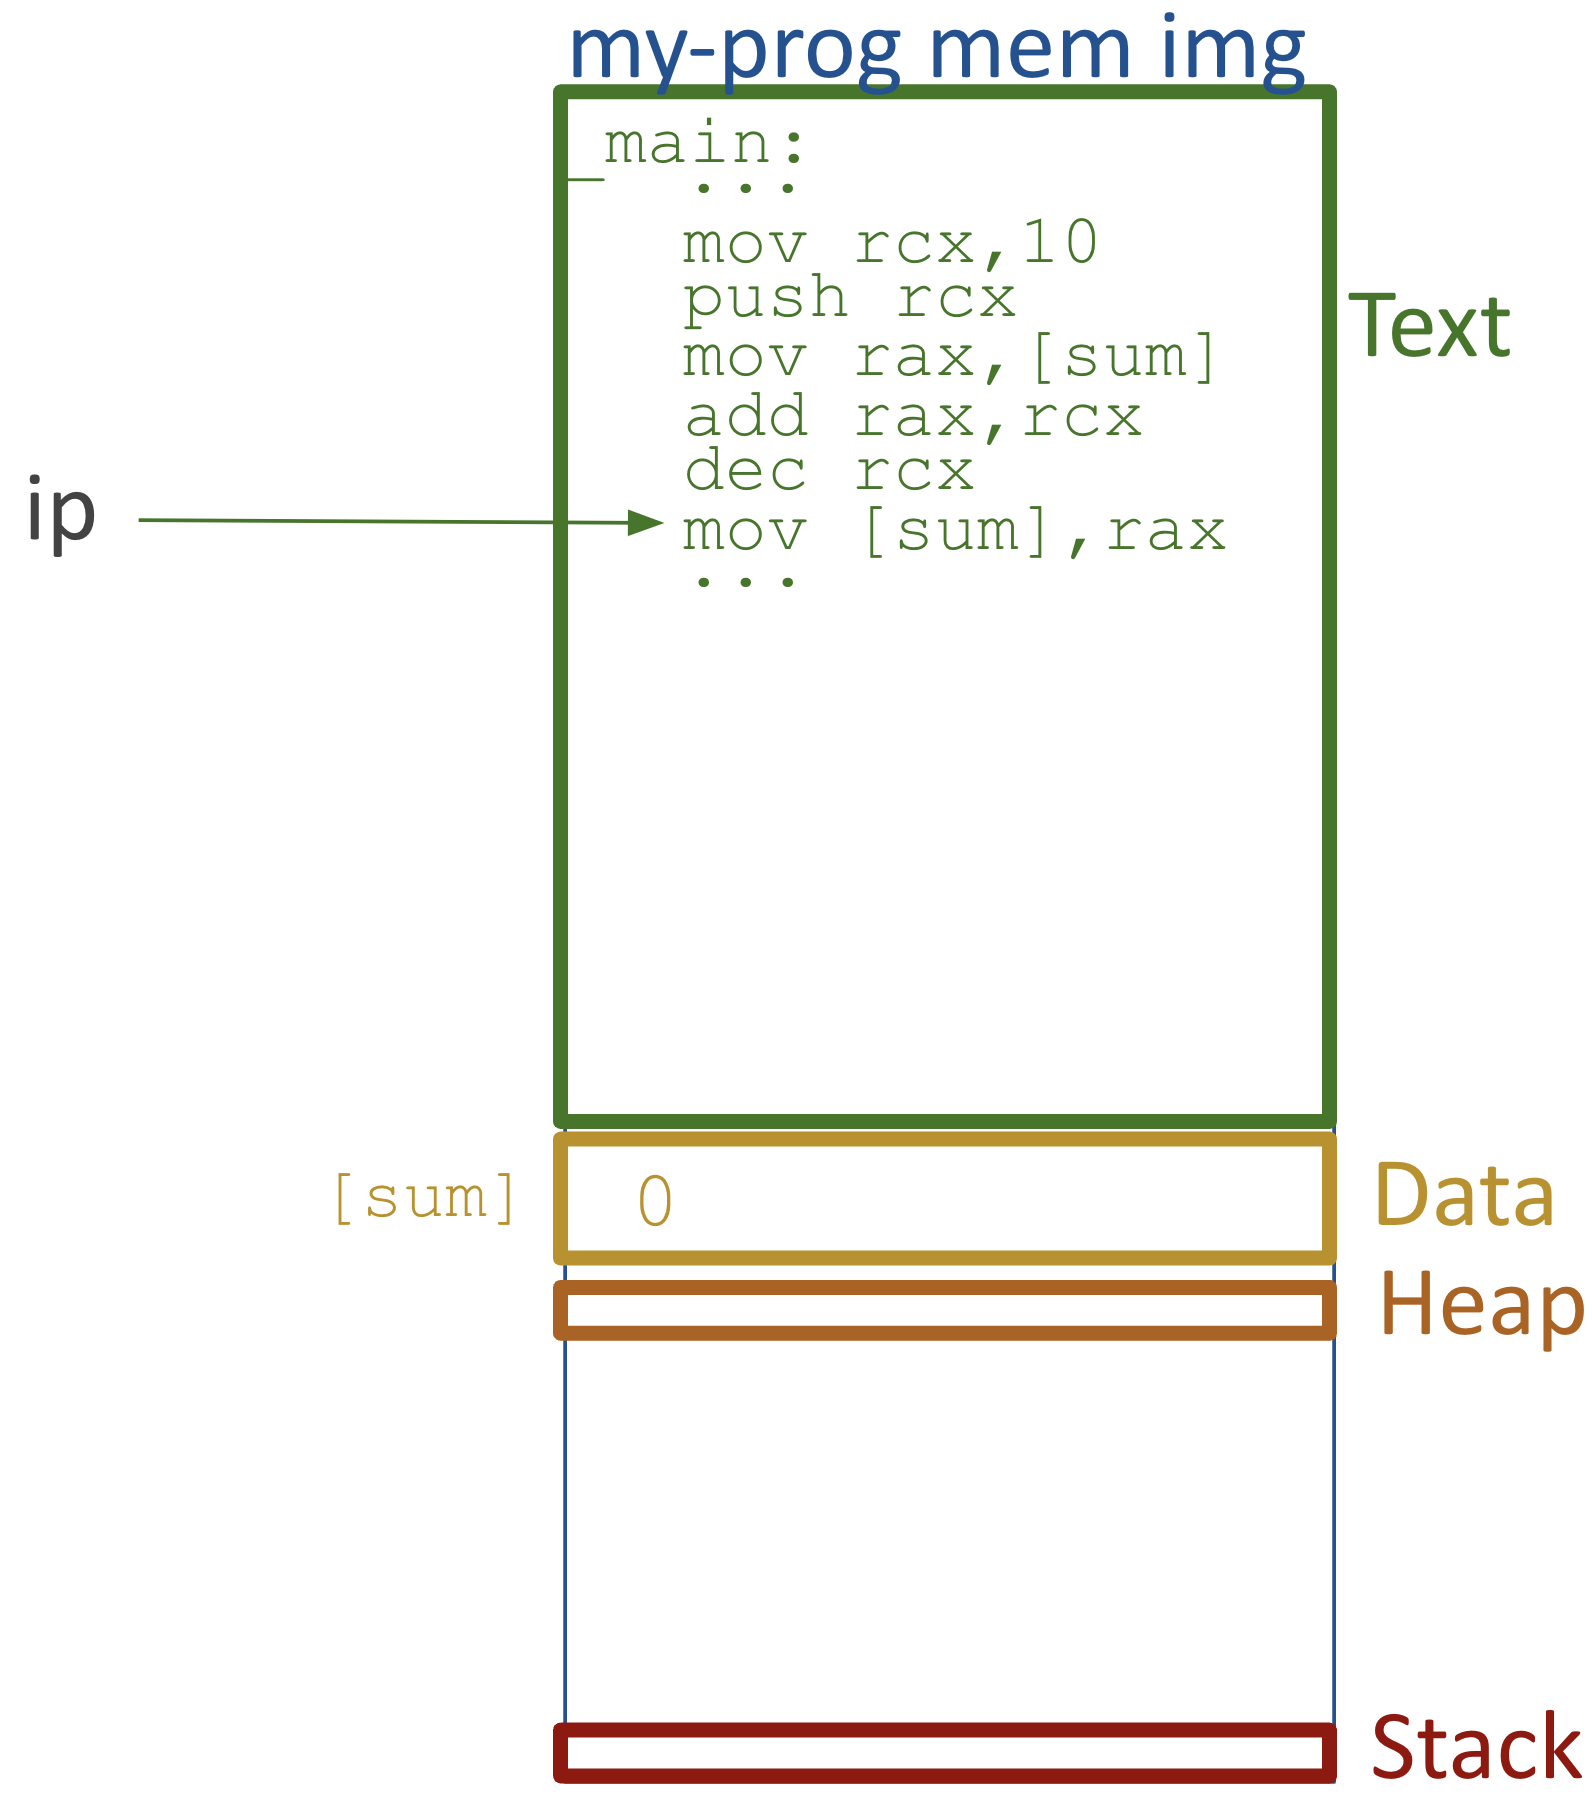
\includegraphics[width=0.75\textwidth]{chapters/L2/images/stack.png}
\end{center}
\end{minipage}

\subsubsection{Stack Frames}
Each function call creates its own \emph{stack frame}, a self-contained section that isolates the function's local data. This segmentation helps maintain the correct scope and lifetime for local variables and ensures that return addresses are preserved. The following diagram illustrates the organization of stack frames during nested function calls:

\begin{center}
    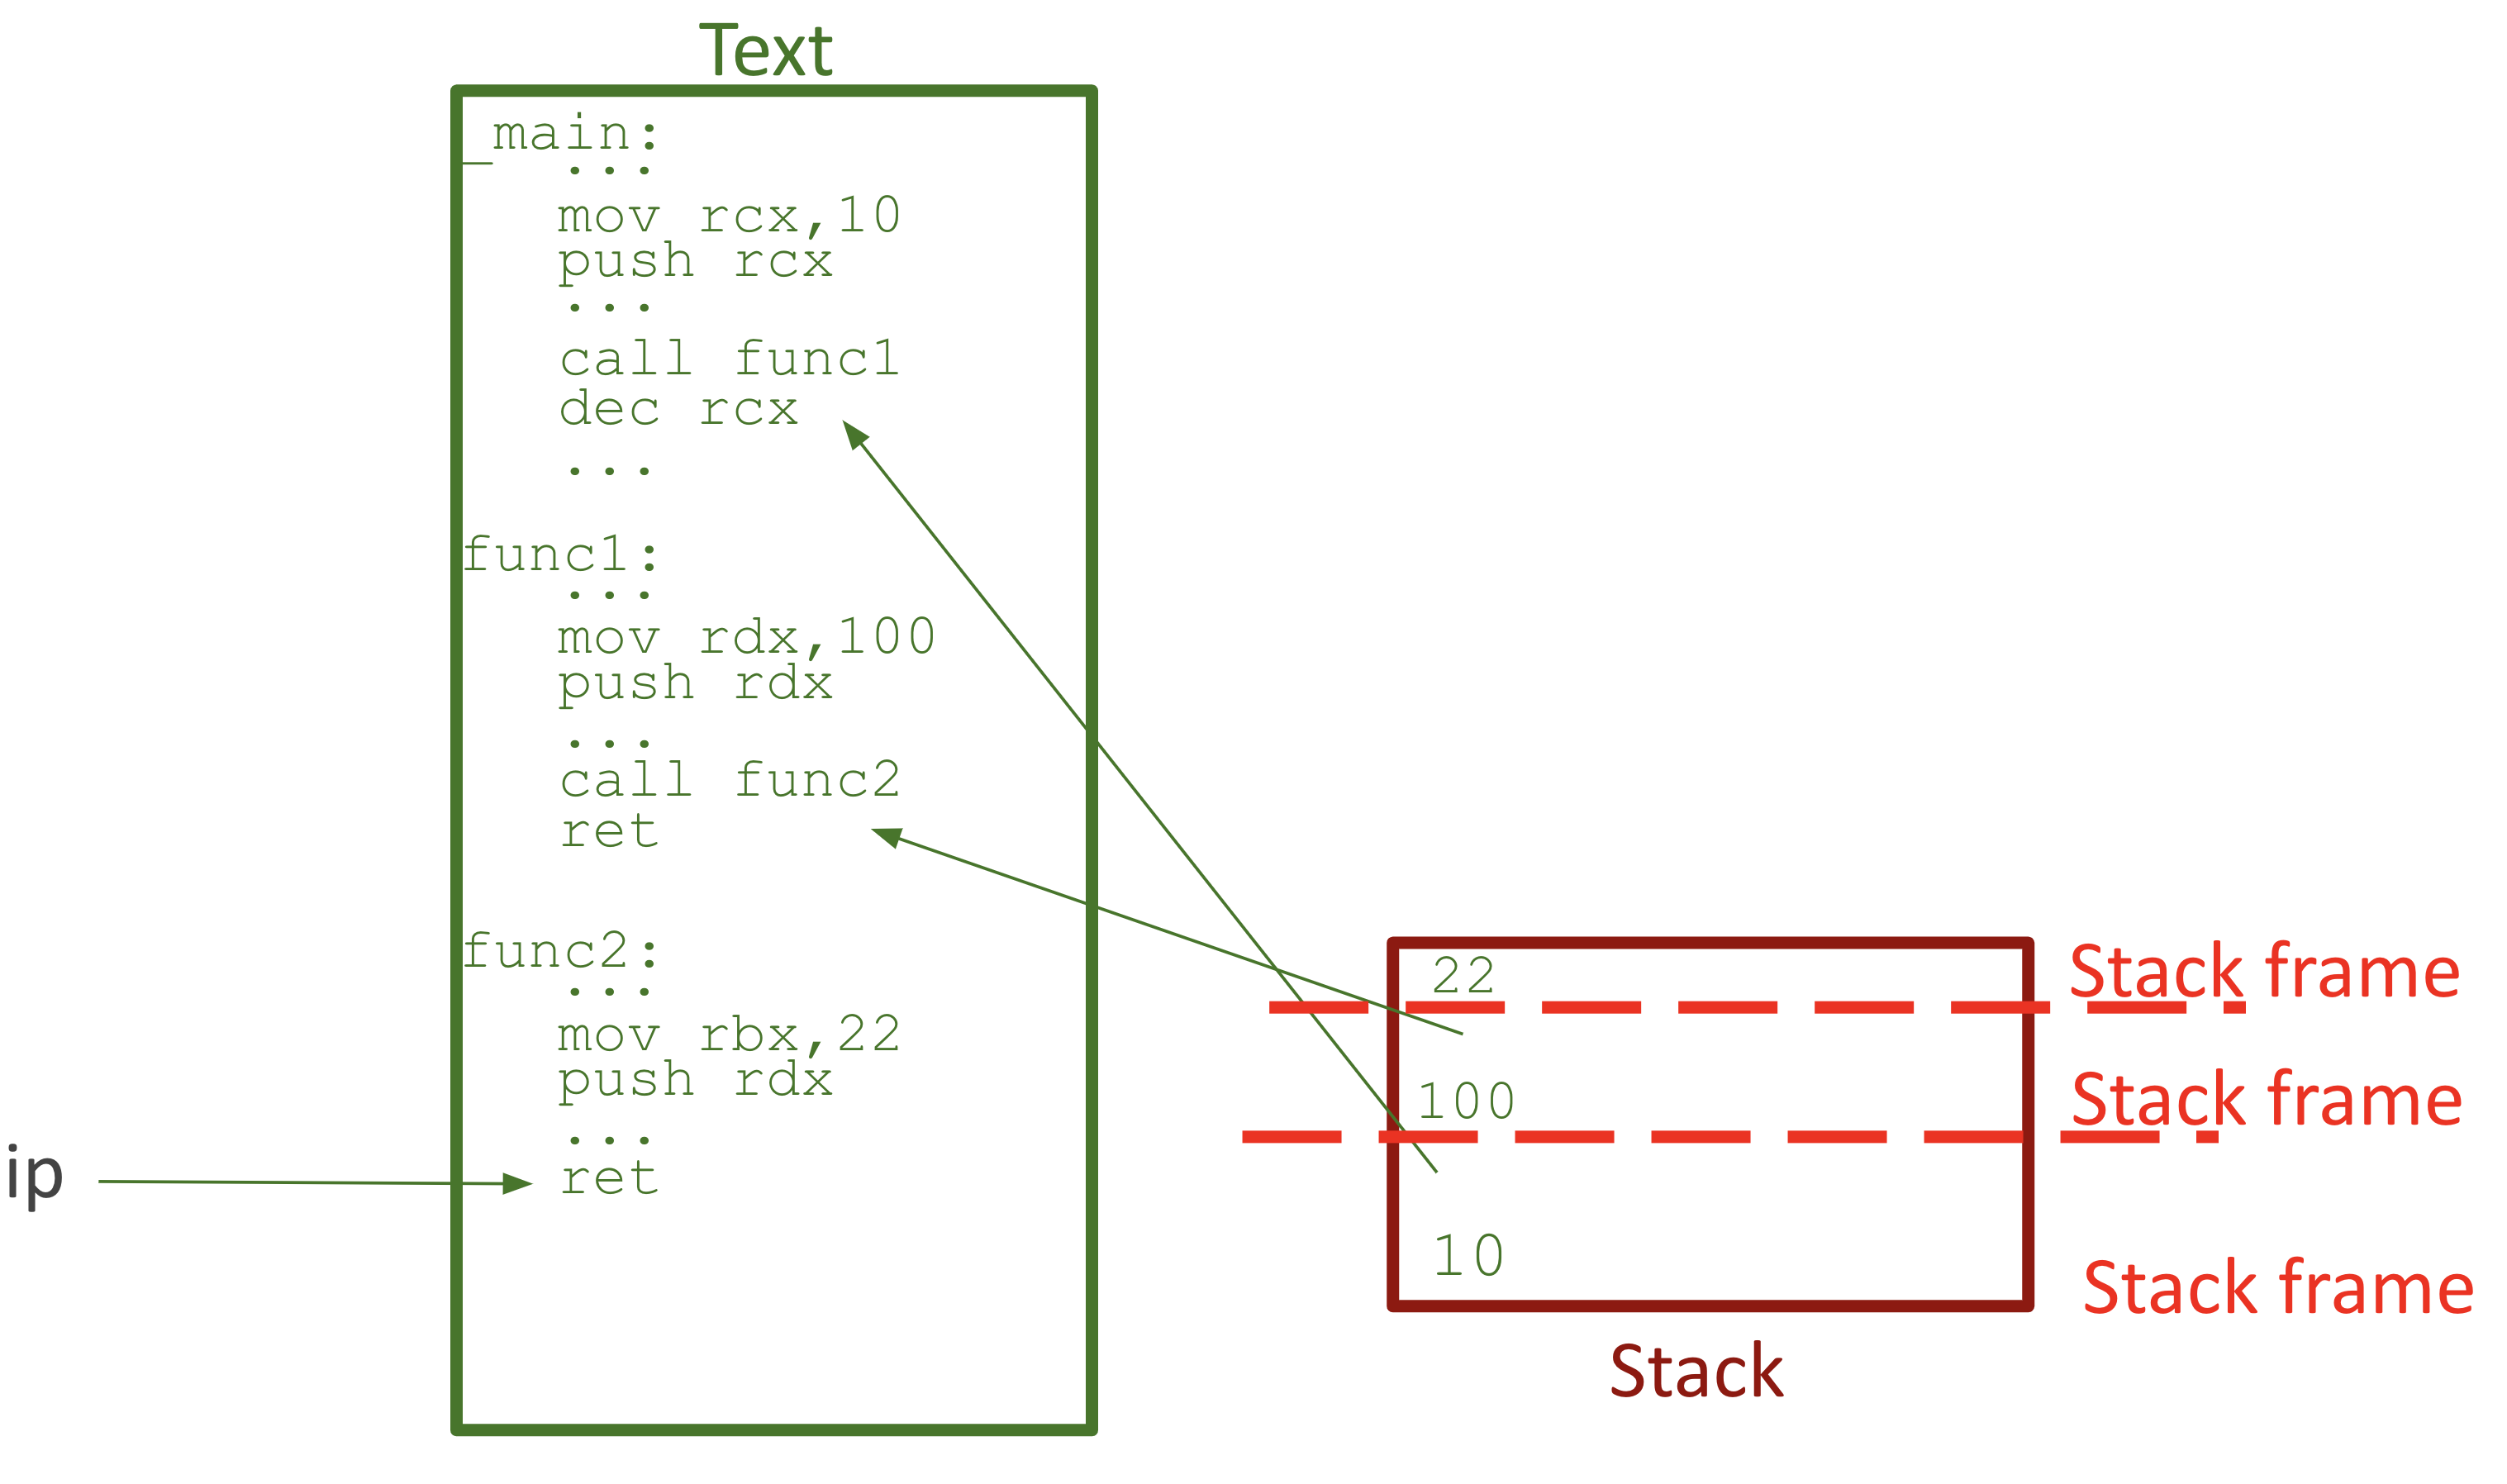
\includegraphics[width=0.65\textwidth]{chapters/L2/images/frames.png}
\end{center}

\subsection{Heap Memory}
The heap is used for dynamic memory allocation, where memory is allocated and deallocated as needed during runtime. Unlike the stack:
\begin{itemize}
  \item[-] \textbf{Manual vs. Automatic Management:} In languages such as C or C++, the programmer is responsible for explicitly allocating (using \texttt{malloc} or \texttt{new}) and deallocating (using \texttt{free} or \texttt{delete}) heap memory. In contrast, some modern languages employ automatic garbage collection.
  \item[-] \textbf{Growth Direction:} The heap typically grows upward, from lower to higher memory addresses.
  \item[-] \textbf{Lifetime:} Data allocated on the heap persists beyond the scope of the function that created it, until it is explicitly freed or garbage collected.
\end{itemize}

\subsection{Data and Text Segments}

\textbf{Text Segment:}  
This segment contains the program's executable code and constant values. Its read-only nature helps prevent inadvertent modifications during execution.
\vspace{0.5em}
\textbf{Data Segment:}  
This segment holds global and static variables. It is divided into:
\begin{itemize}
  \item[-] \textbf{Initialized Data:} Variables that have been assigned an initial value at compile time.
  \item[-] \textbf{Uninitialized Data (BSS):} Variables that are declared but not explicitly initialized; these are automatically set to zero at program startup.
\end{itemize}

\begin{definition}[CPU Registers]
Two registers are critical for process execution:
\begin{itemize}
  \item[-] \textbf{Instruction Pointer (IP):} Points to the next instruction in the text segment.
  \item[-] \textbf{Stack Pointer (SP):} Points to the top of the stack.
\end{itemize}
\end{definition}

\begin{definition}[Process and Thread Identifiers]
\leavevmode\\ % Ensures LaTeX enters vertical mode before inserting a newline
A process is considered to be \emph{running} if at least one of its threads is executing; otherwise, it is not running.
\begin{itemize}
  \item[-] \textbf{Process ID (PID):} A unique identifier assigned to each process.
  \item[-] \textbf{Thread ID (TID):} A unique identifier for each thread, which may be unique within a process or across the entire system, depending on the operating system.
\end{itemize}
\end{definition}

\begin{definition}[Resource Sharing]
Processes and threads share system resources such as CPU and memory. Each thread is given the illusion of having exclusive access to the CPU, and each process appears to have dedicated memory, even though these resources are actually shared.
\end{definition}
\vspace{10px}

\begin{definition}[CPU Sharing]
The CPU is time-shared among multiple threads. This virtualization is achieved through context switching, where the CPU rapidly switches between threads, giving each one the impression of exclusive use of the processor.
\end{definition}

\subsubsection{Example: Two Programs Running on a Single Core}
\begin{example}
Consider two programs running on a single-core processor. Each program is assigned a CPU context, which includes register values such as \texttt{rax}, \texttt{rbx}, the stack pointer (SP), and the instruction pointer (IP). When switching between programs, the CPU saves the current context to memory and loads the context of the next program, allowing the programs to resume correctly.
\end{example}

\begin{center}
    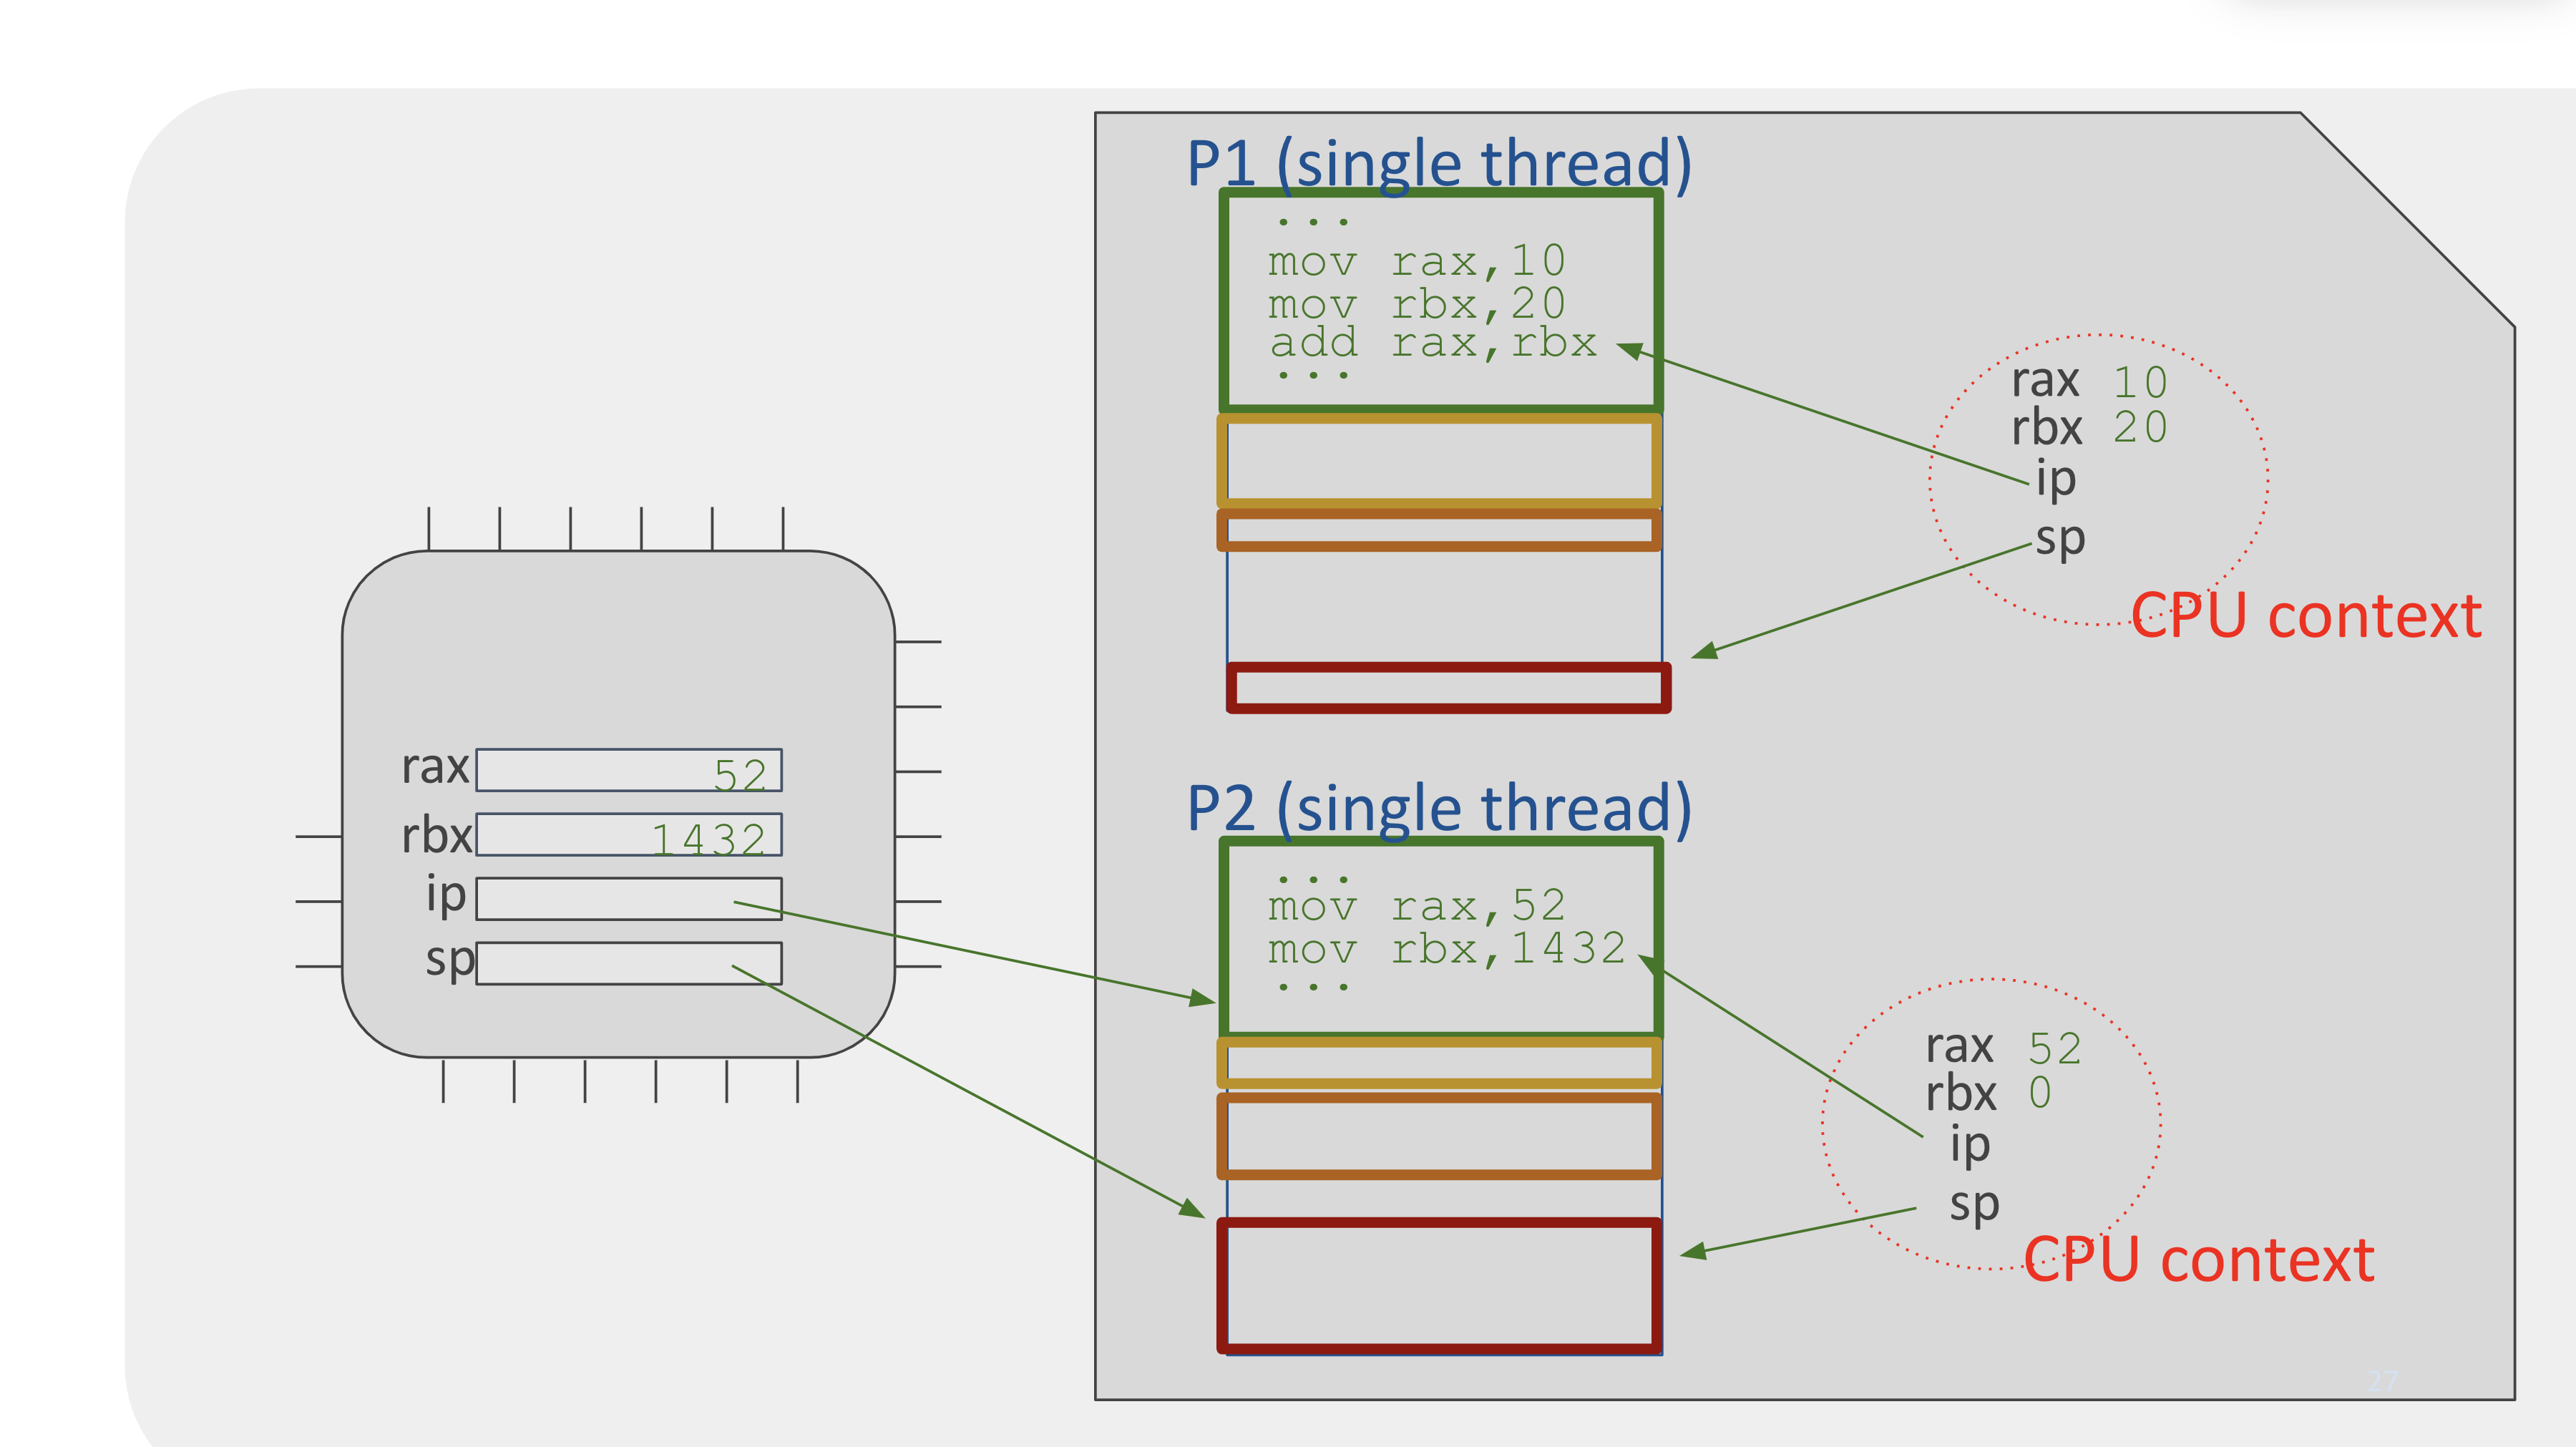
\includegraphics[width=0.8\textwidth]{chapters/L2/images/cpu_context.png}
\end{center}

\begin{definition}[Thread's CPU Context]
A thread's CPU context comprises the values of all CPU registers at the moment it was last executing. In a single-threaded process, this context represents the entire process state.
\end{definition}

\begin{definition}[Context Switching]
Context switching is the process by which the CPU switches from executing one thread to another. It involves:
\begin{enumerate}
    \item Saving the current thread's CPU context to memory.
    \item Restoring the CPU context of the thread to be executed next.
    \item[] Each thread has the illusion that it's occupying the CPU \textbf{alone}.
\end{enumerate}
This mechanism enables CPU virtualization but introduces performance overhead due to additional memory accesses.
\end{definition}
\vspace{10px}
\begin{definition}[Process]
A process is defined by:
\begin{itemize}
    \item A unique Process ID (PID).
    \item A memory image that includes the text, data, heap, and stack segments.
    \item The CPU contexts of each thread within the process.
    \item Associated resources such as file descriptors.
\end{itemize}
\end{definition}
\textit{Remark: If two threads belong to the same process, does each have its own CPU context, or do they share one? The answer is that each thread should be able to continue its execution independently.}
\vspace{10px}
\begin{definition}[Memory Sharing]
Memory in a system is space-shared among processes; however, virtualization ensures that each process operates within its own isolated address space. This is achieved through virtual-to-physical address translation.
\end{definition}
\vspace{10px}
\begin{definition}[Virtual and Physical Addresses]
Virtual addresses allow processes to operate as if they have exclusive access to memory. For example, two processes might both use the virtual address \texttt{0x400000}; however, these addresses map to different physical addresses:
\begin{itemize}
  \item[-] Process \( P_1 \): Virtual \texttt{0x400000} \(\rightarrow\) Physical \texttt{0x1234AFF8}
  \item[-] Process \( P_2 \): Virtual \texttt{0x400000} \(\rightarrow\) Physical \texttt{0xABCD5678}
\end{itemize}
\end{definition}
\vspace{10px}
\begin{definition}[Virtual Address Space]
Each process is allocated its own virtual address space, which is shared among all its threads. This abstraction allows developers to ignore the complexities of physical memory allocation.
\end{definition}
\vspace{10px}
\begin{definition}[Address Translation]
Address translation is the process by which a virtual memory address is converted into a physical memory address. While essential for memory virtualization, this translation incurs a performance cost.
\end{definition}

\subsection{Stack Smashing}
Stack smashing is a type of buffer overflow vulnerability where an attacker deliberately overwrites parts of the memory on the call stack. This typically happens when a program writes more data into a fixed-size buffer than it can accommodate, thereby corrupting adjacent memory areas such as the function's return address.

\paragraph{How It Works:}
When a function is called, a stack frame is created that contains local variables, return addresses, and other control data. If a buffer does not have proper bounds checking, an input exceeding the buffer's capacity can overflow into these critical areas. For example:
\begin{enumerate}
    \item A fixed-size buffer is allocated on the stack.
    \item Excess input data overwrites memory beyond the buffer.
    \item The return address (or other control data) is corrupted.
    \item On function return, control is transferred to an address chosen by the attacker, potentially executing malicious code.
\end{enumerate}
\subsection{Summary: CPU and Memory Virtualization}
\begin{itemize}
    \item \textbf{CPU Virtualization:} Threads time-share the CPU through context switching, which gives each thread the illusion of exclusive CPU access.
    \item \textbf{Memory Virtualization:} Processes space-share memory via virtual-to-physical address translation, ensuring that each process operates in its own isolated address space.
\end{itemize}

\subsection{Conclusion}
Modern operating systems are designed to enable multiple programs to share CPU and memory resources seamlessly. Through context switching and address translation, both the CPU and memory are effectively virtualized. This abstraction simplifies development, as compilers and developers can design programs without needing to manage these low-level resource-sharing details directly.


 
\chapter{L3 - Sharing the CPU}

This chapter introduces the mechanisms by which an operating system (OS) manages access to the CPU, ensuring both security and fairness among processes. We discuss CPU privilege levels, the limited direct execution model, and the role of system calls (syscalls) in process management.
\vfill
\section{The OS as a Special Program}

The operating system (OS) is a fundamental software layer that manages hardware resources and provides essential services for user applications. Unlike typical applications, the OS operates at different privilege levels and ensures secure and efficient execution of processes and threads.
\subsection{Limited Direct Execution}
\textbf{Professor Analogy cont. -} The children have direct access to the TV but are restricted by Kids Mode. \\
Limited direct execution is a method that allows a thread to run directly on the CPU while enforcing certain restrictions:
\begin{itemize}
  \item[-] \emph{Direct Execution:} The CPU executes the thread's instructions without any intermediate emulation.
  \item[-] \emph{Limited:} The thread cannot perform operations that require high privileges; instead, it must request system assistance via syscalls.
\end{itemize}
The CPU runs in Limited Direct Execution. Let's see how it's limited 
\newpage
\subsection{CPU Privilege Levels and Execution Modes}
\textbf{Professor Analogy -} Imagine you have children who want to watch TV. You can either keep the remote with you and ask them to call you whenever they need to change the channel, or you can enable Kids Mode on the TV, allowing them limited access without needing to ask for permission each time. \\[3px]
\textit{Personal Remark - Kernal code \emph{always} run in High Privilege mode, and because of this we say that the OS \emph{may} run in High Privilege mode (kernel is inside of the os), do not confuse both !}\\[3px]
The OS shares the CPU and main memory with normal user processes and threads. However, its execution mode differs based on its role at any given time:

\begin{itemize}
  \item[-] When the OS executes, the CPU \textit{may} be in \textbf{high privilege mode} (often called kernel mode), allowing it unrestricted access to all system resources.
\item[-] When a normal process or thread executes, the CPU is in \textbf{low privilege mode} (user mode), restricting access to critical system resources.
\end{itemize}

\begin{center}
  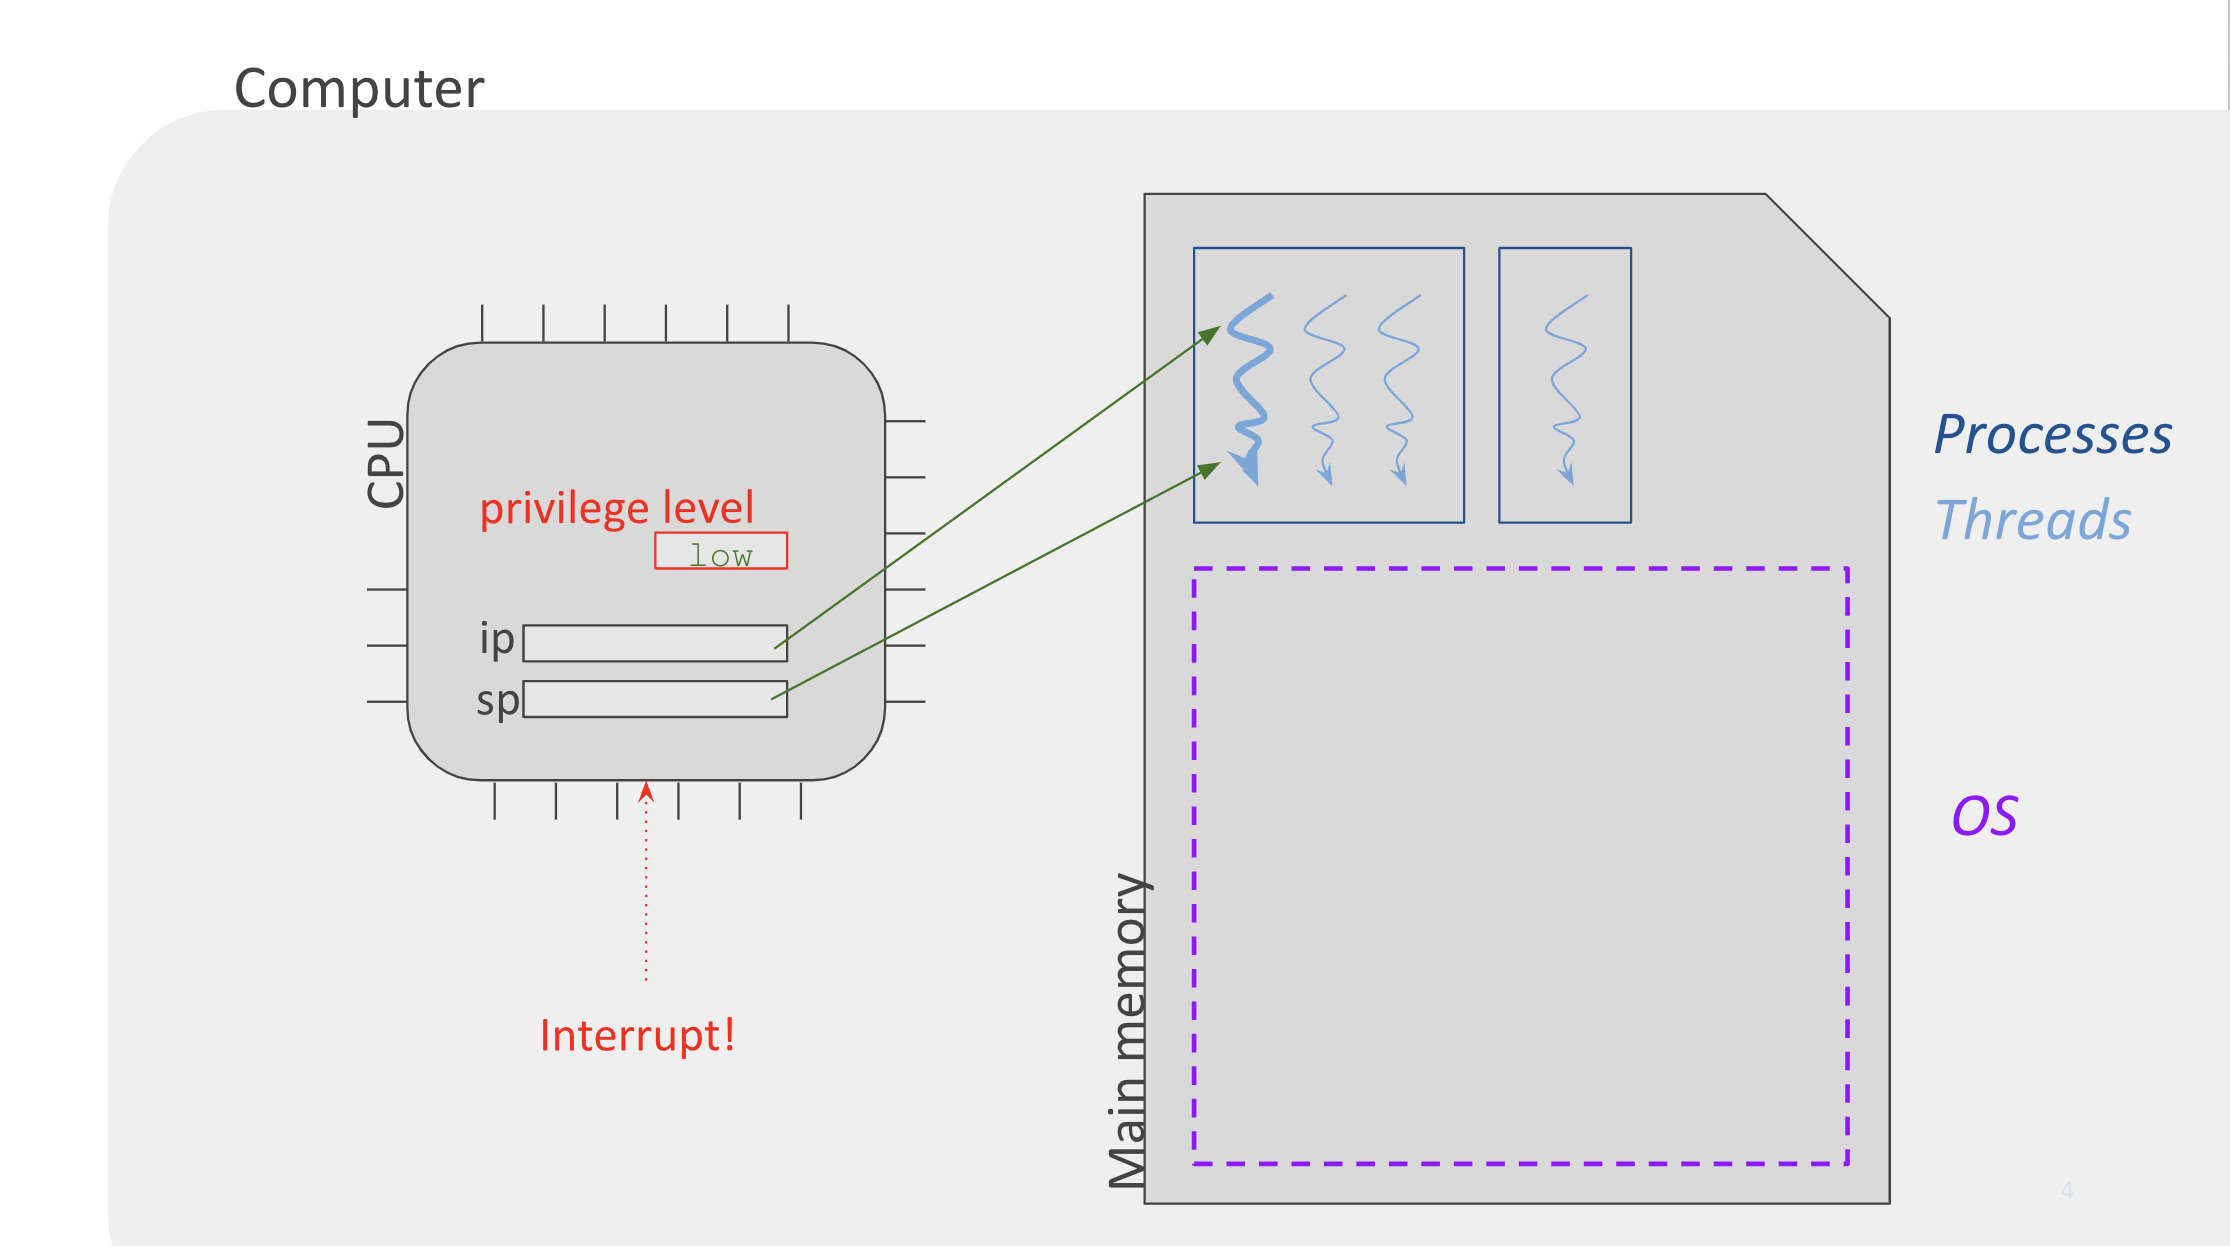
\includegraphics[width=0.8\textwidth]{chapters/L3/images/priviledge.png}
\end{center}

This privilege system exists primarily for security reasons, enforcing the \textbf{principle of least privilege}, where each process has only the necessary access rights required to perform its task. 

\subsection{The Kernel: Core Component of the OS}

A key component of the OS is the \textbf{kernel}, responsible for:

\begin{itemize}
  \item[-] Creating and managing processes and threads.
  \item[-] Allocating system resources (CPU time, memory, I/O devices, etc.).
  \item[-] Ensuring that each process has a designated portion of memory, including stack, data, and text segments.
  \item[-] Enforcing security and isolation between processes.
\end{itemize}

The kernel always runs in \textbf{high privilege mode} (kernel mode), which is why this mode is sometimes referred to as \textit{kernel mode}. 

\subsection{Process Management and Context Switching}

The OS does not execute continuously but rather runs only when necessary. It performs essential tasks, prepares the environment for the next process, and then switches out, allowing user processes to execute.

\begin{itemize}
  \item[-] The OS uses \textbf{context switching} to transition between processes efficiently, preserving the state of the current process before switching to another.
  \item[-] By switching between kernel mode and user mode, the OS ensures that user applications run securely and do not directly manipulate hardware resources.
\end{itemize}

\subsection*{The Loader: Setting Up Process Memory}

Another critical component of the OS is the \textbf{loader}, which is responsible for preparing a program for execution: \\
\begin{minipage}{0.45\textwidth}
\begin{itemize}
    \item[-] The loader completes the setup of the process's memory image.
    \item[-] It copies the command-line arguments used to launch the program (e.g., \texttt{ls -a}, where \texttt{-a} is an argument).
    \item[-] These arguments are stored in the \textbf{stack} of the main thread of the new process to ensure accessibility.
\end{itemize}
\end{minipage} \hfill \vline \hfill 
\begin{minipage}{0.45\textwidth}
If these arguments were stored in the loader's stack instead, the process would not be able to access them after execution begins.
\begin{center}
    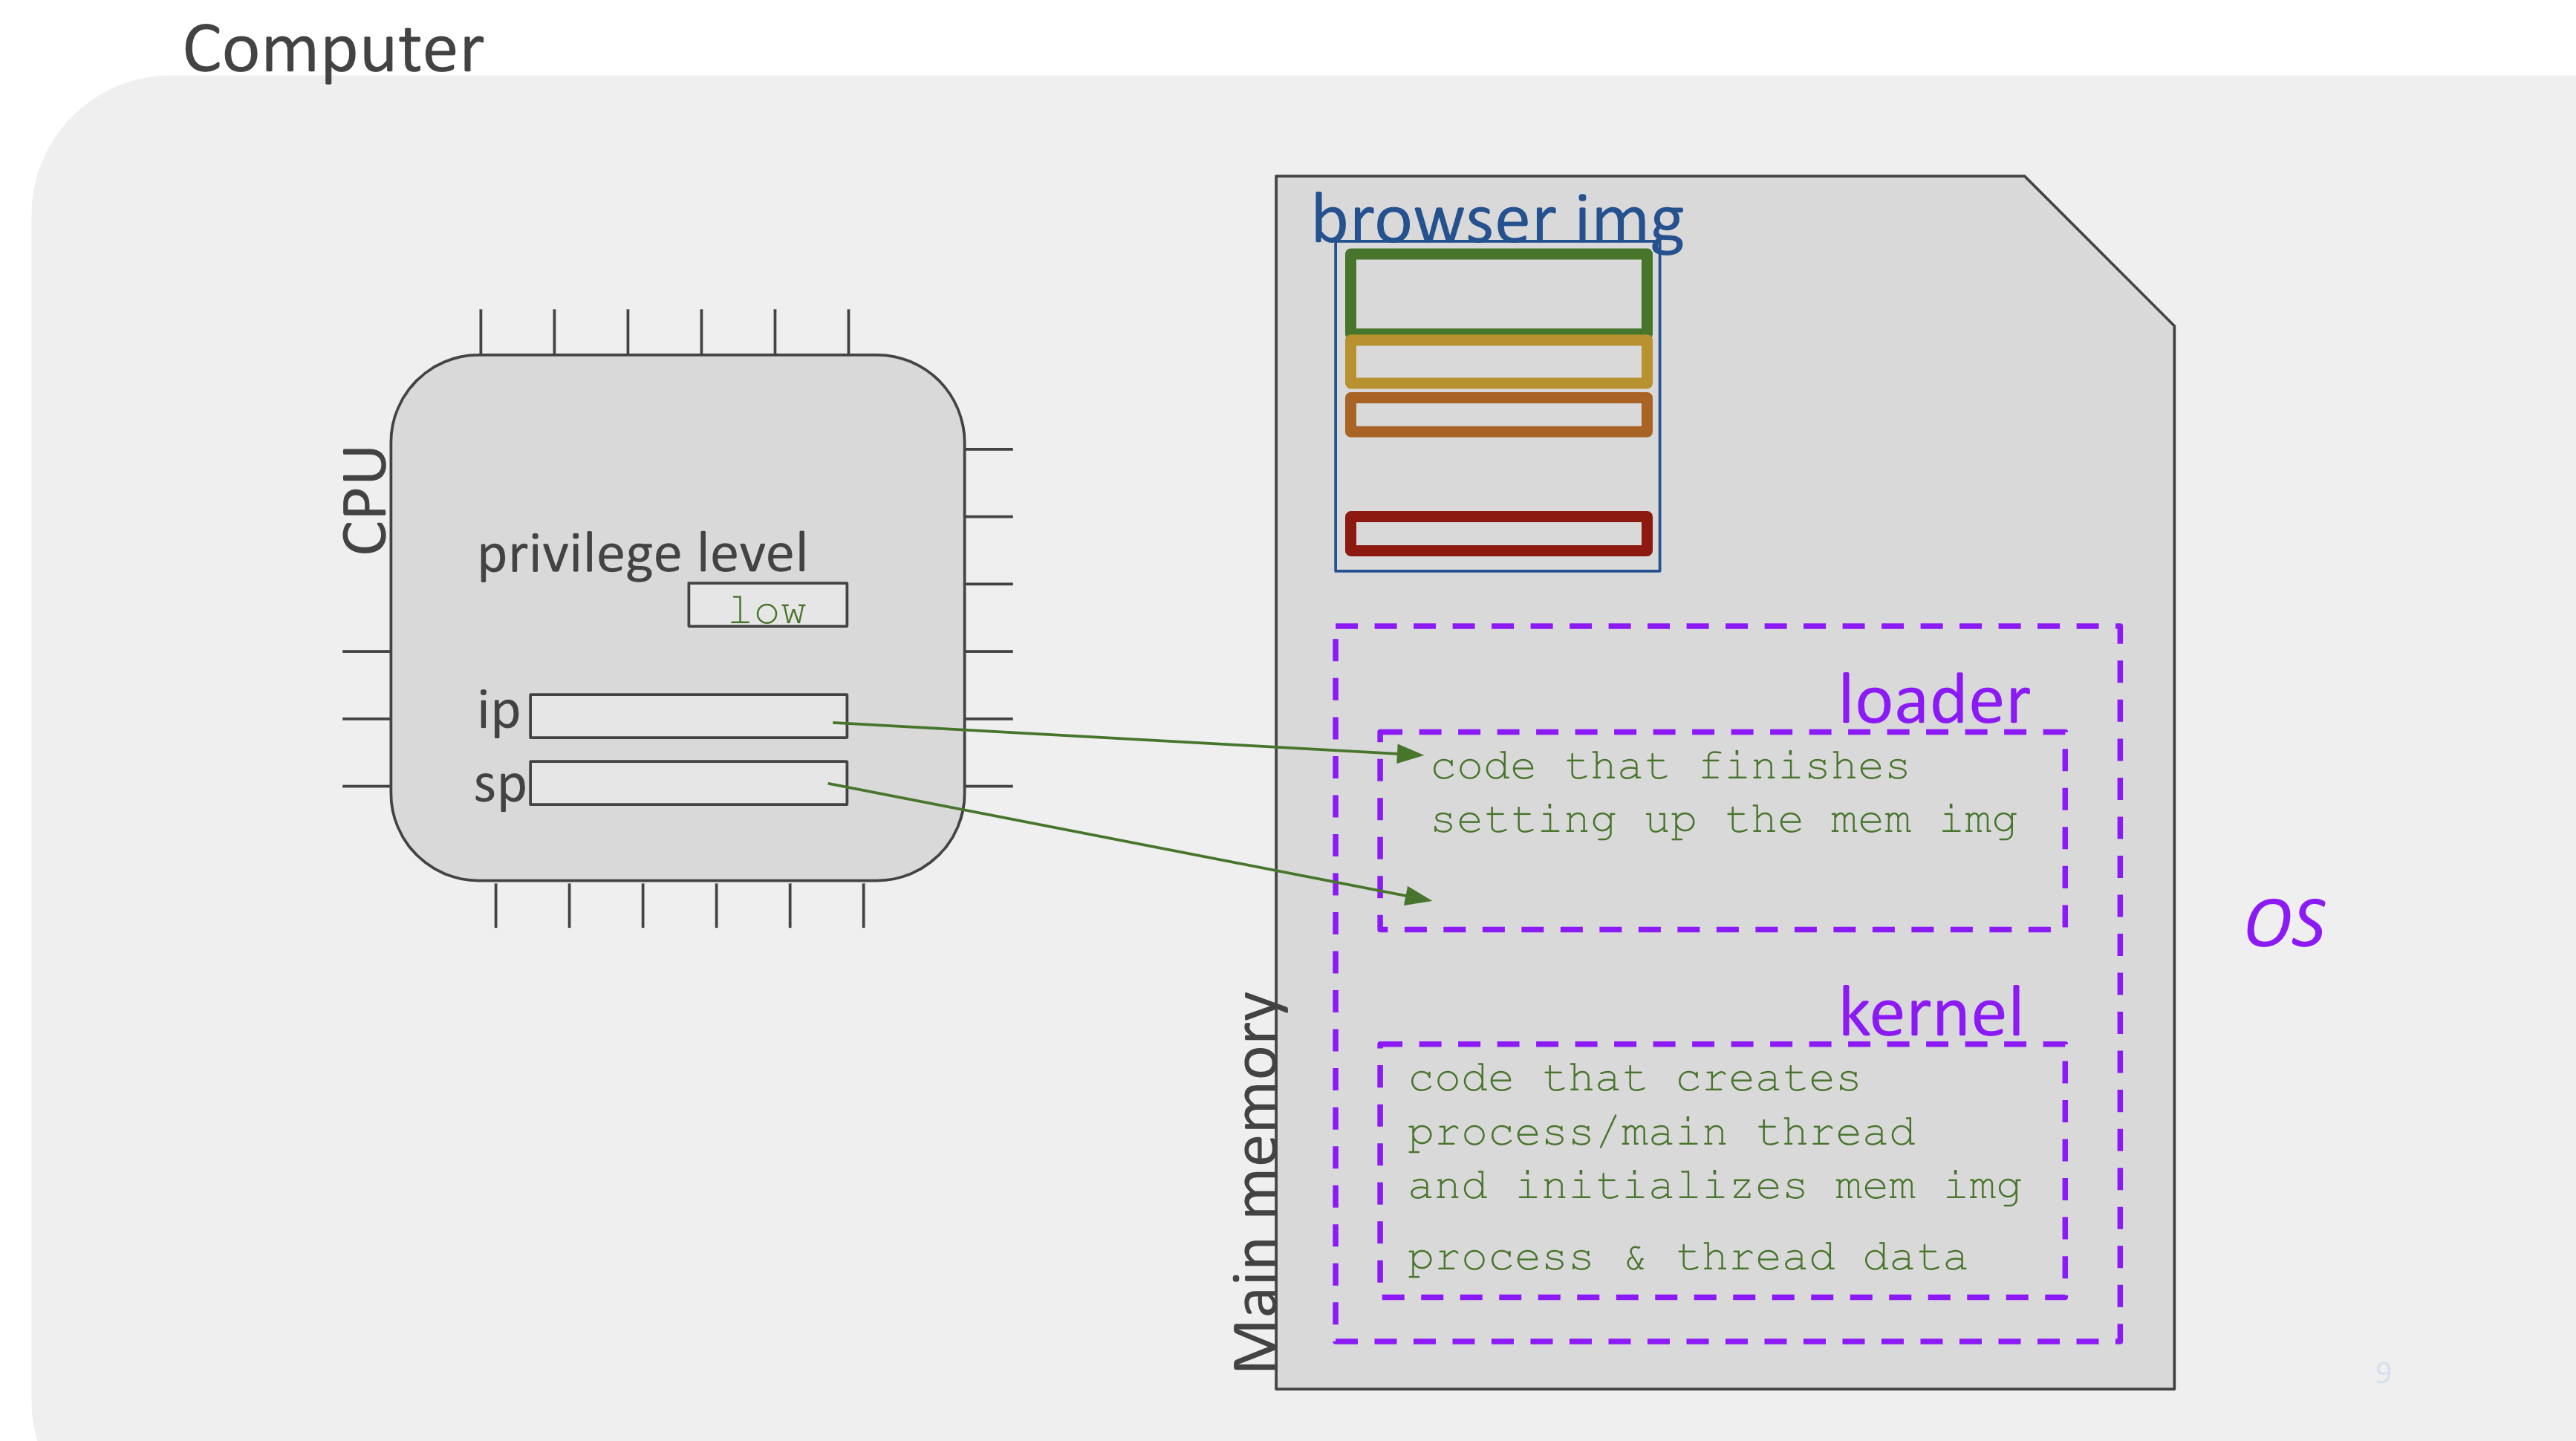
\includegraphics[width=1.1\textwidth]{chapters/L3/images/kernel.png}
\end{center}
\end{minipage} \\[10px]

This layered privilege model ensures a secure and efficient execution environment, maintaining stability and protection across all processes within the system.
\subsection{Syscalls}
\textit{Personal Remark - Syscalls are NOT needed when executing OS code, they only allow to cross the priviledged barrier when running a unpriviledged code.}
A \emph{syscall} is the mechanism by which a user process requests services from the OS. When a syscall is invoked:
\begin{enumerate}
  \item The CPU temporarily elevates the privilege level.
  \item The control is transferred to the OS to execute the privileged code.
  \item If the syscall involves an I/O operation, the process may be blocked while waiting for a response, and the CPU may perform a context switch to another thread.
  \item Once the operation is complete, the CPU returns to low privilege.
\end{enumerate}

\begin{center}
  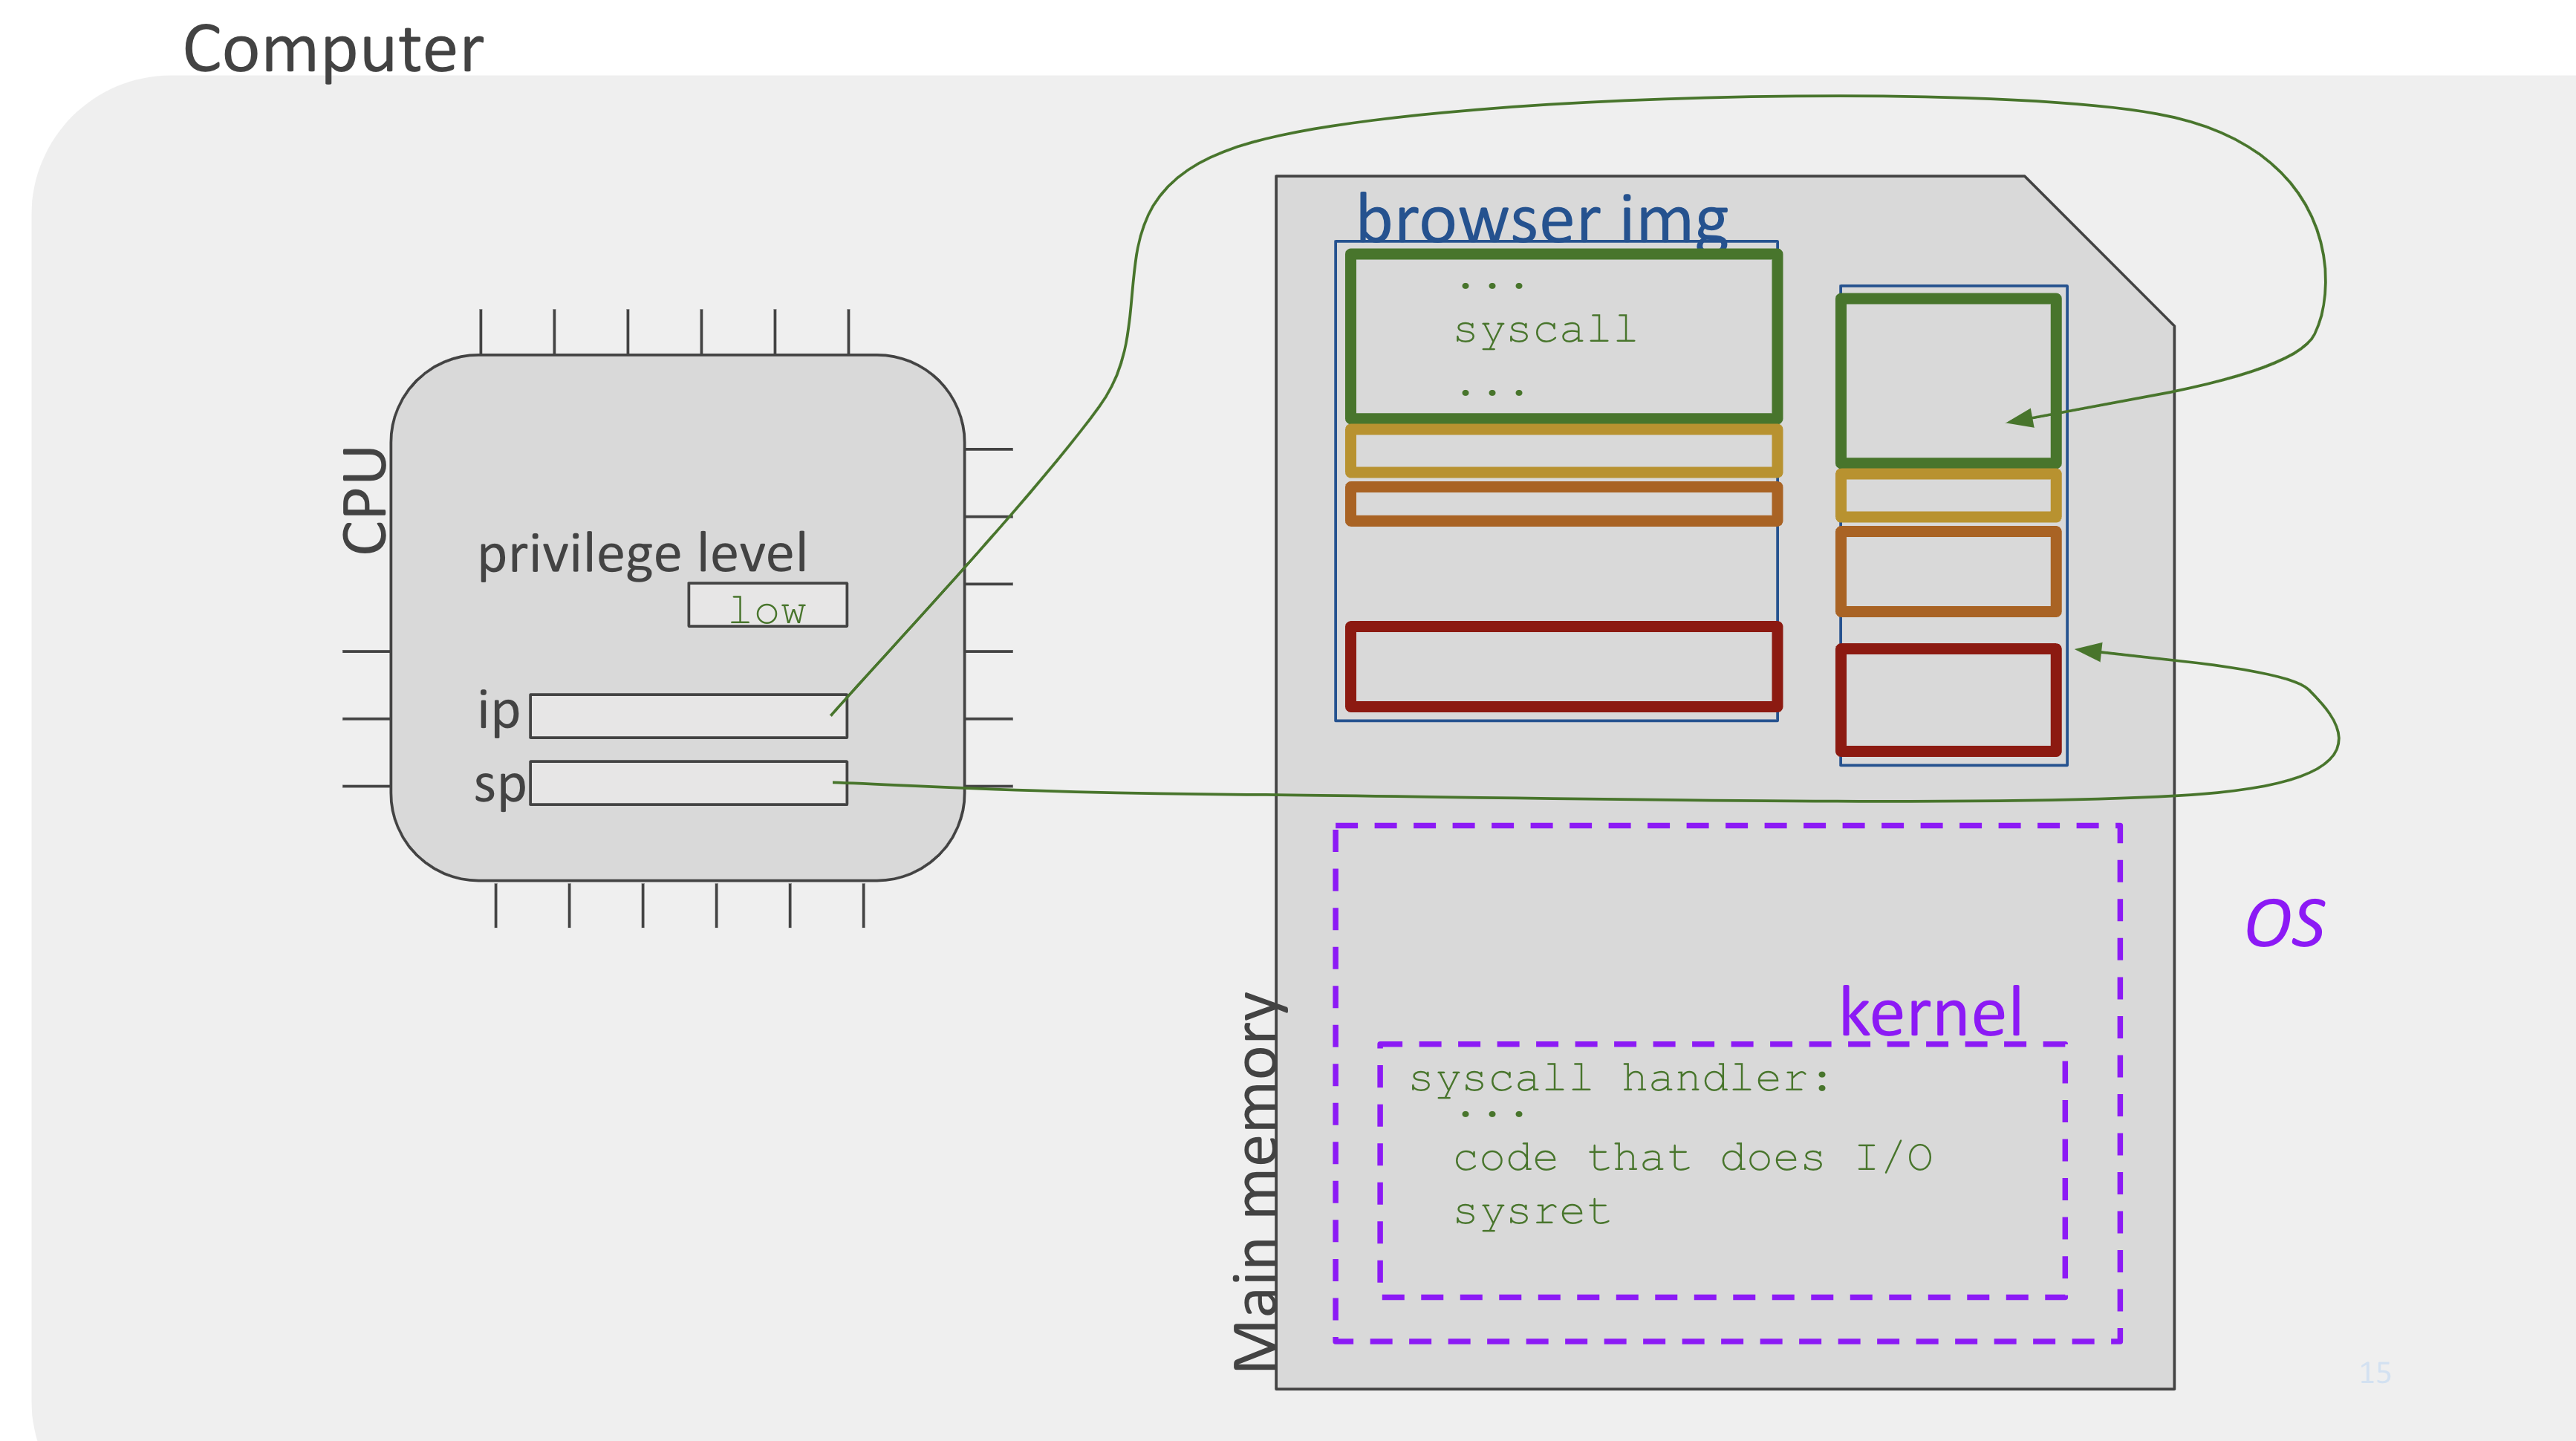
\includegraphics[width=0.8\textwidth]{chapters/L3/images/parallel-syscall.png}
\end{center}
\newpage
\subsection{Process I/O and Scheduling}
When a process initiates an I/O operation:\\
\begin{minipage}[htp]{0.45\textwidth}
\begin{itemize}
  \item It transitions from \emph{Running} to \emph{Blocked} as it waits for the I/O to complete.
  \item Once the I/O is complete, the process moves to the \emph{Ready} state.
  \item The OS scheduler then selects processes from the Ready queue to run, ensuring fair CPU utilization.
\end{itemize}
\end{minipage} 
\hfill 
\vline 
\hfill 
\begin{minipage}[htp]{0.45\textwidth}
\begin{center}
  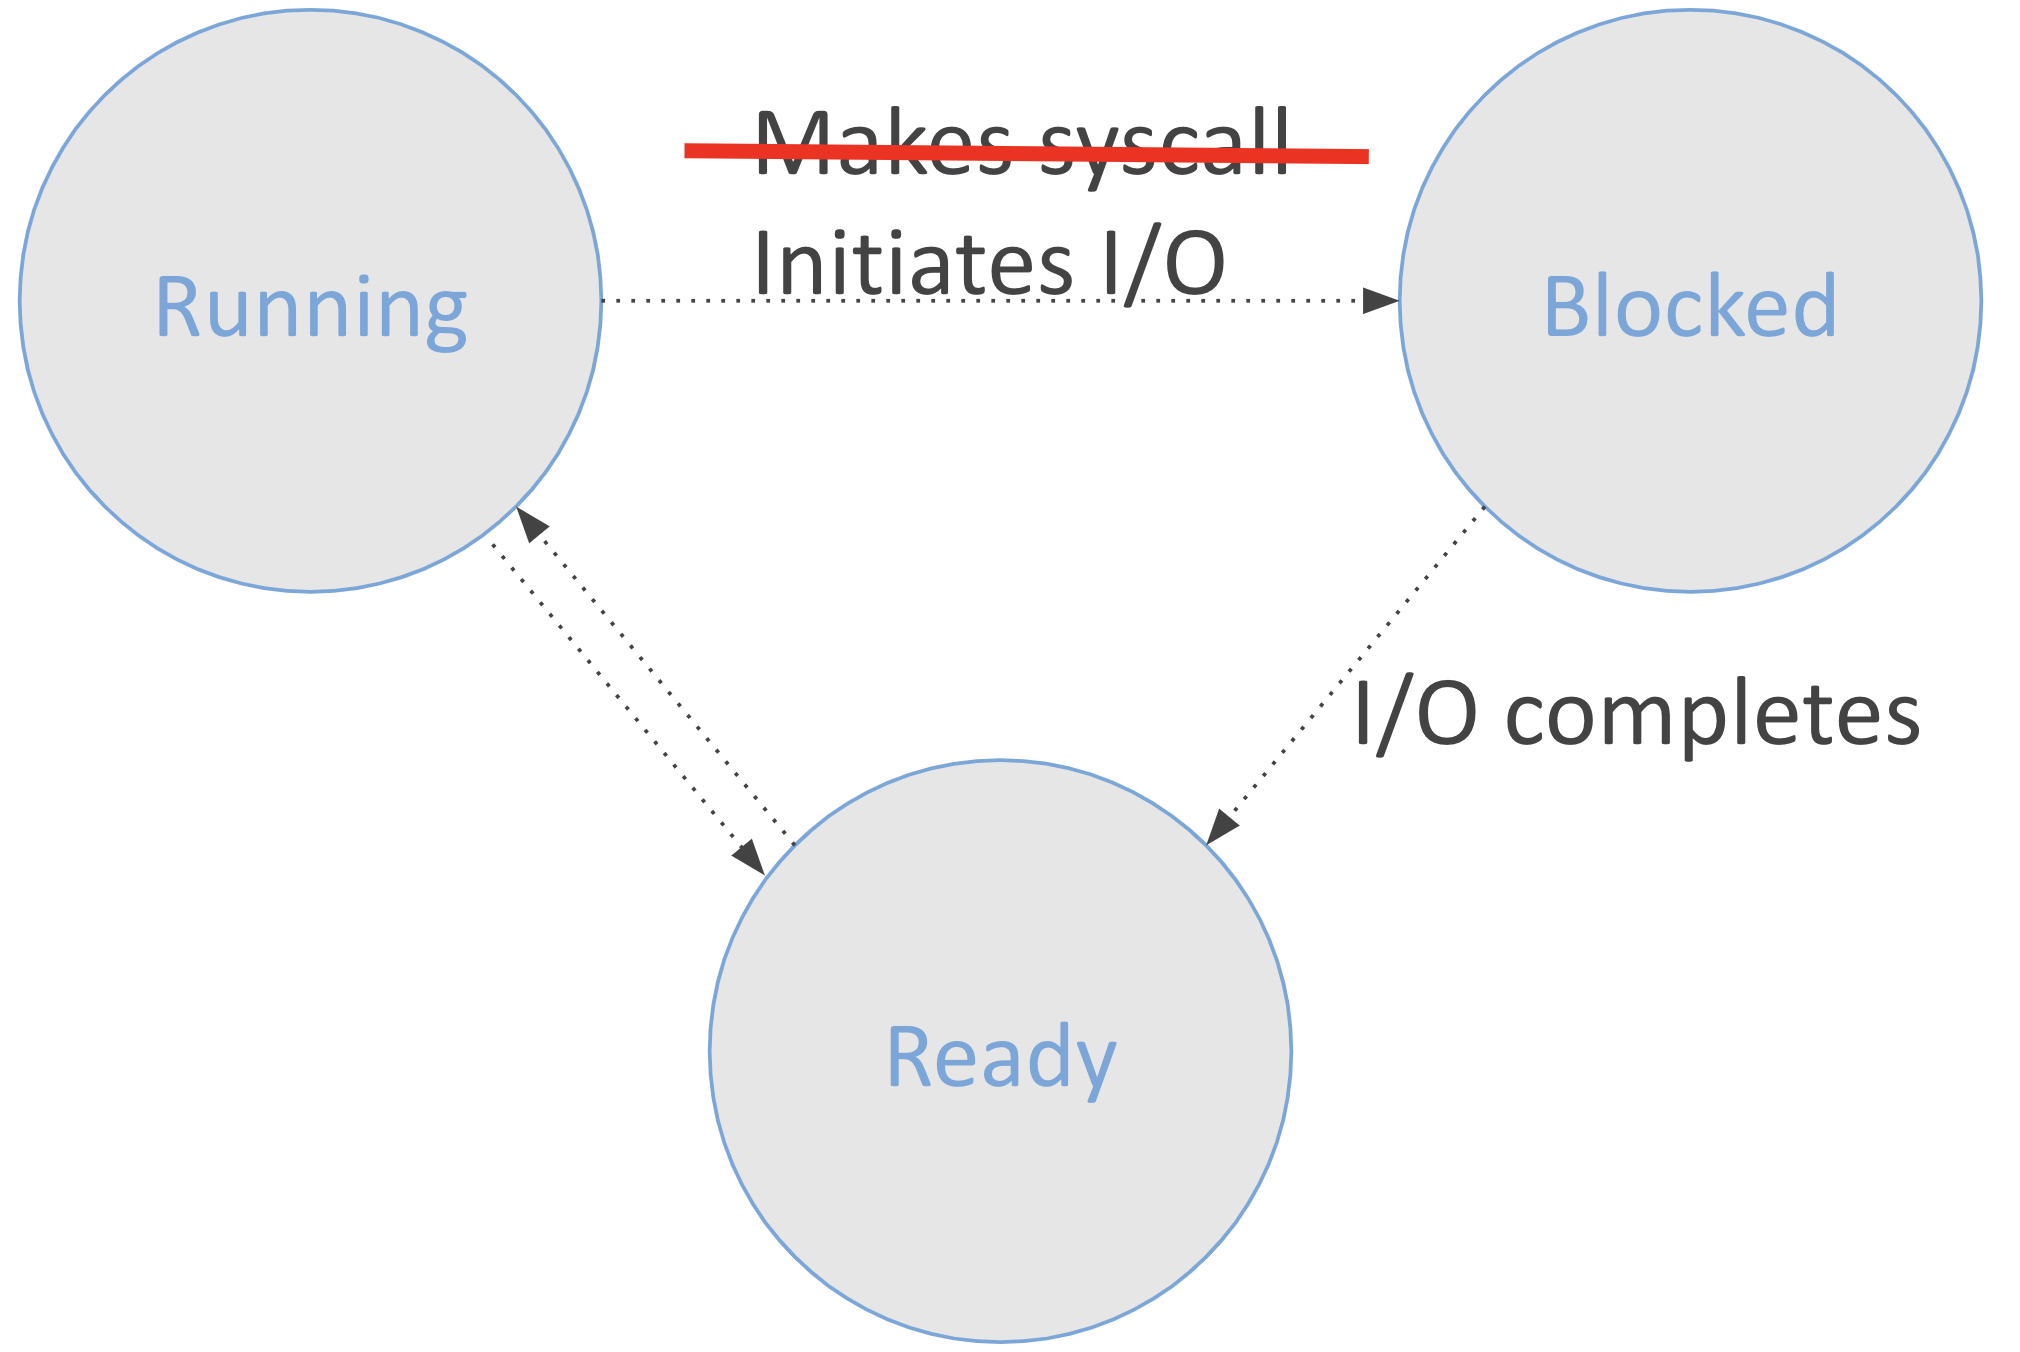
\includegraphics[width=0.95\textwidth]{chapters/L3/images/diagram.png}
\end{center}
\end{minipage}
\vspace{20px}
\section{The Kernel's Job cont.}
The Kernel handles several types of events:
\begin{itemize}[topsep=3px]
  \item[-] \textbf{Syscalls:} Requests from running threads for system-level services.
  \item[-] \textbf{Exceptions/Traps:} Synchronous signals generated when a thread executes an illegal or erroneous operation (e.g., division by zero).
  \item[-] \textbf{Interrupts:} Asynchronous signals from external devices (e.g., mouse events, network packets) requiring immediate attention.
\end{itemize}
\vspace{10px}
\begin{minipage}[htp]{0.45\textwidth}
\subsubsection*{Exception Handling}
\textit{What happens if the browser executes unauthorized code or encounters an error, such as dividing by zero ?}\\
When a process executes an illegal operation, the CPU raises an exception. The kernel then takes over to handle the error safely.
\vspace{8px}
\begin{center}
  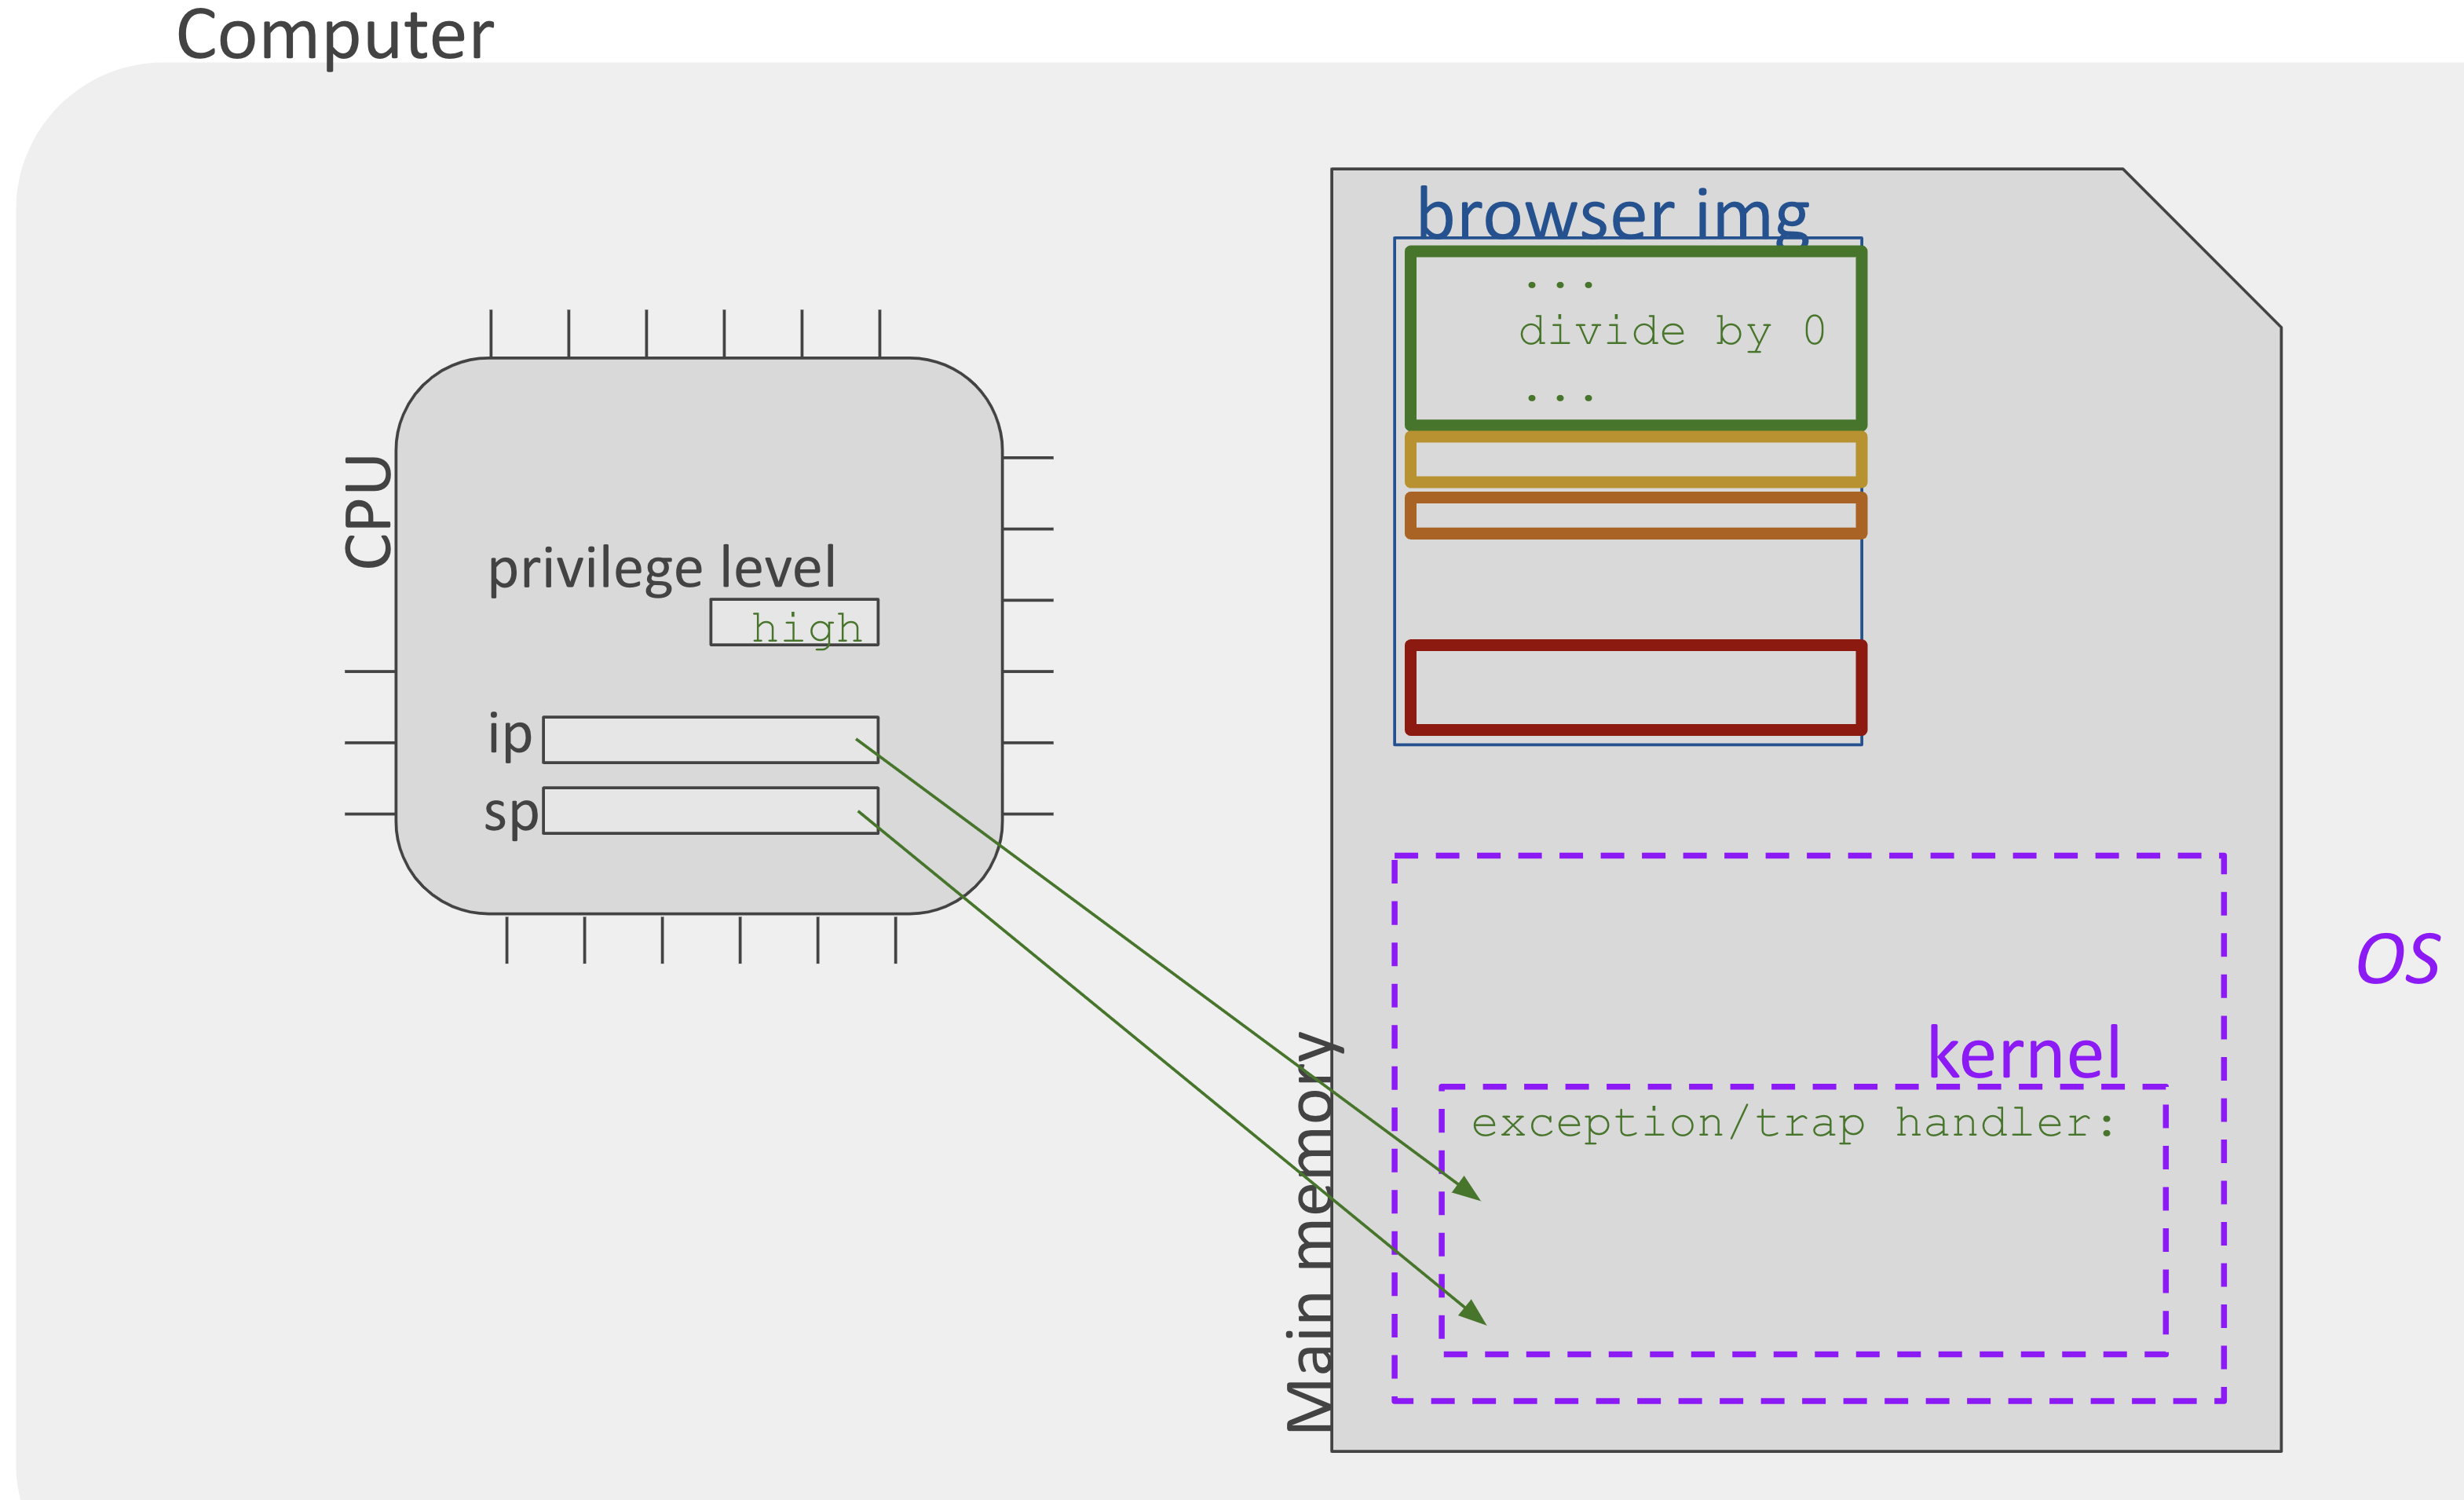
\includegraphics[width=0.95\textwidth]{chapters/L3/images/exception.png}
\end{center}
\end{minipage} 
\hfill 
\vline 
\hfill 
\begin{minipage}[htp]{0.45\textwidth}
\subsubsection*{Interrupt Handling}
Interrupts are triggered by external events and are managed by both hardware and software. The hardware raises the interrupt, and the kernel (via an interrupt handler) processes it.
\vspace{8px}
\begin{center} 
  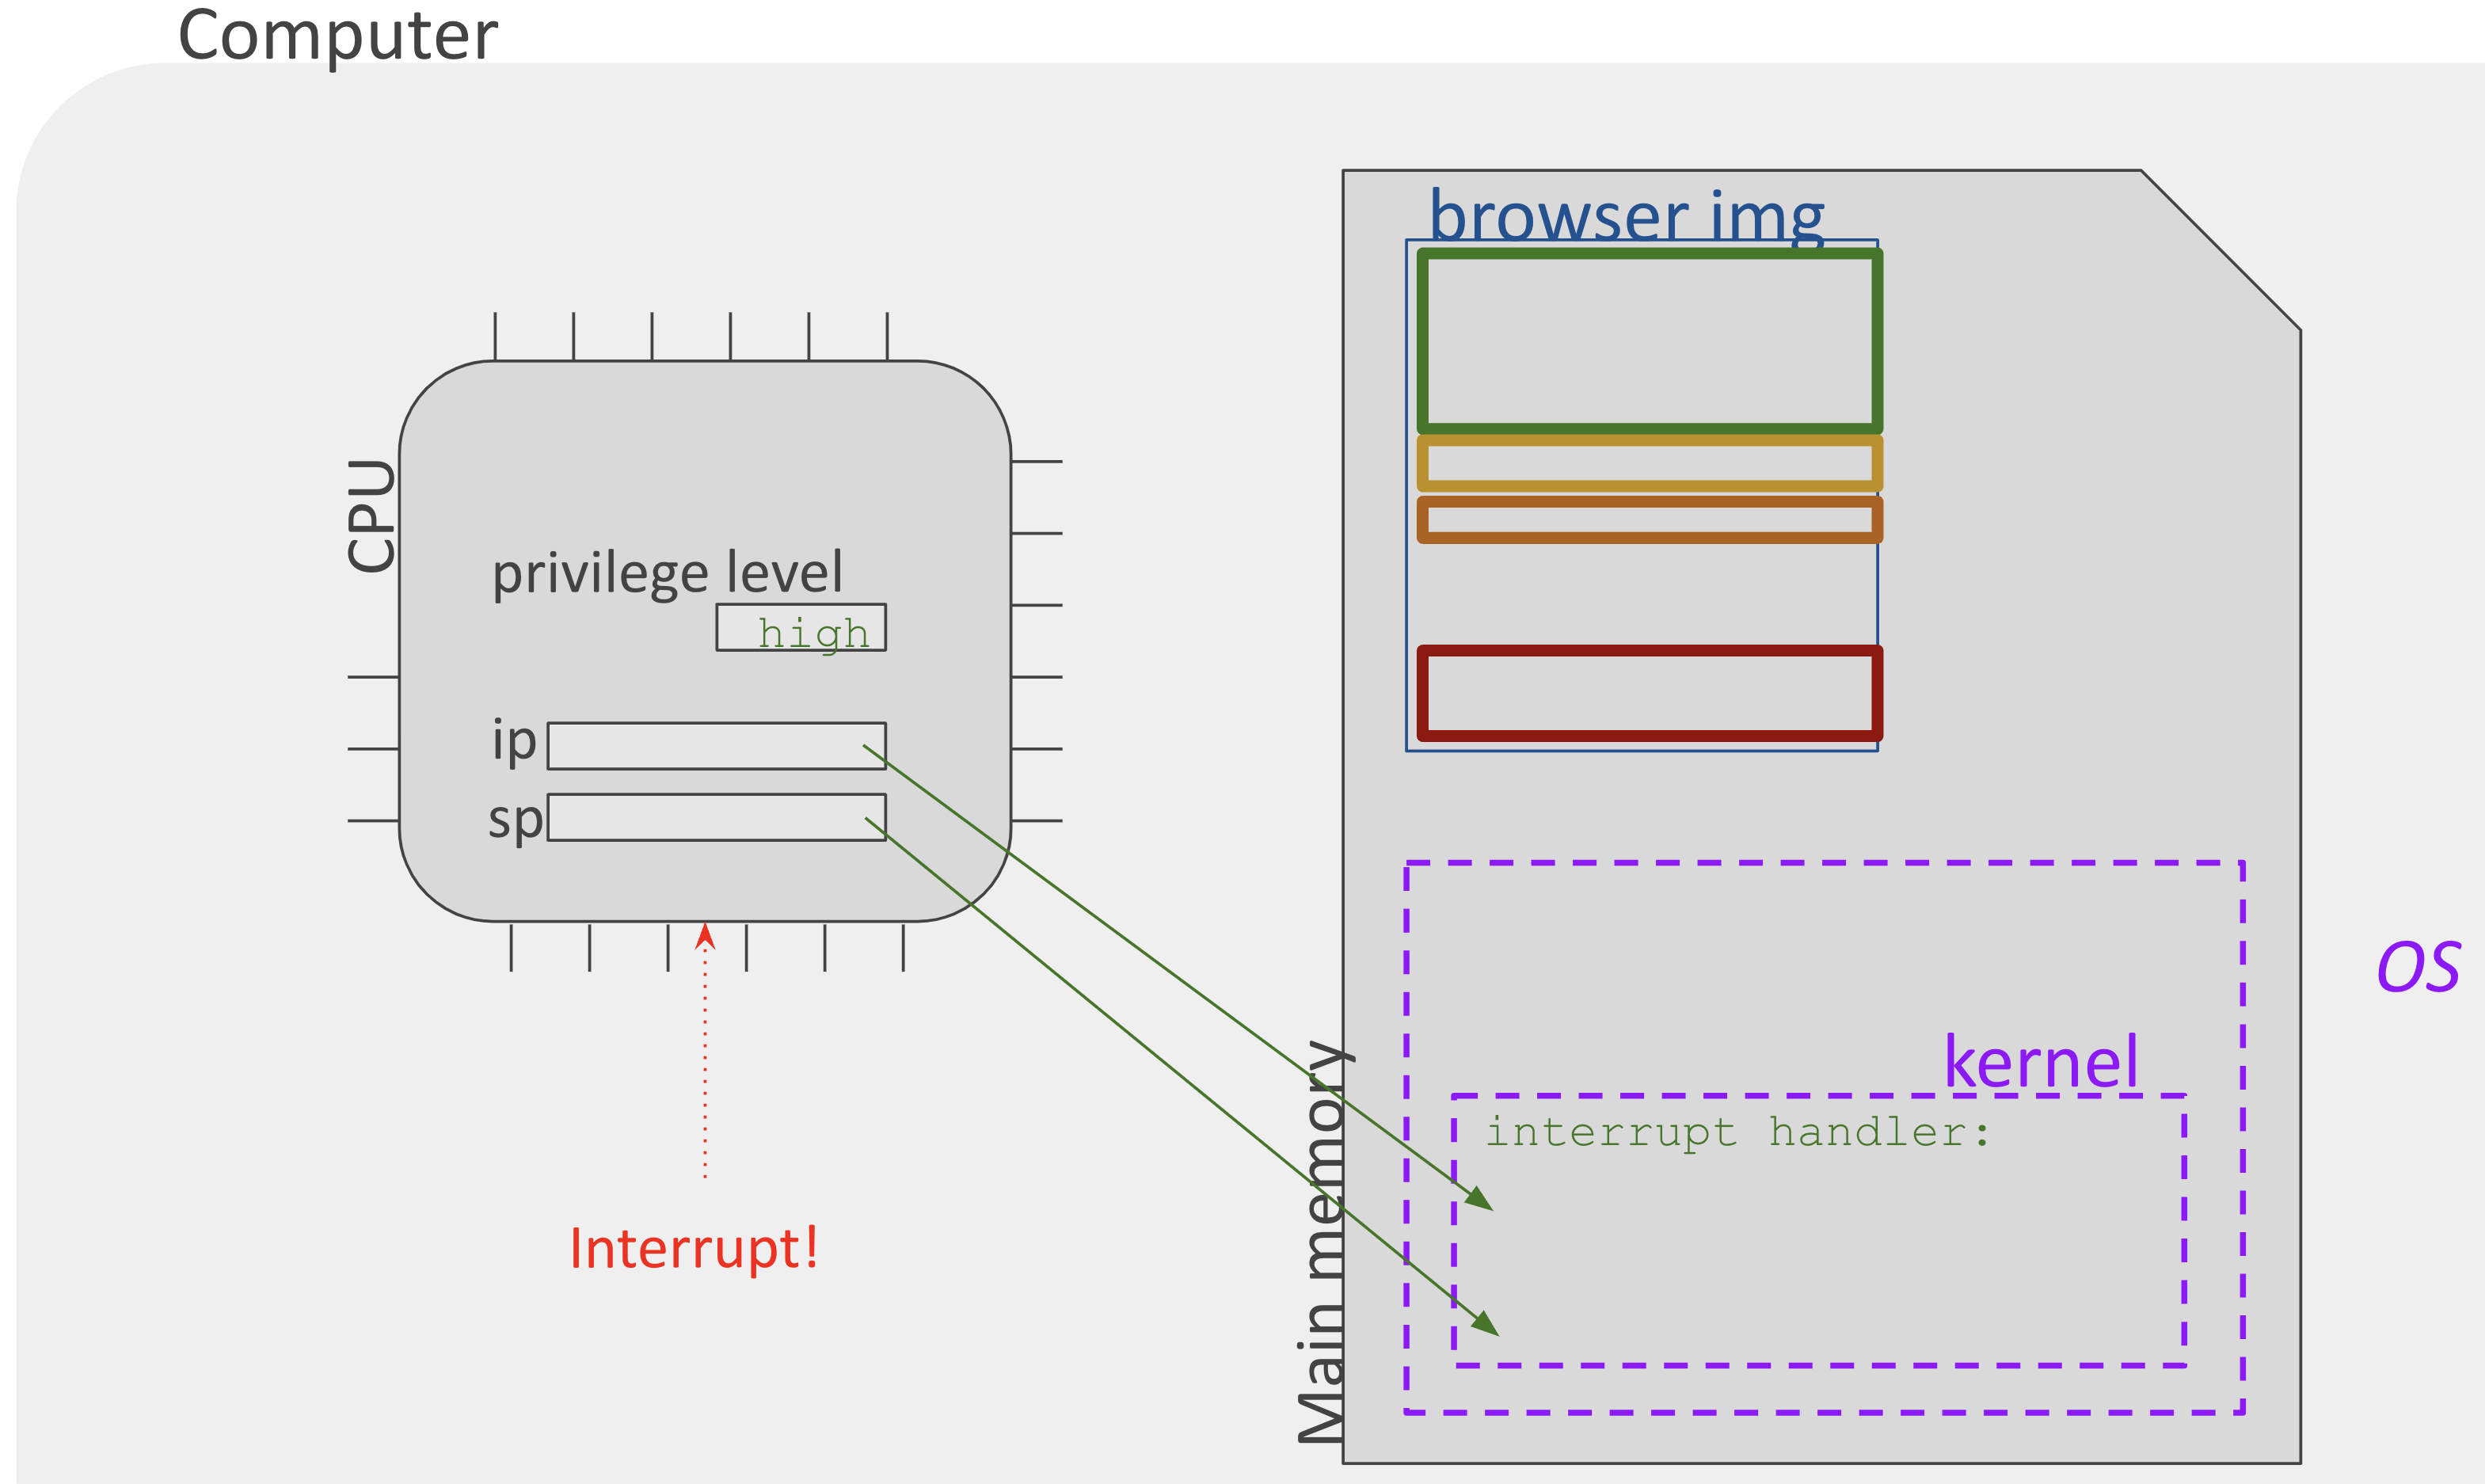
\includegraphics[width=0.95\textwidth]{chapters/L3/images/interrupt.png}
\end{center}
\end{minipage}

\subsubsection{The Timer Interrupt}
\begin{definition}[Timer Interrupt]
The timer interrupt is raised at regular intervals (typically every few milliseconds). Its handler invokes the OS scheduler to decide which process runs next, ensuring that no process monopolizes the CPU.
\end{definition}
\vspace{15px}
\newpage
\subsubsection{The OS Scheduler}
The OS scheduler manages the state transitions of processes (Running, Blocked, Ready) based on various scheduling algorithms, thereby ensuring equitable CPU access.

\begin{center}
  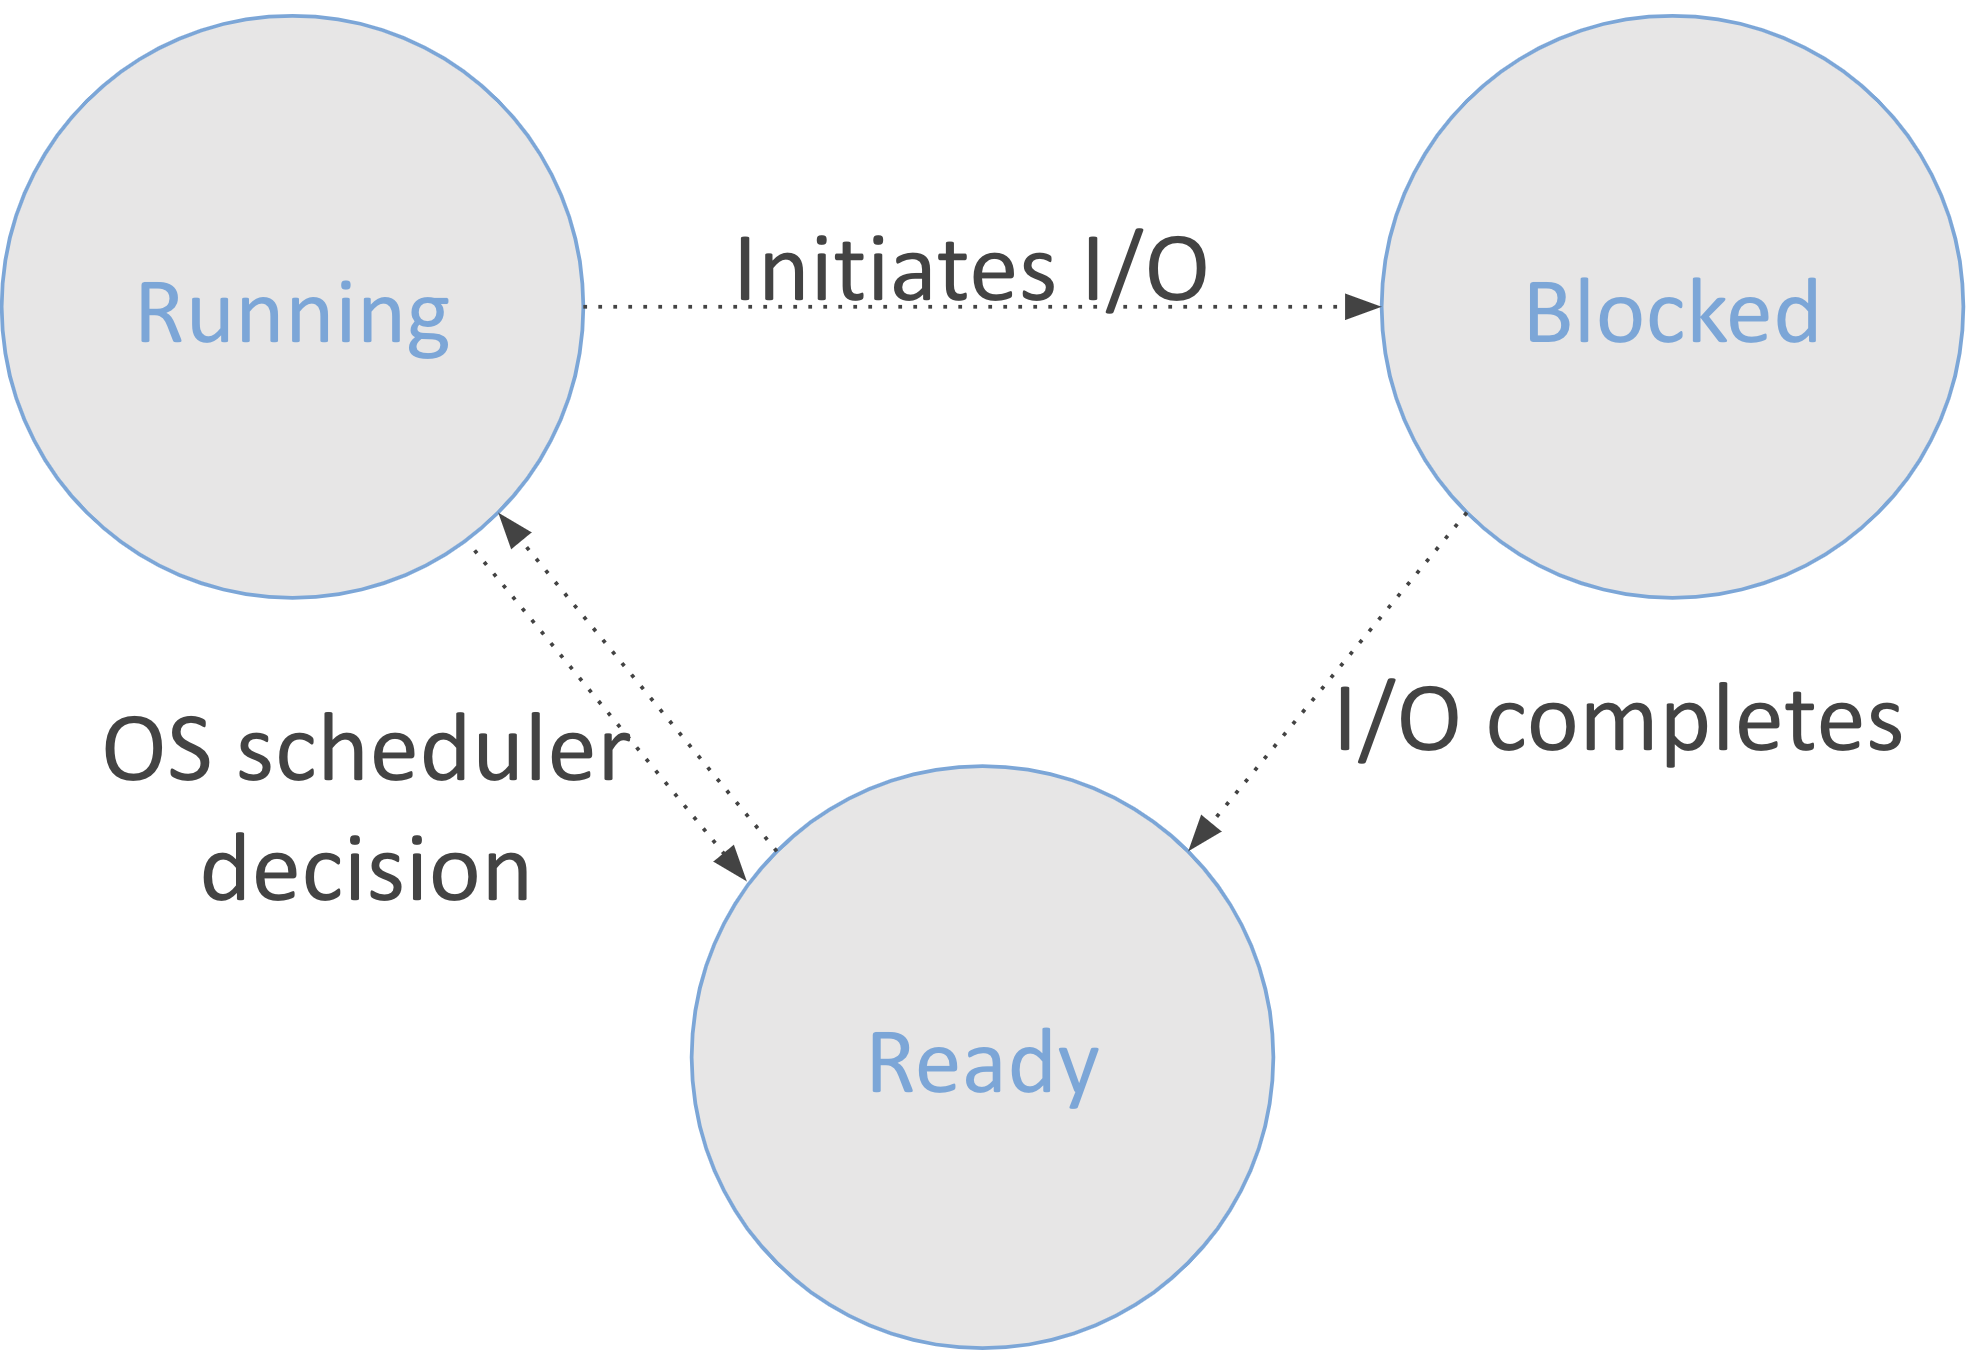
\includegraphics[width=0.45\textwidth]{chapters/L3/images/os-scheduler.png}
\end{center}

\subsection*{Summary - Limited Direct Execution}
\begin{itemize}
  \item[-] Normal threads execute in low privilege.
  \item[-] Operations requiring high privilege are performed via syscalls, exceptions, or interrupts, which invoke the kernel.
  \item[-] Timer interrupts ensure that the OS scheduler periodically gains control, maintaining fairness.
\end{itemize}

Limited direct execution is essential for safely and efficiently sharing the CPU among multiple processes.

\section{Executing Syscalls --- Process Management}

Processes are created, modified, and terminated using various syscalls. We now discuss the key syscalls involved in process management.

\subsection{Syscall Definitions}

\begin{definition}[Exit Syscall]
The \texttt{exit} syscall terminates a process. It never returns because, by the time control would return to the calling process, the process no longer exists.
\end{definition}

\begin{figure}[htp]
  \centering
  \begin{minipage}[htp]{0.45\textwidth}
\begin{cc}
_exit(0);
. 
. 
. 
. 
. 
. 
. 
. 
. 
. 
. 
\end{cc}
  \end{minipage}
  \hfill
  \vline
  \hfill
  \begin{minipage}[htp]{0.45\textwidth}
    \centering
    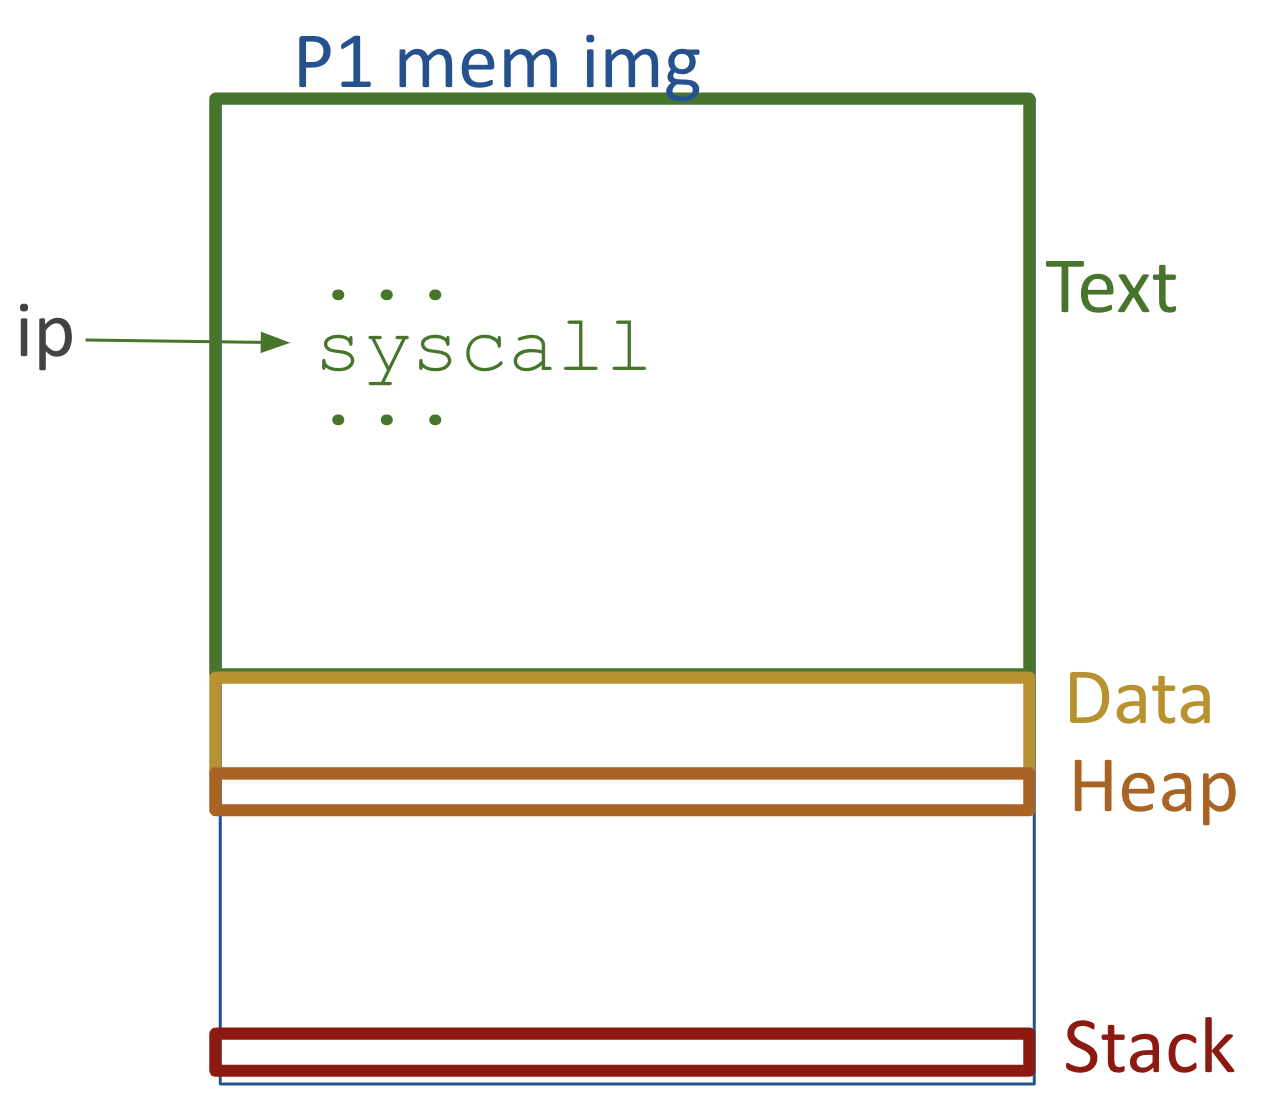
\includegraphics[width=0.8\textwidth]{chapters/L3/images/exit.png}
  \end{minipage}
  \caption{Exit Syscall: Code snippet and stack visualization.}
\end{figure}
\newpage
\begin{definition}[Exec Syscall]
The \texttt{exec} syscall replaces the current process image with a new program. It preserves the process ID and file descriptors while discarding the old program's code, data, and stack. On success, it does not return; on failure, it returns \texttt{-1}.
\end{definition}

\begin{figure}[htp]
  \centering
  \begin{minipage}[b]{0.45\textwidth}
    \begin{cc}
execvp("date", args);











    \end{cc}
  \end{minipage}
  \hfill
  \vline
  \hfill
  \begin{minipage}[b]{0.45\textwidth}
    \centering
    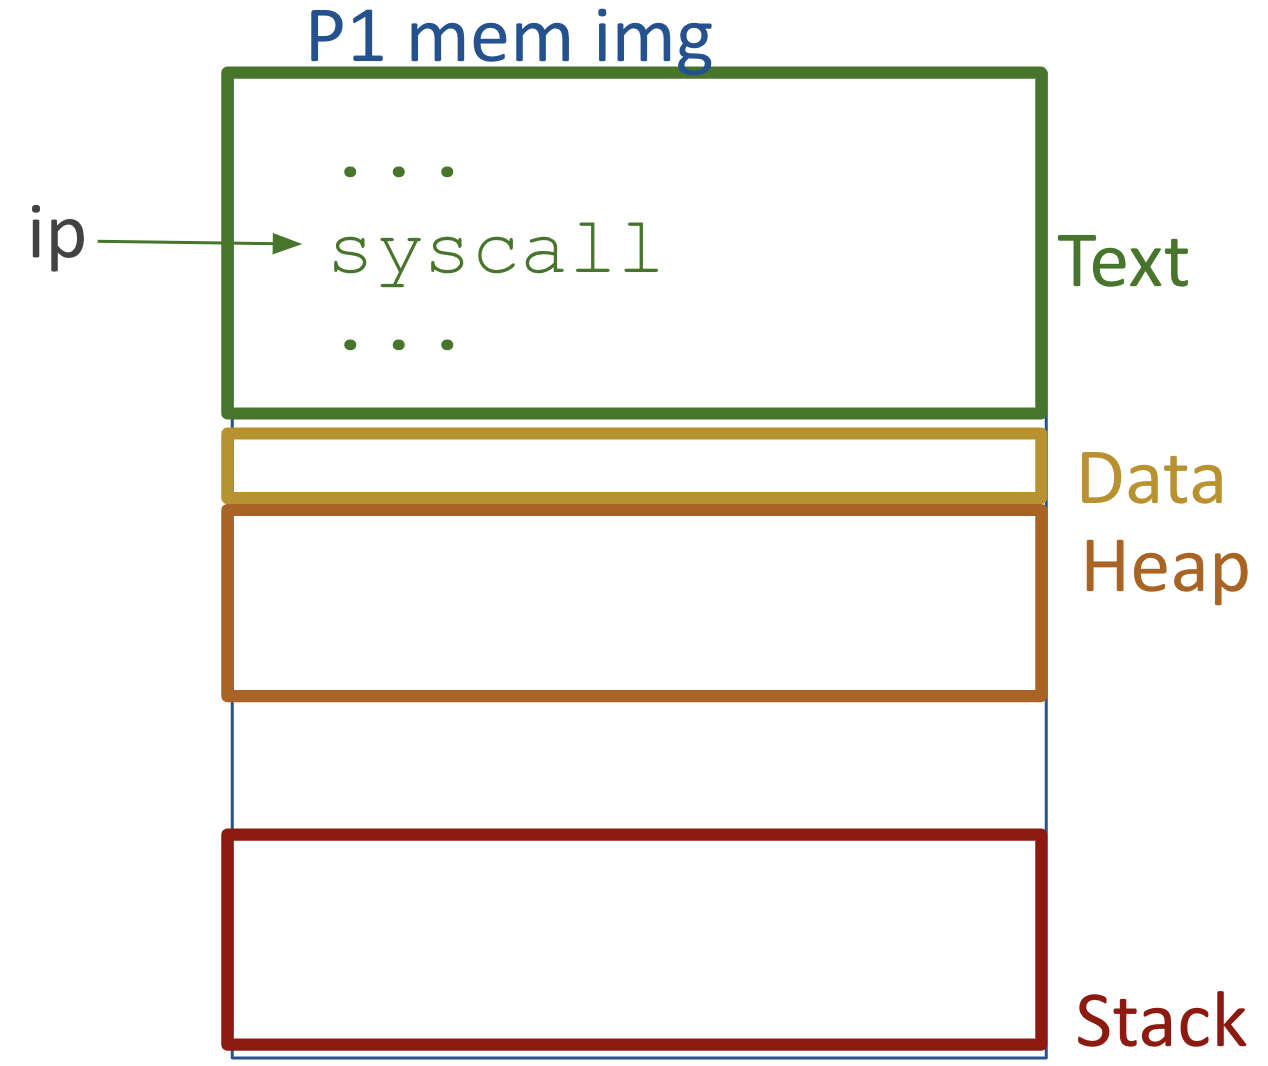
\includegraphics[width=0.8\textwidth]{chapters/L3/images/exec.png}
  \end{minipage}
  \caption{Exec Syscall: Code snippet and process image.}
\end{figure}

\begin{definition}[Fork Syscall]
The \texttt{fork} syscall creates a new child process by duplicating the calling process. Both the parent and child continue execution from the point of the fork, but in separate memory spaces. The fork returns \texttt{0} to the child and the child's process ID (PID) to the parent.
\end{definition}

\begin{figure}[htp]
  \centering
  \begin{minipage}[b]{0.45\textwidth}
    \begin{cc}
int fs = fork();
if (fs == 0) {
   // Child process code
} else {
   // Parent process code
}




    \end{cc}
  \end{minipage}
  \hfill
  \vline
  \hfill
  \begin{minipage}[b]{0.45\textwidth}
    \centering
    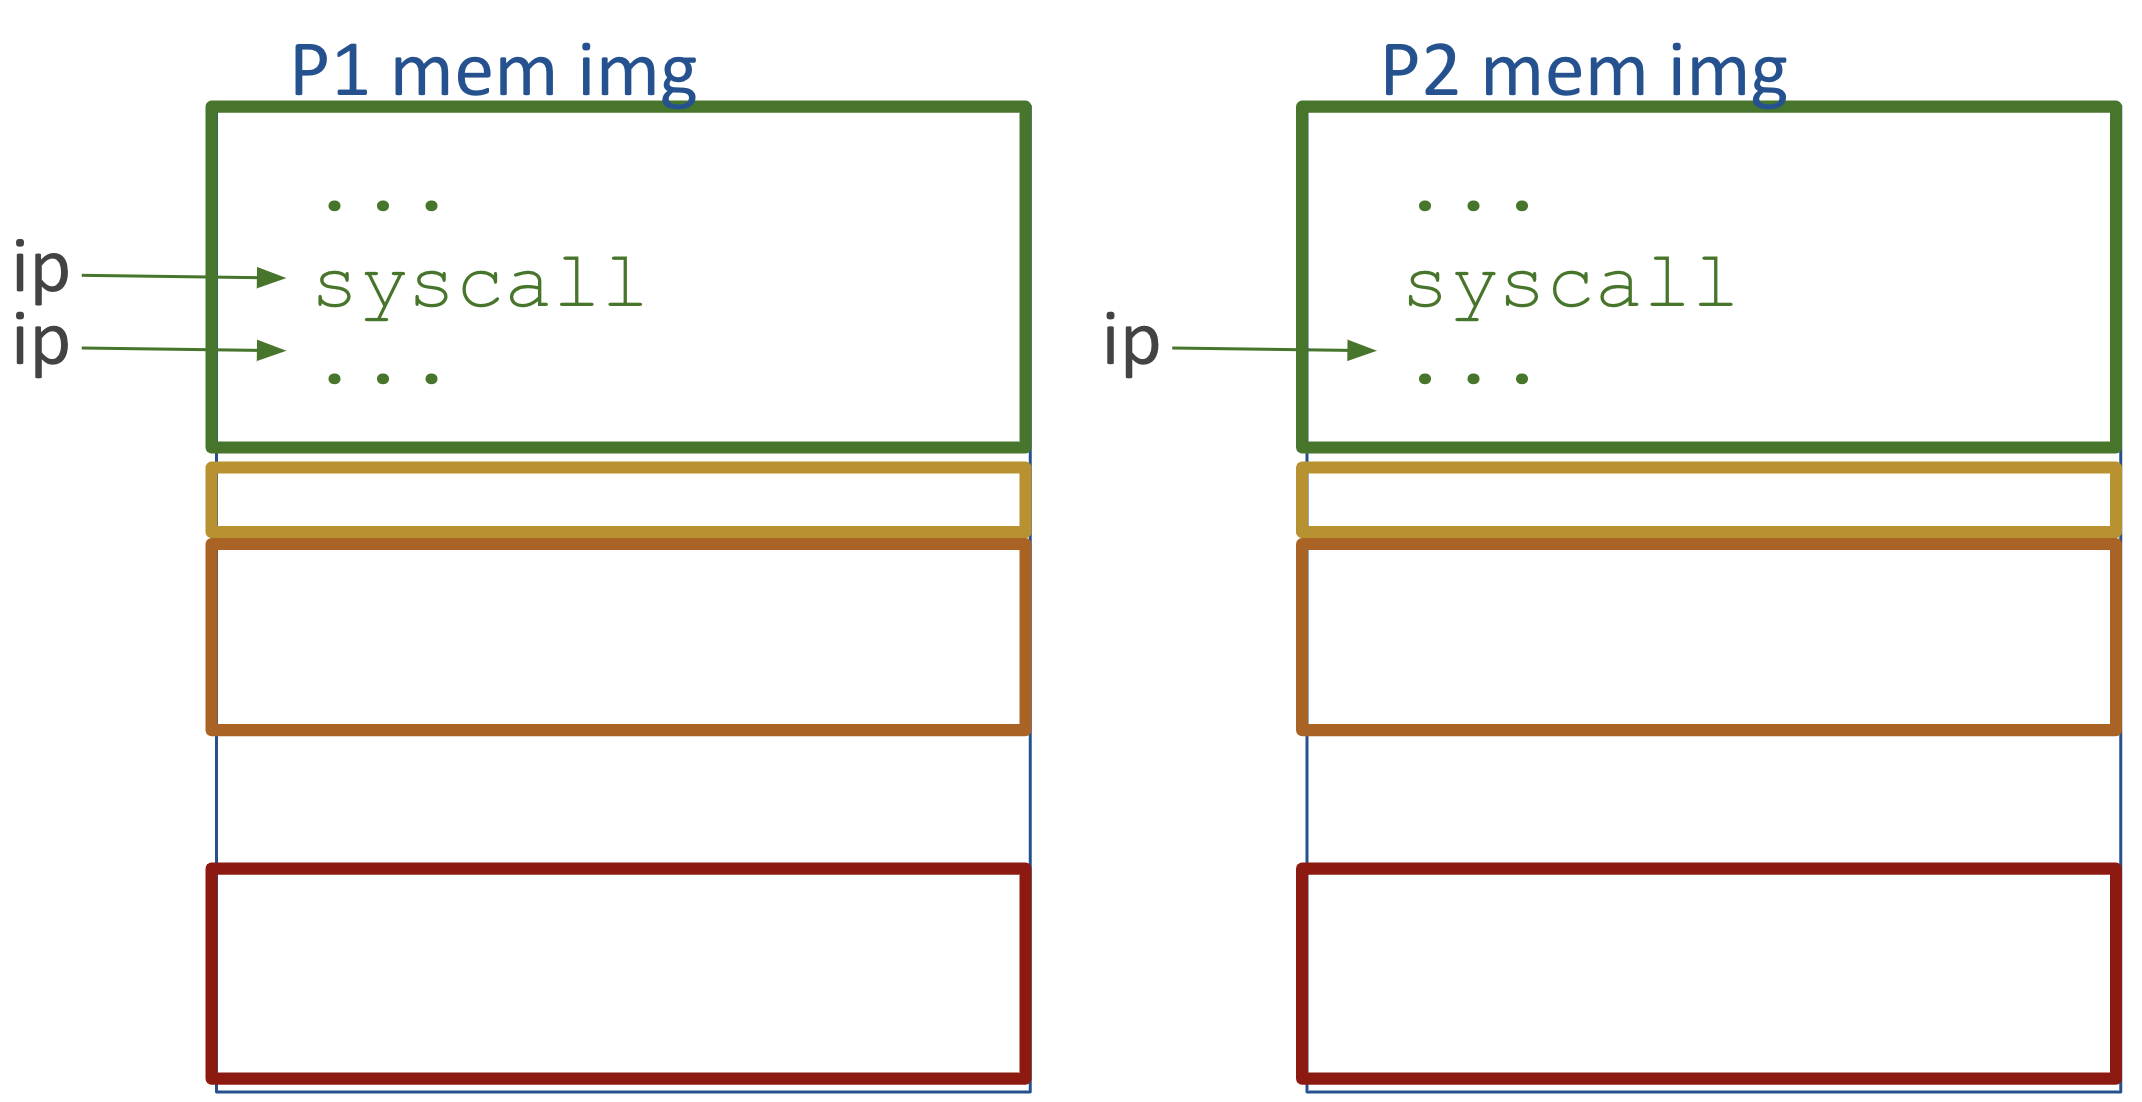
\includegraphics[width=1.25\textwidth]{chapters/L3/images/fork.png}
  \end{minipage}
  \caption{Fork Syscall: Example code and the resulting stack layout.}
\end{figure}

\begin{definition}[Wait Syscall]
The \texttt{wait} syscall allows a parent process to block until one of its child processes terminates. If no child process exists, \texttt{wait()} returns an error.
\end{definition}

\subsection{Process Creation and Cleanup}

Processes are typically created by combining the \texttt{fork} and \texttt{exec} syscalls. For example:
\begin{cc}
int fs = fork();
if (fs == 0) {
   execvp("date", args);
} else {
   wait(fs);
}
\end{cc}

When a parent process calls \texttt{wait()}, it is blocked until a child terminates, ensuring proper cleanup of child processes.
\newpage
\section{The OS Process Graph}
The OS maintains a process graph where each square represents a process and each arrow indicates the parent-child relationship. These kind of graphs are crucial for understanding process creation and hierarchy.

\begin{center}
  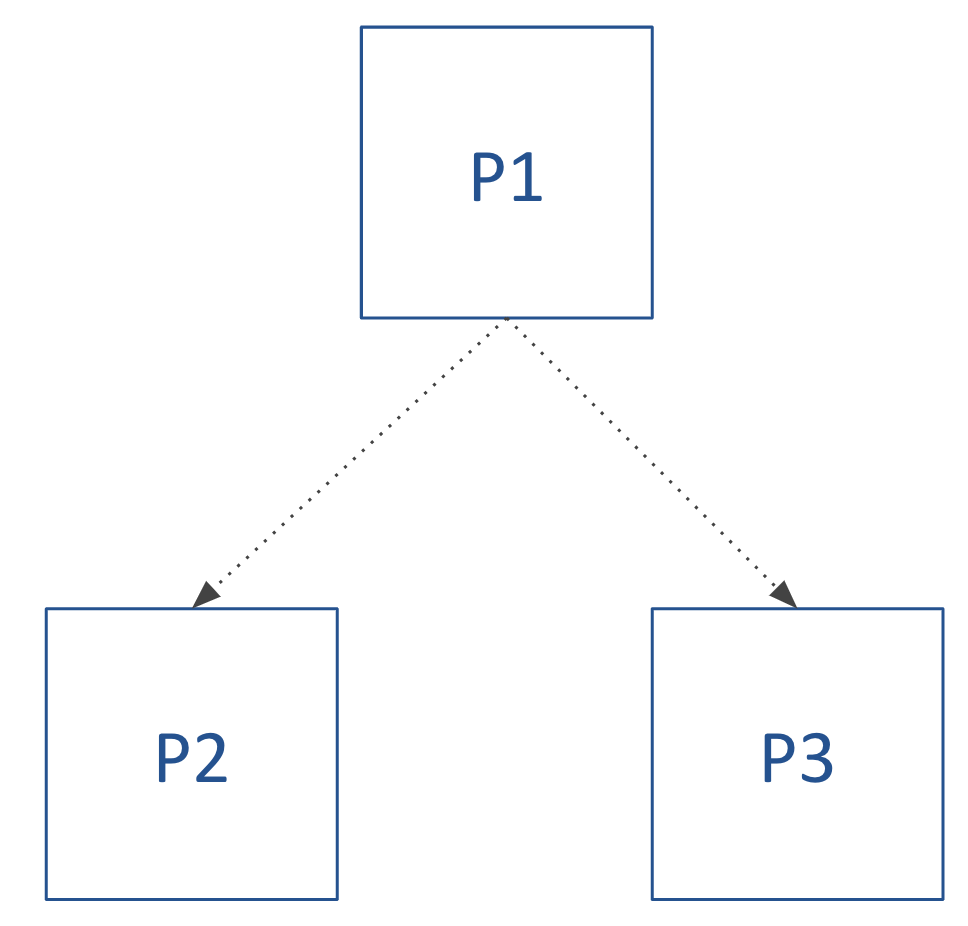
\includegraphics[width=0.25\textwidth]{chapters/L3/images/graph.png}
\end{center}

\section{Key Processes in the OS}

Some critical processes managed by the OS include:
\begin{itemize}
  \item[-] \textbf{GUI Processes:} Manage the graphical user interface.
  \item[-] \textbf{Terminal Processes:} Handle command-line interactions.
  \item[-] \textbf{Init Process:} The first process created by the kernel, responsible for starting system services.
  \item[-] \textbf{Idle Process:} Executes when no other process is runnable.
\end{itemize}

\subsection*{Conclusion - The Role of Syscalls}

Syscalls provide the interface through which processes access system resources such as storage and networks. They also facilitate self-management operations, including process creation, modification, and cleanup. Through mechanisms such as limited direct execution, exceptions, and interrupts, the OS ensures that the CPU is shared safely and efficiently among all processes.
 
\documentclass[../../compsys.tex]{subfiles}
\begin{document}
\chapter{L4 - Memory}
\textit{This chapter covers the fundamentals of main memory, process memory images, memory virtualization, and the CPU's role in managing memory.}
\vspace{15px}
\section{Main Memory}
Main memory is conceptualized as a linear array of bytes, where each byte has a unique memory address (e.g., \texttt{0x0}, \texttt{0x1}, \texttt{0x2}, etc.). Each byte can store any value that fits within its 8-bit capacity, and importantly, the value stored in a given byte is independent of its memory address. For instance, the byte at address \texttt{0x0} may contain the value 8, 0, or any other valid 8-bit number.

\subsection{Memory Operations by the CPU}
The CPU interacts with main memory by executing specific instructions to read from and write to it. These operations are fundamental to both data processing and code execution:

\begin{itemize}
  \item[-] \textbf{Read Operation:} The CPU issues an instruction to read a block of bytes (for example, 8 bytes starting at address \texttt{0x0}) and loads the result into a register (such as \texttt{rax}).
  \item[-] \textbf{Write Operation:} The CPU executes an instruction that writes data from a register (e.g., \texttt{rax}) into a block of memory (for example, starting at address \texttt{0xb}).
\end{itemize}

Although main memory stores only numbers, the CPU interprets these numbers differently depending on whether they represent data (such as variables) or executable code (such as the instruction \texttt{mov rax, [0x0]}).

\begin{center}
  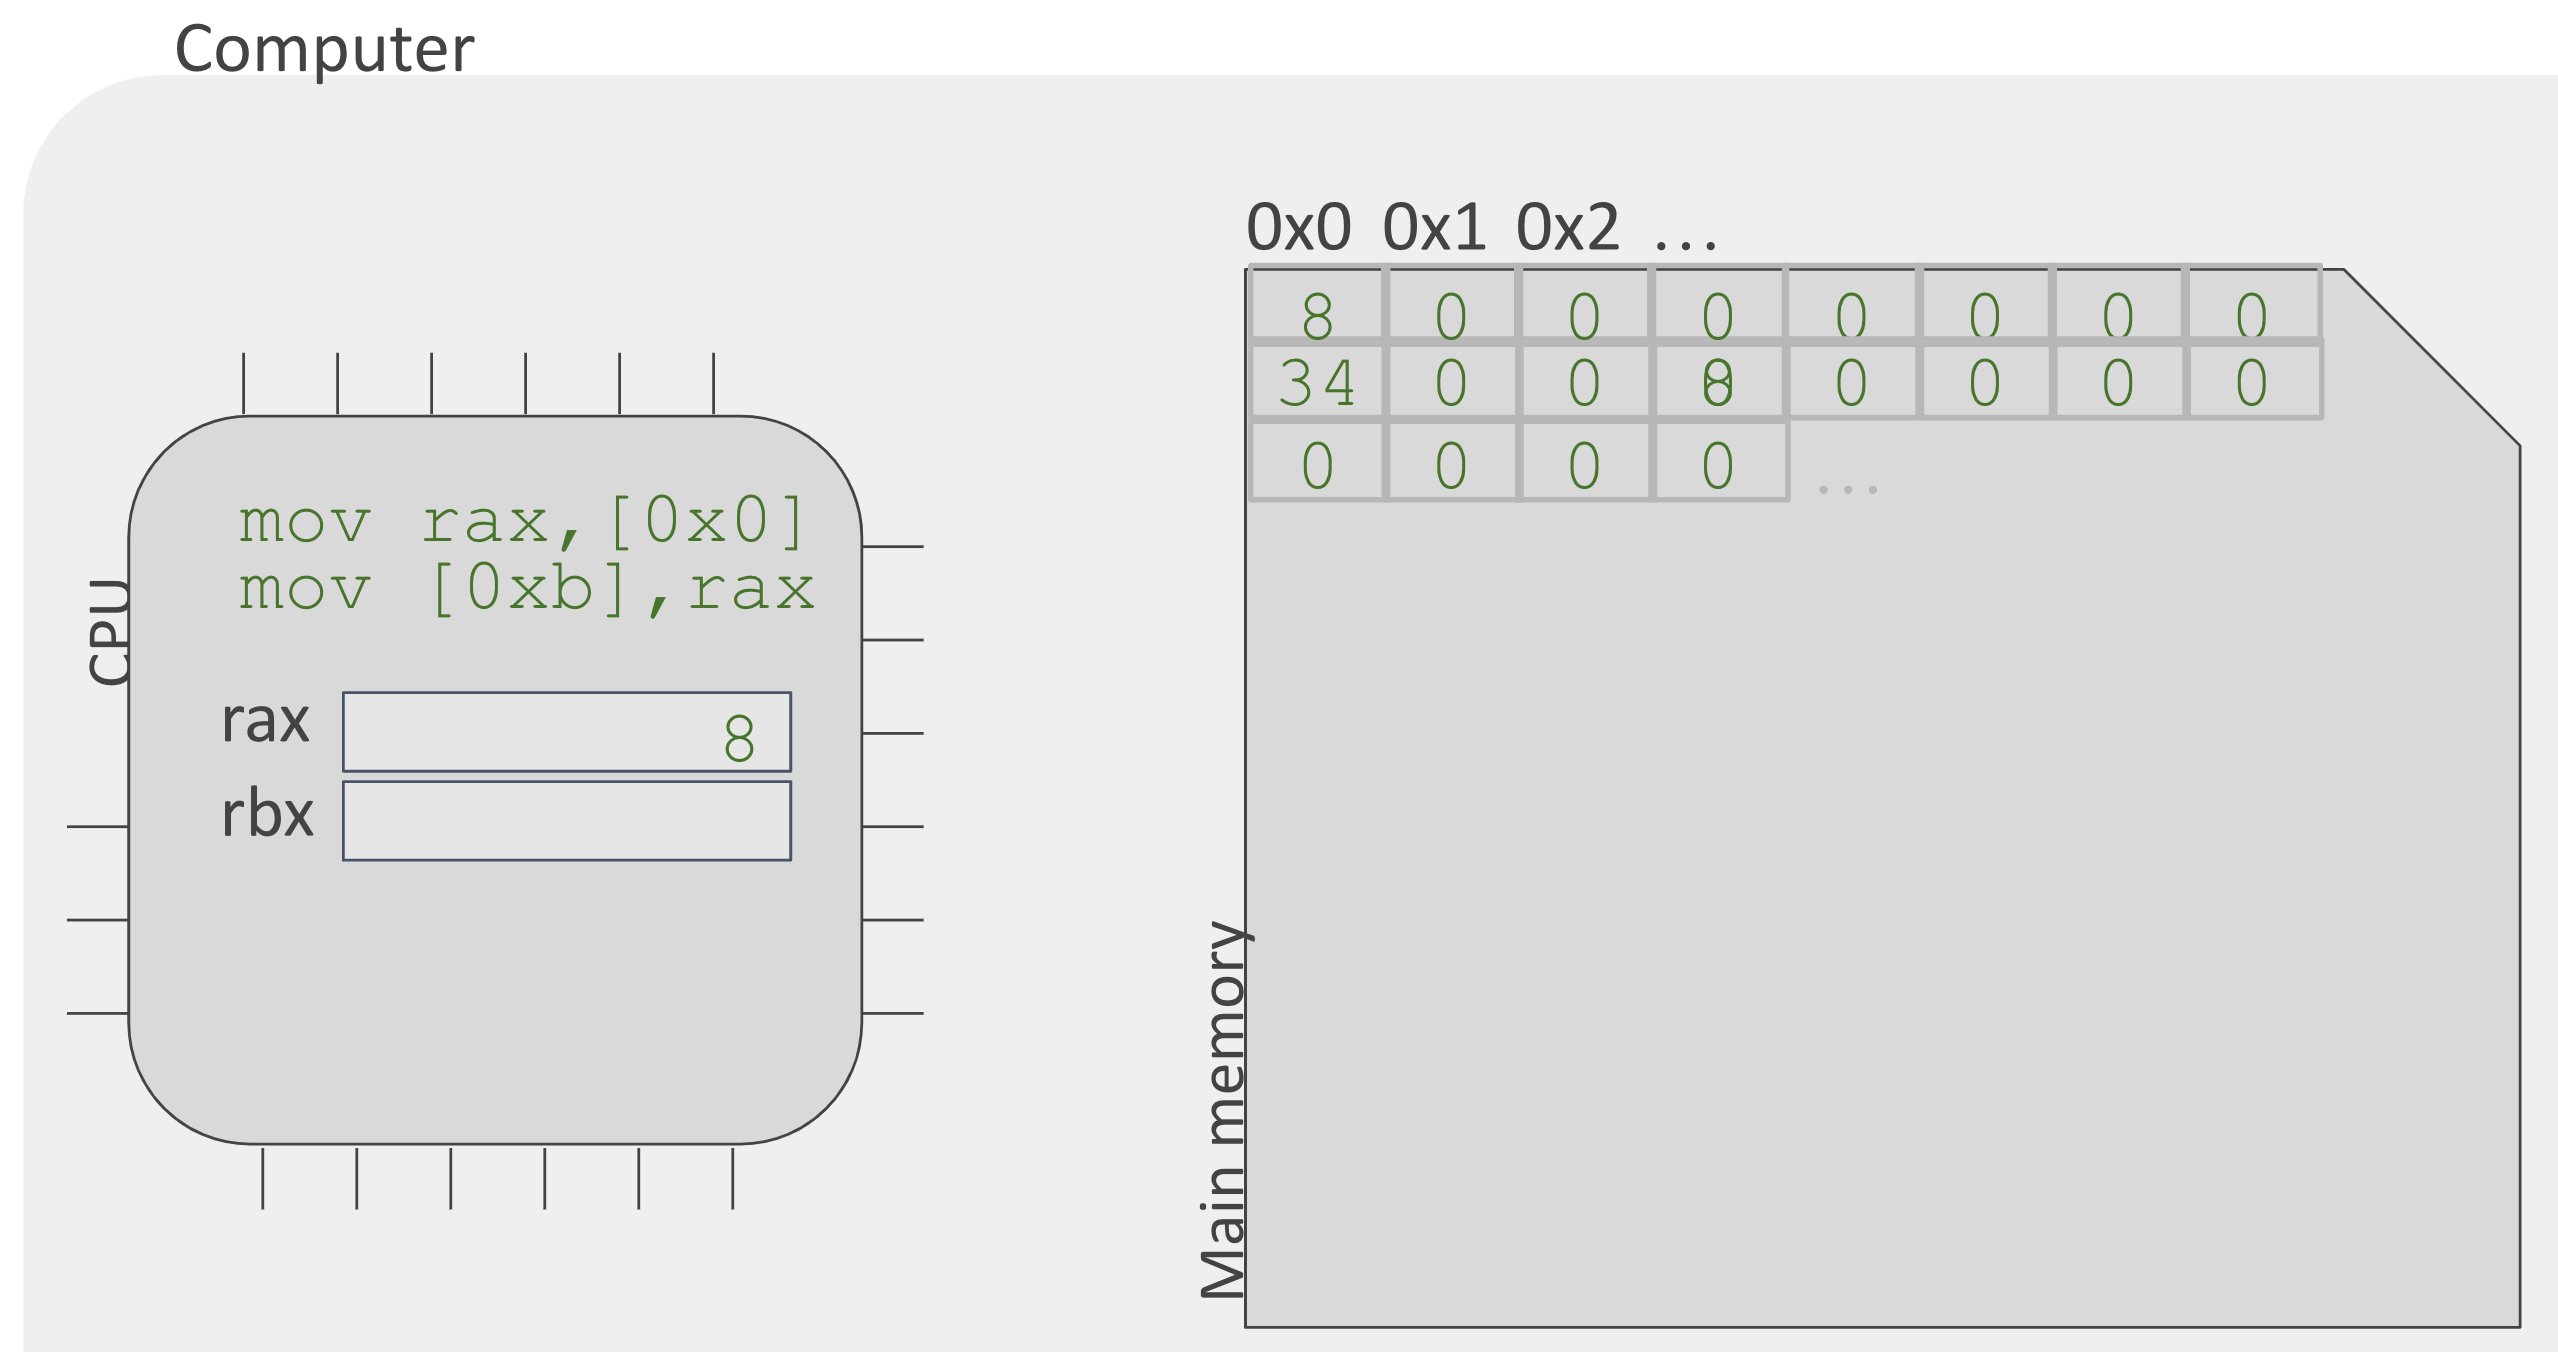
\includegraphics[width=0.45\textwidth]{chapters/L4/images/main-mem.png}
\end{center}
\newpage
\subsection{Instruction Pointer}
A key component in the CPU's control mechanism is the \emph{instruction pointer} (IP), in some contexts (ie. FDS, Comparch), this register is also known as the \emph{program counter} (PC), but the term "instruction pointer" more precisely describes its function.
\vspace{10px}
\begin{definition}[Instruction Pointer]
\leavevmode\\[5px]
The \textbf{instruction pointer} is a CPU register that holds the memory address of the next instruction to be executed.
\end{definition}
\vspace{5px}
\subsection{Subparts of Main Memory}
Main memory contains not only the memory images of individual processes but also the code and data essential to the operating system (OS). The OS comprises several critical components that ensure the proper operation and usability of the computer. These components include:

\begin{itemize}
  \item \textbf{Process Memory Images:} Every process has its own memory image, typically divided into:
  \begin{itemize}
    \item \textbf{Data Segment:} Stores global variables.
    \item \textbf{Stack Segment:} Contains local variables, return addresses, and other function call-related data.
    \item \textbf{Heap Segment:} Holds dynamically allocated memory (e.g., allocated via \texttt{malloc}).
  \end{itemize}
  \vspace{5px} 
  \item \textbf{Operating System Code:} This comprises all the code necessary for the computer's operation and usability. OS code is organized into:
    \begin{itemize}
      \item \emph{Kernel:} The central component of the OS, running in high-privilege mode. It manages system resources, hardware interactions, and security, ensuring the core functions of the computer operate correctly. It is neither a process nor a library (end of lecture explains).
        \begin{itemize}
          \item It creates and deletes processes and threads.
          \item It initiates I/O.
          \item It handles errors and interrupts.
          \item It decides which thread will run next.
        \end{itemize}
      \item \emph{Processes:} Such as the graphical user interface (GUI) and terminal applications, which provide user-level interaction with the system.
      \item \emph{Libraries:} Modules like the standard C library that provide a suite of functions, which are dynamically integrated into processes when called.
    \end{itemize}
\end{itemize}

\begin{center}
  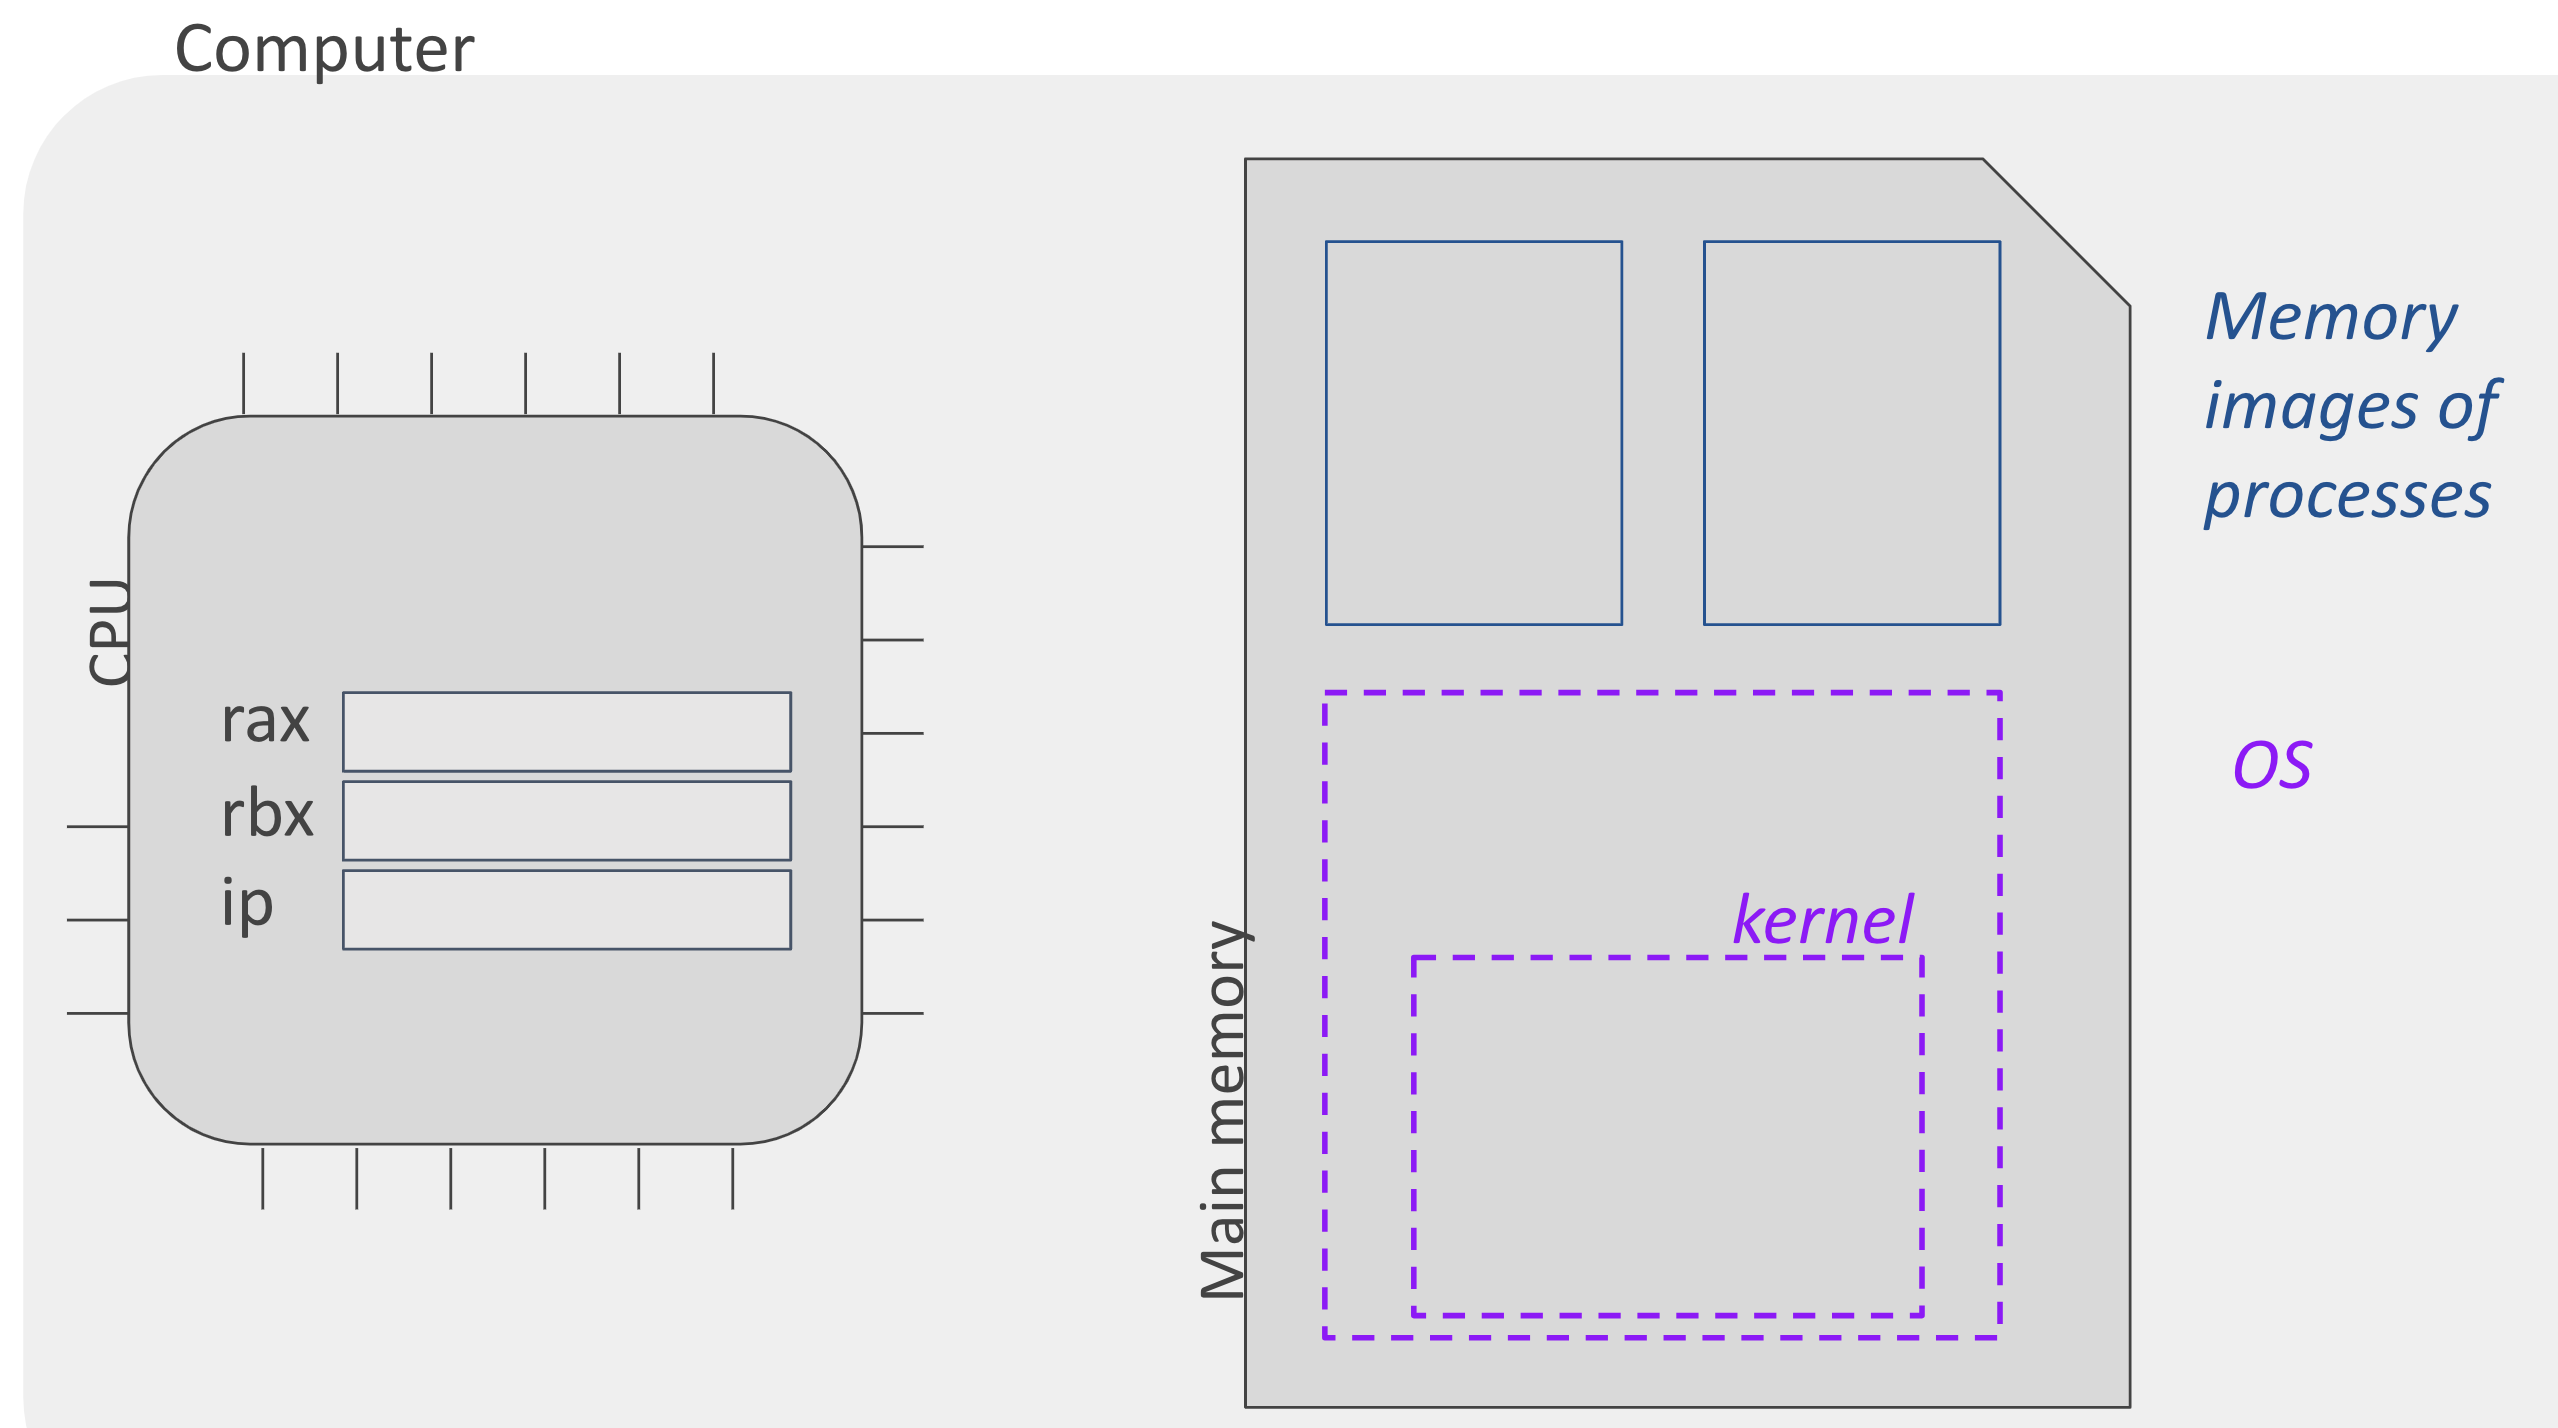
\includegraphics[width=0.45\textwidth]{chapters/L4/images/main-mem-content.png}
\end{center}
\newpage
\section{Process Memory Image}
\begin{definition}[Process Memory Image]
  \leavevmode\\[5px]
A \textbf{process memory image} is the complete layout of a process's memory, comprising:
\begin{itemize}
  \item[-] The \emph{text segment} for the process's code.
  \item[-] The \emph{data segment} for global variables.
  \item[-] The \emph{stack segment} for local variables and return pointers.
  \item[-] The \emph{heap segment} for dynamically allocated memory. (eg. malloc)
\end{itemize}
\end{definition}

\vspace{10px}
\noindent
\begin{minipage}{0.45\textwidth}
  \textbf{Exam Question:} We provide you with a C program. Your task is to draw the memory image of the corresponding process at different points in the program.
\begin{enumerate}
    \item Mark each segment, even if it is empty.
    \item Draw a schema of the code in the \textbf{Text Segment}, including only function names and calls in assembly.
    \item Identify global variables and place them in the \textbf{Data Segment} (e.g., \texttt{g:0}).
    \item Simulate each step of the program’s execution to fill the \textbf{Heap} and \textbf{Stack} segments accordingly. This includes local variables, memory allocations, and function calls.
\end{enumerate}
\end{minipage}
\hfill
\vline
\hfill
\begin{minipage}{0.45\textwidth}
    \begin{center}
    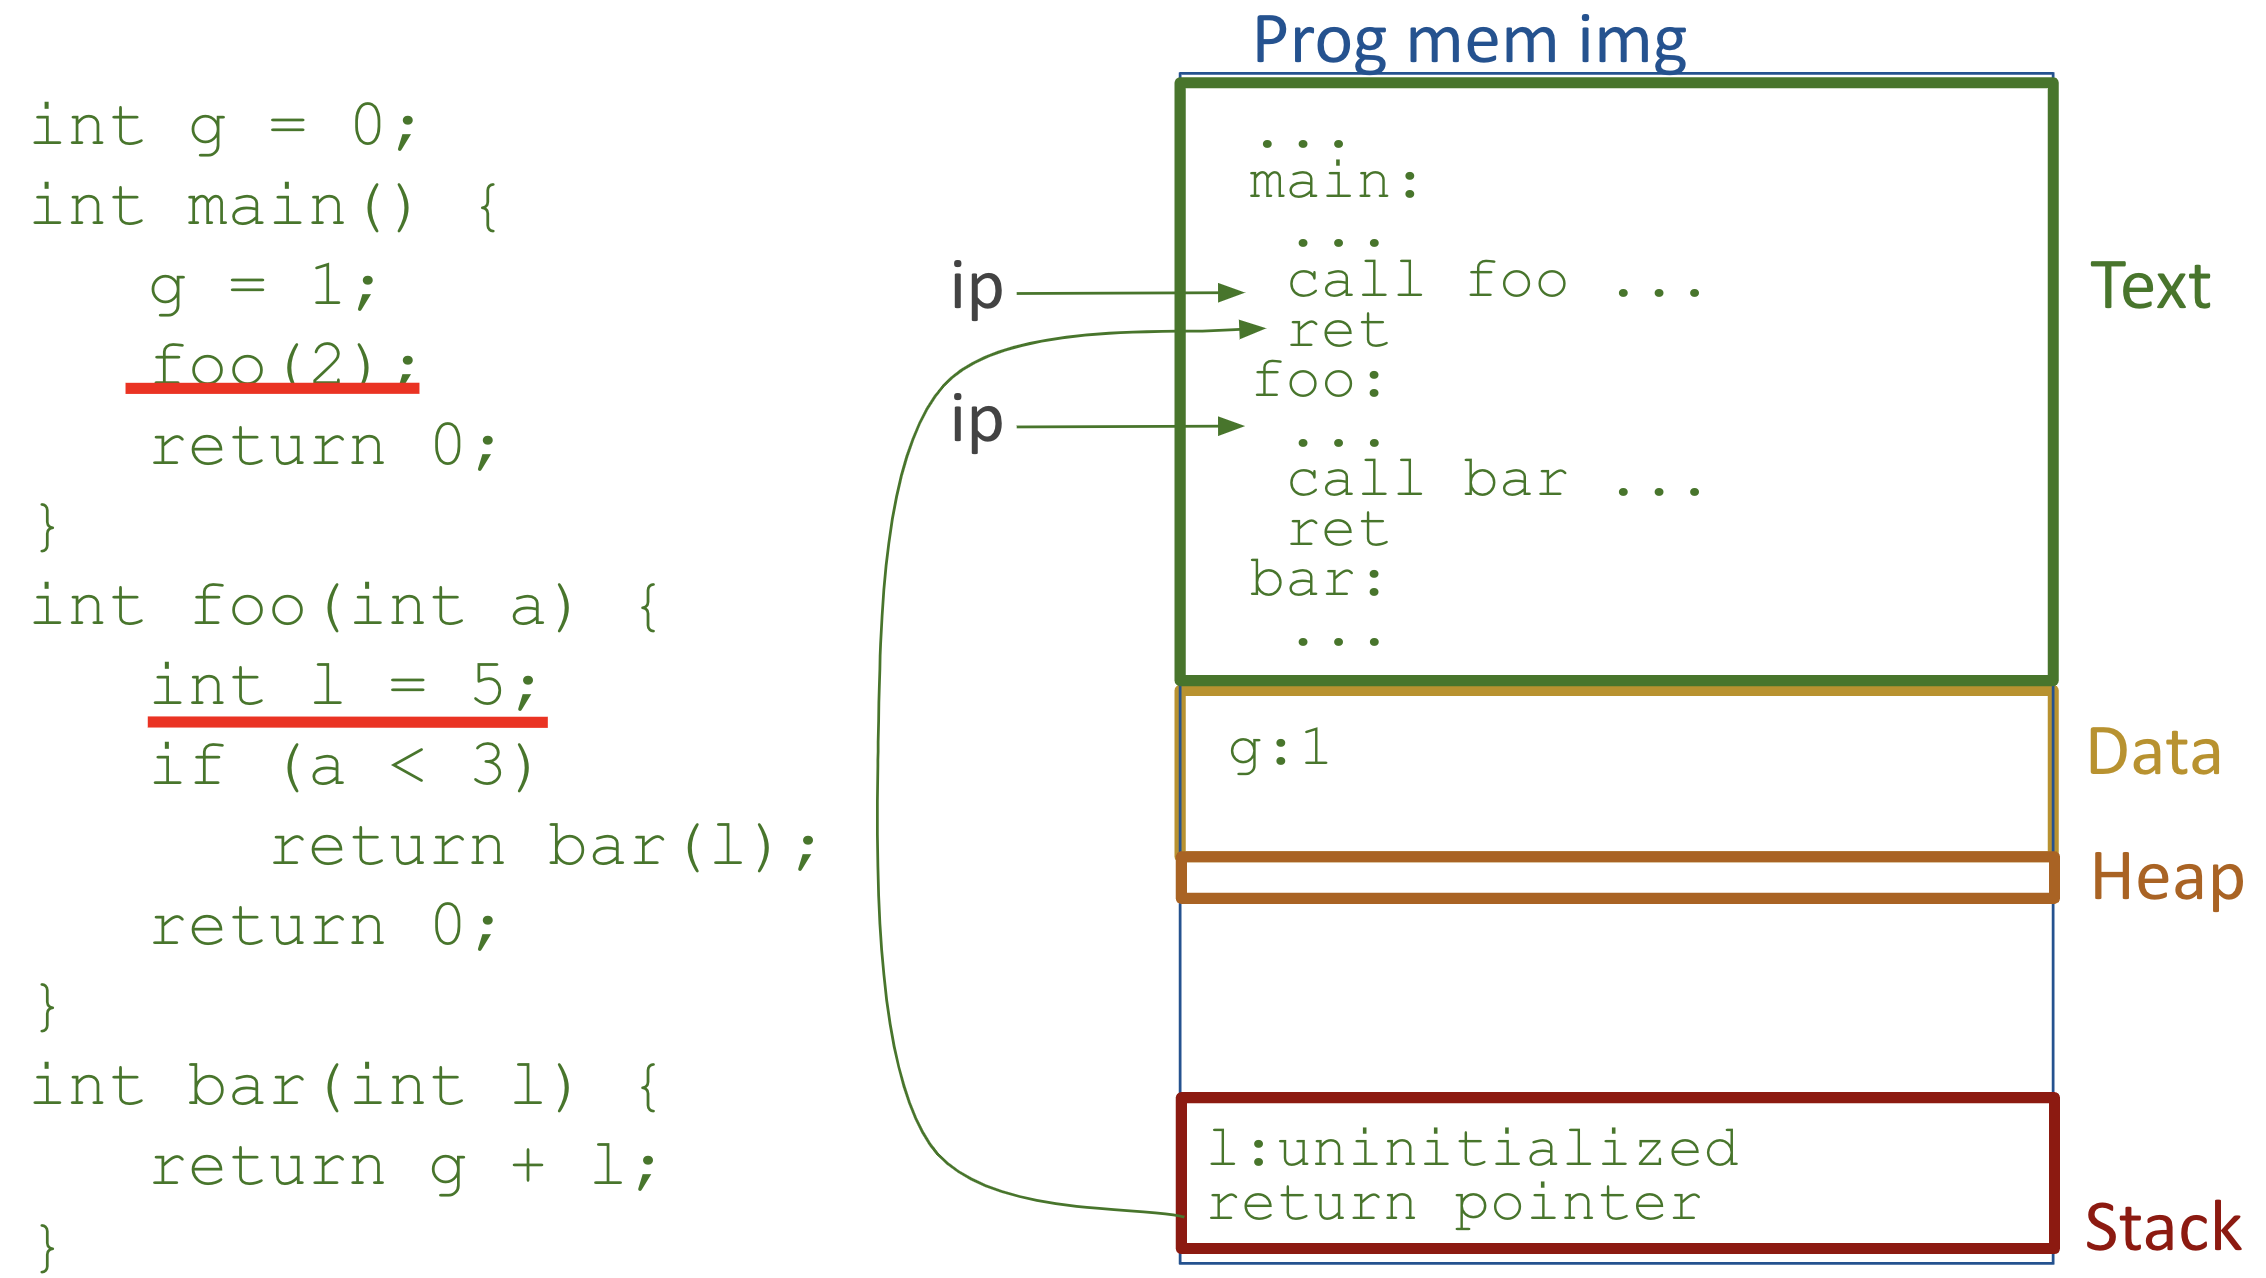
\includegraphics[width=1.23\textwidth]{chapters/L4/images/exam.png}
\end{center}
\end{minipage} \\[30px]

\textbf{Exam Question:} Show the memory image and indicate the moment when the stack reaches its maximum size.


For the program shown above, the expected result would be:
\begin{center}
  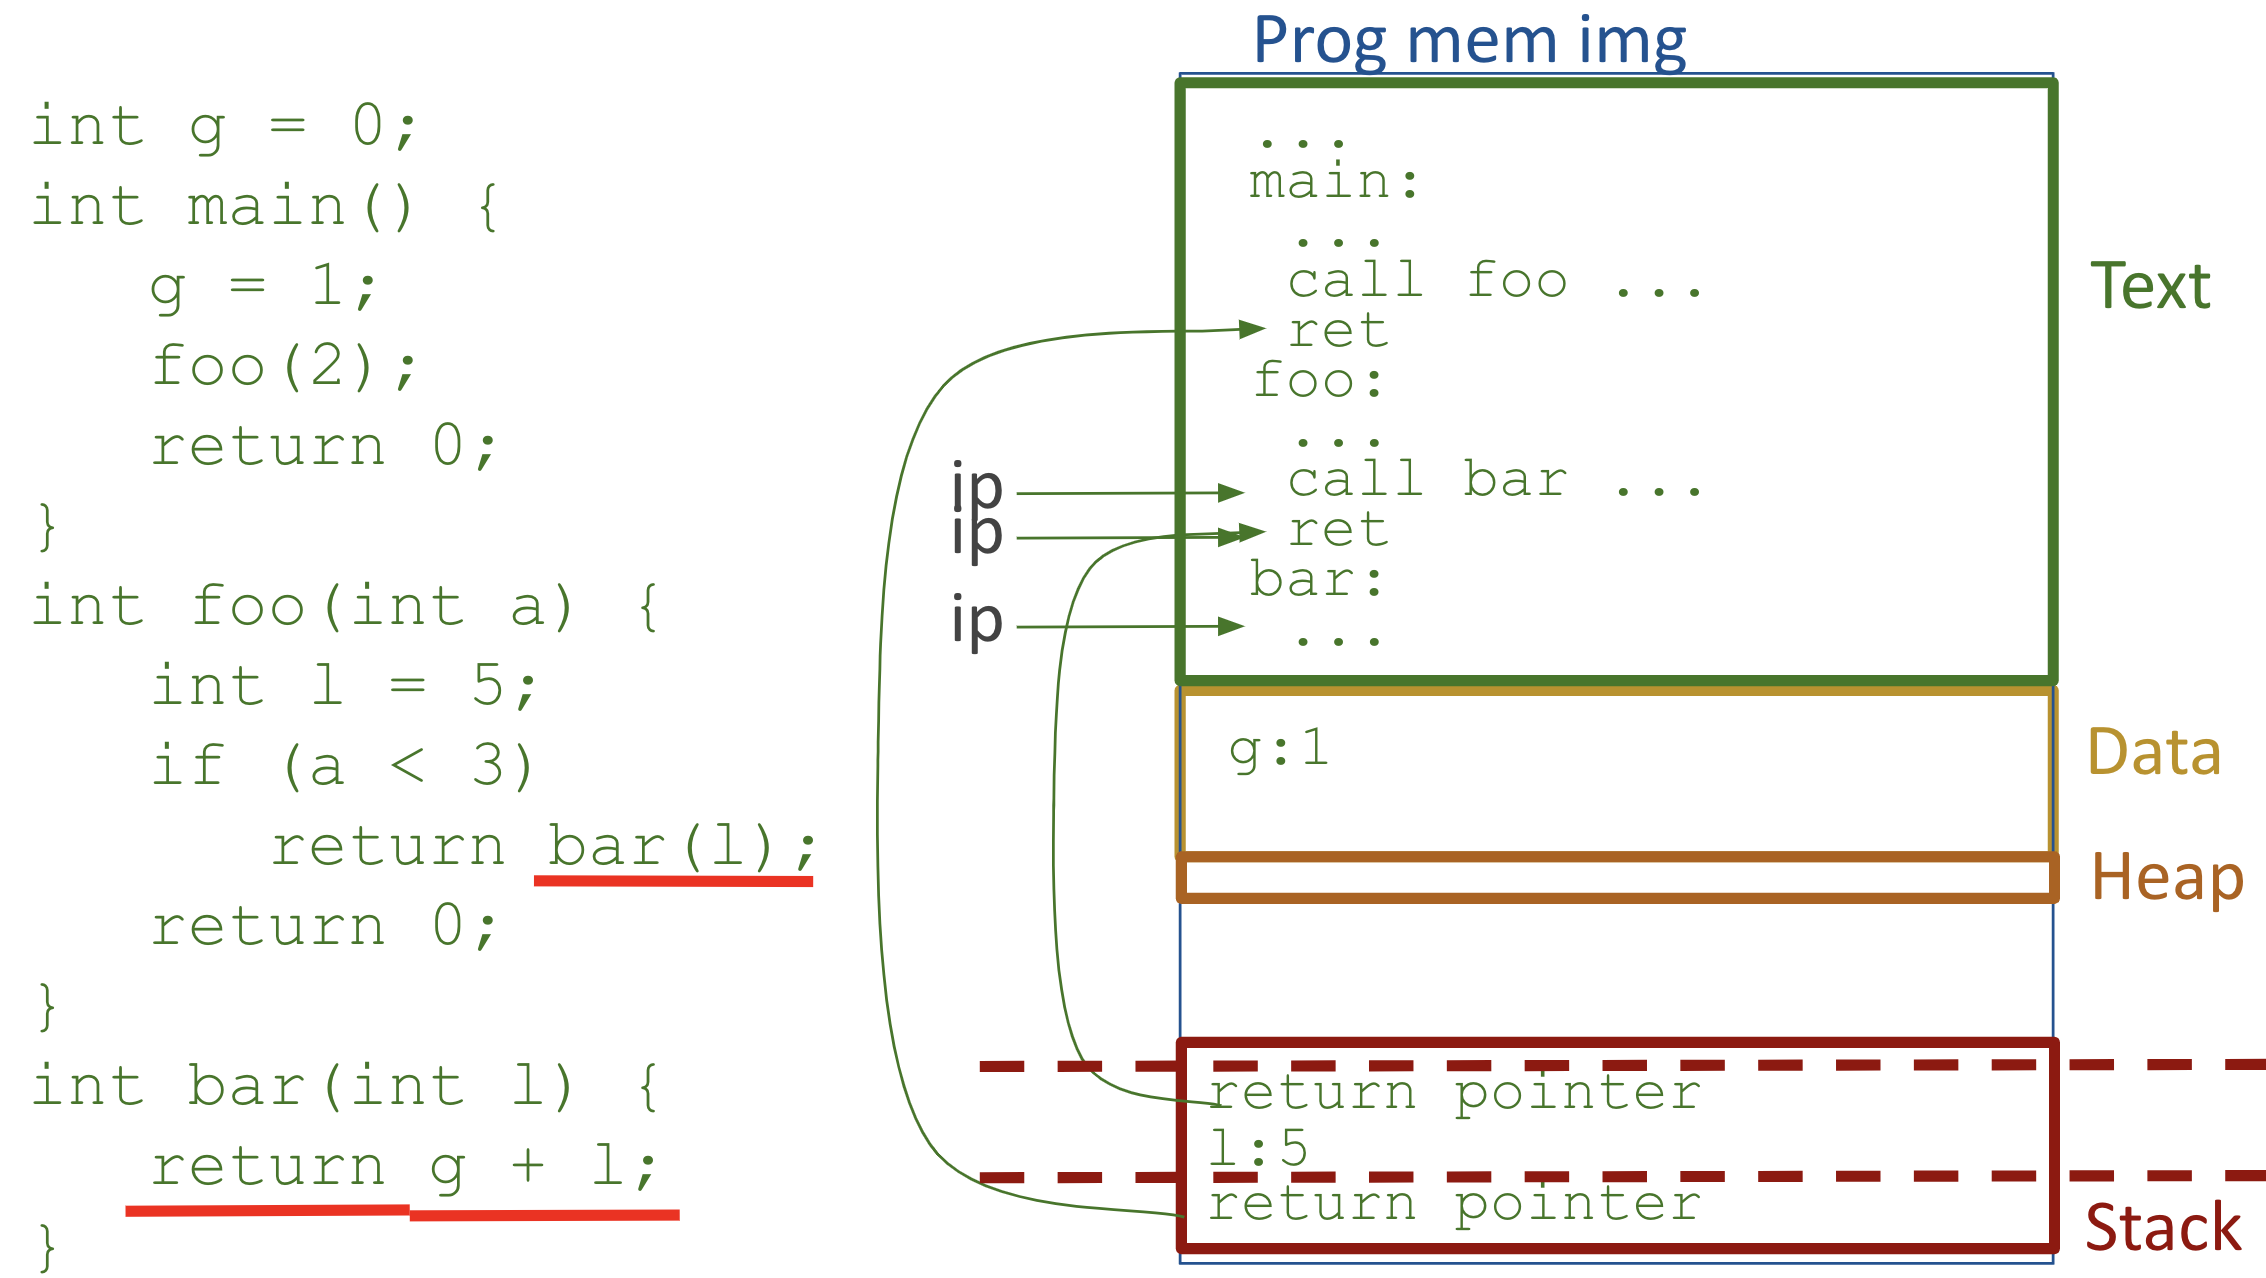
\includegraphics[width=0.65\textwidth]{chapters/L4/images/biggest-stack.png}
\end{center}

\newpage

\subsection{Optional - Stack and Register Functioning}

In modern computer architectures, the process of a function call involves a coordinated interplay between CPU registers and the stack.\\[8px]

\begin{definition}[Function Call Mechanism]
\leavevmode\\[5px]
During a function call:
\begin{enumerate}
    \item The \textbf{caller} passes arguments to the \textbf{callee} by storing values in designated CPU registers.
    \item The \textbf{callee} processes the call and returns a result by placing it in a specific register (for example, the \texttt{rax} register).
\end{enumerate}
\end{definition}

\begin{center}
    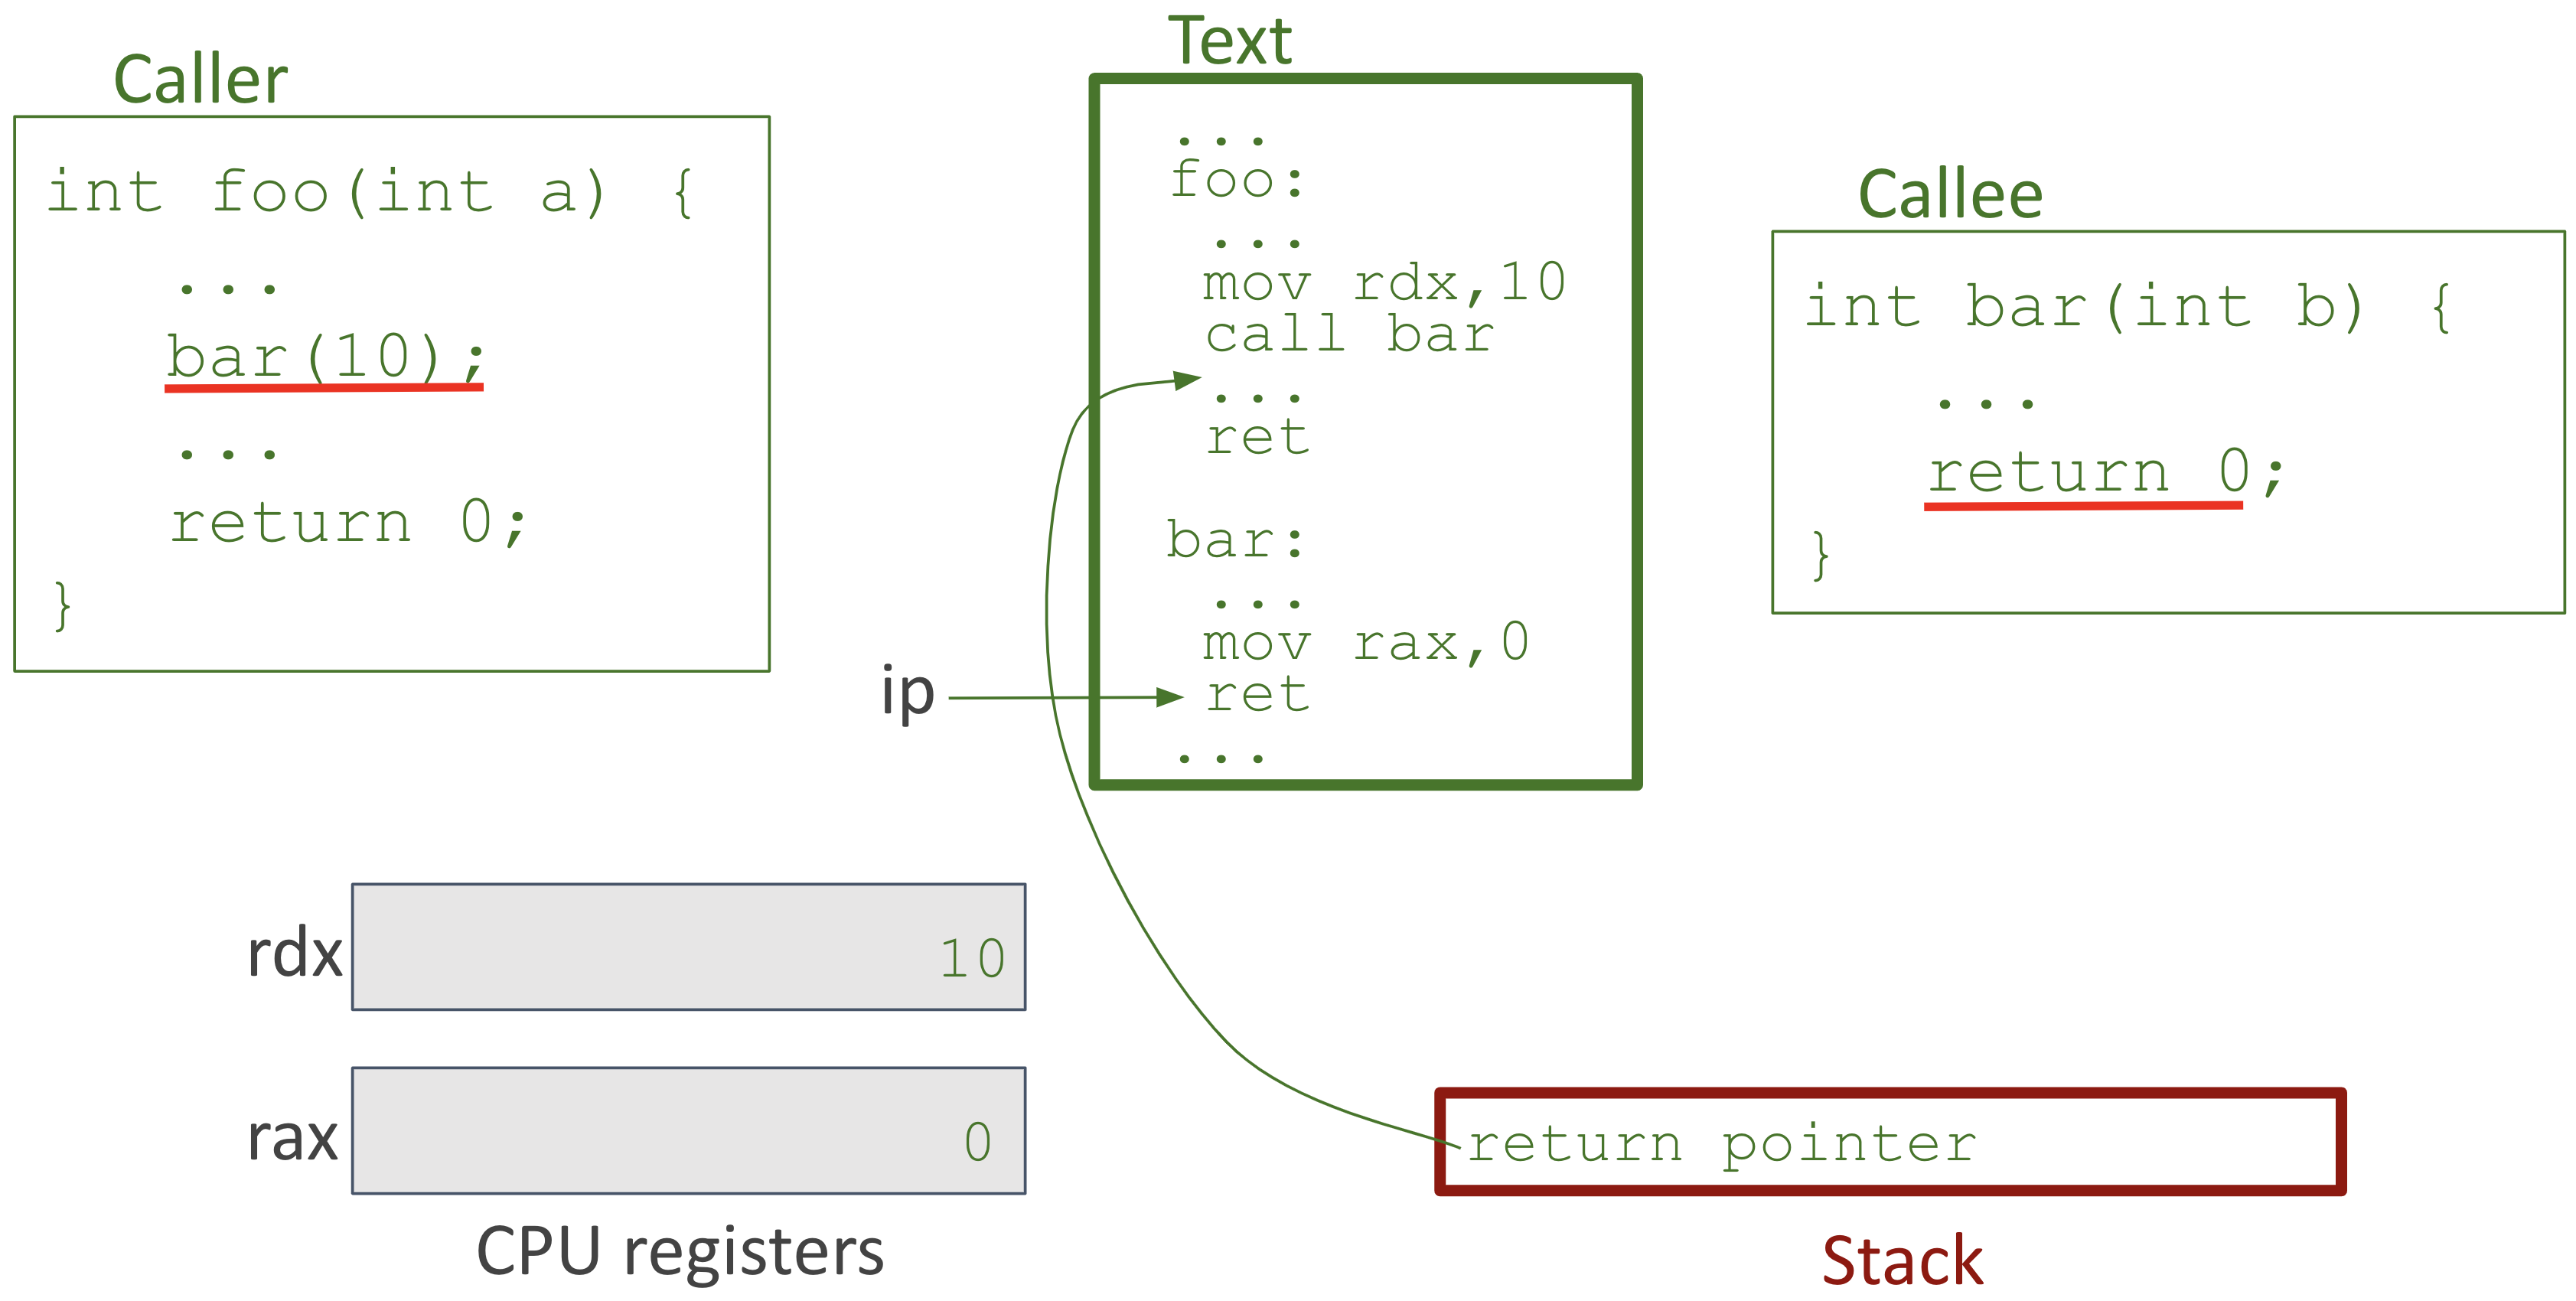
\includegraphics[width=0.65\textwidth]{chapters/L4/images/foo-bar.png}
\end{center}
\vspace{10px}
\begin{example}[Illustrative Function Call]
Consider the scenario where function \texttt{Foo} calls function \texttt{Bar}:
\begin{enumerate}
    \item \textbf{Argument Passing:} \texttt{Foo} stores the argument value (e.g., \textbf{10}) in a CPU register. 
    \item \textbf{Return Value Handling:} An implicit agreement between foo and bar that the return value will be stored in a particular register (eg. rax). \texttt{Bar} processes the argument and stores its return value in another register (e.g., \texttt{rax}). Later, \texttt{Foo} retrieves this value by accessing that register.
\end{enumerate}
\end{example}

A caller and a callee share common infrastructure by using CPU registers to maintain their context during the call. In addition, the stack is used to preserve register states when necessary:
\begin{itemize}
    \item \textbf{Caller-Saved Registers:} The caller saves certain registers to the stack before the call and restores them after the call returns.
    \item \textbf{Callee-Saved Registers:} The callee saves its registers at the beginning of the function and restores them before returning.
\end{itemize}
\textit{The stack, the register the calling conventions form a caller/callee interface.}\\
Adhering to these calling conventions is critical; for instance, if the callee writes into the caller's stack frame, it may lead to stack smashing and compromise program stability.



\newpage
\section{Memory Virtualization}
In modern operating systems, each process references memory using virtual addresses. Underneath, these virtual addresses are translated to physical addresses. Importantly, each process has its own virtual address space, which means that two processes may use the same virtual address while referring to entirely different physical locations. This design creates the \textbf{safe illusion} that main memory “belongs” exclusively to each process, greatly simplifying program development and enhancing security.

\noindent
\begin{minipage}{0.45\textwidth}
Each address in the image refers to an address within its own stack. The addresses shown are \emph{virtual}, meaning they are process-specific (e.g., address 0 in one process does not necessarily correspond to address 0 in another).
\end{minipage}%
\hfill
\vline
\hfill
\begin{minipage}{0.45\textwidth}
\begin{center}
    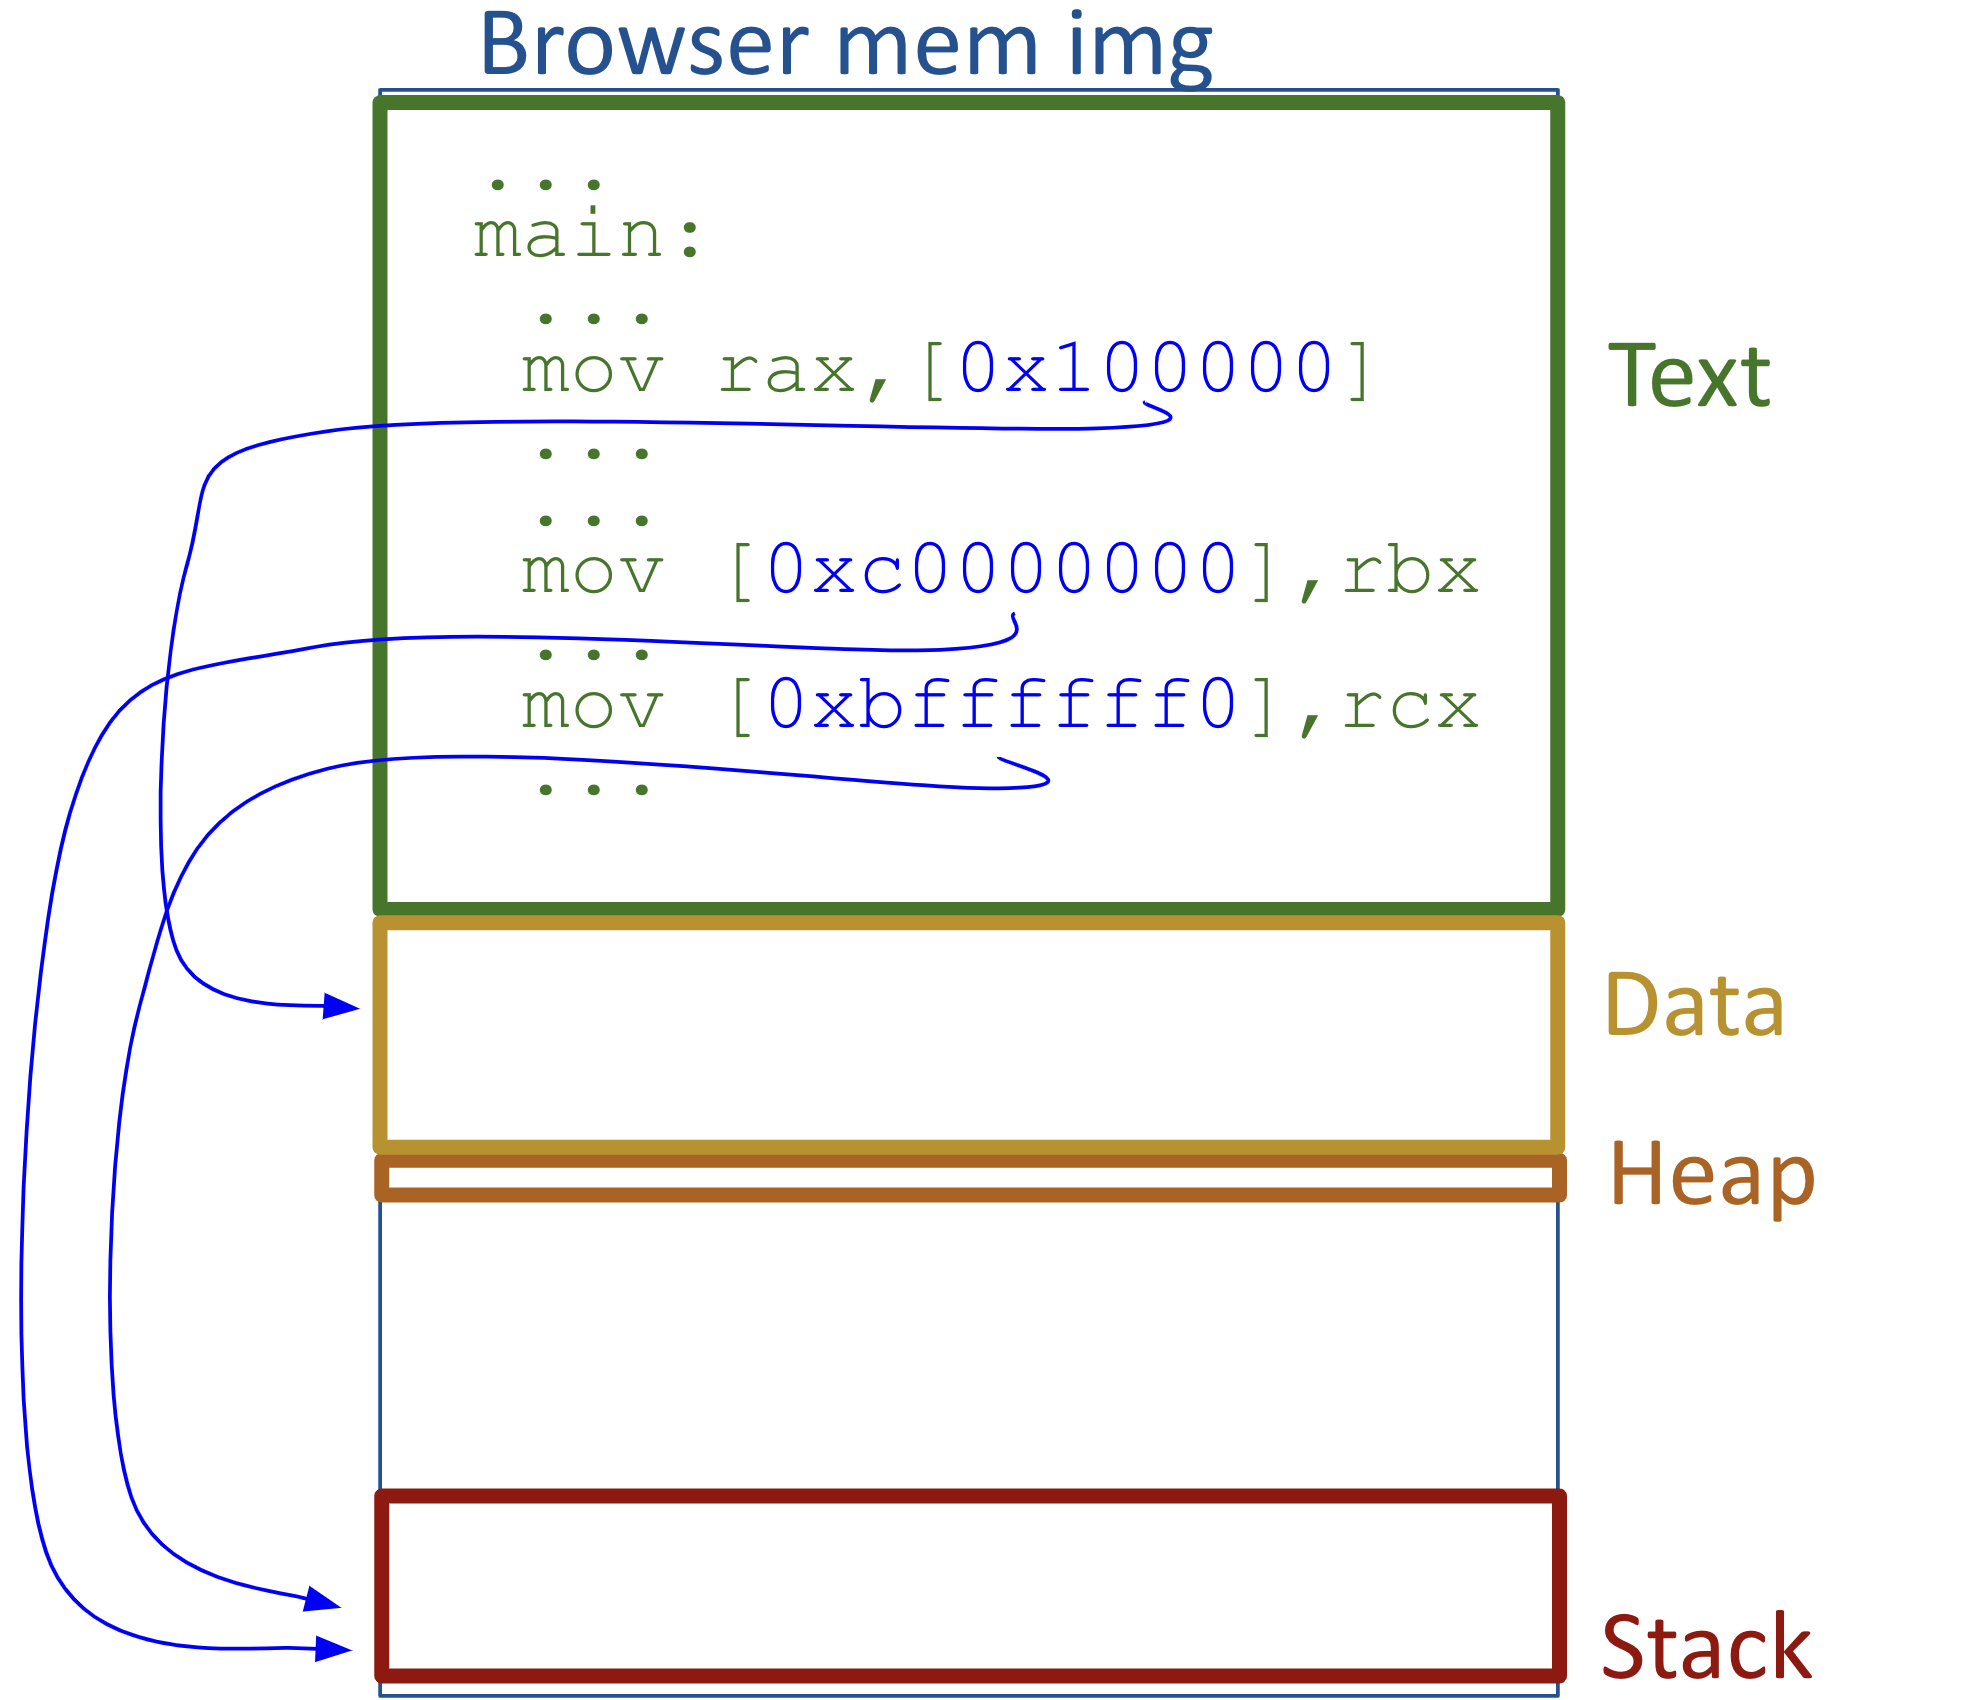
\includegraphics[width=0.85\textwidth]{chapters/L4/images/browser-img.png}
\end{center}
\end{minipage}\\[10px]

\noindent
\begin{minipage}{0.45\textwidth}
\textbf{Exam Question:} If two memory instructions read the same virtual address, is it the same physical address? \\[3px]
\textbf{Answer:} Yes, when they are translated to the same physical memory address, as they belong to the same virtual address space.
\end{minipage}%
\hfill
\vline
\hfill
\begin{minipage}{0.45\textwidth}
\begin{center}
    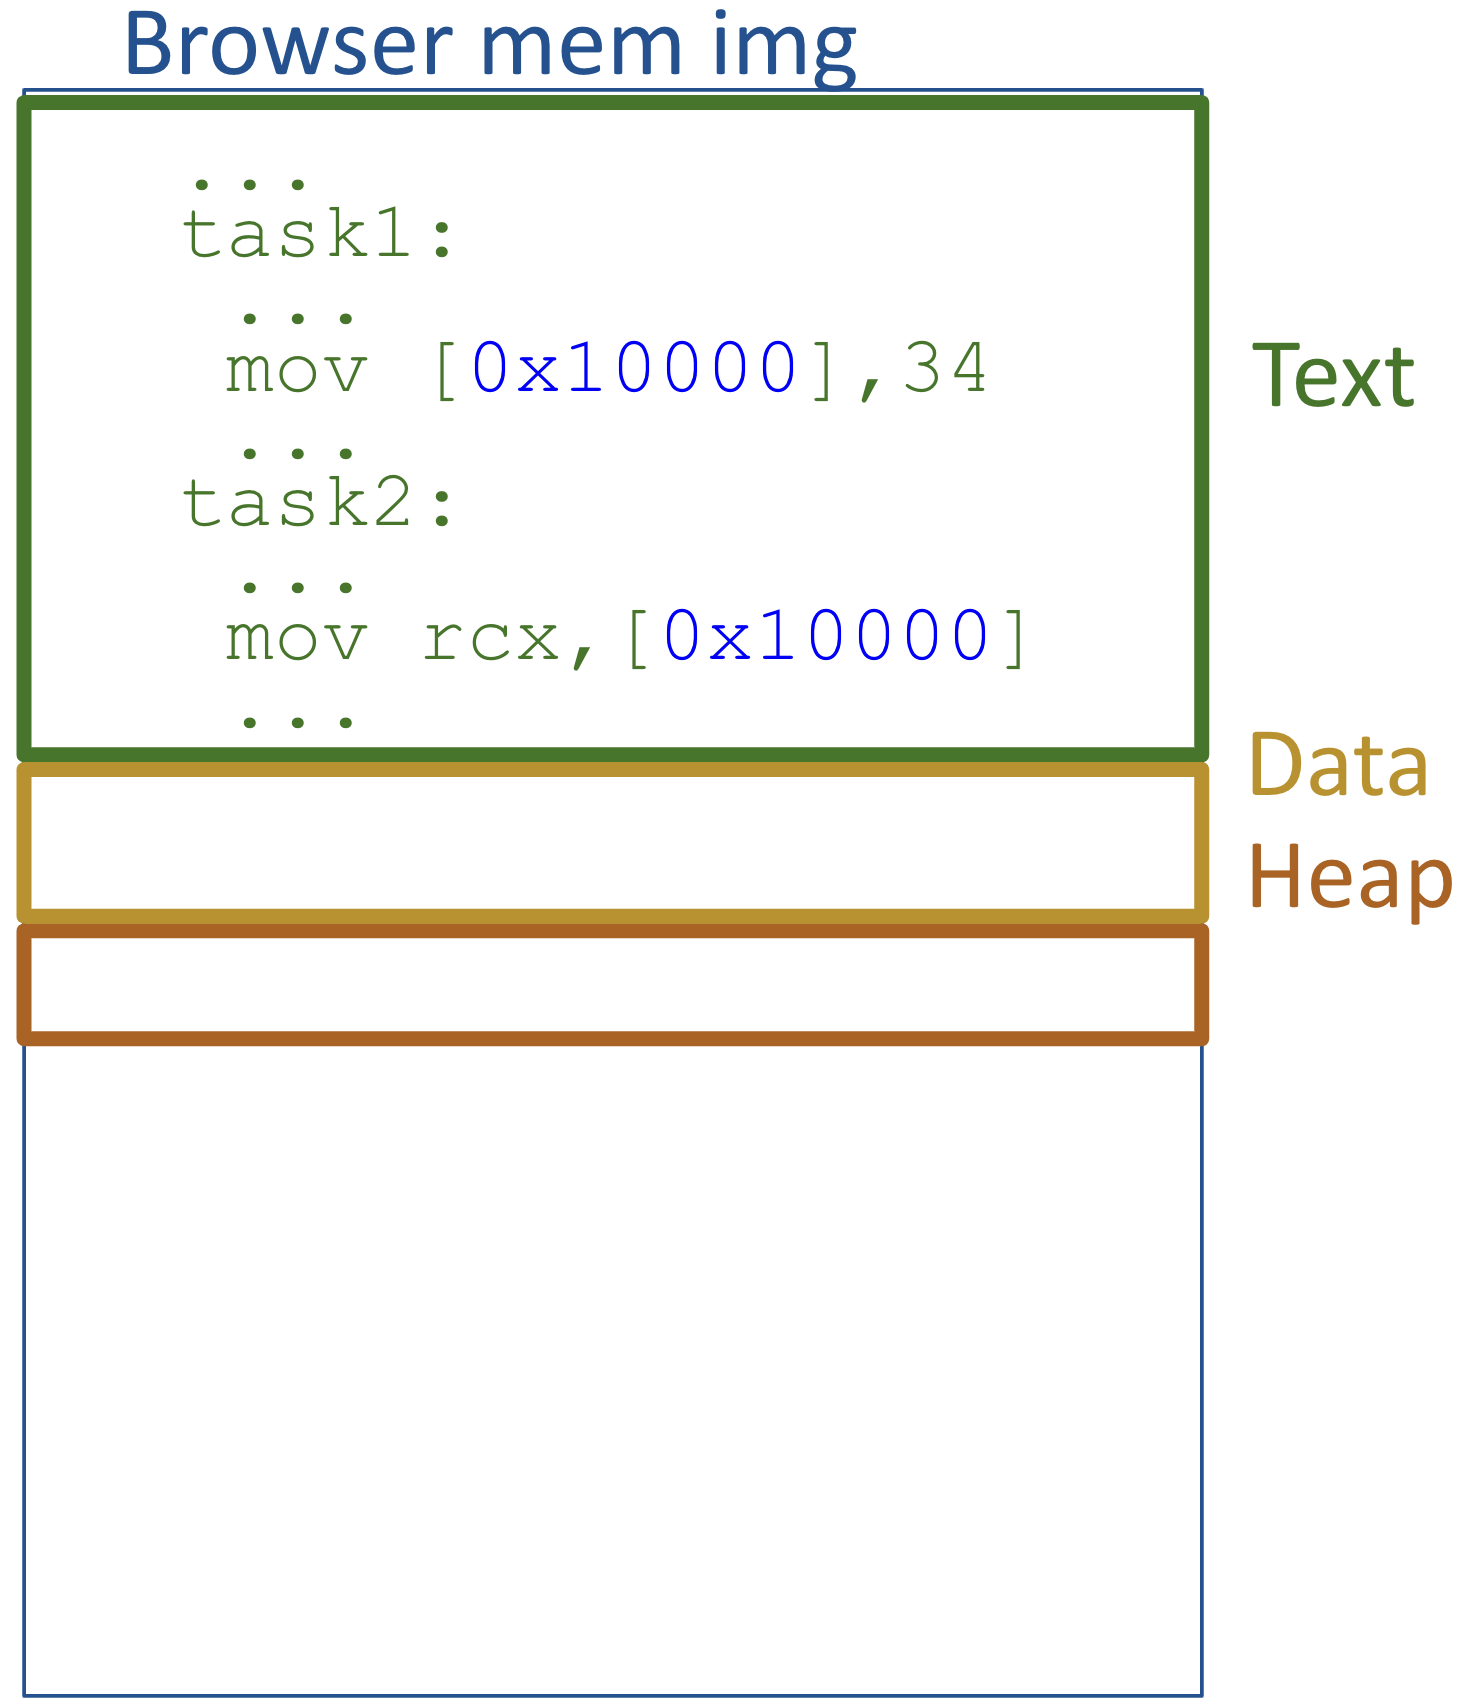
\includegraphics[width=0.7\textwidth]{chapters/L4/images/two-proc.png}
\end{center}
\end{minipage}
\\[10px]

\noindent
\begin{minipage}{0.45\textwidth}
\textbf{Exam Question:} Are these two processes accessing the same memory location? \\[3px]
\textbf{Answer:} No, they are not actually accessing the same physical memory. Although both use the address 0x10000, each process runs in its own virtual address space. 
\end{minipage}%
\hfill
\vline
\hfill
\begin{minipage}{0.45\textwidth}
\begin{center}
    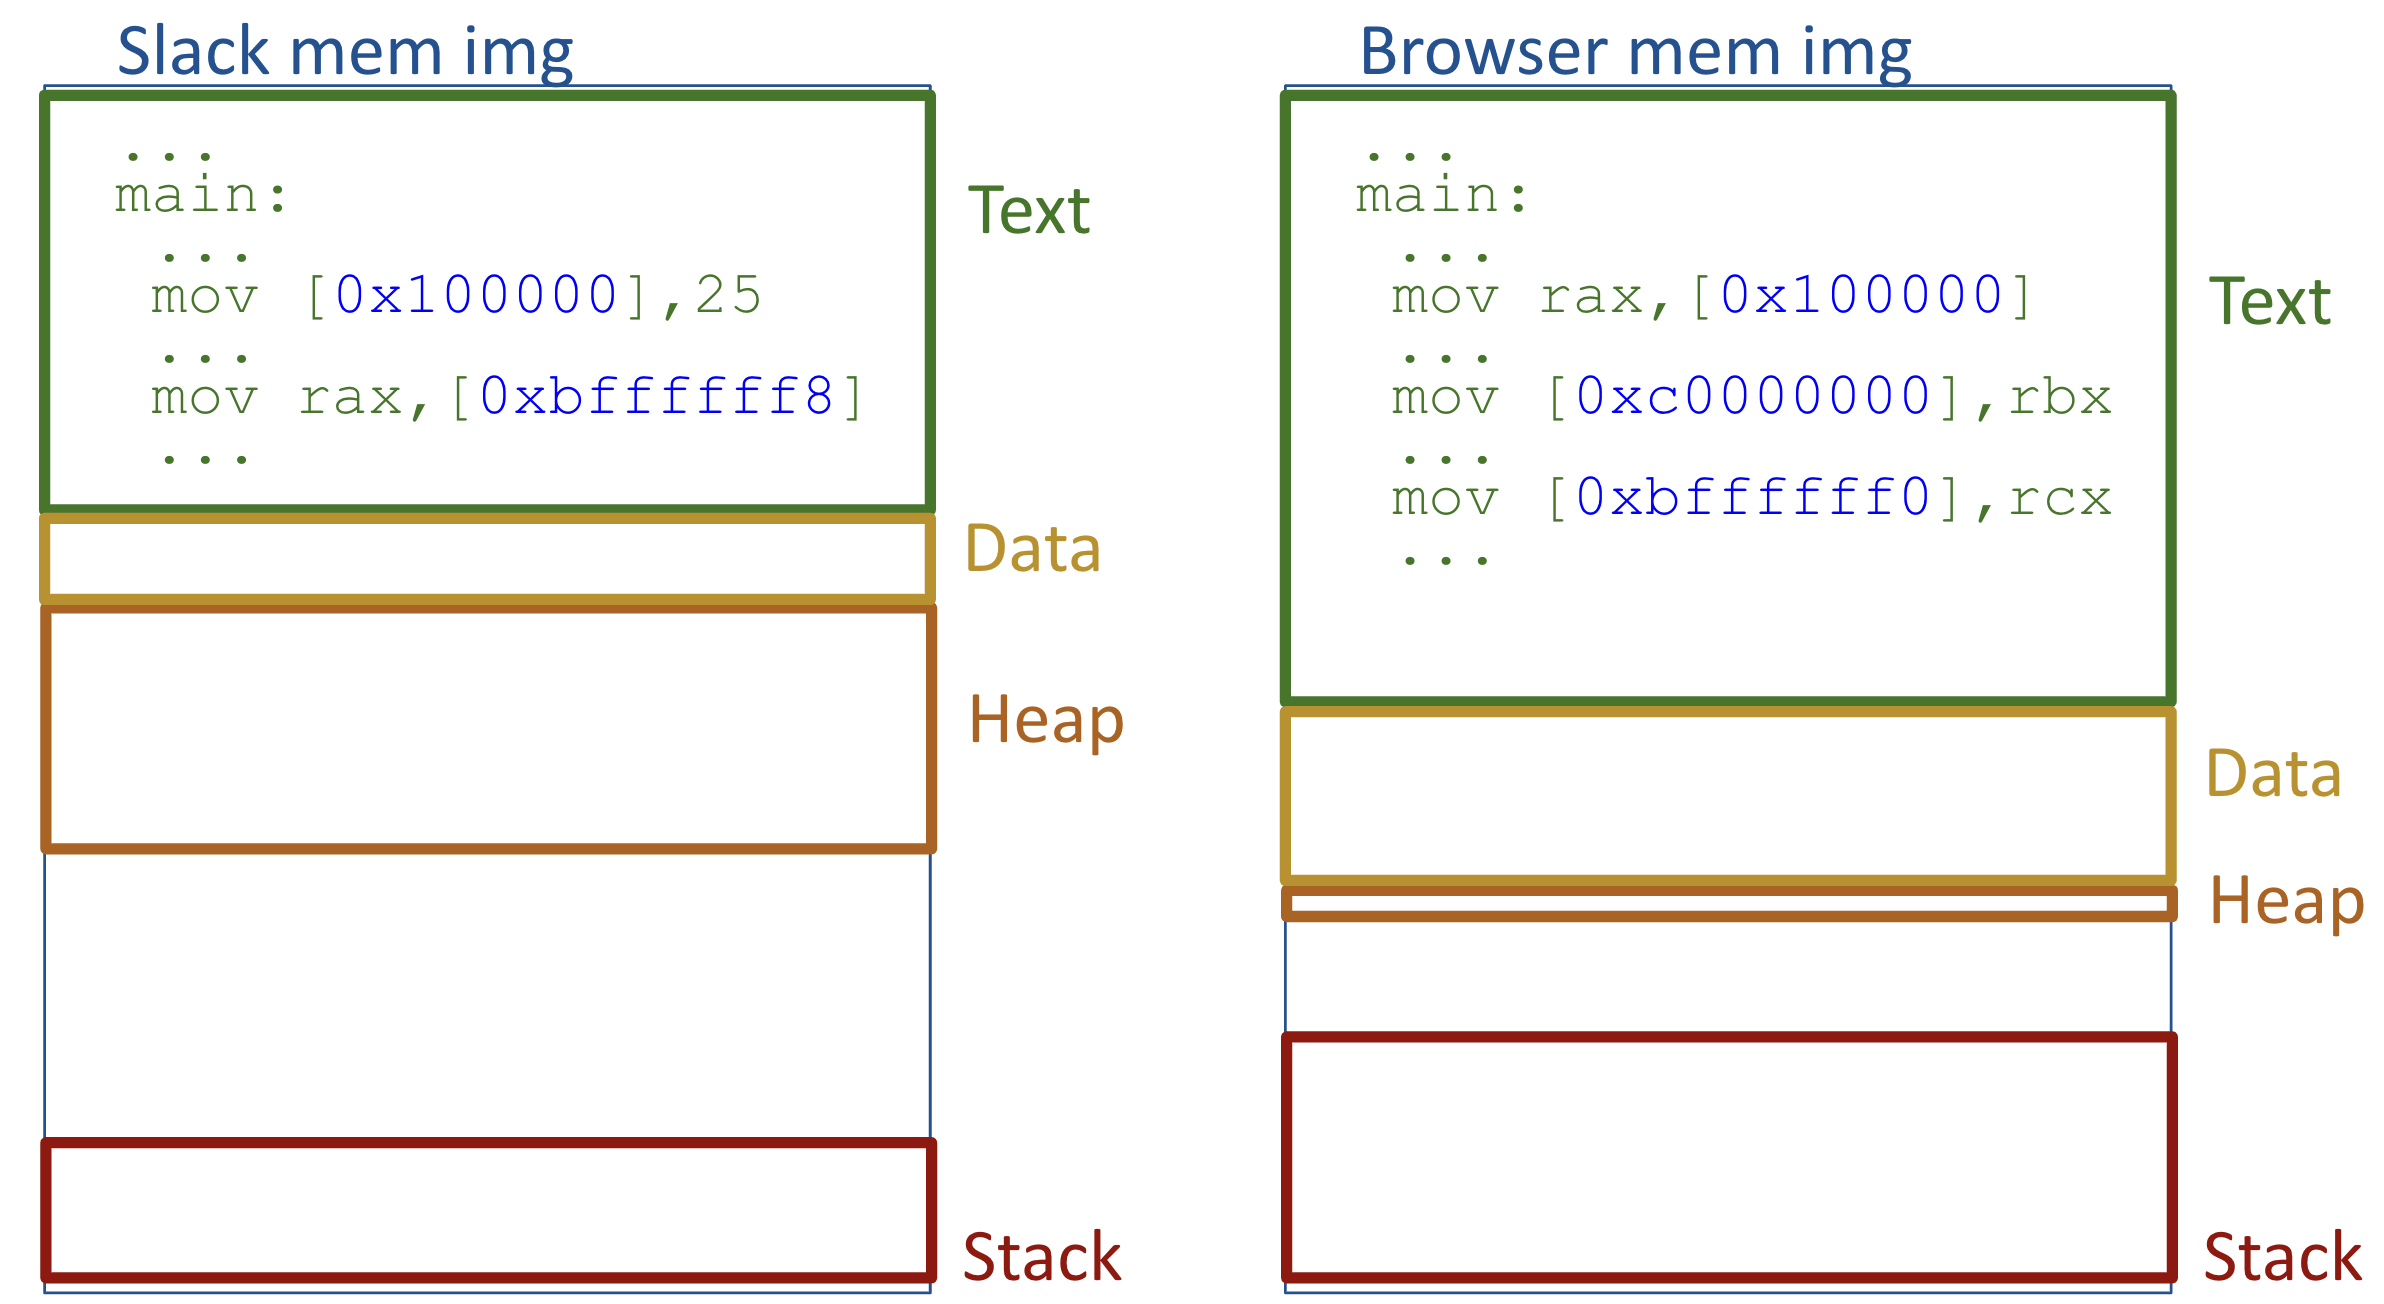
\includegraphics[width=1.25\textwidth]{chapters/L4/images/virtual.png}
\end{center}
\end{minipage}\\[14px]

The mechanism of memory virtualization creates a \emph{safe illusion} in which it appears that the main memory is exclusively owned by each process. This design not only simplifies the generation of executable programs but also enforces security by ensuring that a process can only access its own memory image.

\begin{definition}[Contiguous Memory]
\leavevmode\\[2px]
Contiguous memory refers to a block of physical memory addresses that are sequentially arranged. In this allocation scheme, the entire memory image of a process is stored in one unbroken segment, simplifying the translation from virtual to physical addresses.
\end{definition}

\subsection{Memory Management Unit --- Simple Implementation}
\vspace{10px}
\noindent The \textbf{Memory Management Unit (MMU)} is a specialized piece of \textit{hardware} that translates virtual memory addresses into physical addresses.\\[10px]
\vspace{10px}
\noindent
\begin{minipage}{0.45\textwidth}
  For each process, the \textbf{OS kernel} sets up \emph{base} and \emph{bound} registers (which are physically stored in the CPU). The MMU then uses these values to ensure that the process’s memory image is allocated in a contiguous block of physical memory.\\[10px]
\begin{center}
  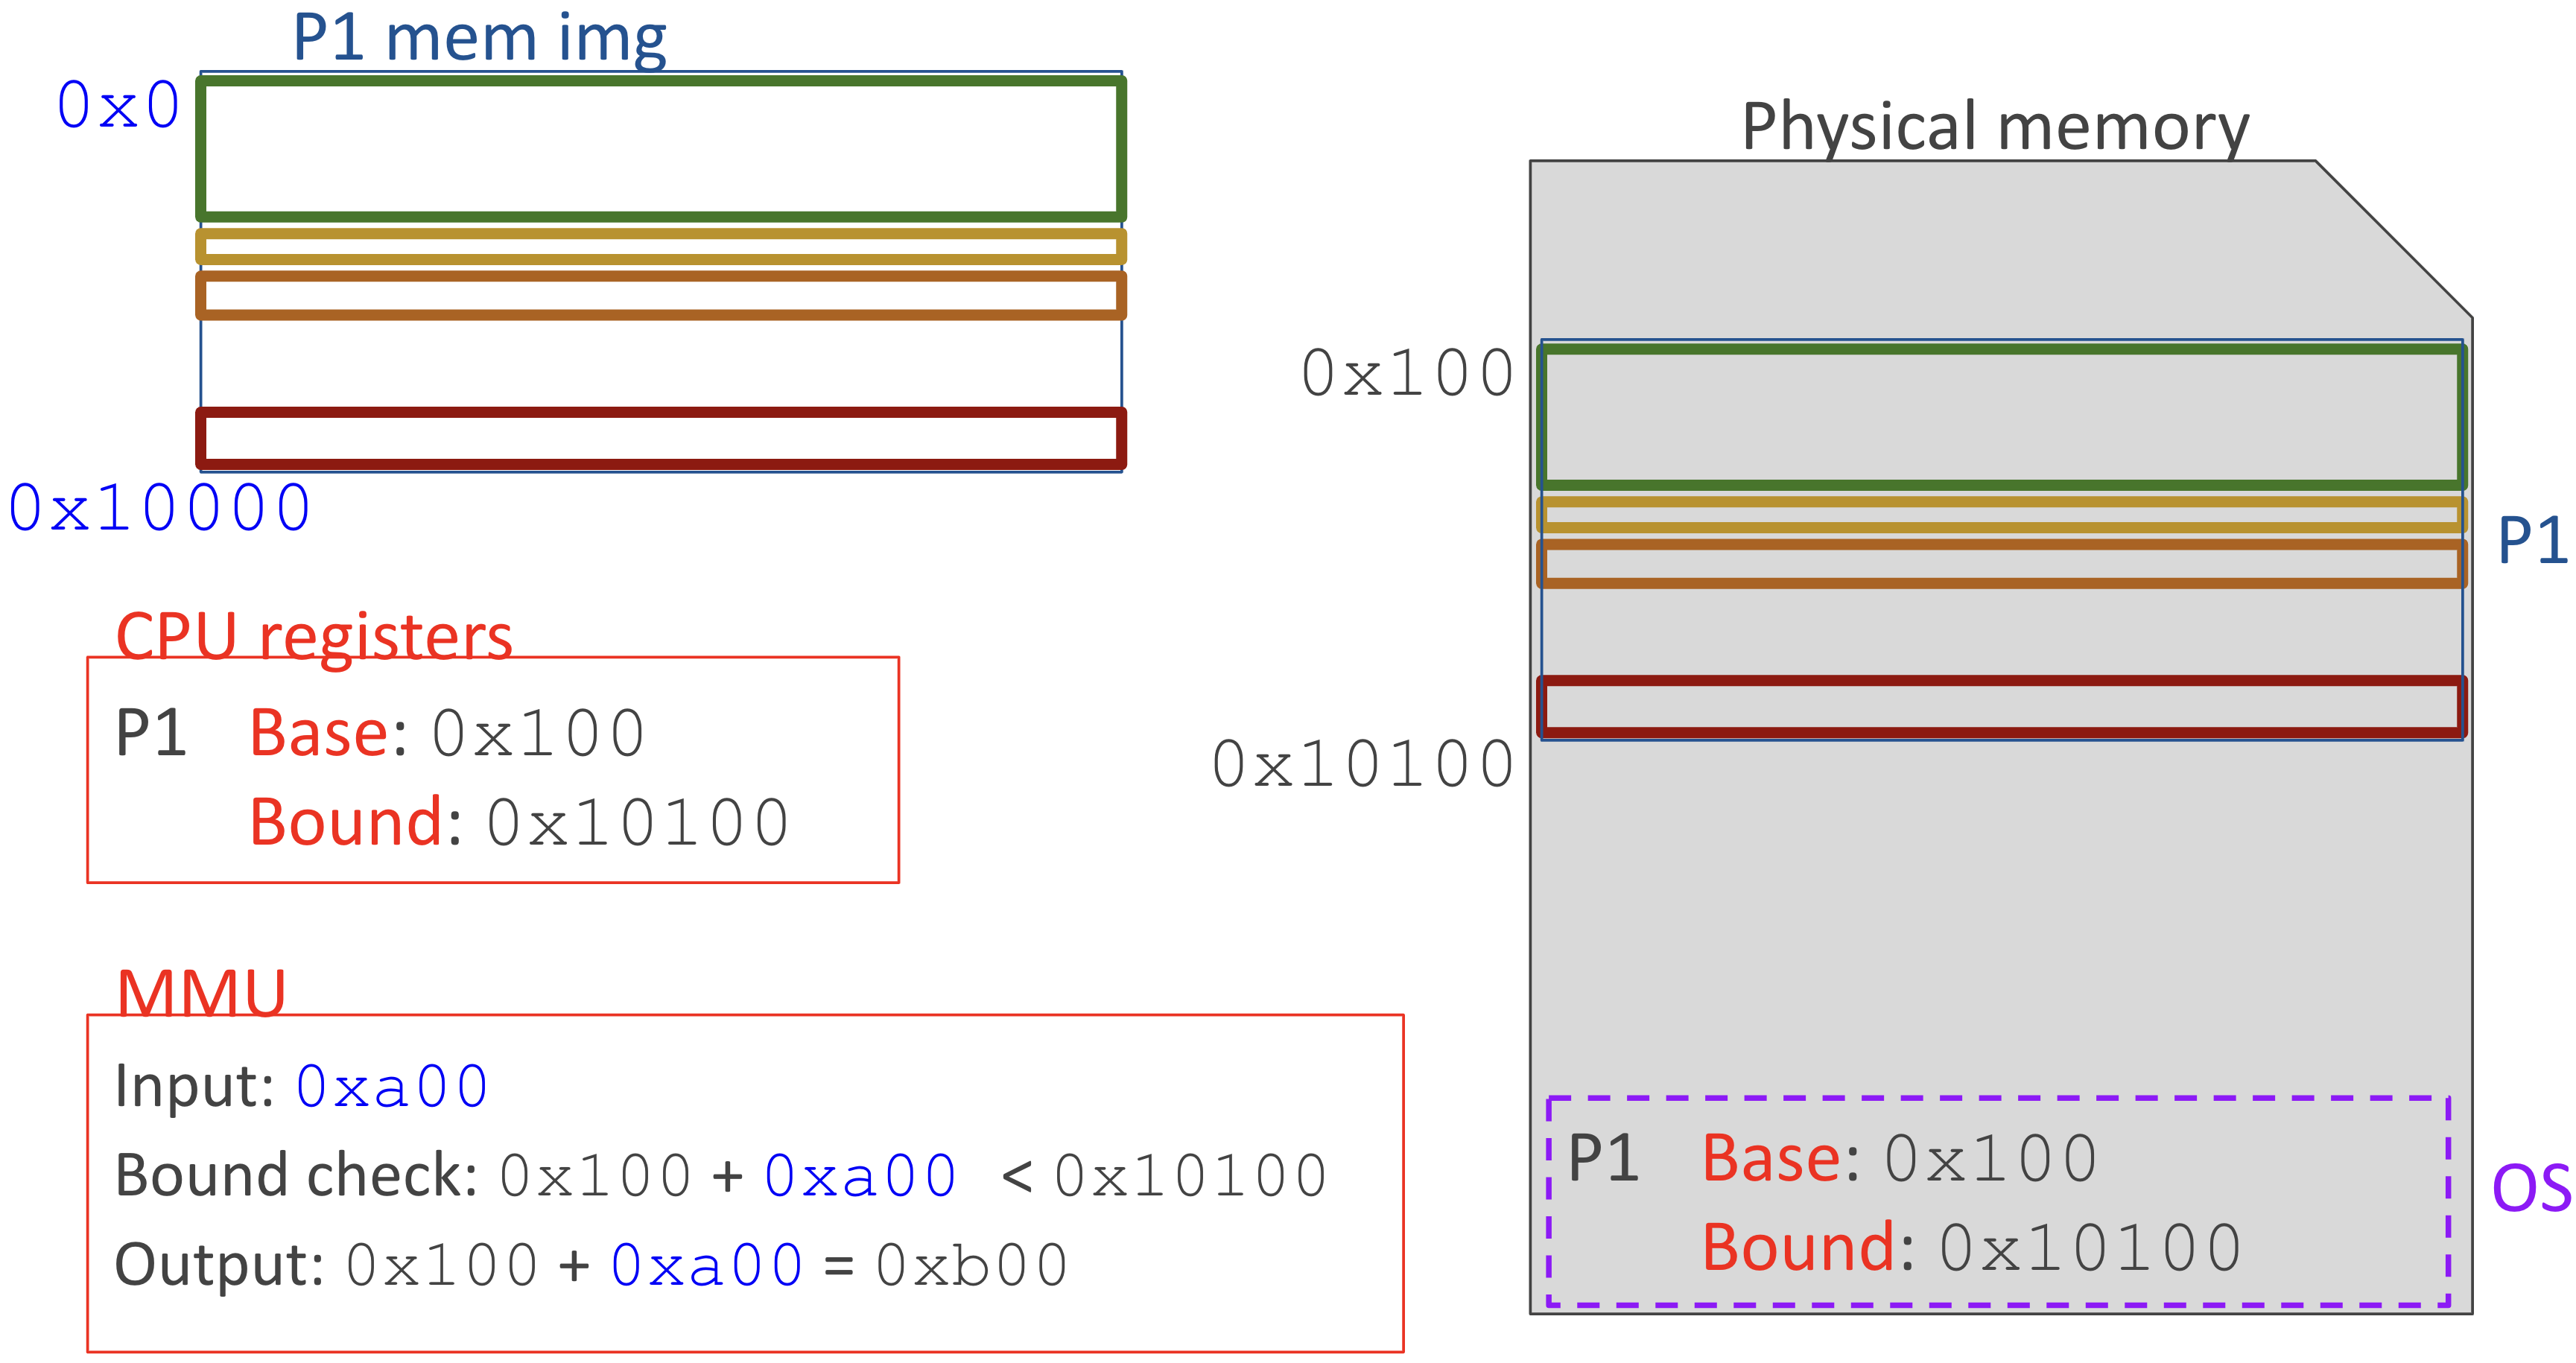
\includegraphics[width=1.1\textwidth]{chapters/L4/images/indirection.png}
\end{center}
\end{minipage}%
\hfill
\vline
\hfill
\begin{minipage}{0.45\textwidth}
\noindent When a second process (\(P_2\)) is introduced, the MMU checks its corresponding base and bound registers to determine the physical memory range in which \(P_2\) should be placed.
\begin{center}
  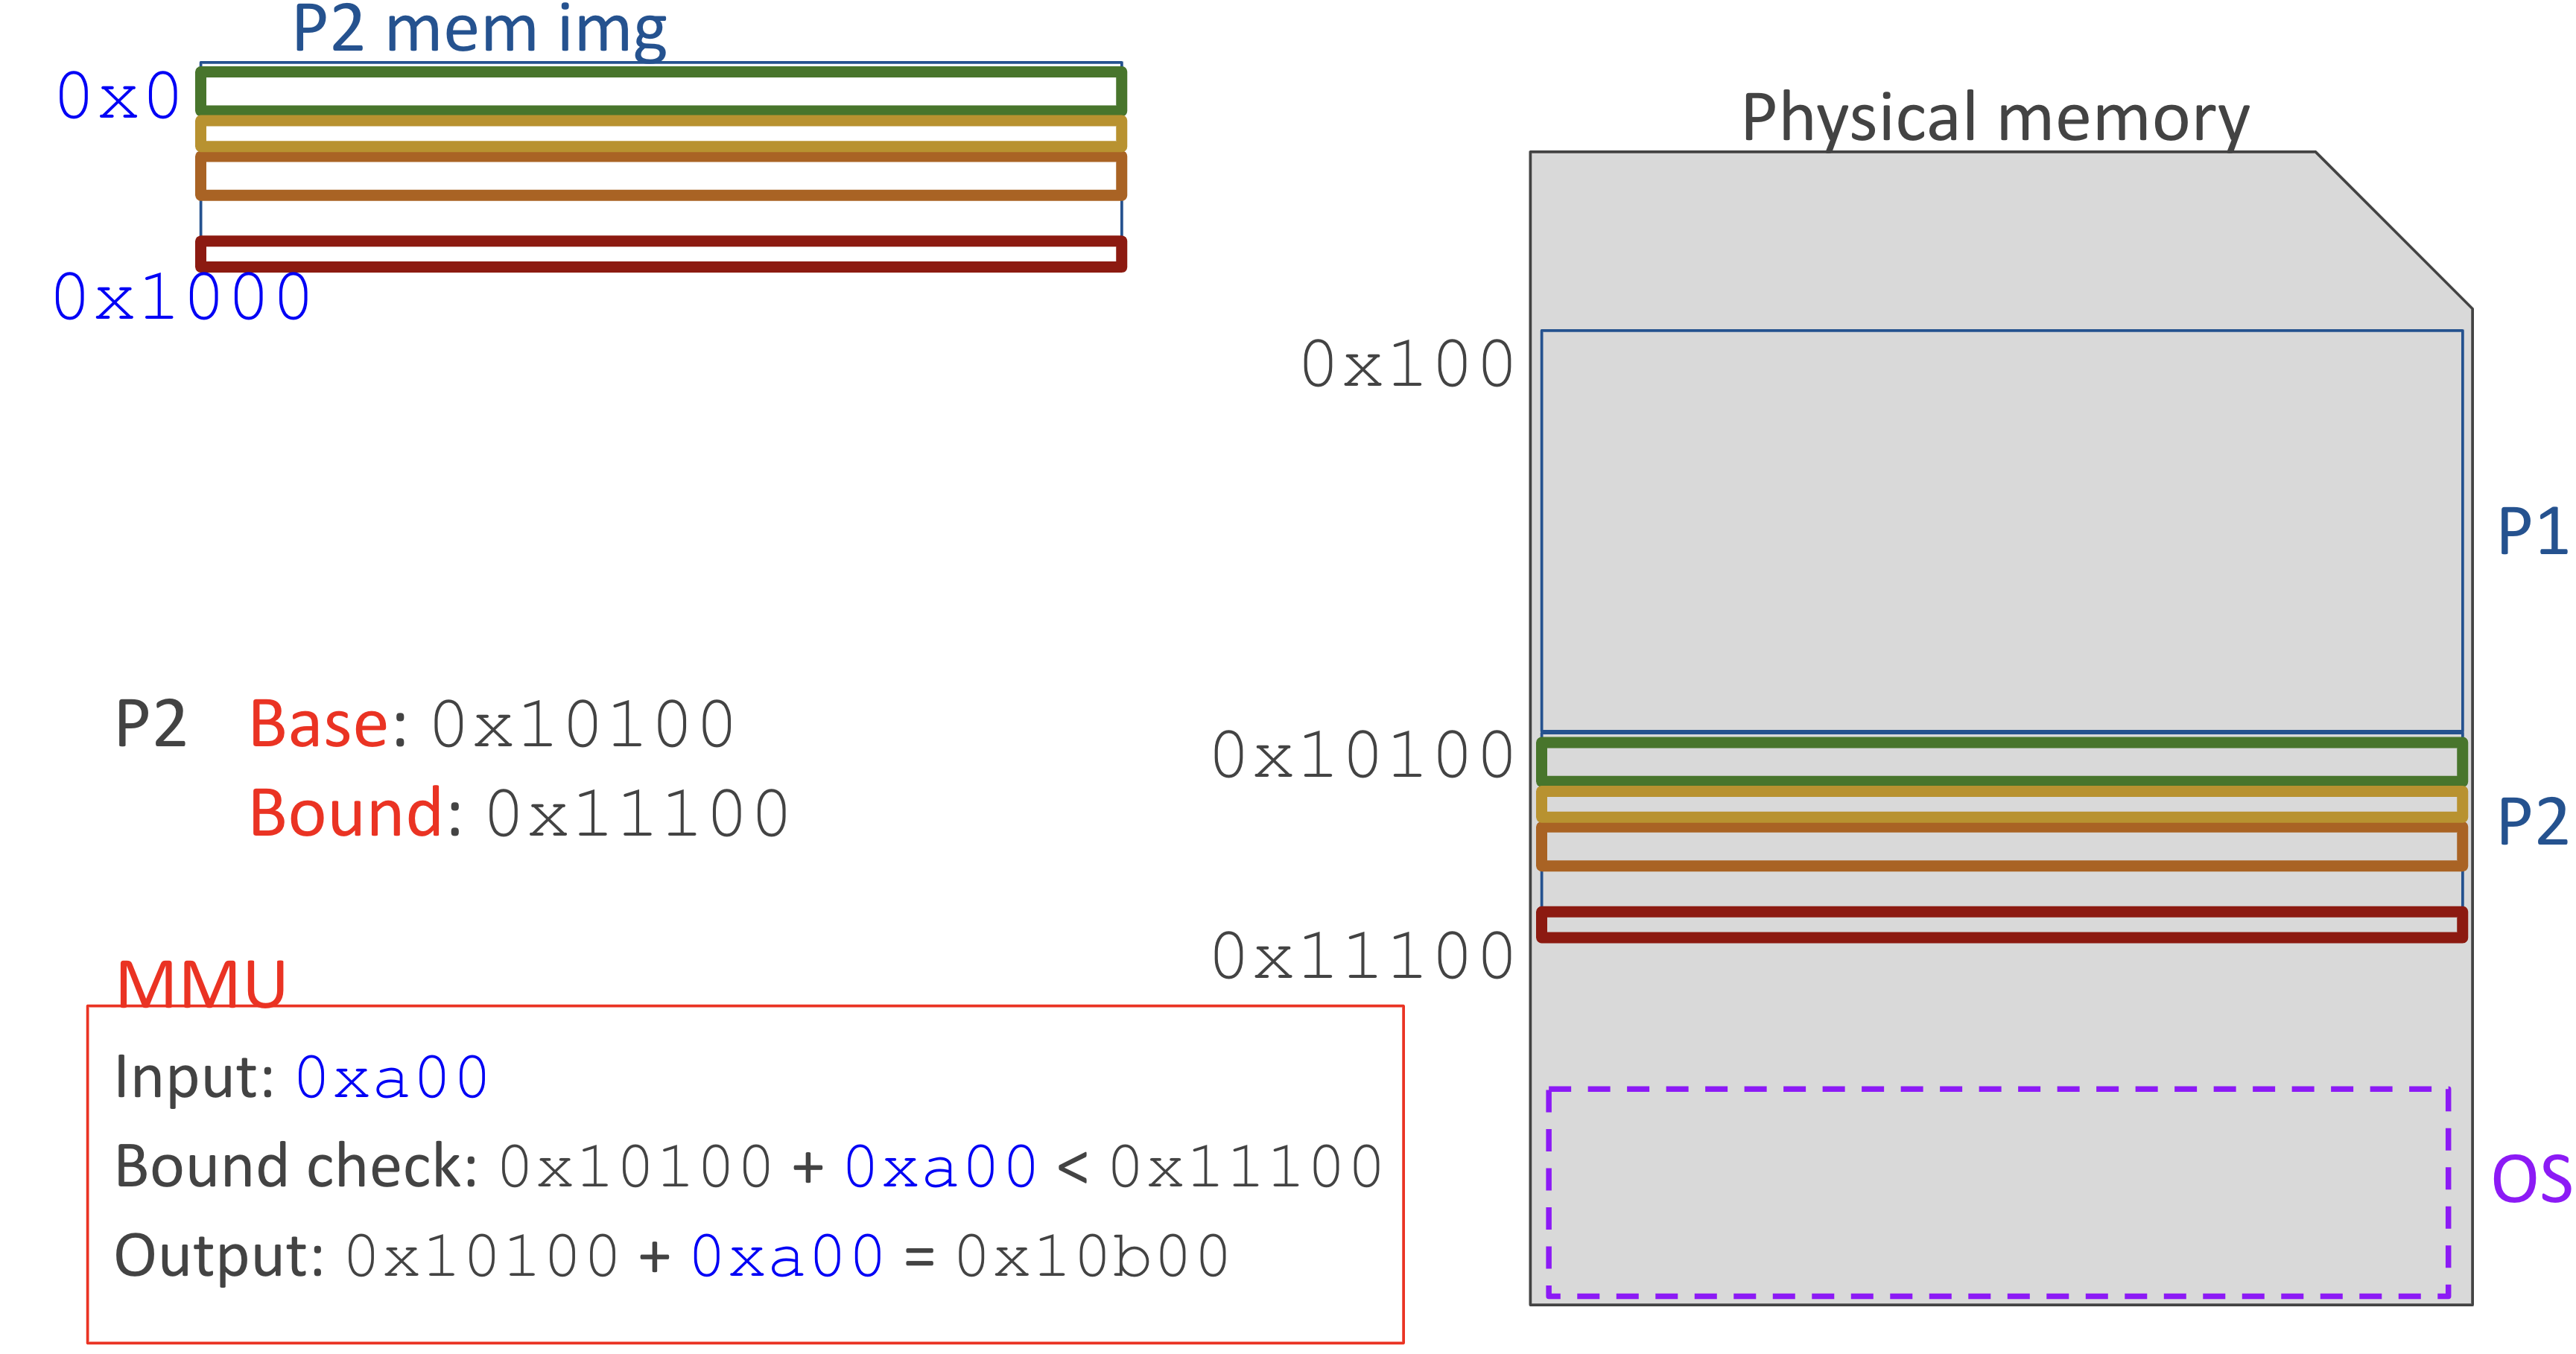
\includegraphics[width=1.1\textwidth]{chapters/L4/images/indirection-P2.png}
\end{center}
\end{minipage}
\\[70px]

\noindent In this \textbf{base--bound} scheme, each process’s memory image starts at its base address and extends just before its bound address. This approach is \textit{safe} (preventing a process from accessing memory outside its allocation) and preserves the \textit{illusion} of owning the entire memory. \\[3px]

However, because each process must reside in one contiguous memory block, \textbf{fragmentation} can occur. \\[15px]
\noindent
\begin{minipage}{0.45\textwidth}
For example, when process \(P_1\) terminates, it might leave a gap that is too small for a new process \(P_3\), even if the total available memory is sufficient.
\end{minipage}%
\hfill
\vline
\hfill
\begin{minipage}{0.45\textwidth}
\begin{center}
  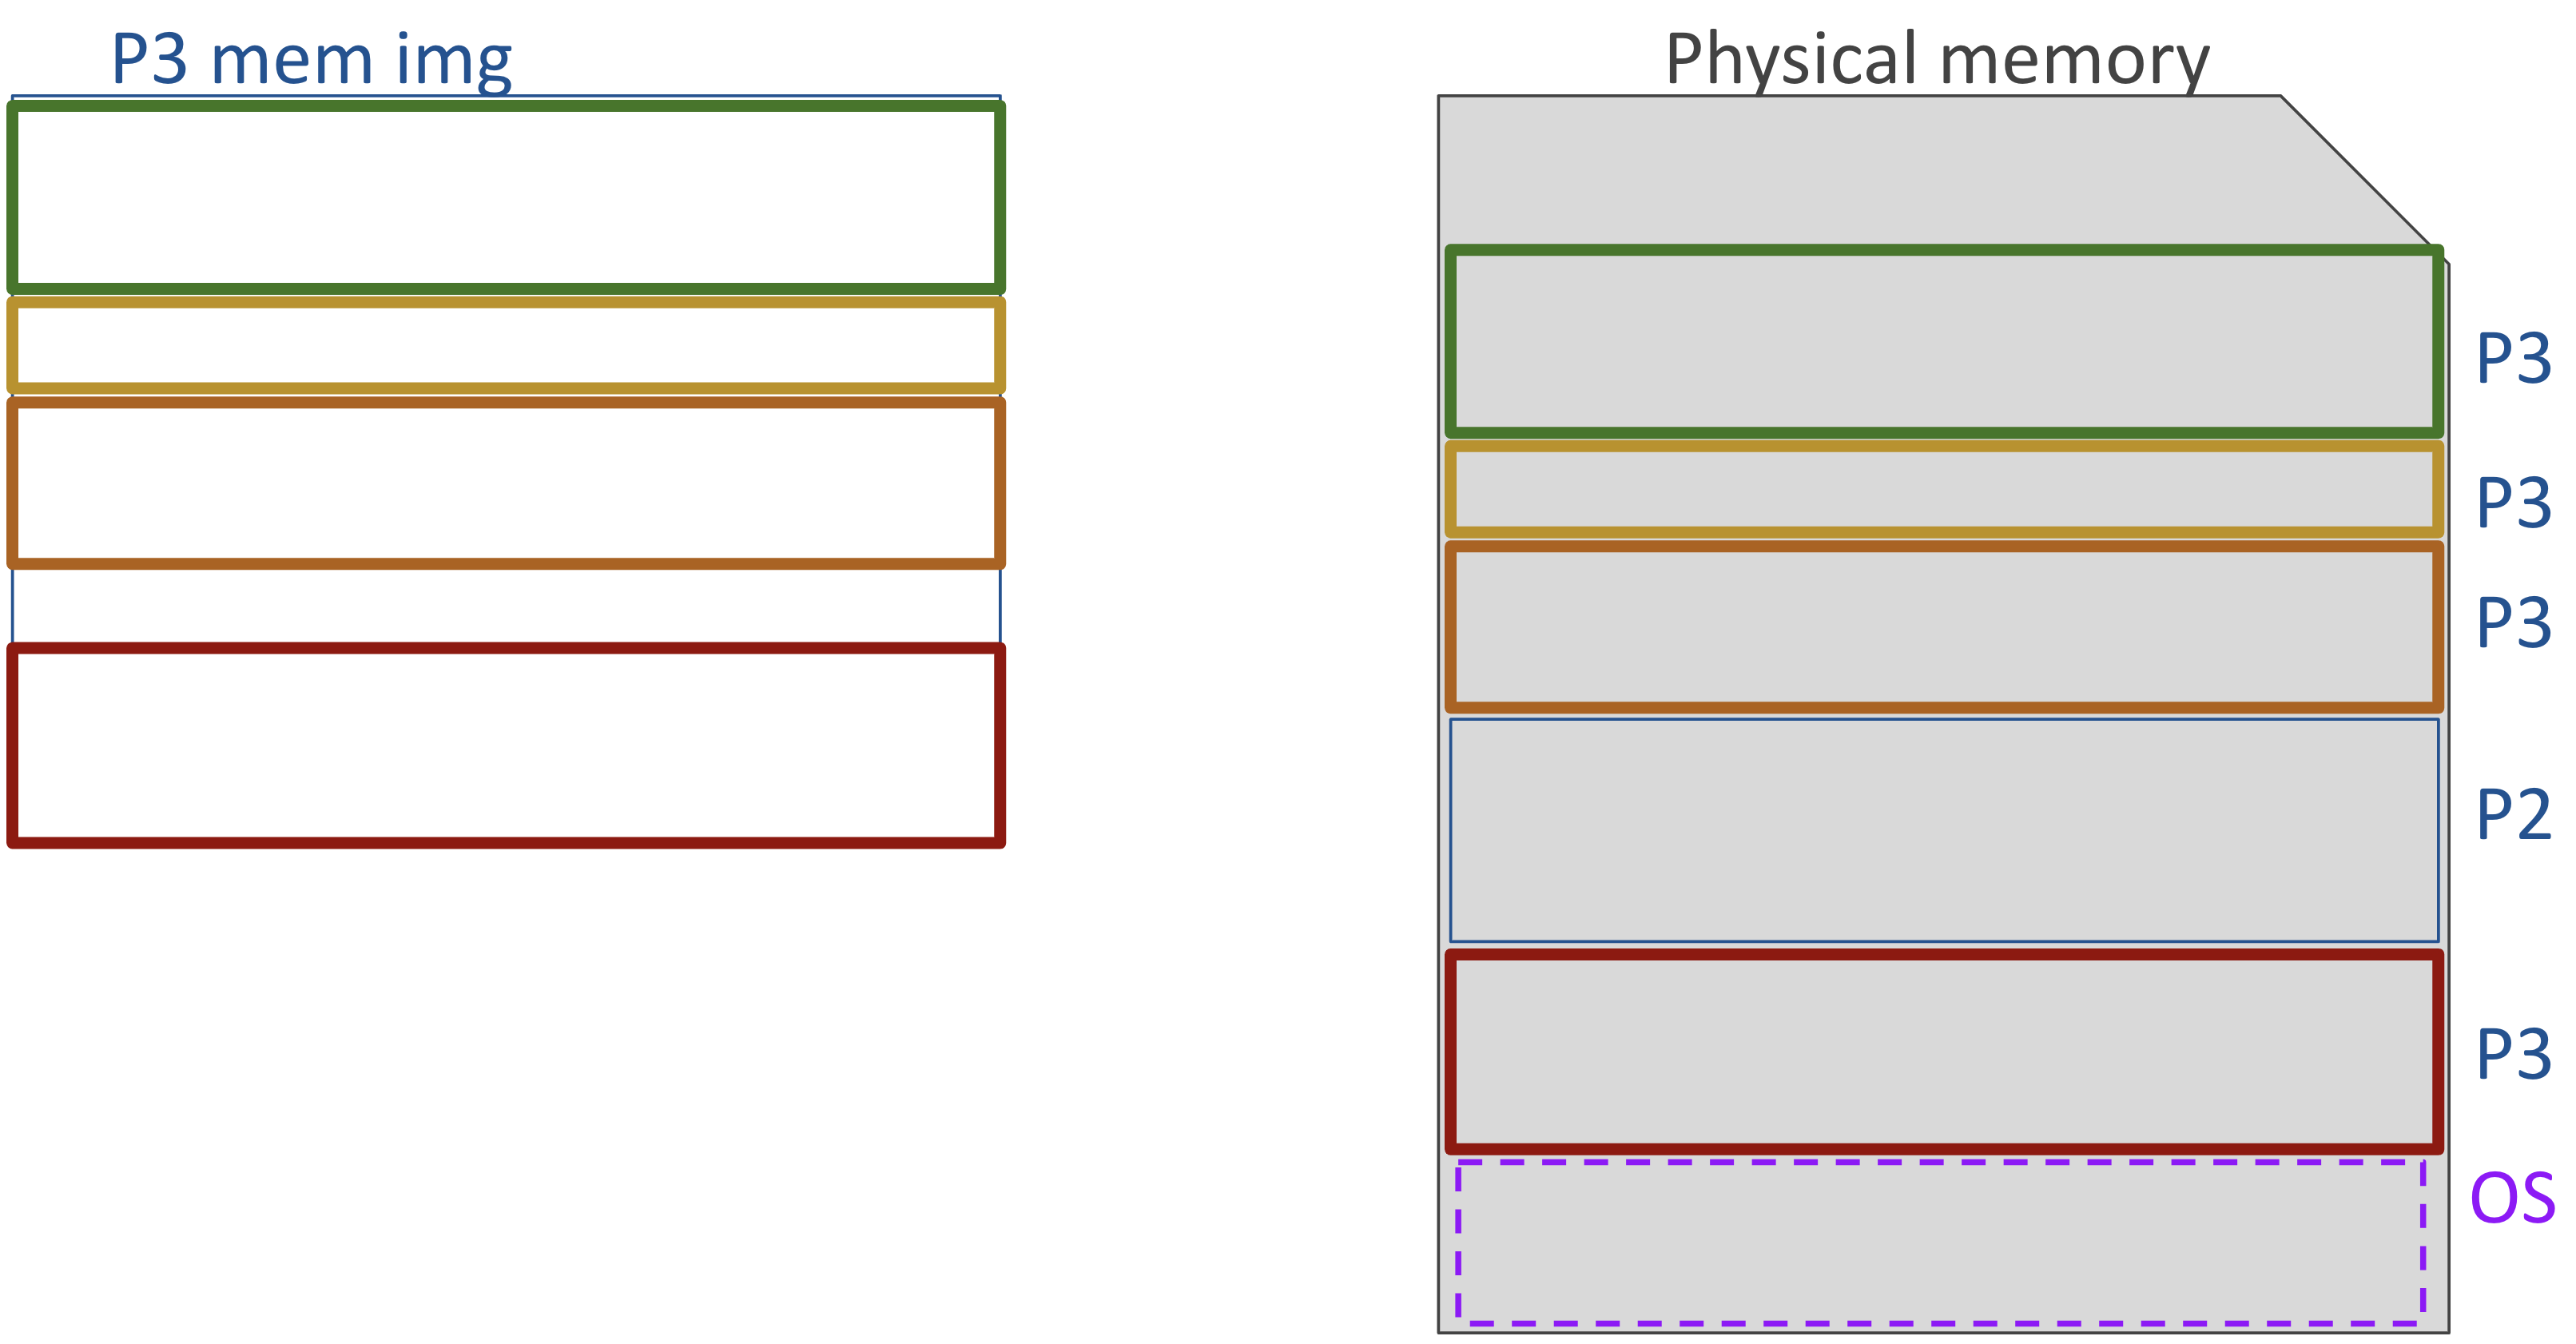
\includegraphics[width=1.25\textwidth]{chapters/L4/images/segmentation.png}
\end{center}
\end{minipage}
\\[20px]
\newpage
\noindent To address the inefficiency of requiring each process to occupy a single contiguous block of memory, an effective strategy is to \emph{divide the process’s address space into smaller chunks}, allowing noncontiguous allocation. Two primary techniques for accomplishing this are:
\vspace{10px}
\begin{itemize}
  \item[-] \textbf{Paging:} The address space is split into \emph{fixed-size pages}, which map onto equally sized \emph{physical frames}. This approach can reduce external fragmentation but can introduce \emph{internal fragmentation} if a process does not fully use the last frame of its allocation. Paging is straightforward to manage and scales well for large address spaces.
  \item[-] \textbf{Segmentation:} The address space is divided into \emph{variable-sized segments} (e.g., code, data, stack). This fits naturally with the logical structure of programs and can minimize \emph{internal} waste; however, it can result in \emph{external} fragmentation when segments cannot fit into available gaps in physical memory.
\end{itemize}

\begin{center}
  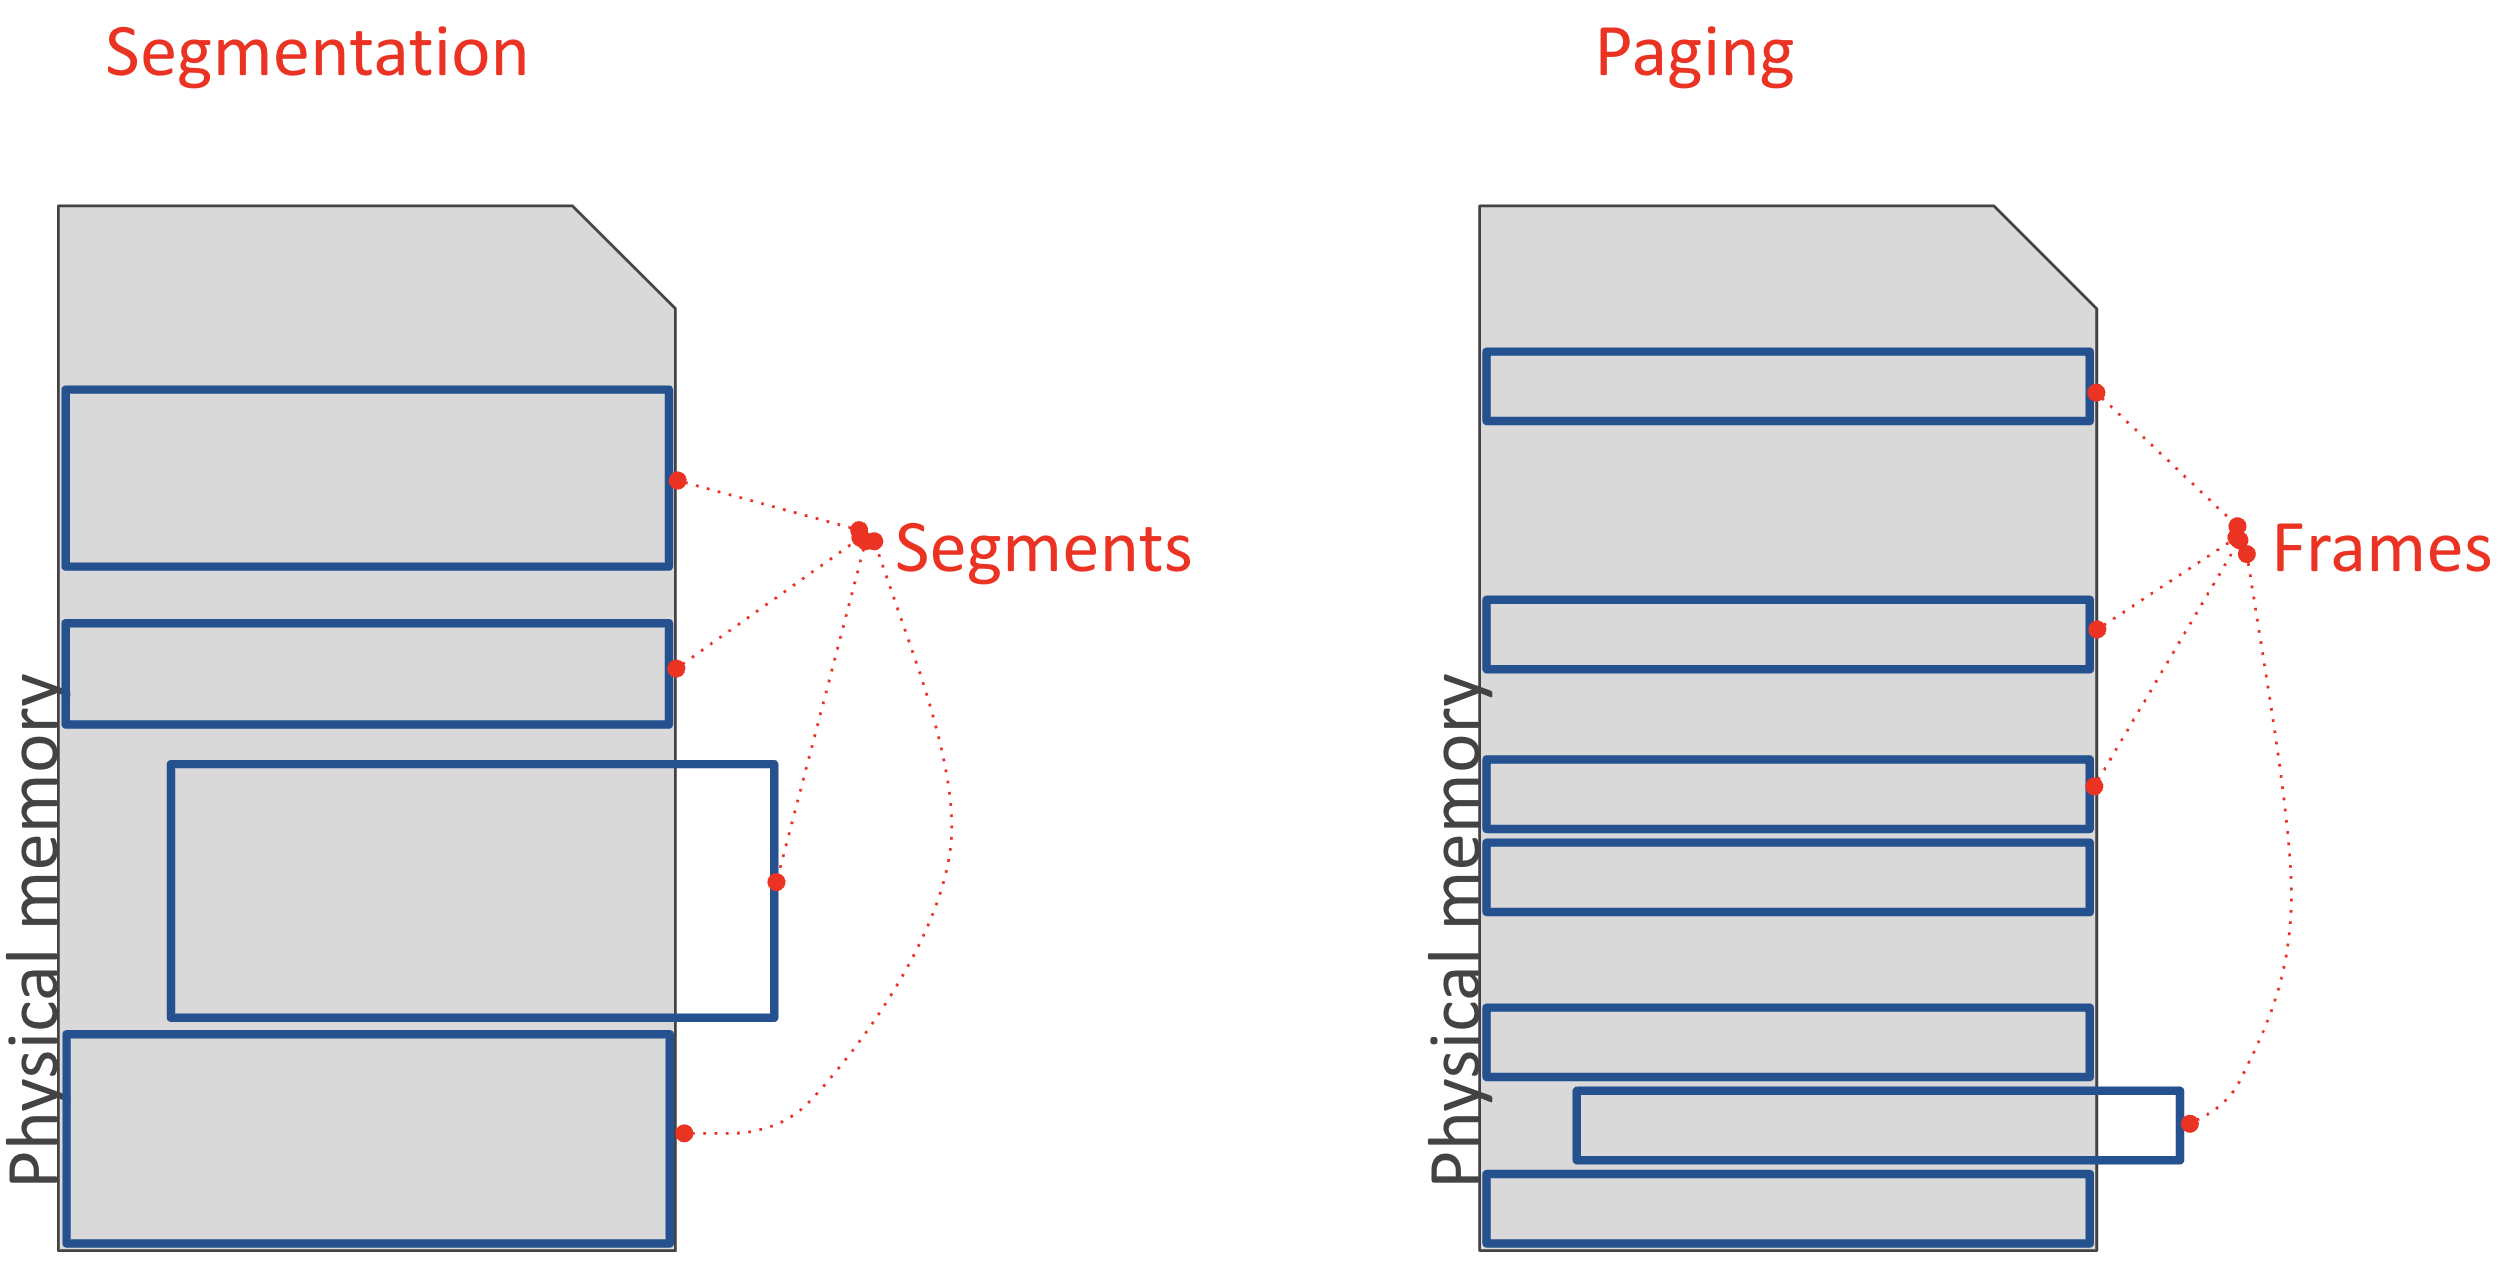
\includegraphics[width=0.65\textwidth]{chapters/L4/images/page-segment.png}
\end{center}

\noindent In \textbf{paging}, the MMU maintains a \emph{page table} to translate from virtual pages to fixed-size physical frames:

\begin{center}
  \includegraphics[width=0.65\textwidth]{chapters/L4/images/paging.png}
\end{center}

\noindent In either scheme, the MMU---\emph{configured} by the kernel with base, bound, or other address-translation structures---ensures each process can access only the memory it has been allocated. This \emph{hardware-based} translation mechanism preserves system safety and helps improve physical memory utilization by allowing noncontiguous allocation.
\newpage
\section{Optional - Operating System Mapping in Process Memory}
In modern operating systems, the OS is mapped into every process's virtual address space. This design allows a process to make system calls efficiently, as the CPU switches to pre-mapped high-address instructions during such transitions. This integration supports secure and fast interactions between user applications and system-level functions.

\begin{center}
  \includegraphics[width=0.55\textwidth]{chapters/L4/images/os-everywhere.png}
\end{center}

\section{CPU Caching and Memory Hierarchy}
Efficient computation in modern CPUs relies on a well-designed memory hierarchy that mitigates the performance gap between the processor and main memory. Central to this hierarchy is the CPU cache, which stores recently and frequently accessed data.

\subsection{Overview of CPU Cache}
The CPU cache is a small, high-speed memory located close to the processor core. It temporarily holds data and instructions that the CPU is likely to reuse, significantly reducing the latency compared to fetching data from main memory. This approach minimizes delays due to the slower speed of main memory and ensures smoother processor performance.
\begin{center}
  \includegraphics[width=0.55\textwidth]{chapters/L4/images/cpu-cache.png}
\end{center}

\subsection{Multi-Level Cache Architecture}
Modern CPUs employ a multi-level cache system to balance speed and storage capacity:

\begin{definition}[Cache Levels]
The cache hierarchy typically consists of:
\begin{itemize}
    \item \textbf{L\(_1\) Cache:} The smallest and fastest cache, often divided into separate instruction and data caches.
    \item \textbf{L\(_2\) Cache:} Larger than L\(_1\) and slightly slower, serving as an intermediary between L\(_1\) and L\(_3\).
    \item \textbf{L\(_3\) Cache:} The largest and slowest cache, usually shared among multiple cores in multi-core processors.
\end{itemize}
\end{definition}

The arrangement from smaller and faster (L\(_1\)) to larger and slower (L\(_3\)) reflects a deliberate trade-off between speed and capacity.

\begin{center}
  \includegraphics[width=0.55\textwidth]{chapters/L4/images/cpu-cache2.png}
\end{center}

\subsection{Cache Organization in Multi-Core Processors}
Today's processors often include multiple computing cores, each with dedicated L\(_1\) and L\(_2\) caches while sharing a common L\(_3\) cache. This design:
\begin{itemize}
    \item Provides high-speed access to data for individual cores.
    \item Balances the overall workload by reducing contention for shared resources.
\end{itemize}
Without such a hierarchical system, a single cache (e.g., L\(_1\)) might evict infrequently used yet critical instructions, thereby degrading performance.

\begin{example}
Consider a scenario in which a core with only an L\(_1\) cache continuously evicts a seldom-used, but vital instruction. The presence of additional cache levels (L\(_2\) and L\(_3\)) provides extra storage layers, ensuring that even infrequently accessed data remains available when needed.
\end{example}

\subsection{Summary of the Memory Hierarchy}
The overall memory hierarchy in a modern CPU is structured as follows:
\begin{enumerate}
    \item \textbf{L\(_1\) Cache:} Fastest, smallest, with separate instruction and data caches.
    \item \textbf{L\(_2\) Cache:} Intermediate in both size and speed.
    \item \textbf{L\(_3\) Cache:} Largest, slowest, shared among cores.
    \item \textbf{Main Memory:} Accessed only when data is not found in any cache.
\end{enumerate}
The CPU always accesses the memory hierarchy starting at the fastest level (L\(_1\)) and moving downward, ensuring that processing is carried out as efficiently as possible.
\end{document}

\documentclass[../../compsys.tex]{subfiles}
\begin{document}
\chapter{L5 - Paging}
\textit{Fellow syscoms, this is yet another chapter that was already studied in computer architecture, however, don't be discouraged, I'll do my best to make things clear. Again, please send me a text if anything lacks clarity, with that said, good luck.}\\[5px]
\textit{For context, we've established that a specialized hardware was required to efficiently translate virtual addresses into physical addresses. However, this introduces another critical requirement: optimizing memory usage. To address this, paging becomes essential, enabling dynamic memory allocation and effectively managing address space constraints.}
\vfill
\section{Page-based Memory Management Unit (MMU)}
In modern operating systems, paging is used to manage memory efficiently by dividing both the virtual address space and physical memory into fixed-size blocks. This section provides a detailed overview of how paging works and how addresses are translated.

\subsection{Overview of Paging}
\textit{Personal Remark:} Although the physical frames allocated to a process may be non-contiguous, the virtual address space appears contiguous to the process.\\
\noindent
\begin{minipage}{0.45\textwidth}
  \begin{itemize}
    \item[-] \textbf{Pages:} Fixed-size blocks that partition the virtual address space.
  \item[-] \textbf{Frames:} Fixed-size blocks that partition physical memory.
  \item[-] \textbf{Mapping:} Each page is associated with a frame via a mapping (i.e., \{page $\rightarrow$ frame\}). This allows the operating system to apply protection at the page level.
\end{itemize}
\end{minipage}
\hfill
\vline
\hfill
\begin{minipage}{0.45\textwidth}
\begin{center}
  \includegraphics[width=0.6\textwidth]{chapters/L5/images/page-mmu.png}
\end{center}
\end{minipage}\\
\newpage
\subsection{Size of a Page}
A page is the smallest unit of memory allocation in a paging system. Its size is chosen based on the following considerations:\\
\noindent
\begin{minipage}{0.45\textwidth}
\begin{itemize}
  \item[-] \textbf{Minimizing Internal Fragmentation:} Typical page sizes range from 4 KB to 16 KB.
  \item[-] \textbf{Management Overhead:} Smaller pages lead to larger page tables, while larger pages can waste memory.
\end{itemize}

\textbf{Super Pages:} These are larger blocks made up of multiple contiguous pages (e.g., 2 MB or 1 GB). They reduce the overhead associated with page translation. \\
\end{minipage}%
\hfill
\vline
\hfill
\begin{minipage}{0.45\textwidth}
\begin{center}
  \includegraphics[width=0.35\textwidth]{chapters/L5/images/page-size.png}
\end{center}
\end{minipage}\\

\subsection{Memory Management Scheme}
The operating system manages memory using the following scheme:\\[5px]
\noindent
\begin{minipage}{0.45\textwidth}
\begin{enumerate}
  \item \textbf{Frame Allocation:} Logical pages are mapped to available physical frames based on the OS's allocation strategy.
  \item \textbf{Page Table:} The OS maintains a data structure called the page table, which stores the mapping between logical pages and physical frames.
  \item \textbf{Per-Process Management:} Each process has its own page table to manage its virtual address space.
\end{enumerate}
\end{minipage}%
\hfill
\vline
\hfill
\begin{minipage}{0.45\textwidth}
  \begin{center}
    \includegraphics[width=0.45\textwidth]{chapters/L5/images/mapping.png}
  \end{center}
\end{minipage}

\subsection{Address Representation}
A virtual address is composed of two distinct components:
\begin{enumerate}
  \item \textbf{Virtual Page Number (VPN):} The higher-order \textit{p} bits of the address that identify the page in the virtual address space.
  \item \textbf{Page Offset:} The lower-order \textit{o} bits that specify the exact byte within the page.
\end{enumerate}

\begin{minipage}{\linewidth}
  \centering
  \includegraphics[width=0.65\textwidth]{chapters/L5/images/virtual.png}
\end{minipage}
\newpage
\begin{example}[Virtual Address Example (32-bit Architecture)]
In a 32-bit system, the virtual address is divided into a virtual page number and a page offset, as illustrated below.\\
\begin{center}
  \includegraphics[width=0.65\textwidth]{chapters/L5/images/paging-example.png}
\end{center}
\end{example}

\subsection{Address Translation}
Address translation is the process by which the Memory Management Unit (MMU) converts a virtual address into a physical address. The steps involved are:
\begin{enumerate}
  \item \textbf{Extract the Virtual Page Number:} Take the first \textit{p} bits of the virtual address.
  \item \textbf{Map to Physical Frame:} Use the page table to find the corresponding physical frame number.
  \item \textbf{Extract the Page Offset:} Take the remaining \textit{o} bits.
  \item \textbf{Compute the Physical Address:} Combine the frame number with the offset to access the specific byte in physical memory.
\end{enumerate}

\begin{center}
  \includegraphics[width=0.45\textwidth]{chapters/L5/images/translation.png}
\end{center}

\vspace{40px}
\subsubsection{Accessing a Byte}
To access a specific byte in memory, the MMU follows these steps:
\begin{enumerate}
  \item Extract the virtual page number from the virtual address.
  \item Map this virtual page number to the corresponding physical frame using the page table.
  \item Extract the offset from the virtual address.
  \item Access the byte at the calculated physical memory location.
\end{enumerate}

\textit{Personal Remark:} This systematic approach to address translation is fundamental to the operation of virtual memory systems, ensuring efficient and secure memory access.

\newpage
\subsection{Virtual Address Space}
\begin{example}[Virtual Address Space]
\leavevmode\\
\noindent
\begin{minipage}{0.55\textwidth}
  Consider a virtual address space consisting of 64 bytes, divided into 4 fixed-size pages of 16 bytes each. Assume all components of a program (code, stack, heap) comfortably fit into this address space.\\[5px]
\textbf{Question:} What is the size of a pointer necessary to uniquely address any byte in this address space?\\
\textbf{Answer:} 6 bits, since $\log_2(64) = 6$ bits are needed to uniquely represent each byte.
\end{minipage}%
\hfill
\vline
\hfill
\begin{minipage}{0.35\textwidth}
\begin{center}
  \includegraphics[width=0.45\textwidth]{chapters/L5/images/question.png}
\end{center}
\end{minipage}\\
\end{example}

\subsection{Physical Memory}

\begin{example}[Physical Memory]
\leavevmode
\\[2px]
Physical memory is composed of fixed-size storage slots called \textit{page frames}. Suppose there are 8 page frames, each 16 bytes, making the total physical memory 128 bytes. This setup requires at least 7 bits to uniquely represent any physical memory location ($\log_2(128) = 7$ bits). \\
\noindent
\begin{minipage}{0.45\textwidth}
The virtual pages of a process (e.g., process P1) map to physical memory frames as follows:\\

\begin{itemize}
  \item Virtual page 0 $\rightarrow$ Physical frame 3
  \item Virtual page 1 $\rightarrow$ Physical frame 7
  \item Virtual page 2 $\rightarrow$ Physical frame 5
  \item Virtual page 3 $\rightarrow$ Physical frame 2
\end{itemize}
\end{minipage}%
\hfill
\vline
\hfill
\begin{minipage}{0.45\textwidth}
\begin{center}
  \includegraphics[width=0.45\textwidth]{chapters/L5/images/paging-example2.png}
\end{center}
\end{minipage}
\\

\end{example}

\subsection{Virtual Address Translation}

\begin{example}[Virtual Address Translation]
\leavevmode \\[2px]
\noindent
\begin{minipage}{0.45\textwidth}
Consider that process P1 attempts to access a memory location using the following assembly instruction:
\[
\texttt{movl 21, \%eax}
\]
This instruction moves 4 bytes starting from virtual address 21 into the \%eax register. However, the data does not physically reside at virtual address 21; instead, it is stored in physical memory. Specifically, virtual address 21 belongs to virtual page 1, which maps to physical frame 7:
\end{minipage}%
\hfill
\vline
\hfill
\begin{minipage}{0.45\textwidth}
\begin{center}
  \includegraphics[width=0.9\textwidth]{chapters/L5/images/paging-example3.png}
\end{center}
\end{minipage}\\
\end{example}
\newpage
\begin{example}[Computing Virtual Page Number and Offset]
\leavevmode
\\[5px]
Given:
\begin{itemize}
  \item[-] Virtual address space: 64 bytes (6 bits)
  \item[-] Page size: 16 bytes (4 bits for offset)
\end{itemize}

Thus, the remaining $6 - 4 = 2$ bits represent the virtual page number.\\[5px]

\textbf{Question:} Determine the virtual page number and offset for the instruction \texttt{movl 21, \%eax}.

The binary representation of 21 is \texttt{010101}. Thus:
\begin{itemize}
  \item Virtual page number: first 2 bits (01) $\rightarrow$ Page 1
  \item Offset: last 4 bits (0101)
\end{itemize}

Given the page table mapping, virtual page 1 corresponds to physical frame 7 (binary \texttt{111}):

\begin{center}
  \includegraphics[width=0.85\textwidth]{chapters/L5/images/paging-example4.png}
\end{center}
\end{example}

\section{The Page Table}

\begin{definition}[Page Table]
\leavevmode
\\[2px]
A \textbf{page table} is a data structure maintained by the operating system that stores the mapping between virtual addresses and their corresponding physical addresses. Each process has its own dedicated page table.

The pointer to the currently active page table is stored in a special register known as the \textit{page-table base register} (PTBR). On x86 architectures, this register is typically referred to as \texttt{\%cr3}. During context switches, the operating system saves and restores the PTBR value from the process control block (PCB).
\end{definition}
\subsection{Structure of Page Table Entries}
The page table consists of multiple \textbf{page table entries} (PTEs). Each entry stores not only the \textit{page frame number} (PFN) that provides the mapping between virtual pages and physical frames but also additional status information. Important fields in a PTE typically include:

\begin{itemize}
  \item[-] \textbf{Present bit}: Indicates if the translation is valid and the page resides in physical memory.
  \item[-] \textbf{Protection bits}: Define access permissions (read, write, execute).
  \item[-] \textbf{User/Supervisor bit (U/S)}: Differentiates between user-mode and kernel-mode access permissions.
  \item[-] \textbf{Dirty bit}: Indicates if the page has been modified (written to).
  \item[-] \textbf{Access/Reference bit}: Used to track page usage patterns and inform page replacement algorithms.
\end{itemize}
\newpage
Below, the 32-bit Intel PTE format
\begin{center}
  \includegraphics[width=0.85\textwidth]{chapters/L5/images/intel.png}
\end{center}

Additionally, each page table entry is always aligned to the page size for efficient access by the hardware.


\section{Organizing the Page Table Structure}

The simplest implementation is the \textbf{linear page table}. The Memory Management Unit (MMU) indexes directly into the page table using the \emph{virtual page number}.

The process involves the following steps:
\begin{enumerate}
    \item The MMU uses the virtual page number as an index into the linear array of page table entries.
    \item It retrieves the corresponding \emph{page table entry (PTE)} at this index.
    \item From the PTE, the MMU obtains the associated \emph{physical frame number}.
\end{enumerate}

A linear page table requires the allocation of multiple contiguous memory pages to store the entire mapping structure.

\begin{center}
  \includegraphics[width=0.55\textwidth]{chapters/L5/images/pte.png}
\end{center}

\begin{example}[Size of a Linear Page Table]
Consider the following assumptions:
\begin{itemize}
  \item[-] Virtual address size: 32 bits
  \item[-] Physical address size: 32 bits
  \item[-] Page size: 4 KB (i.e., 12 bits offset)
  \item[-] Each page table entry (PTE): 4 bytes
\end{itemize}

The size of the linear page table is calculated as follows:

\[
\text{Number of entries} = 2^{\text{Virtual Address Bits} - \text{Offset Bits}} = 2^{32 - 12} = 2^{20}
\]

Thus, the page table size is:

\[
\text{Page Table Size} = \text{Number of Entries} \times \text{Size per Entry} = 2^{20} \times 4\text{ bytes} = 4\text{ MiB}
\]
\end{example}
\vfill
\newpage
\subsection{Resolving addresses with a Linear Page Table (32-bit)}
In a 32-bit linear paging system, the address translation process from virtual to physical addresses follows a straightforward mechanism, detailed step-by-step below and illustrated bellow. 

\begin{enumerate}
    \item \textbf{Access Address Breakdown}
    \begin{itemize}
      \item[] The virtual (logical) address consists of two parts
        \begin{enumerate}
            \item \textbf{Page number} identifies the page in virtual memory.
            \item \textbf{Offset} identifies the byte within the page.
        \end{enumerate}
        For example, the address \texttt{20 983 809} can be split into:
        \begin{itemize}
            \item Page number \texttt{5123}
            \item Offset \texttt{1}
        \end{itemize}
    \end{itemize}

    \item \textbf{Lookup in Page Table}
    \begin{itemize}
        \item The Page Table Base Register (PTBR) points to the beginning of the page table in physical memory (in our example, \texttt{PTBR = 0x0}).
        \item The page number extracted from the virtual address (\texttt{5123}) is used as an index into the linear page table.
    \end{itemize}

    \item \textbf{Page Frame Identification} The entry at index \texttt{5123} in the page table provides the frame number in physical memory (in the diagram example, frame number \texttt{1026}).


    \item \textbf{Physical Address Computation}
    \begin{itemize}
        \item The physical frame number (\texttt{1026}) obtained from the page table and the original offset (\texttt{1}) from the virtual address are combined to form the physical address.
        \item This address directly maps to a unique location in physical memory.
    \end{itemize}

    \item \textbf{Accessing the Memory} Finally, the computed physical address is used to access the desired data in physical memory.
\end{enumerate}

\begin{center}
  \includegraphics[width=0.65\textwidth]{chapters/L5/images/resolving.png}
\end{center}

This linear mapping approach is simple and direct but may require substantial memory for the page table, especially when handling large virtual address spaces, let's see how much.

\subsection{The Issue with Linear Page Tables (4 KB Pages)}

Using a linear page table with a 32-bit architecture, a 4 KB (12-bit offset) page size, and 4-byte entries results in a considerable memory overhead:
\[
\text{Number of entries} = 2^{32 - 12} = 2^{20}
\]
\[
\text{Page table size} = 2^{20} \times 4\,\text{bytes} = 4\,\text{MiB}
\]

Expanding this to 64-bit architectures significantly increases memory usage:

\begin{center}
\small
\begin{tabular}{|c|c|c|c|}
\hline
\textbf{Virtual Address Bits} & \textbf{Physical Address Bits} & \textbf{Entry Size} & \textbf{Page Table Size} \\
\hline
32 & 48 bit & 8 bytes & 8 MiB \\
64 & 64 bit & 8 bytes & $2^{52} \times 8$ bytes = 32 PiB \\
\hline
\end{tabular}
\end{center}
\normalsize
In 64-bit architectures with large, sparse address spaces, linear page tables quickly become impractical. Although increasing the page size (e.g., from \(16\,\mathrm{KiB}\) pages) can reduce memory overhead, it introduces significant internal fragmentation. Let's look at a more effective approach
\subsection{Multi-level Page Tables}
\small
Most processes use only a small fraction of the available address space. Multi-level page tables efficiently allocate metadata only for the used portion by organizing the page table in a hierarchy. Although each level adds an extra memory lookup during address translation, this method saves space overall. \\[5px]
\textbf{Analogy} Imagine locating a book in a library: first, you choose a section, then an aisle, then a shelf, and finally the book's position. \\[5px]
\textbf{Analogy 2  - This made me understand how multi-level paging is more memory efficient}\\
Imagine organizing a large library. \\[4px]
With a \textbf{linear (single-level) page table}, you'd have to create a catalog entry for \textit{every shelf}—even if most shelves are completely empty. This wastes space by reserving entries for unused shelves. \\[4px]
A \textbf{two-level page table} solves this problem by using a hierarchical catalog: the \textit{first-level catalog} only keeps track of sections of shelves that actually contain books. Detailed \textit{second-level catalogs} are created solely for these used sections, avoiding unnecessary records for empty shelves and significantly reducing memory usage.\\

\begin{example}[Two-Level Paging Example]
A virtual address on a 32-bit machine with a 4~KiB page size is divided as follows:
\begin{itemize}
  \item \textbf{Page offset:} 12 bits.
  \item \textbf{Page number:} 20 bits.
\end{itemize}
Since the page table is paged, the 20-bit page number is split into two 10-bit parts:
\begin{itemize}
  \item The first 10 bits index the first-level page table.
  \item The next 10 bits index the second-level page table.
\end{itemize}
With each page table entry occupying 4 bytes, a 4~KiB page can hold up to $\frac{4096}{4} = 1024 \quad (\text{or } 1 \ll 10) \quad \text{entries}$. \\
\noindent
\begin{minipage}{0.40\textwidth}
\begin{center}
  \includegraphics[width=0.9\textwidth]{chapters/L5/images/two-level-address.png}
\end{center}
\end{minipage}%
\hfill
\vline
\hfill
\begin{minipage}{0.50\textwidth}
\begin{center}
  \includegraphics[width=1.1\textwidth]{chapters/L5/images/two-level-diagram.png}
\end{center}
\end{minipage}
\end{example}
\normalsize
\subsection{Resolving Addresses: Linear vs.\ Two-Level Paging (32-bit)}
\noindent
\begin{minipage}{0.42\textwidth}
\footnotesize
In a \emph{linear} (single-level) paging scheme for a 32-bit address space, the virtual address is typically split into two parts: 
\[
\underbrace{\text{Page Number}}_{20 \text{ bits}} \quad \underbrace{\text{Offset}}_{12 \text{ bits}}.
\]
The \emph{page number} serves as an index into a single page table, which holds the base address of the corresponding physical page. The \emph{offset} is then added to this base address to obtain the final physical address.

By contrast, in a \emph{two-level paging} scheme, the 20-bit page number is further subdivided into:
\[
\underbrace{\text{Page Directory Index}}_{10 \text{ bits}} 
\quad
\underbrace{\text{Page Table Index}}_{10 \text{ bits}}
\quad
\underbrace{\text{Offset}}_{12 \text{ bits}}.
\]
The top 10 bits (page directory index) point to an entry in the \emph{page directory}, which in turn identifies the base address of a particular \emph{page table}. The next 10 bits (page table index) select the entry in that page table, which gives the base address of the physical page. Finally, the offset is added to this base address to compute the physical address.\\[5px]
The main difference is that \emph{linear paging} uses a single, large page table for the entire virtual address space, whereas \emph{two-level paging} uses a hierarchy of smaller tables. 
\end{minipage}%
\hfill
\vline
\hfill
\begin{minipage}{0.55\textwidth}
  \begin{center}
    \includegraphics[width=1.2\textwidth]{chapters/L5/images/vs.png}
  \end{center}
\end{minipage}\\

\subsection{Multi-level Page Table for 64-bit Addressing}
In systems with a 4\,KiB page size (4096 bytes), each page holds 512 page table entries because 
\[
4096 \text{ bytes} \div 8 \text{ bytes/entry} = 512 \text{ entries} \quad (\text{requiring } 9 \text{ bits since } 2^9 = 512).
\]
For a full 64-bit address, subtracting the 12 bits used for the page offset leaves 52 bits to be mapped. A common scheme uses five levels of page tables for the first 45 bits (5 levels $\times$ 9 bits each) and a sixth level for the remaining 7 bits. If the virtual address space is reduced:
\begin{itemize}
  \item[-] To 57 bits: $57 - 12 = 45$ bits remain, which can be mapped with 5 levels.
  \item[-] To 48 bits: $48 - 12 = 36$ bits remain, requiring 4 levels.
\end{itemize}

\subsection{Paging: Advantages and Disadvantages}
\textbf{Advantages:}
\begin{itemize}
    \item \emph{No external fragmentation:} Memory is allocated in fixed-size pages.
    \item \emph{Fast allocation and deallocation:} Pages can be allocated or freed without searching for a contiguous memory block.
\end{itemize}

\textbf{Disadvantages:}
\begin{itemize}
    \item \emph{Memory overhead:} Additional space is required to store the page tables.
    \item \emph{Increased memory accesses:} Each memory access may require extra references to the page tables.
    \item \emph{Hardware complexity:} Efficient address translation demands specialized hardware (eg. we'll look at that hardware in the next section)
  \end{itemize}

\subsection{Logical Process of Memory Access in a Paging System}
When the CPU requests a code or data value at a virtual address, the following steps occur:
\begin{enumerate}
    \item The Memory Management Unit (MMU) begins a page table walk starting from the Page Table Base Register (PTBR).
    \item Depending on the address space:
    \begin{itemize}
      \item[-] A 32-bit address may require 2 memory references for translation.
      \item[-] A 48-bit address may require up to 4 memory references.
    \end{itemize}
    \item After the page table lookup, the page offset is added to the translated address to access the actual data in physical memory.
    \item To reduce the translation overhead, a cache called the Translation Lookaside Buffer (TLB) is used to store recent virtual-to-physical address mappings.
\end{enumerate}


\section{Translation Lookaside Buffer (TLB)}
\textit{Seen in a comparch, I'll try to make this clear.}\\

The Translation Lookaside Buffer (TLB) is a specialized, hardware-based cache that stores recent mappings from virtual addresses to physical addresses. When a process accesses memory, the Memory Management Unit (MMU) first checks the TLB:
\begin{itemize}
  \item[-] \textbf{TLB Hit:} If the mapping is present, the physical address is obtained directly, minimizing delay.
  \item[-] \textbf{TLB Miss:} If the mapping is absent, the MMU must perform a page table walk, involving multiple memory accesses, which is significantly slower.
\end{itemize}

The effectiveness of the TLB is largely due to the principle of locality of reference, which ensures a high hit rate under typical workloads. However, TLB entries can become invalid after a context switch or when page tables are updated.

\subsection{Memory Access Cost}
Assume a 64-bit address space and that all page table levels are cached when the TLB is present (i.e., on a TLB hit). The following table illustrates the number of memory accesses required to read or write a memory location \(X\) for a process:

\begin{center}
\begin{tabular}{l|c|c}
    \toprule
    \textbf{Page Table Level} & \textbf{With TLB \& TLB Hit} & \textbf{Without TLB} \\
    \midrule
    No Paging & 1 & 1 \\
    1 Level   & 1 & 2 \\
    2 Level   & 1 & 3 \\
    3 Level   & 1 & 4 \\
    \bottomrule
\end{tabular}
\end{center}

\textbf{Key:} The TLB is implemented as a dedicated circuit, separate from main memory, enabling rapid address translation.
\newpage
\subsection{TLB Lookup Process}
A Translation Lookaside Buffer (TLB) is a small, fast cache that stores recent virtual-to-physical address translations to speed up memory accesses. \\[9px]
\noindent
\begin{minipage}{0.45\textwidth}
\small
\begin{enumerate}
    \item \textbf{Decompose the virtual address:} 
    The processor splits the virtual address into two parts:
    \begin{itemize}
        \item \textit{Virtual Page Number (VPN)}: The high-order bits used for indexing or tagging in the TLB.
        \item \textit{Offset}: The low-order bits that remain unchanged when forming the physical address.
    \end{itemize}
    
    \item \textbf{Check the TLB:} The VPN is compared against the \emph{tag} fields of all TLB entries (often in parallel, if the TLB is fully associative). If a matching tag is found, it indicates a potential translation match.

    \item \textbf{Validate the match:}
    Along with the tag comparison, each TLB entry includes \emph{valid} and possibly other \emph{protection} bits. The processor checks these bits to ensure:
    \begin{itemize}
        \item The entry is valid (i.e., not stale or invalidated).
        \item The access permissions allow the requested operation (read, write, or execute).
    \end{itemize}
    If these checks pass, the match is confirmed.

    \item \textbf{Obtain the physical frame number (PFN):} Upon a valid match, the TLB entry provides the corresponding \emph{Physical Frame Number} (PFN). This is combined with the original offset to form the final physical address.

    \item \textbf{Handle TLB misses:}
    If no valid TLB entry matches the VPN (Virtual Page Number):
    \begin{itemize}
        \item The hardware (or the operating system, depending on the architecture) performs a \emph{page table walk} to locate the correct PFN in the page table.
        \item The discovered translation may then be loaded into the TLB for future accesses.
        \item The instruction or memory operation is retried with the updated TLB entry.
    \end{itemize}
\end{enumerate}
\end{minipage}%
\hfill
\vline
\hfill
\begin{minipage}{0.45\textwidth}
  \begin{center}
    \includegraphics[width=1.25\textwidth]{chapters/L5/images/tlb.png}
  \end{center}
\end{minipage}\\[9px]

This process allows the CPU to translate virtual addresses into physical addresses quickly by leveraging the TLB's cached entries, significantly reducing the average memory access time.
\newpage
\subsection{CPU Execution of a Read/Write Operation}
\begin{enumerate}
    \item The CPU issues a load operation for a given virtual address (as part of a memory load/store).
    \item The Memory Management Unit (MMU) checks the Translation Lookaside Buffer (TLB) for the virtual address.
    \item \textbf{TLB Miss:}
    \begin{itemize}
        \item The MMU performs a page walk through the page table.
        \item If the Page Table Entry (PTE) is not present, a page fault occurs; the OS is invoked and a segmentation fault may be raised.
        \item If the PTE is present, the TLB is updated and execution continues.
    \end{itemize}
    \item \textbf{TLB Hit:} The physical address is obtained from the TLB, the memory location is fetched, and the data is returned to the CPU.
\end{enumerate}

\subsection{Summary: Page Tables}
\begin{itemize}
  \item[-] \textbf{Contents:} Page Table Entries (PTEs) that include permission bits.
  \item[-] \textbf{Size:} 
    \begin{itemize}
      \item[-] \textit{Linear Page Table:} Can be very large.
      \item[-] \textit{Multi-Level Page Table:} More memory efficient when sparsely populated.
    \end{itemize}
  \item[-] \textbf{Performance:} Paging overhead is mitigated by the use of the TLB.
  \item[-] \textbf{Memory Exhaustion:} Appropriate measures must be taken when the system runs out of memory.
\end{itemize}
\section{Swapping: Managing Memory Shortages}
When the physical memory is insufficient to hold all the active processes, the operating system (OS) employs a mechanism called \emph{swapping}. This process involves temporarily moving pages that are not actively used from main memory to disk storage. By doing so, the OS can reclaim memory for processes that require immediate attention and even over-provision memory beyond the available physical resources.

\subsection{Concepts}
\begin{itemize}
  \item[-] \textbf{Working Set:} The collection of pages a process actively uses at a given time. This set can change dynamically as the process executes.
  \item[-] \textbf{Storing Unused Pages:} By transferring inactive pages to disk, the OS frees up main memory for active processes.
  \item[-] \textbf{Over-Provisioning:} Swapping allows the system to allocate more virtual memory than is physically available.
\end{itemize}
\newpage
\subsection{Swapping In: Handling Page Faults}
When a process accesses a page that is not present in main memory, the Memory Management Unit (MMU) cannot translate the virtual address because the corresponding page table entry indicates that the page is absent. This situation results in a \emph{page fault}, prompting the OS to bring the page back from disk (swap-in).

\subsubsection{Page Fault Handling Procedure}
\begin{enumerate}
    \item \textbf{Address Translation:} The MMU translates virtual addresses to physical addresses using page tables. Each page table entry has a \textit{present bit} indicating if the page is in memory.
    \item \textbf{Page Fault Occurrence:} If the present bit is unset, a page fault is triggered.
    \item \textbf{Identifying the Fault:} The OS determines which process and address caused the fault by consulting its data structures.
    \item \textbf{Determining Page Status:}
    \begin{itemize}
        \item If the page is on disk, the OS issues a request to load it into memory.
        \item If the page has not been swapped out, the OS creates the mapping and updates its data structures.
    \end{itemize}
    \item \textbf{Context Switching:} While waiting for disk I/O, the OS may switch to another process.
    \item \textbf{Resuming Execution:} Once the page is loaded, the OS updates the page table entry and the Translation Lookaside Buffer (TLB), and then resumes the faulting process.
\end{enumerate}

\subsubsection{Swap-In Procedure}
\noindent
\begin{minipage}{0.45\textwidth}
\begin{enumerate}
    \item Locate the page in the swap cache.
    \item Allocate a new page in memory.
    \item Copy the content from disk to the allocated page.
    \item Update the page table entry to indicate that the page is now in memory.
    \item Load the corresponding TLB entry.
\end{enumerate}
\end{minipage}%
\hfill
\begin{minipage}{0.45\textwidth}
\begin{center}
\includegraphics[width=1.1\textwidth]{chapters/L5/images/swapin.png}
\end{center}
\end{minipage}
\newpage
\subsection{Swapping Out: Freeing Up Memory}
Swapping out is the process of moving pages from main memory to disk, thereby freeing up physical memory for active processes. Although the steps involved are straightforward, choosing which pages to swap out is governed by complex OS policies to avoid performance degradation (e.g., thrashing).

\subsubsection{Swap-Out Procedure}
\noindent
\begin{minipage}{0.45\textwidth}
\begin{enumerate}
    \item Invalidate the corresponding TLB entry.
    \item Allocate an entry in the designated swap space.
    \item Copy the page content from memory to disk.
    \item Update the page table entry to reflect that the page is now stored on disk.
    \item Release the physical memory page.
\end{enumerate}
\end{minipage}%
\hfill
\begin{minipage}{0.45\textwidth}
\begin{center}
  \includegraphics[width=1.1\textwidth]{chapters/L5/images/swapout.png}
\end{center}
\end{minipage}

\subsection{Conclusion}
Swapping is a vital mechanism in memory management, enabling the OS to manage limited physical memory efficiently by transferring inactive pages to disk. This dynamic exchange between main memory and disk ensures that active processes have the resources they need while also allowing the system to support a larger number of processes. However, careful policy decisions are essential to minimize overhead and avoid issues such as thrashing.
\end{document}


\end{document}
